% paper2/tex/main.tex -- paper 2 manuscript. Built through anonymous.tex (TMLR double-blind) or preprint.tex (arXiv).
% Do not compile main.tex directly: the wrapper defines \PREPRINT (or not) and % paper2/tex/main.tex -- paper 2 manuscript. Built through anonymous.tex (TMLR double-blind) or preprint.tex (arXiv).
% Do not compile main.tex directly: the wrapper defines \PREPRINT (or not) and % paper2/tex/main.tex -- paper 2 manuscript. Built through anonymous.tex (TMLR double-blind) or preprint.tex (arXiv).
% Do not compile main.tex directly: the wrapper defines \PREPRINT (or not) and % paper2/tex/main.tex -- paper 2 manuscript. Built through anonymous.tex (TMLR double-blind) or preprint.tex (arXiv).
% Do not compile main.tex directly: the wrapper defines \PREPRINT (or not) and \input{main}.
% Generated parts (do not edit by hand; run build_tex.py): title.tex, body.tex, appendixA-E.tex.
\documentclass[10pt]{article}
\ifdefined\PREPRINT
  \usepackage[preprint]{tmlr}
\else
  \usepackage{tmlr}
\fi
\usepackage[utf8]{inputenc}
\usepackage{amsmath,amssymb}
\usepackage{graphicx}
\usepackage{booktabs}
\usepackage{longtable}
\usepackage{array}
\usepackage{url}
\usepackage[hidelinks]{hyperref}
\graphicspath{{../figures/}}
\newcolumntype{R}[1]{>{\raggedright\arraybackslash}p{#1}}

\input{title.tex}

\ifdefined\PREPRINT
  \author{\name Gelavizh Ahmadi \\
          \addr Independent researcher, Berlin, Germany \\
          \addr ORCID: 0000-0000-0000-0000 % ORCID-PLACEHOLDER: replace before posting
          }
  \newcommand{\figname}[1]{(\texttt{#1})}
  \newcommand{\REPOSTATEMENT}{Code, committed results and figure scripts: \url{https://github.com/drgelavizhahmadi-dotcom/battery_hacketon}.}
  \hypersetup{pdftitle={Runaway edges: a smoothness-penalty blind spot makes Kolmogorov-Arnold networks non-identifiable on correlated inputs},
              pdfauthor={Gelavizh Ahmadi}}
\else
  % anonymous build: no author, affiliation, acknowledgments or repository URL anywhere in the source that reaches the PDF
  \author{}
  \newcommand{\figname}[1]{}
  \newcommand{\REPOSTATEMENT}{Code will be released upon publication.}
  \hypersetup{pdftitle={Runaway edges: a smoothness-penalty blind spot makes Kolmogorov-Arnold networks non-identifiable on correlated inputs},
              pdfauthor={}, pdfsubject={}, pdfkeywords={}, pdfcreator={LaTeX}}
\fi

\begin{document}
\maketitle

\input{body.tex}

\bibliography{references}
\bibliographystyle{tmlr}

\appendix
\ifdefined\PREPRINT
  \input{appendixA.tex}\input{appendixB.tex}\input{appendixC.tex}\input{appendixD.tex}\input{appendixE.tex}
\else % commit hashes replaced by neutral labels (commitmap.json is not part of the submission)
  \input{appendixA_anon.tex}\input{appendixB_anon.tex}\input{appendixC_anon.tex}\input{appendixD_anon.tex}\input{appendixE_anon.tex}
\fi

\end{document}
.
% Generated parts (do not edit by hand; run build_tex.py): title.tex, body.tex, appendixA-E.tex.
\documentclass[10pt]{article}
\ifdefined\PREPRINT
  \usepackage[preprint]{tmlr}
\else
  \usepackage{tmlr}
\fi
\usepackage[utf8]{inputenc}
\usepackage{amsmath,amssymb}
\usepackage{graphicx}
\usepackage{booktabs}
\usepackage{longtable}
\usepackage{array}
\usepackage{url}
\usepackage[hidelinks]{hyperref}
\graphicspath{{../figures/}}
\newcolumntype{R}[1]{>{\raggedright\arraybackslash}p{#1}}

\title{Runaway edges: a smoothness-penalty blind spot makes Kolmogorov--Arnold networks non-identifiable on correlated inputs}


\ifdefined\PREPRINT
  \author{\name Gelavizh Ahmadi \\
          \addr Independent researcher, Berlin, Germany \\
          \addr ORCID: 0000-0000-0000-0000 % ORCID-PLACEHOLDER: replace before posting
          }
  \newcommand{\figname}[1]{(\texttt{#1})}
  \newcommand{\REPOSTATEMENT}{Code, committed results and figure scripts: \url{https://github.com/drgelavizhahmadi-dotcom/battery_hacketon}.}
  \hypersetup{pdftitle={Runaway edges: a smoothness-penalty blind spot makes Kolmogorov-Arnold networks non-identifiable on correlated inputs},
              pdfauthor={Gelavizh Ahmadi}}
\else
  % anonymous build: no author, affiliation, acknowledgments or repository URL anywhere in the source that reaches the PDF
  \author{}
  \newcommand{\figname}[1]{}
  \newcommand{\REPOSTATEMENT}{Code will be released upon publication.}
  \hypersetup{pdftitle={Runaway edges: a smoothness-penalty blind spot makes Kolmogorov-Arnold networks non-identifiable on correlated inputs},
              pdfauthor={}, pdfsubject={}, pdfkeywords={}, pdfcreator={LaTeX}}
\fi

\begin{document}
\maketitle

% GENERATED by build_tex.py from paper2/draft/paper2_draft.md -- do not edit by hand
\begin{abstract}
Kolmogorov--Arnold networks (KANs) are promoted as interpretable because each edge carries a learned univariate function. We show that a widely used family of smoothness penalties leaves a blind spot that undermines this promise: second-difference and curvature penalties do not charge for affine components of an edge, and SiLU base weights are often unpenalised. When the inputs to a layer are correlated, affine components on different edges can cancel inside a unit, so training inflates the parameters along directions that neither the penalty nor the data can see; the loss has no reachable finite minimum and independent runs never agree. In a pre-registered synthetic study with a known teacher, correlated inputs gave 0 of 16 converged models (median squared-norm growth 32--66$\times$), including under a recently proposed curvature penalty that also penalises the SiLU weight, while a small penalty on the affine null space gave 16 of 16 certified minima and exact recovery of the teacher's internals. On real electrolyte-conductivity data the same mechanism explains why no model converged, and polishing beyond early stopping under a weak null-space penalty degraded held-out accuracy (RMSE 0.142 $\to$\allowbreak{} 1.03). Closing the blind spot restores certified minima but leaves several distinct minima, so convergence and identifiability are separate problems. We give practical recommendations for penalised KANs.

\end{abstract}

\section{Introduction}\label{sec:1}

KANs replace a network's fixed activations with learned univariate functions on every edge. Their appeal for science rests on reading those functions: an edge that looks like an exponential decay suggests a physical law. That reading presumes the edges are determined by the data. If different training runs produce different edges with equally good predictions, the edges describe the optimiser, not the system.

This paper identifies a concrete, common mechanism that breaks that presumption. It arises from the interaction of three ingredients that are each standard in practice:

\begin{enumerate}
  \item \textbf{A smoothness penalty with an affine null space.} Second-difference (P-spline) penalties and curvature penalties ignore straight-line components of an edge; SiLU base terms are frequently unpenalised.
  \item \textbf{Correlated inputs to a layer.} Physical descriptors often move together. Hidden units can also become correlated during training, exposing the next layer.
  \item \textbf{Training toward convergence.} Early stopping hides the problem; longer optimisation exposes it.
\end{enumerate}

Together they create directions along which edges grow into large, mutually cancelling affine shapes. The penalty does not see them, and on the training data their contributions cancel. The loss keeps decreasing slightly along these directions, so it has no reachable finite minimum. Seeds wander apart, no model certifies as converged, and on inputs off the training correlation pattern the cancellation fails.

\textbf{Contributions.}

\begin{itemize}
  \item We describe the mechanism and show that it applies to any layer whose inputs are correlated, including the output layer (Section 3).
  \item In a pre-registered synthetic study, we show causally that a recently proposed curvature penalty does not prevent the runaway on correlated inputs, while a small additional penalty on the affine null space prevents it and restores exact recovery of a known solution (Section 4).
  \item On real electrolyte-conductivity data, we trace a complete failure to converge to this mechanism and document its effect on extrapolation (Section 5).
  \item We show that closing the blind spot yields certified, isolated minima but not uniqueness, and that structured alternatives trade accuracy for stability (Section 6).
  \item We give recommendations for penalised KANs (Section 7).
\end{itemize}

All experiments were pre-registered: predictions, thresholds and interpretation rules were committed before the code that tested them. Of 65 predictions in the real-data case study, 11 held, 22 failed and 32 were inconclusive; we report them as recorded.

\section{Background and related work}\label{sec:2}

\textbf{KAN edges.} A KAN layer maps inputs to outputs by summing learned univariate functions, one per edge. In the original formulation \citep{liu2025kan} each edge is a SiLU base term plus a B-spline expansion. FastKAN \citep{li2024fastkan} approximates the B-splines with Gaussian radial basis functions on fixed centres, which is the edge type used in our experiments:

\begin{equation}
  \varphi(x) = \alpha\,\mathrm{SiLU}(x) + \sum_{k=1}^{K} c_k \exp\!\left(-\left(\frac{x-\mu_k}{h}\right)^{2}\right)
\end{equation}

\textbf{Smoothness penalties and their null spaces.} P-spline penalties charge squared second differences of the coefficients \citep{eilers1996psplines}. Constant and linear coefficient patterns cost nothing: the penalty's null space is affine. In generalised additive models this is well understood, and \citet{marra2011double} proposed an additional penalty on the null space (the "double penalty") for variable selection. Our fix is the same construction; what is new is its consequence inside a KAN, where edges are summed within units and passed through further layers.

\textbf{Curvature penalties for KANs.} \citet{bagrow2026curvature} proposed per-edge curvature penalties for compositional smoothness, combining the second-difference penalty with a term $K_{\mathrm{silu}}\,\alpha^{2}$ on the SiLU weight, and noted that the penalty has affine functions as its null space by design. That work evaluated on independent, uniformly sampled inputs. Second-derivative penalties on spline coefficients also appear in other KAN variants, typically on the spline part only, leaving the SiLU base term free (\citealp{cang2024kanwork}; see also the free-knots KAN of \citealp{zheng2025freeknots}). We show that the affine null space becomes a runaway direction when inputs are correlated, and that penalising the SiLU weight alone does not close it.

\textbf{Concurvity.} In additive models, correlated inputs let one input's shape function absorb another's, making shape functions non-identifiable; this is known as concurvity. \citet{siems2023concurvity} proposed a regulariser penalising correlations between transformed features. The cross-edge cancellation we describe is concurvity inside a KAN unit. In an additive model with a penalised null space it shifts shape between functions; combined with an unpenalised affine null space in a KAN, it becomes unbounded growth.

\textbf{Losses without a finite minimum.} When a loss attains its infimum only at infinity, gradient descent drives the parameter norm to diverge, slowly, and optimisation can continue while held-out performance worsens \citep{soudry2018implicit}. Our runaway is an instance of this behaviour created by a penalty's null space.

\textbf{Parameter-space symmetries.} Exact symmetries (unit permutations, sign flips) make parameters non-identifiable in tanh and RBF networks, and completeness results characterise them \citep{sussmann1992uniqueness,kurkova1994uniqueness}. KANs add continuous symmetries such as affine reparametrisations of hidden units. The runaway is not an exact symmetry: it is an approximate one, a nearly flat but tilted direction, which is what prevents convergence.

\section{Mechanism}\label{sec:3}

Consider a unit that sums edges from two inputs, $s = \varphi_1(x_1) + \varphi_2(x_2)$, each edge as in Section 2, trained with a second-difference penalty on its RBF coefficients.

\textbf{Step 1: a direction the penalty cannot see.} Add a linear pattern $t\,\ell$ to the RBF coefficients of edge 1 and subtract it from edge 2, with $\ell_k$ proportional to the centre index. Linear coefficient patterns have zero second difference, so the penalty is unchanged for every t (Figure~\ref{fig:mechanism}b). With Gaussian bumps on a regular grid, the pattern produces a nearly affine function: over the central 80\% of the input range it deviates from a straight line by at most 2\% of its range (Figure~\ref{fig:mechanism}a), and by up to 13\% near the grid edges. Edge 1 thus gains approximately $t\,a\,x_1$ and edge 2 loses $t\,a\,x_2$.

\textbf{Step 2: a direction the data cannot see.} The unit's pre-activation changes by approximately $t\,a\,(x_1 - x_2)$. If $x_{1}$ and $x_{2}$ are strongly correlated, $x_1 - x_2$ is small wherever the data lie, so predictions change little even for large t (Figure~\ref{fig:mechanism}c). The direction is nearly free in both the penalty and the data.


\begin{figure}[t]
  \centering
  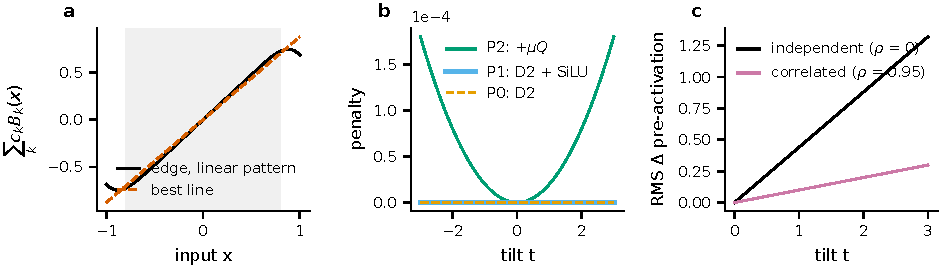
\includegraphics[width=\linewidth]{fig1_mechanism.pdf}
  % CAPTION-DRAFT: review (numbers from paper2/figures/fig1_mechanism.json)
  \caption{Mechanism (computed illustration) for the edge type of Section~\ref{sec:2} (8 Gaussian RBFs on $[-1, 1]$). \textbf{(a)} Edge function produced by a unit linear coefficient pattern and its best straight line; the shaded band is the central 80\% of the range, where the maximum deviation is 2.0\% of the function's range (12.9\% over the full range). \textbf{(b)} Penalty as a function of a tilt $t$ applied as $+t$ to edge 1 and $-t$ to edge 2: the second-difference penalty (P0) and P1 are exactly zero for every $t$; only P2's term $\mu Q$ grows ($\lambda = 0.001$, $\mu = 1e-05$). \textbf{(c)} RMS change in the unit's pre-activation per unit tilt: 0.0996 on correlated inputs ($\rho = 0.95$) against 0.4403 on independent inputs (4.42$\times$).}
  \label{fig:mechanism}
\end{figure}

\textbf{Step 3: no finite minimum.} "Nearly free" is not "free". Moving along it lets the model shed curvature into the free affine and SiLU components, so the loss decreases monotonically along the direction. Both terms contribute (post-hoc decomposition). In the synthetic runaway models the smoothness penalty fell to about a quarter of its early value and supplied a median 61\% of the decrease, while training error fell only 5\%. On real data, from early stopping to the capped state, the penalty fell 8--88$\times$ but supplied 17--36\% of the decrease, the data term the rest. In both, the growth went into whatever the penalty left free: the linear part of the RBF coefficients grew 34--40$\times$ in the synthetic runaway cells, and the SiLU weights 85$\times$ where they were unpenalised. In 12 of 20 synthetic runaway models, training error fell while test error rose. The infimum lies at infinity: gradients stay small but non-zero, the parameter norm grows without bound, and no minimum can be certified. Different seeds drift along different such directions.

\textbf{Step 4: any layer can be affected.} The argument needs only correlated inputs to a layer. Hidden units can become correlated during training, and then the output layer can host the same runaway even when the raw inputs are independent. Correlated hidden units appear necessary for this but not sufficient: they also occur in models that converge once the null space is penalised. Section 4 shows both forms.

\textbf{Consequences.}

\begin{itemize}
  \item \textbf{Non-identifiability:} edges differ across seeds by large affine components that leave predictions almost unchanged.
  \item \textbf{Non-convergence:} second-order optimisers stall; certification criteria fail.
  \item \textbf{Extrapolation risk:} off the training correlation pattern, $x_1 - x_2$ is no longer small, and the inflated components stop cancelling.
\end{itemize}

\textbf{The fix.} Penalise the null space directly. For each edge, let $P_{\mathrm{null}}$ project its RBF coefficients onto constant-plus-linear patterns in the centre index, and add

\begin{equation}
  Q = \sum_{e} \lVert P_{\mathrm{null}}\, c_e \rVert^{2}
\end{equation}

with a small weight $\mu$, in addition to a penalty on the SiLU weight. This makes every affine component cost something, which turns the infinite descent into a finite minimum.

\section{Controlled study}\label{sec:4}

\textbf{Design.} A teacher KAN [4, 3, 1] with smooth, hand-specified edges (fitted by smoothness-penalised least squares) generates targets with Gaussian noise of 5\% of the output spread; n = 2000 training rows. Inputs are $\mathcal{N}(0, 1)/3$, clipped to the grid, either independent or correlated in pairs ($\rho$ = 0.95 for $x_1/x_2$ and $x_3/x_4$). Students share the teacher's architecture and are trained under three penalty levels:

\begin{itemize}
  \item \textbf{P0:} second-difference penalty on RBF coefficients ($\lambda$ = $10^{-3}$).
  \item \textbf{P1:} P0 plus $K_{\mathrm{silu}}\,\alpha^{2}$ on each SiLU weight (Bagrow-style curvature penalty, $K_{\mathrm{silu}}$ = 0.443).
  \item \textbf{P2:} P1 plus $\mu Q$, the affine null-space penalty.
\end{itemize}

Each of the 6 cells has 8 seeds. Each student is trained with AdamW and early stopping, then polished with an exact-Hessian trust-region method and certified by a second-order criterion (gradient, curvature and Newton decrement). $\mu$ was calibrated before the experiment by a pre-registered rule: $10^{-6}$ failed the pilot (5.0$\times$ growth) and $10^{-5}$ passed (1.32$\times$) and was frozen.

\textbf{The teacher itself runs away.} Polished under P0 and P1 on correlated inputs, the teacher's parameters grew 85$\times$ and 1069$\times$ without certifying, while its predictions stayed within half a noise standard deviation of the original. The runaway changes the parameters, not the function.

\begin{table}[t]
  \centering
  % CAPTION-DRAFT: review
  \caption{Synthetic $2\times3$ study, per cell.}
  \label{tab:synthetic}
  \small
  \begin{tabular}{lp{0.2\linewidth}p{0.2\linewidth}p{0.2\linewidth}p{0.2\linewidth}p{0.2\linewidth}p{0.2\linewidth}p{0.2\linewidth}p{0.2\linewidth}p{0.2\linewidth}p{0.2\linewidth}p{0.2\linewidth}p{0.2\linewidth}p{0.2\linewidth}p{0.2\linewidth}p{0.2\linewidth}p{0.2\linewidth}p{0.2\linewidth}p{0.2\linewidth}p{0.2\linewidth}p{0.2\linewidth}p{0.2\linewidth}p{0.2\linewidth}p{0.2\linewidth}p{0.2\linewidth}p{0.2\linewidth}p{0.2\linewidth}p{0.2\linewidth}p{0.2\linewidth}p{0.2\linewidth}p{0.2\linewidth}p{0.2\linewidth}p{0.2\linewidth}p{0.2\linewidth}p{0.2\linewidth}p{0.2\linewidth}p{0.2\linewidth}p{0.2\linewidth}p{0.2\linewidth}p{0.2\linewidth}p{0.2\linewidth}p{0.2\linewidth}p{0.2\linewidth}p{0.2\linewidth}p{0.2\linewidth}p{0.2\linewidth}p{0.2\linewidth}p{0.2\linewidth}p{0.2\linewidth}p{0.2\linewidth}p{0.2\linewidth}p{0.2\linewidth}p{0.2\linewidth}p{0.2\linewidth}p{0.2\linewidth}p{0.2\linewidth}p{0.2\linewidth}p{0.2\linewidth}p{0.2\linewidth}p{0.2\linewidth}}
  \toprule
  Cell & Norm growth & Certified & Unit match to reference \\
  \midrule
  Independent, P0 & 12.5$\times$ & 6/8 & 1.000 \\
  Independent, P1 & 7.9$\times$ & 6/8 & 1.000 \\
  Independent, P2 & 1.09$\times$ & 8/8 & 1.000 \\
  Correlated, P0 & 65.7$\times$ & 0/8 & 0.774 \\
  Correlated, P1 & 32.1$\times$ & 0/8 & 0.883 \\
  Correlated, P2 & 1.00$\times$ & 8/8 & 1.000 \\
  \bottomrule
  \end{tabular}
\end{table}

Medians over 8 seeds; growth is the squared parameter norm, polished over early-stopped.

\textbf{Results.}

\begin{itemize}
  \item \textbf{The published-style penalty does not prevent the runaway.} Penalising the SiLU weight (P1) halved the growth on correlated inputs but left 0 of 8 models certified (Figure~\ref{fig:synthetic}).
  \item \textbf{Closing the null space prevents it everywhere.} P2 gave 16 of 16 certified models with no growth, in both input conditions.
  \item \textbf{Without the runaway, the internals are recoverable.} Every cell without a runaway matched the reference's units and edges exactly (1.000), with seed-to-seed differences around $10^{-4}$.
  \item \textbf{Independent inputs are not fully safe.} Under P0 and P1, most independent seeds grew substantially (8--12$\times$) but settled at certified minima; 4 of 16 (seeds 0 and 4 in each cell) never certified.
\end{itemize}


\begin{figure}[t]
  \centering
  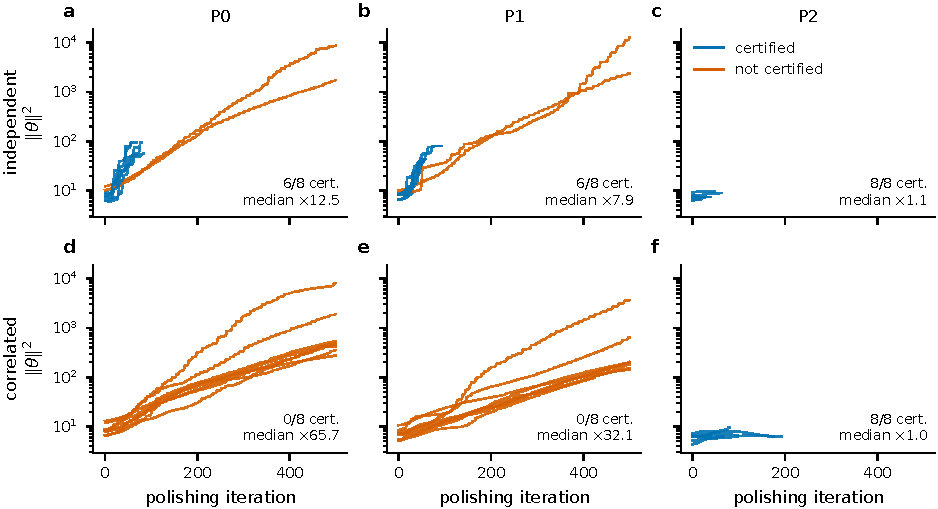
\includegraphics[width=\linewidth]{fig2_synthetic.pdf}
  % CAPTION-DRAFT: review (numbers from paper2/figures/fig2_synthetic.json)
  \caption{Synthetic $2\times3$ study: $\|\theta\|^2$ over trust-exact polishing iterations (log scale), one line per seed, coloured certified (blue) or not certified (vermillion). Rows: independent and correlated inputs; columns: P0, P1, P2. Per panel, certified seeds and median growth (polished over early-stopped): independent P0: 6/8 certified, $\times$12.5; independent P1: 6/8 certified, $\times$7.9; independent P2: 8/8 certified, $\times$1.1; correlated P0: 0/8 certified, $\times$65.7; correlated P1: 0/8 certified, $\times$32.1; correlated P2: 8/8 certified, $\times$1.0.}
  \label{fig:synthetic}
\end{figure}

\textbf{Where the runaway lives.} A post-hoc anatomy of the parameter change shows that in the correlated cells almost all growth sits in the output layer: the layer-1 share of the change was 0.110 (P0) and 0.024 (P1) (Figure~\ref{fig:where}a). It went into the affine part of the output edges' RBF coefficients and, under P0, into their SiLU weights. Cancellation across the edges entering the output rose from about 1.9 to 3.1--3.2, and no hidden unit saturated. The two uncertified independent-P0 seeds put 99.4\% of their change into the output layer. This is Step 4 of Section 3. Among independent-input models, those that ran away were exactly those whose hidden units had become correlated (largest pairwise correlation 0.70, against 0.05 for certified models; Figure~\ref{fig:where}b), while certified P2 models kept correlations up to 0.88 without running away (post-hoc).


\begin{figure}[t]
  \centering
  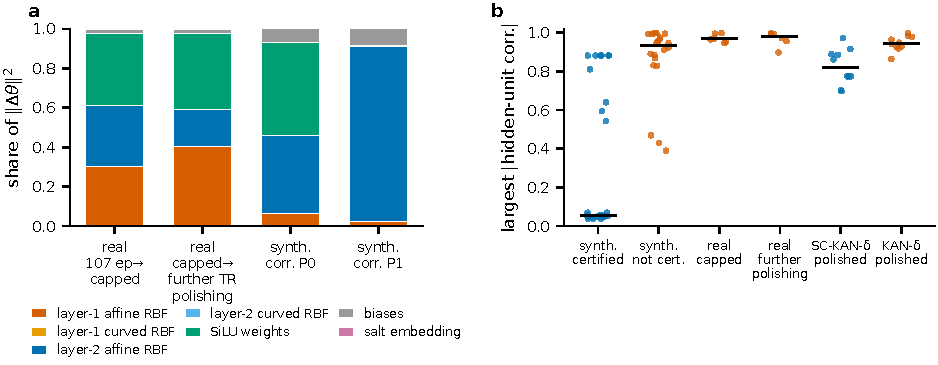
\includegraphics[width=\linewidth]{fig4_where.pdf}
  % CAPTION-DRAFT: review (numbers from paper2/figures/fig4_where.json)
  \caption{Where the runaway lives. \textbf{(a)} Mean share of $\|\Delta\theta\|^2$ by parameter block. Real data, 107 epochs$\to$capped: layer-1 affine RBF 0.30, layer-2 affine RBF 0.31, SiLU weights 0.37; capped$\to$Part~A: 0.40, 0.19, 0.38; synthetic correlated P0: layer-2 affine RBF 0.39, SiLU weights 0.47; correlated P1: layer-2 affine RBF 0.89. The real-data split was evaluated post hoc from archived weights (Appendix~\ref{app:repro}). \textbf{(b)} Largest absolute correlation between hidden-unit activations on the training rows, median: synth. certified 0.054 ($n=28$); synth. not cert. 0.935 ($n=20$); real capped 0.968 ($n=6$); real Part A 0.983 ($n=6$); SC-KAN-$\delta$ polished 0.818 ($n=10$); KAN-$\delta$ polished 0.946 ($n=10$). Blue: certified; vermillion: not certified or runaway.}
  \label{fig:where}
\end{figure}

\textbf{Verdicts.} Of six pre-registered predictions, one held (the certification pattern, X2) and five failed. The failures refine rather than contradict the mechanism. Independent cells exceeded the growth threshold, mostly through finite growth. Cancellation and extrapolation effects were weaker than predicted. Recoverability failed only because the runaway cells were more recoverable than predicted, not less. In this synthetic setting, polishing did not degrade extrapolation: most of the off-pattern error in correlated cells was present at early stopping.

\section{Real-data case study: electrolyte conductivity}\label{sec:5}

\textbf{Task and model.} The CALiSol-23 challenge \citep{deblasio2024calisol} asks for the log conductivity of lithium-ion electrolytes; every test sample contains diethyl carbonate (DEC), which never appears in training. KAN-delta anchors each prediction on the measured conductivity of pure propylene carbonate (PC) and learns only the correction, $\log k = \log k_{\mathrm{PC}} + x_{\mathrm{co}}\, h(z)$, where h is a FastKAN-style network of shape [10, 6, 1]. Its inputs are physical descriptors of the solvents (dielectric constant, log viscosity, molar mass), temperature, molality and a salt embedding. A second-difference penalty acts on the RBF coefficients, and the SiLU weights are unpenalised. Early-stopped after 107 AdamW epochs, it reached RMSE 0.142 on a held-out co-solvent.

\textbf{The inputs are correlated and few-valued.} The three co-solvent descriptors take only 30 distinct combinations in training, and dielectric constant and log viscosity correlate at r = 0.966.

\textbf{Nothing ever converged.}

\begin{itemize}
  \item Of 190 pairs of polished independent seeds, none computed the same function.
  \item After 20,000 float64 L-BFGS iterations, 0 of 26 models converged; exact-Hessian trust-region methods also failed on every seed.
  \item Students trained on a frozen teacher matched its predictions (correlation 0.9988) but not its hidden units (0.66).
\end{itemize}

\textbf{The anatomy matches Section 3.}

\begin{itemize}
  \item From early stopping to the capped state, the squared parameter norm grew 150--1550$\times$ while the smoothness penalty fell 8--88$\times$.
  \item At least 99.9\% of the coefficient change during exact-Newton polishing lay in the penalty's affine null space, in 9 of 9 models.
  \item Cancellation within an edge (SiLU against RBF) stayed small, 1.13--1.33. Cancellation across the edges entering a unit rose from 1.7--2.9 to 4--10, consistent with the correlated descriptors.
  \item The runaway spread across both layers: 30--40\% of the parameter change went into layer-1 affine RBF coefficients, 37--38\% into SiLU weights and 19--31\% into layer-2 affine coefficients (post-hoc), and 12--39\% of hidden units saturated. In the synthetic runaway the output layer dominated.
\end{itemize}

\textbf{Extrapolation suffered.} Polishing beyond early stopping, under a weak null-space penalty, raised the held-out RMSE from 0.142 to 1.03. The cancelling components appear to stop cancelling on the unseen co-solvent, whose descriptors sit off the training correlation pattern. This degradation was much stronger than in the synthetic study, where correlation itself caused most of the off-pattern error; the real model was larger, its norms grew further, and the test solvent lay at the edge of the descriptor range.

\section{Closing the blind spot, and what remains}\label{sec:6}

\textbf{Dose-response on real data.} Adding $\mu Q$ (with the SiLU weights included in Q) and polishing from the early-stopped weights:

\begin{table}[t]
  \centering
  % CAPTION-DRAFT: review
  \caption{Dose-response in $\mu$ on real data (seeds).}
  \label{tab:dose}
  \small
  \begin{tabular}{l l p{0.18\linewidth} l p{0.16\linewidth}}
  \toprule
  $\mu$ & Seeds at a numerical minimum & Negative curvature (seeds) & Norm growth (seeds) & Training fit vs runaway \\
  \midrule
  $10^{-6}$ & 0 of 6 & up to 9 eigenvalues & 21--31$\times$ & about equal \\
  $10^{-5}$ & 4 of 6 & up to 4 eigenvalues & 9--43$\times$ & 12--22\% worse \\
  $10^{-4}$ & 6 of 6 & none & 1.6--16$\times$ & 15--39\% worse \\
  \bottomrule
  \end{tabular}
\end{table}

Under a second-order certificate, all six seeds at $\mu$ = $10^{-4}$ were certified (Figure~\ref{fig:dose}). (The originally pre-registered criterion, which required 10 stationary iterations, proved unreachable because the optimiser stops a few iterations after reaching a minimum; the certificate was defined afterwards and is reported alongside the original verdict.) Saturation fell to at most 0.5\% and cross-edge cancellation to 2.2--2.9.


\begin{figure}[t]
  \centering
  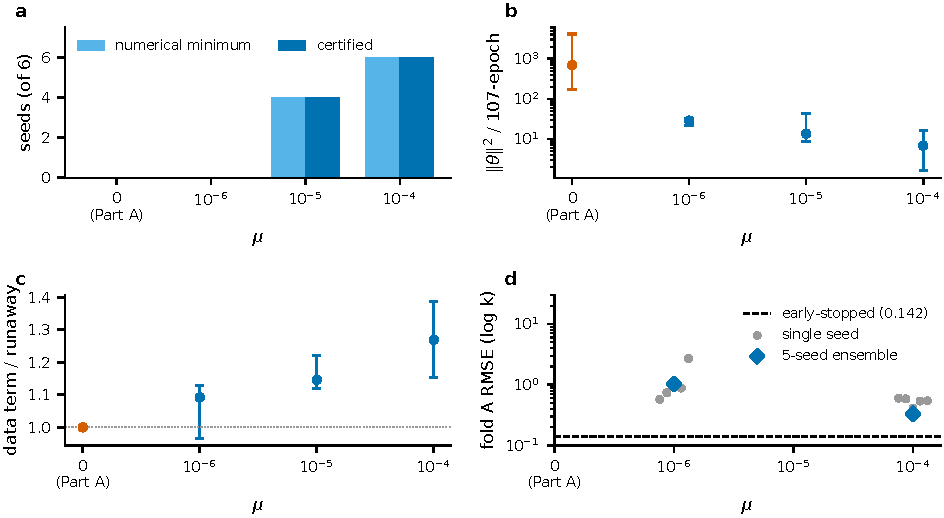
\includegraphics[width=\linewidth]{fig3_dose_response.pdf}
  % CAPTION-DRAFT: review (numbers from paper2/figures/fig3_dose_response.json)
  \caption{Real-data dose-response in the null-space weight $\mu$ (6 KAN-delta seeds; $\mu = 0$ is the runaway reference, stage-2 Part~A). \textbf{(a)} Seeds at a numerical minimum / certified: 0: 0/0; 1e-06: 0/0; 1e-05: 4/4; 0.0001: 6/6. \textbf{(b)} $\|\theta\|^2$ relative to the 107-epoch state, median (range): 0: 690.0 (170.0--4145.5); 1e-06: 28.8 (21.2--31.5); 1e-05: 13.6 (8.6--43.1); 0.0001: 6.8 (1.6--16.0). \textbf{(c)} Training data term relative to the runaway, median: 1e-06: 1.092; 1e-05: 1.146; 0.0001: 1.269. \textbf{(d)} Fold A RMSE: early-stopped 0.142 (dashed line); polished 5-seed ensemble 1.026 at $\mu = 10^{-6}$ and 0.334 at $\mu = 10^{-4}$; grey points are single seeds.}
  \label{fig:dose}
\end{figure}

\textbf{A known solution becomes recoverable.} Under the regularised loss, the original teacher is no longer a minimum. Optimising it under the same loss gives a "regularised teacher" computing nearly the same function (correlation 0.9992). Students match its units at 0.87--0.90 and its edges at 0.97--0.98, against 0.68--0.72 and 0.84--0.91 for the original teacher. This comparison was defined after the results and is exploratory.

\textbf{The penalty acts partly as gauge fixing.} At the certified minima, the layer-2 constant shift, an essentially exact symmetry, owes 96\% of its curvature to $\mu Q$: the regulariser selects one representative. The layer-1 constant shift (46\%) and unit rescaling (24\%) are only approximate symmetries in this architecture, because Gaussian bumps cannot represent constants exactly and tanh breaks rescaling.

\textbf{Convergence is not uniqueness.} Independent seeds at certified minima still disagreed: their median prediction difference fell by only 26\% (Figure~\ref{fig:uniqueness}b). With the runaway removed, the loss has several distinct isolated minima.


\begin{figure}[t]
  \centering
  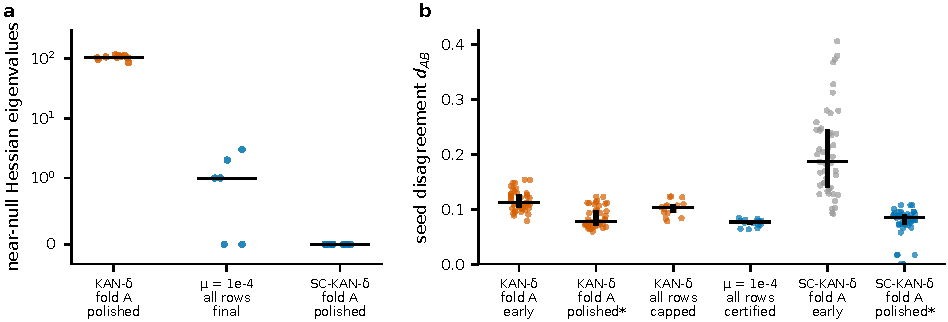
\includegraphics[width=\linewidth]{fig5_uniqueness.pdf}
  % CAPTION-DRAFT: review (numbers from paper2/figures/fig5_uniqueness.json)
  \caption{Convergence is not uniqueness. \textbf{(a)} Near-null Hessian eigenvalues ($|\lambda| < 10^{-8}\lambda_{\max}$) at the end of polishing: KAN-delta baseline on fold A, median 106 (range 86--116); null-space penalty $\mu = 10^{-4}$ on all rows, median 1 (range 0--3); SC-KAN-delta on fold A, 0--0. \textbf{The baseline counts are taken at non-stationary points}: none of the 10 baseline models was certified, and all stopped at the 500-iteration cap. \textbf{(b)} Seed disagreement $d_{AB}$ (median, interquartile range): KAN-$\delta$ fold A early 0.112; KAN-$\delta$ fold A polished$^*$ 0.077; KAN-$\delta$ all rows capped 0.104; $\mu$ = 1e-4 all rows certified 0.077; SC-KAN-$\delta$ fold A early 0.187; SC-KAN-$\delta$ fold A polished$^*$ 0.085. Groups marked $^*$ (polished fold A) are not in any committed result: they were evaluated post hoc from the archived polished weights (SHA-verified; predictions on the 1434 fold A training rows), without any re-optimisation.}
  \label{fig:uniqueness}
\end{figure}

\textbf{Extrapolation.} On the held-out co-solvent, RMSE was 0.142 for the early-stopped model, 1.026 after polishing at $\mu$ = $10^{-6}$ and 0.33 at $\mu$ = $10^{-4}$. Bounding the runaway recovers most of the damage, but early stopping remains the most accurate choice.

\textbf{Structured alternatives.} We tested two architectures designed to remove runaway routes by construction, against the early-stopped baseline, with leave-one-co-solvent-out (LOCO) validation:

\begin{table}[t]
  \centering
  % CAPTION-DRAFT: review
  \caption{Structured alternatives against the early-stopped baseline.}
  \label{tab:alternatives}
  \small
  \begin{tabular}{l p{0.24\linewidth} l l p{0.16\linewidth}}
  \toprule
  Model & Idea & LOCO RMSE & Converged & Seed agreement \\
  \midrule
  Baseline KAN-delta & As above & 0.255 & 0/10 & 0.112 \\
  Shared-curve KAN & One curve per input, mixed by penalised weights & 0.292 & 10/10 & 0.187 early; 0.085 polished \\
  Two-anchor excess model & Pure-solvent offset plus $x(1 - x)$ mixing term & 0.283 & not tested & not tested \\
  \bottomrule
  \end{tabular}
\end{table}

Seed agreement is the median prediction difference between seeds (lower is better). The shared-curve model converged every time, ending with no near-flat directions where the baseline had a median of 106 (range 86--116, at non-stationary points; Figure~\ref{fig:uniqueness}a), and it was less accurate. At the early-stopped state its seeds agreed less than the baseline's (the pre-registered comparison); after polishing to certified minima their median disagreement fell to 0.085, with some seed pairs reaching the same minimum (post-hoc). The excess model's "pure co-solvent offset" tracked viscosity rather than dielectric constant (rank correlation $-$0.85, post hoc), reflecting that no training row contains a pure co-solvent.

\section{Recommendations for practitioners}\label{sec:7}

\begin{enumerate}
  \item \textbf{Penalise the affine null space and the SiLU weights.} If a KAN uses a second-difference or curvature penalty, add a small penalty on the constant-plus-linear component of each edge's coefficients and on each SiLU weight, in every layer. Calibrate its weight so it barely moves a known smooth solution.
  \item \textbf{Check input correlations, including between hidden units.} Strongly correlated or few-valued inputs make the first layer vulnerable; any hidden layer can expose the next one.
  \item \textbf{Monitor parameter norms, not only the loss.} Steady norm growth with a slowly falling loss and stubborn gradients is the signature of the runaway. Certify convergence with a second-order criterion rather than assuming it.
  \item \textbf{Do not read edges from unconverged models.} Compare edges across seeds only after removing exact gauge freedoms, and only for models that reached certified minima.
  \item \textbf{Treat seed disagreement as information.} Even at certified minima, distinct solutions can remain. Disagreement then signals that the data do not determine the function, not merely that training was unfinished.
  \item \textbf{Validate on genuinely new conditions.} A held-out fold from the training distribution can understate extrapolation error severalfold; leave-one-group-out validation is closer to the use case.
  \item \textbf{Keep early stopping as a baseline.} In our real-data case it gave the best held-out accuracy of every variant tested.
\end{enumerate}

\section{Limitations and research process}\label{sec:8}

\textbf{Scope.}

\begin{itemize}
  \item One real dataset and one synthetic teacher; small networks ([4, 3, 1] and [10, 6, 1]).
  \item One edge type: Gaussian RBFs on fixed centres with a SiLU base. The argument applies to B-spline KANs with second-difference or curvature penalties, but we did not test them directly.
  \item Our P1 keeps the second-difference penalty on RBF coefficients and adds Bagrow's SiLU term; it is Bagrow-style, not a replication of his RBF curvature form.
  \item The null-space weight used in the shared-curve model was carried over from the synthetic calibration, not re-calibrated.
\end{itemize}

\textbf{Post-hoc elements.} The second-order certificate, the regularised-teacher comparison, the gauge-curvature analysis and both anatomy studies were defined after seeing results. We report them as exploratory and never in place of pre-registered verdicts.

\textbf{Extrapolation.} The strong degradation from polishing appeared on real data but not in the synthetic study, so we do not claim it as a general law.

\textbf{Process.} Each study committed its predictions, thresholds and interpretation rules before its code existed; any later change was dated and recorded as an amendment, and every verdict is linked to the commit that produced it. Several predictions failed or proved untestable as specified; following them up, rather than reinterpreting them, is what led to the mechanism reported here. Experiments were run with an AI coding agent working under this protocol, with a rule that committed files take precedence over any number stated in a prompt.


\bibliography{references}
\bibliographystyle{tmlr}

\appendix
\ifdefined\PREPRINT
  % GENERATED by build_tex.py (preprint: real commit hashes)
\section{All pre-registered predictions}\label{app:prereg}

Generated by \texttt{paper2/tex/build\_tex.py} from the committed verdict sections; the cell text is the committed wording. Each study opens with its pre-registration's title and its committed question (or theory). Commits are given as pre-registration $\to$ results (in the anonymous version, as neutral labels S-NN). Thresholds are part of each prediction's wording.

\subsection{Synthetic controlled study}
\noindent\textit{Pre-registration:} ``Pre-registration: synthetic teacher-student test of the runaway mechanism (paper2/synth)''. \textbf{Teacher and students: KAN [4, 3, 1].} Two stacked \texttt{kan.KANLayer}s with tanh between them, as in \texttt{kan.KAN}, but \textbf{without} the salt embedding that \texttt{kan.KAN} always adds. Same edge type: SiLU base plus 8 Gaussian RBFs on fixed centres linspace($-$1, 1, 8), width 2/7.

{\footnotesize\setlength{\tabcolsep}{3pt}
\begin{longtable}{R{0.07\linewidth} R{0.28\linewidth} R{0.35\linewidth} R{0.09\linewidth} R{0.11\linewidth}}
\toprule
ID & Prediction (threshold) & Result & Verdict & Commits \\
\midrule
\endhead
X1 & runaway ($\geq$ 10) in correlated P0 and P1; $\leq$ 3 in the three independent cells and correlated P2 & Correlated P0 $\times$65.7 and P1 $\times$32.1, and P2 $\times$1.00, as predicted. \textbf{But independent P0 $\times$12.5 and P1 $\times$7.9 exceed 3} (independent P2 $\times$1.09) & \textbf{failed} & dfd281d$\to$\allowbreak 34cc321 \\
X2 & certified $\leq$ 2/8 in correlated P0 and P1; $\geq$ 6/8 elsewhere & correlated P0 0/8, P1 0/8; independent 6/8, 6/8, 8/8; correlated P2 8/8 & \textbf{held} & dfd281d$\to$\allowbreak 34cc321 \\
X3 & cancellation in correlated P0 and P1 each $\geq$ 2 $\times$ correlated P2 & P0 3.29 and P1 2.32, against 2 $\times$ 1.99 = 3.98 & \textbf{failed} & dfd281d$\to$\allowbreak 34cc321 \\
X4 & off-manifold ratio $\geq$ 3 in correlated P0 and P1, $\leq$ 1.5 in P2 & P0 1.22, P1 \textbf{0.77}; P2 0.78 (the P2 part held) & \textbf{failed} & dfd281d$\to$\allowbreak 34cc321 \\
X5 & Spearman(cancellation, off-manifold RMSE) $\geq$ 0.6 over the 24 correlated models & $\rho$ = +0.177, p = 0.407 & \textbf{failed} & dfd281d$\to$\allowbreak 34cc321 \\
X6 & unit match $\geq$ 0.85 in the independent cells and correlated P2; < 0.7 in correlated P0 and P1 & The first part held: 1.000 in all four no-runaway-predicted cells. \textbf{The second part failed: correlated P0 0.774 and P1 0.883 are not < 0.7} & \textbf{failed} & dfd281d$\to$\allowbreak 34cc321 \\
\bottomrule
\end{longtable}}
\subsection{Real-data case study}
\noindent\textit{From the case-study close-out:} KAN-$\delta$ predicts Li-electrolyte conductivity for the CALiSol-23 DEC holdout. Its
prediction is log k = a measured pure-PC anchor + x\_co $\cdot$ h(solvent descriptors, 1/T, molality, salt).
Its first layer is a [8 continuous inputs + 2 salt-embedding, 6, 1] FastKAN, with SiLU + 8 Gaussian
RBFs per edge and a smoothness penalty (\texttt{kan.py}, \texttt{final.py}).

Rows are as committed in the case-study summary (one row may cover several predictions, e.g.\ F2--F5). The rank intervention's verdicts are given per arm in the result column.

{\footnotesize\setlength{\tabcolsep}{3pt}
\begin{longtable}{R{0.14\linewidth} R{0.26\linewidth} R{0.29\linewidth} R{0.10\linewidth} R{0.11\linewidth}}
\toprule
Study & Prediction (threshold) & Result & Verdict & Commits \\
\midrule
\endhead
Gauge study & \textbf{Control 1}: teacher edges recovered, median dense corr $\geq$ 0.8 & 0.301 (sanity: h corr 0.913 < 0.95) & \textbf{failed} & c11dd92$\to$\allowbreak{}e68e2eb \\
Gauge study & P1: gauge fixing removes $\geq$ 50\% of edge variance & not run & inconclusive (gated by Control 1) & c11dd92$\to$\allowbreak{}e68e2eb \\
Gauge study & P2: sparse $\geq$ 2$\times$ dense, DEC region highest & not run & inconclusive (gated) & c11dd92$\to$\allowbreak{}e68e2eb \\
Gauge study & P3: (e) < (d) < (c) < (a) & not run & inconclusive (gated) & c11dd92$\to$\allowbreak{}e68e2eb \\
Gauge study & P4: every seed has a unit with |corr| < 0.8 & not run & inconclusive (gated) & c11dd92$\to$\allowbreak{}e68e2eb \\
Gauge study & P5: KAN-full edge variance > KAN-$\delta$ & not run & inconclusive (gated) & c11dd92$\to$\allowbreak{}e68e2eb \\
Gauge study & P6: seed spread flags errors & Spearman +0.169 (A) / +0.213 (B); fold B RMSE at 80\% coverage 0.153 vs random 0.137 & \textbf{failed} & c11dd92$\to$\allowbreak{}67fe9f2 \\
Control 2 & C1: (I,C) edges $\geq$ 0.9 and units $\geq$ 0.9 & prediction corr 0.947 < 0.99 & inconclusive (gate failed) & 45b336f$\to$\allowbreak{}a260aef \\
Control 2 & C2: (R,C) invT, molal $\geq$ 0.9; co-solvent < 0.7 & prediction corr 0.969 < 0.99 & inconclusive (gate failed) & 45b336f$\to$\allowbreak{}a260aef \\
Control 2 & C3: 107 epochs gives prediction corr < 0.95 & 0.858 (I,S), 0.919 (R,S) & \textbf{held} & 45b336f$\to$\allowbreak{}a260aef \\
Control 3 & C1': (I) passes the gate, edges $\geq$ 0.9, units $\geq$ 0.9 & (I) RMSE/std 0.128 > 0.05; unit match 0.648 & \textbf{failed} & 812a0fa$\to$\allowbreak{}9f59d39 \\
Control 3 & C2': (R) edges $\leq$ (I) edges $-$ 0.10 & (R) edges 0.852, units 0.659 & inconclusive ((I) failed the gate) & 812a0fa$\to$\allowbreak{}9f59d39 \\
Control 3 & C4: every continuous input $\geq$ 0.9 in (I) & -- & inconclusive ((I) failed the gate) & 812a0fa$\to$\allowbreak{}9f59d39 \\
Fiber & F1: $\geq$ 50\% of seed pairs on-fiber & 0/190 (closest d = 0.146) & \textbf{failed} & e83df2e$\to$\allowbreak{}f220a2f \\
Fiber & F2--F5 & not run & inconclusive (no on-fiber pairs) & e83df2e$\to$\allowbreak{}f220a2f \\
Fiber 2 & G1: $\geq$ 4/6 seeds and $\geq$ 10/20 students certify convergence & 0/6, 0/20 (all at the 20,000-iteration cap) & \textbf{failed} & 4af5250$\to$\allowbreak{}98eca9d \\
Fiber 2 & G2--G5 & not run & inconclusive (no converged model) & 4af5250$\to$\allowbreak{}98eca9d \\
Support & H1: dim(N) $\geq$ 5 & dim(N) = 36 of 72 & \textbf{held} & b473232$\to$\allowbreak{}c5505e5 \\
Support & H2: $\geq$ 50\% of N is REDISTRIBUTION within the correlated group & 18/36 & \textbf{held, exactly at threshold} & b473232$\to$\allowbreak{}c5505e5 \\
Support & H3: set A fraction in N $\geq$ 0.5 and $\geq$ 3$\times$ random & median 0.942 (random 0.5) & inconclusive (untestable: 3 $\times$ 0.5 > 1) & b473232$\to$\allowbreak{}c5505e5 \\
Support & H4: set B (capped), same criterion & median 0.949 & inconclusive (untestable) & b473232$\to$\allowbreak{}c5505e5 \\
Support & H5: flattest Hessian directions overlap N $\geq$ 0.5 & median 0.885; median layer-1 block share only 0.08 & \textbf{held}, with caveat (see \texttt{support\_\allowbreak{}prereg.md}) & b473232$\to$\allowbreak{}c5505e5 \\
Support & H6: fraction in N rises from control-3 to capped state, $\geq$ 15/20 & 20/20 (0.713 $\to$\allowbreak{} 0.949) & \textbf{held} & b473232$\to$\allowbreak{}c5505e5 \\
Rule & I1--I5 (gate) & 0 columns removed; gate stopped & inconclusive & 6c93bf4$\to$\allowbreak a53cc2a \\
Rank & I1: median max|grad| $\leq$ 0.1 $\times$ baseline & arm G: \textbf{failed} (4.00$\times$); arm F: \textbf{failed} (29.1$\times$) & see result & df44ead$\to$\allowbreak aeb6f87 \\
Rank & I2: median d\_AB $\leq$ 0.5 $\times$ baseline & arm G: \textbf{failed} (0.945$\times$); arm F: \textbf{failed} (0.808$\times$) & see result & df44ead$\to$\allowbreak aeb6f87 \\
Rank & I3 (sanity): median loss $\leq$ 1.10 $\times$ baseline & arm G: passed (1.004$\times$); arm F: passed, narrowly (1.099$\times$) & see result & df44ead$\to$\allowbreak aeb6f87 \\
Rank & I4: fold A RMSE $\leq$ 0.150 (KAN-$\delta$ 0.1420) & arm G: \textbf{held}, narrowly (0.1499); arm F: \textbf{failed} (0.1587) & see result & df44ead$\to$\allowbreak aeb6f87 \\
Rank & I5: edge corr on 1000/T and molality $\geq$ baseline + 0.1 (baseline 0.102) & arm G: \textbf{held} (0.927); arm F: \textbf{held} (0.338) & see result & df44ead$\to$\allowbreak aeb6f87 \\
Rank & I6: arm F's improvement $\geq$ arm G's in both I1 and I2 & arm G: \textbf{failed} (max|grad| 29.1$\times$ vs 4.00$\times$; d\_AB does favour F, 0.808 vs 0.945) & see result & df44ead$\to$\allowbreak aeb6f87 \\
Trust & T1 / T2: trust-krylov certifies $\geq$ 4/6 seeds / $\geq$ 2/3 students & 0/6, 0/3. All 9 stopped on scipy's "bad approximation" after 1--62 iterations; the Hessian was accurate to $\leq$ $2\times10^{-7}$ & \textbf{failed} & a77e8b4$\to$\allowbreak 67586d6 \\
Trust & T3--T5 & nothing converged & inconclusive & a77e8b4$\to$\allowbreak 67586d6 \\
Stage 2 & U1: trust-exact (exact Hessian, 500 iterations) certifies $\geq$ 4/6 seeds & 0/6. All 9 hit the iteration cap & \textbf{failed} & c6a9e83$\to$\allowbreak b8d6488 \\
Stage 2 & U2: with L2 $\lambda$ = $10^{-5}$, $\geq$ 4/6 seeds and $\geq$ 2/3 students & 1/6 seeds, 0/3 students & \textbf{failed} & c6a9e83$\to$\allowbreak b8d6488 \\
Stage 2 & U3: more converge at $10^{-5}$ than at $10^{-6}$ & 1 vs 0 & \textbf{held} & c6a9e83$\to$\allowbreak b8d6488 \\
Stage 2 & U4: converged L2 models' loss without L2 $\leq$ 1.05 $\times$ capped & 1.2545 & \textbf{failed} & c6a9e83$\to$\allowbreak b8d6488 \\
Stage 2 & U5: converged seeds' disagreement $\leq$ 0.5 $\times$ capped & only 1 converged & inconclusive & c6a9e83$\to$\allowbreak b8d6488 \\
Close & V1: at some $\mu$, $\geq$ 4/6 seeds and $\geq$ 2/3 students converge (stage2 criterion) & 0 certified at every $\mu$ & \textbf{failed} & e5105d7$\to$\allowbreak{}65ed55f \\
Close & V2: converged seeds' data term $\leq$ 1.05 $\times$ stage2 A & nothing certified at the selected $\mu$ = $10^{-6}$ & inconclusive & e5105d7$\to$\allowbreak{}65ed55f \\
Close & V3: $\|\theta\|^{2}$ $\leq$ 10 $\times$ start & same & inconclusive & e5105d7$\to$\allowbreak{}65ed55f \\
Close & V4: seed disagreement halved & same & inconclusive & e5105d7$\to$\allowbreak{}65ed55f \\
Close & V5: students' unit match $\geq$ 0.8 & same & inconclusive & e5105d7$\to$\allowbreak{}65ed55f \\
Close & V6: fold A RMSE $\leq$ 0.150 & 1.0262, bias +0.9028 & \textbf{failed} & e5105d7$\to$\allowbreak{}65ed55f \\
Certify & W1: at $\mu$ = $10^{-4}$, $\geq$ 5/6 seeds certified (second-order criterion, F-a) & 6/6; all 17 candidates certified & \textbf{held} & 5f4520a$\to$\allowbreak{}36f295b \\
Certify & W2: certified seeds' median d\_AB $\leq$ 0.5 $\times$ capped & 0.0771 vs capped 0.1041 ($-$26\%) & \textbf{failed} & 5f4520a$\to$\allowbreak{}36f295b \\
Certify & W3: certified students' unit match $\geq$ 0.8 (vs the original teacher) & 0.624 & \textbf{failed} & 5f4520a$\to$\allowbreak{}36f295b \\
Certify & W4: $\mu$ = $10^{-4}$ fold A RMSE $\leq$ 0.150 & 0.3345 & \textbf{failed} & 5f4520a$\to$\allowbreak{}36f295b \\
Certify & W5: $\mu$ = $10^{-4}$ fold A RMSE $\leq$ 0.5131 & 0.3345 & \textbf{held} & 5f4520a$\to$\allowbreak{}36f295b \\
Certify & W6: Spearman(cross-edge ratio, held-out RMSE) $\geq$ 0.6 & $\rho$ = +0.345, p = 0.328 (weak test) & \textbf{failed} & 5f4520a$\to$\allowbreak{}36f295b \\
\bottomrule
\end{longtable}}
\noindent Committed tally of the case study:

{\footnotesize\setlength{\tabcolsep}{3pt}
\begin{longtable}{R{0.55\linewidth} r r r}
\toprule
Study & Held & Failed & Inconclusive \\
\midrule
\endhead
First table (Control 1, P1--P6, C1--C3, C1'/C2'/C4, F1--F5, G1--G5, H1--H6) & 5 & 5 & 19 \\
Rule (I1--I5) & 0 & 0 & 5 \\
Rank (I1, I2, I4, I5 per arm, I6) & 3 & 6 & 0 \\
Trust (T1--T5) & 0 & 2 & 3 \\
Stage 2 (U1--U5) & 1 & 3 & 1 \\
Close (V1--V6) & 0 & 2 & 4 \\
Certify (W1--W6) & 2 & 4 & 0 \\
\textbf{Total} & \textbf{11} & \textbf{22} & \textbf{32} \\
\bottomrule
\end{longtable}}
\subsection{Shared-curve KAN}
\noindent\textit{Pre-registration:} ``SC-KAN-$\delta$ (shared-curve KAN-$\delta$): pre-registration''. \textbf{Inputs:} the 8 continuous final.py features (flag 11), scaled exactly as in final.py. Salt enters through a learned 2-number embedding e(salt), passed through tanh.

Run after the case-study close-out; not part of the 65 predictions above.

{\footnotesize\setlength{\tabcolsep}{3pt}
\begin{longtable}{R{0.07\linewidth} R{0.28\linewidth} R{0.35\linewidth} R{0.09\linewidth} R{0.11\linewidth}}
\toprule
ID & Prediction (threshold) & Result & Verdict & Commits \\
\midrule
\endhead
S1 & SC LOCO RMSE $\leq$ 1.05 $\times$ baseline & unweighted mean SC 0.2923 vs base 0.2554 (ratio 1.145; threshold 0.2681). Also reported: row-weighted 0.2478 / 0.2297 (1.079); folds $\geq$ 20 rows 0.3138 / 0.2093 (1.499) & failed & 0053d01$\to$\allowbreak e00e37f \\
S2 & SC fold A RMSE $\leq$ 0.160 & SC 0.1757 (base 0.1420) & failed & 0053d01$\to$\allowbreak e00e37f \\
S3 & SC median d\_AB $\leq$ 0.5 $\times$ baseline & SC 0.1865 vs base 0.1120 (threshold 0.0560): SC seeds agree \emph{less} than baseline seeds & failed & 0053d01$\to$\allowbreak e00e37f \\
S4 & curve corr $\geq$ 0.90 for $\geq$ 6 of 8 inputs & 3 of 8 (M\_co 0.959, mix\_lneta 0.970, invT 0.986); lowest x\_co 0.596; others 0.871--0.891 & failed & 0053d01$\to$\allowbreak e00e37f \\
S5 & $\geq$ 8/10 SC fold A models certified & SC 10/10 (max|grad| $\leq$ $7\times10^{-10}$, 0 near-null eigenvalues); baseline 0/10 (all hit the 500-iteration cap) & held & 0053d01$\to$\allowbreak e00e37f \\
S6 & median $\beta$-norm polished/early $\leq$ 3 (calibrated) & median 1.337 (range 0.652--2.356); $\|\theta\|^{2}$ $\times$4.59 (base $\times$67.9, range 30.6--281) & held & 0053d01$\to$\allowbreak e00e37f \\
S7 & SC polished/early fold A RMSE $\leq$ 1.5 & SC 1.920 (0.1757 $\to$\allowbreak{} 0.3373); baseline 5.736 (0.1420 $\to$\allowbreak{} 0.8147) & failed & 0053d01$\to$\allowbreak e00e37f \\
S8 & d log k/d(1000/T) < 0 on $\geq$ 95\% rows in $\geq$ 8/10 seeds & 10/10 (median share 1.000; 1424 rows, 10 excluded per D4) & held & 0053d01$\to$\allowbreak e00e37f \\
S9 & Spearman(1000/T, |slope|) > 0 in $\geq$ 8/10 seeds & 10/10 (median +0.661, range +0.406 to +0.885) & held & 0053d01$\to$\allowbreak e00e37f \\
S10 & d log k/d(ln $\eta$\_mix) < 0 on $\geq$ 90\% rows in $\geq$ 8/10 seeds & 7/10 (median share 0.967; s0 0.892, s2 0.892, s8 0.826) & failed & 0053d01$\to$\allowbreak e00e37f \\
\bottomrule
\end{longtable}}
\subsection{Two-anchor excess model}
\noindent\textit{Pre-registration:} ``EX-KAN (two-anchor excess model): pre-registration''. log k = anchor\_PC + x\_co $\cdot$ s(eps\_co, ln\_eta\_co, M\_co, 1000/T) + x\_co $\cdot$ (1 $-$ x\_co) $\cdot$ g(eps\_co, ln\_eta\_co, M\_co, 1000/T, molality, salt) So $\delta$ = log k $-$ anchor\_PC = x\_co $\cdot$ [s + (1 $-$ x\_co) $\cdot$ g].

Run after the case-study close-out; not part of the 65 predictions above.

{\footnotesize\setlength{\tabcolsep}{3pt}
\begin{longtable}{R{0.07\linewidth} R{0.28\linewidth} R{0.35\linewidth} R{0.09\linewidth} R{0.11\linewidth}}
\toprule
ID & Prediction (threshold) & Result & Verdict & Commits \\
\midrule
\endhead
E1 & EX LOCO $\leq$ 0.95 $\times$ KAN-$\delta$ & unweighted mean EX 0.2834 vs threshold 0.2426 (base 0.2554; ratio 1.110). Row-weighted 0.2363 / 0.2297 (1.029); folds $\geq$ 20 rows 0.2662 / 0.2093 (1.272). EX is better on EC (0.237 vs 0.256), Sulfolane, 3-Glyme, 2-Glyme and Toluene, and worse on 2-MeTHF, THF, Methylene chloride, DME and EA & failed & 3938f8f$\to$\allowbreak 579b58f \\
E2 & EX fold A $\leq$ 0.142 & EX 0.1502 (base this run 0.1420) & failed & 3938f8f$\to$\allowbreak 579b58f \\
E3 & s agrees across seeds (separable co-solvents, Amendment 1) & median pairwise corr +0.987 over EA, EC, Methylene chloride: a weak test with 3 values per seed, and Methylene chloride is marginal. Seed SD of s: EA 0.063 (0.39 $\times$ the spread across co-solvents, 0.159), EC 0.091 (0.57 $\times$), Methylene chloride 0.067 (0.42 $\times$). Secondary ($\leq$ 2 rule, 7 co-solvents): +0.869 & held & 3938f8f$\to$\allowbreak 579b58f \\
E4 & mean s(low $\varepsilon$) < mean s(EC, Sulfolane) in $\geq$ 8/10 seeds & 0/10: the ordering is reversed in every seed. Per high-$\varepsilon$ co-solvent: vs EC alone 0/10 (EC median s +0.104), vs Sulfolane alone 0/10 (median $-$0.124). The low-$\varepsilon$ mean is +0.19 to +0.49 per seed. Sulfolane does not drive the failure on its own: EC alone fails in every seed too & failed & 3938f8f$\to$\allowbreak 579b58f \\
E5 & median seed-SD flagged $\geq$ 2 $\times$ separable (Amendment 1) & 0.091 vs 0.067, ratio 1.37. Secondary ($\leq$ 2 rule): 0.222 vs 0.069, ratio 3.22, no verdict; the secondary is driven by 3-Glyme (SD 0.478, M\_co extrapolated) and 2-Glyme (0.222) & failed & 3938f8f$\to$\allowbreak 579b58f \\
\bottomrule
\end{longtable}}
\paragraph{Revision studies.} The studies below were run for the revision, each with its own pre-registration.

\subsection{Freeze test: is composition necessary? (and weight decay)}
\noindent\textit{Pre-registration:} ``Revision step 2: is composition necessary? (plus weight decay)''. With layer 1 fixed, the output is linear in the layer-2 parameters: a fixed basis times coefficients. The data term plus a quadratic penalty is then a convex quadratic. It can have flat directions but no tilted ones, so it cannot run away. If the runaway needs composition, freezing layer 1 should remove it.

{\footnotesize\setlength{\tabcolsep}{3pt}
\begin{longtable}{R{0.07\linewidth} R{0.28\linewidth} R{0.35\linewidth} R{0.09\linewidth} R{0.11\linewidth}}
\toprule
ID & Prediction (threshold) & Result & Verdict & Commits \\
\midrule
\endhead
Z1 & Arm A certified: $\geq$ 5/6 real; $\geq$ 7/8 in each synthetic cell & A-R 6/6; A-S correlated P0 8/8; A-S correlated P1 8/8 & HELD & a6d752b$\to$\allowbreak 9228f70 \\
Z2 & Arm A median layer-2 growth $\leq$ 3 in R and in each synthetic cell & A-R $\times$582.8 ($\times$206--$\times$11,689); P0 $\times$4.07 ($\times$1.36--$\times$245); P1 $\times$22.9 ($\times$1.51--$\times$801) & FAILED & a6d752b$\to$\allowbreak 9228f70 \\
Z3 & Arm A smallest Hessian eigenvalue $\geq$ $-10^{-8}$ $\times$ largest at every logged iterate & worst ratio +$1.99\times10^{-10}$ (all values positive) & HELD & a6d752b$\to$\allowbreak 9228f70 \\
Z4 & Arm C: 8/8 certified, median growth $\leq$ 3 & 8/8; $\times$2.52 ($\times$1.68--$\times$2.85) & HELD (computed before the stop) & a6d752b$\to$\allowbreak 9228f70 \\
Z5 & Arm D branch & 8/8 certified; median growth $\times$0.415 ($\times$0.263--$\times$0.540). Note: this rule uses the same $\leq$ 3 growth threshold as Z2 and shares its weakness (see the interpretation note); here the norm shrinks, so the threshold is not binding. & "an L2 term of this size at polish time bounds the runaway" & a6d752b$\to$\allowbreak 190544d \\
Z6 E(i) & Arm E, synthetic correlated P0 & median $\|\theta\|^{2}$ ratio wd 0 / wd $10^{-4}$ $\times$1.0011 ($\times$0.987--$\times$1.007); in-distribution RMSE 0.0091 vs 0.0091; off-manifold 0.0667 vs 0.0665; determinism check max |diff| 0 & "early stopping alone kept them bounded; weight decay was incidental" & a6d752b$\to$\allowbreak 190544d \\
Z6 E(ii) & Arm E, real fold A & median ratio $\times$1.0001 ($\times$1.0001--$\times$1.0001); fold A ensemble RMSE 0.1420 vs 0.1420; determinism check max |diff| 0 & "early stopping alone kept them bounded; weight decay was incidental" & a6d752b$\to$\allowbreak 190544d \\
\bottomrule
\end{longtable}}
\subsection{Infimum test: a certified regularisation path}
\noindent\textit{Pre-registration:} ``Revision step 3: infimum test (a certified L2 regularisation path)''. Does the unregularised loss of the full model have a finite minimum that is merely distant? Or does its infimum lie at infinity (a receding minimum)?

Predictions I1--I4 apply per phase (Phase 1 synthetic, Phase 2 real data); the real-data control arm was added after Phase 2 with its outcomes fixed before it ran.

{\footnotesize\setlength{\tabcolsep}{3pt}
\begin{longtable}{R{0.07\linewidth} R{0.28\linewidth} R{0.35\linewidth} R{0.09\linewidth} R{0.11\linewidth}}
\toprule
ID & Prediction (threshold) & Result & Verdict & Commits \\
\midrule
\endhead
I1 & Phase 1: runaway: $\|\theta^{*}\|^{2}$ increases as $\gamma$ decreases & 16/16 & HELD & 179814f$\to$\allowbreak ef3b3c2 \\
I2 & Phase 1: runaway: $\alpha$ > 0.2, bootstrap 95\% interval excluding 0 & 16/16 & HELD & 179814f$\to$\allowbreak ef3b3c2 \\
I3 & Phase 1: control: ratio between the two smallest certified $\gamma$ $\leq$ 1.5 & 8/8 & HELD & 179814f$\to$\allowbreak ef3b3c2 \\
I4 & Phase 1: runaway: $L^{*}$ decreases as $\gamma$ decreases & 16/16 & HELD & 179814f$\to$\allowbreak ef3b3c2 \\
I1 & Phase 2: runaway: $\|\theta^{*}\|^{2}$ increases as $\gamma$ decreases & 6/6 & HELD & 179814f$\to$\allowbreak 349022b \\
I2 & Phase 2: runaway: $\alpha$ > 0.2, bootstrap 95\% interval excluding 0 & 6/6 & HELD & 179814f$\to$\allowbreak 349022b \\
I3 & Phase 2: discrimination check & --- & Phase 1's I3 (HELD, 8/8), as pre-registered; Phase 2 has no control models & 179814f$\to$\allowbreak 349022b \\
I4 & Phase 2: runaway: $L^{*}$ decreases as $\gamma$ decreases & 6/6 & HELD & 179814f$\to$\allowbreak 349022b \\
Control & Post hoc, outcomes fixed before running. Plateau: the $\|\theta^{*}\|^{2}$ ratio between the two smallest certified (incl. certified-degenerate) $\gamma$ values is $\leq$ 1.5 for both seeds. The real-data contrast is then complete. & The $\|\theta^{*}\|^{2}$ ratio between the two smallest certified $\gamma$ is 1.092 (ind0) and 1.101 (ind1), both $\leq$ 1.5, so the real-data contrast is complete. The divergence condition is not met: $\alpha$ is +0.105 [+0.093, +0.118] and +0.124 [+0.109, +0.139], both below 0.2. & plateau & 349022b$\to$\allowbreak 4003b21 \\
\bottomrule
\end{longtable}}
\subsection{Correlation dose-response}
\noindent\textit{Pre-registration:} ``Revision step 4: dose-response --- how much correlation does the blind spot need?''. At what input correlation does the runaway turn on, and does the null-space penalty still close it at the strongest dose?

Verdict column: P0 / P1. The thresholds are synthetic ([4, 3, 1], Gaussian inputs), not real-data thresholds.

{\footnotesize\setlength{\tabcolsep}{3pt}
\begin{longtable}{R{0.07\linewidth} R{0.28\linewidth} R{0.35\linewidth} R{0.09\linewidth} R{0.11\linewidth}}
\toprule
ID & Prediction (threshold) & Result & Verdict & Commits \\
\midrule
\endhead
R1 & The uncertified fraction (measure 1) is non-decreasing across $\rho$, for P0 and for P1 separately, allowing one inversion. & P0: HELD: 0.125, 0.625, 0.500, 1, 1, 1 (1 inversion); P1: HELD: 0.125, 0.500, 0.500, 0.625, 1, 1 (0 inversions) & held / held & 1a18569$\to$\allowbreak 541355a \\
R2 & Control, P2 at $\rho$ = 0.99: at least 7 of 8 certified (including certified-degenerate), and median D $\leq$ 1.5. & P2 at $\rho$ = 0.99: 8/8 certified, median D 1.127 (range of growth $\times$0.88--$\times$1.11). & held & 1a18569$\to$\allowbreak 541355a \\
R3 & The median affine-RBF share of the polished change is non-decreasing in $\rho$, for P0 and for P1 (one inversion allowed). & P0: FAILED: 0.715, 0.594, 0.612, 0.476, 0.394, 0.585 (3 inversions); P1: FAILED: 0.944, 0.982, 0.748, 0.934, 0.914, 0.952 (2 inversions) & failed / failed & 1a18569$\to$\allowbreak 541355a \\
R4 & Median D increases with $\rho$, for P0 and for P1: Spearman correlation $\geq$ 0.8 between $\rho$ and the cell median D over the 6 levels. (Spearman $\geq$ 0.8 is the operative criterion; it tolerates up to about two inversions.) & P0: FAILED: D 8.01, 15.05, 6.43, 9.52, 16.13, 16.72; Spearman +0.714; P1: FAILED: D 4.54, 4.88, 2.91, 3.00, 4.52, 14.54; Spearman +0.143 & failed / failed & 1a18569$\to$\allowbreak 541355a \\
 & R4, certified-only variant & P0: FAILED (Spearman +0.714; D at 0.99 is 19.55, n = 4); P1: FAILED (Spearman +0.143) & failed / failed & 1a18569$\to$\allowbreak 541355a \\
\bottomrule
\end{longtable}}
\subsection{B-spline replication}
\noindent\textit{Pre-registration:} ``Revision step 5: B-spline replication of the synthetic 2 $\times$ 3 study''. Are the runaway and its fix a property of KAN-style edges with second-difference penalties, or an artefact of the Gaussian-RBF basis?

Step 1 verdicts at the frozen $\mu = 10^{-6}$, then the post-hoc follow-up checks whose predictions and readings were fixed before computing (check 3 is descriptive; Appendix~\ref{app:posthoc}).

{\footnotesize\setlength{\tabcolsep}{3pt}
\begin{longtable}{R{0.07\linewidth} R{0.28\linewidth} R{0.35\linewidth} R{0.09\linewidth} R{0.11\linewidth}}
\toprule
ID & Prediction (threshold) & Result & Verdict & Commits \\
\midrule
\endhead
B1 & Correlated P0 and correlated P1: at most 2 of 8 certified, each. & correlated P0: 0/8 (8 iteration cap) & HELD & 5491481$\to$\allowbreak f0accc0 \\
 &  & correlated P1: 0/8 (8 iteration cap) & HELD & 5491481$\to$\allowbreak f0accc0 \\
B2 & P2, both input conditions: at least 7 of 8 certified AND median D $\leq$ 1.5, each. & independent P2: 8/8, D 1.222 (certified-only 1.222) & HELD & 5491481$\to$\allowbreak f0accc0 \\
 &  & correlated P2: 8/8, D \textbf{2.225} (certified-only 2.225) & FAILED (the D leg; certification held) & 5491481$\to$\allowbreak f0accc0 \\
B3 & Independent P0 and P1: at least 6 of 8 certified, each (the Gaussian reference level). & independent P0: 5/8 (3 iteration cap) & FAILED & 5491481$\to$\allowbreak f0accc0 \\
 &  & independent P1: 4/8 (3 iteration cap, 1 solver error via the watchdog) & FAILED & 5491481$\to$\allowbreak f0accc0 \\
Check 1 & Post hoc, predictions fixed in advance; P2 path extended to $\gamma$ = $10^{-9}$: median D' $\leq$ 1.5 in both conditions;; median norm ratio $\|\theta^{*}$($10^{-9}$)$\|$ / $\|\theta$\_polish$\|$ within [0.9, 1.1] in both conditions. & independent: D' 1.003, norm ratio 1.000; correlated: D' 1.035, norm ratio 0.911 & both hold & ff5bd20$\to$\allowbreak 9167740 \\
Check 2 & Post hoc, prediction fixed in advance; P2 at $\mu$ = $10^{-5}$: $\geq$ 7/8 certified and median D $\leq$ 1.5 in both conditions. & independent: 8/8 certified, median D 1.167 (1.167); correlated: 8/8 certified, median D 1.309 (1.309) & held / held & ff5bd20$\to$\allowbreak 9167740 \\
\bottomrule
\end{longtable}}% GENERATED by build_tex.py (preprint: real commit hashes)
\section{Post-hoc analyses}\label{app:posthoc}

Every analysis below was defined after seeing results. Each is labelled \textbf{post hoc} in its own files, changes no pre-registered verdict, and is reported as exploratory. The description is the subject line of the commit that added the analysis.

{\footnotesize\setlength{\tabcolsep}{3pt}\begin{longtable}{R{0.28\linewidth} R{0.52\linewidth} R{0.10\linewidth}}
\toprule
Analysis & Commit subject (as committed) & Commit \\
\midrule
\endhead
\textbf{Post hoc.} Anatomy of the real-data runaway \newline \footnotesize{\texttt{anatomy\_plan.md, anatomy.py, anatomy\_output.txt}} & Plan for descriptive runaway anatomy (before anatomy.py exists) & 256b00a \\
 & Anatomy (descriptive): Q1, Q2 not as expected, Q3 as expected; RBF growth is in the penalty null space & a791652 \\
\textbf{Post hoc.} Gauge check and regularised teacher (exploratory) \newline \footnotesize{\texttt{gaugecheck.py, gaugecheck\_notes.md, gaugecheck\_output.txt}} & gaugecheck (POST-HOC, exploratory): penalty fixes gauge position by slope balance; students match the regularised teacher & 0b29351 \\
\textbf{Post hoc.} Anatomy of the synthetic runaway \newline \footnotesize{\texttt{paper2/anatomy\_synth.py, paper2/anatomy\_synth\_output.txt}} & paper2 anatomy\_synth (POST-HOC, descriptive): synthetic runaway lives mainly in layer-2 output-edge cancellation, unsaturated; no verdicts change & ea22a56 \\
\textbf{Post hoc.} Loss decomposition along the runaway \newline \footnotesize{\texttt{paper2/lossdecomp.py, paper2/lossdecomp\_output.txt}} & paper2 lossdecomp (POST-HOC, descriptive): synthetic runaway loss decrease shared, D2 penalty median 0.61 vs data 0.37; 12/20 runaway models overfit; real-data reference recomputed & 4ec6fce \\
\textbf{Post hoc.} Descriptive checks (hidden-unit correlation, tilt affinity, references) \newline \footnotesize{\texttt{paper2/checks/plan.md, paper2/checks/checks.py, paper2/checks/checks\_output.txt}} & paper2/checks: plan for descriptive checks (F4 hidden-unit correlation, F2 tilt affinity, A1 commit and data citation) before checks.py exists & 5745103 \\
 & paper2/checks (POST-HOC, descriptive): hidden-unit correlation marks the runaway (independent cells 0.70 vs 0.05) but is not sufficient; RBF tilt affine to 2\% centrally, 13\% at the ends; A1 commit 3081cc0; CALiSol-23 citation not in competition material & 6e1df32 \\
\textbf{Post hoc.} Regularised teacher (weights pinned) & Pin gaugecheck regularised-teacher weights in a seventh archive; append to weights manifest & 47d7327 \\
\bottomrule
\end{longtable}}% GENERATED by build_tex.py (preprint: real commit hashes)
\section{Reproducibility map}\label{app:repro}

Generated from \texttt{paper2/figures/MANIFEST.md}. Every figure is rebuilt by its script from committed results; each figure's sidecar JSON lists the data files (path, commit, SHA-256), any archived weights (SHA-256, archive) and every plotted number. \REPOSTATEMENT

{\footnotesize\setlength{\tabcolsep}{3pt}
\begin{longtable}{R{0.15\linewidth} R{0.13\linewidth} R{0.42\linewidth} R{0.19\linewidth}}
\toprule
Figure & Script & Data files (commit) & Archived weights \\
\midrule
\endhead
Figure~\ref{fig:mechanism} \figname{fig1\_\allowbreak{}mechanism} & \texttt{make\_\allowbreak{}fig1.py} & none (computed from committed code: kan.py, paper2/synth.py) & --- \\
Figure~\ref{fig:synthetic} \figname{fig2\_\allowbreak{}synthetic} & \texttt{make\_\allowbreak{}fig2.py} & \texttt{paper2/\allowbreak{}synth\_\allowbreak{}results.json} (34cc321) & --- \\
Figure~\ref{fig:dose} \figname{fig3\_\allowbreak{}dose\_\allowbreak{}response} & \texttt{make\_\allowbreak{}fig3.py} & \texttt{stage2\_\allowbreak{}results.json} (b8d6488); \texttt{close\_\allowbreak{}results.json} (65ed55f); \texttt{certify\_\allowbreak{}results.json} (36f295b) & --- \\
Figure~\ref{fig:where} \figname{fig4\_\allowbreak{}where} & \texttt{make\_\allowbreak{}fig4.py} & \texttt{weights\_\allowbreak{}manifest.txt} (d6e9f52); \texttt{paper2/\allowbreak{}anatomy\_\allowbreak{}synth\_\allowbreak{}results.json} (ea22a56); \texttt{paper2/\allowbreak{}checks/\allowbreak{}checks\_\allowbreak{}results.json} (6e1df32) & 18 files, archives gauge\_weights\_2026-09-29.tar.gz, gauge\_weights\_2026-09-29b.tar.gz, gauge\_weights\_2026-10-02e.tar.gz \\
Figure~\ref{fig:uniqueness} \figname{fig5\_\allowbreak{}uniqueness} & \texttt{make\_\allowbreak{}fig5.py} & \texttt{arch/\allowbreak{}sc\_\allowbreak{}results.json} (e00e37f); \texttt{certify\_\allowbreak{}results.json} (36f295b); \texttt{weights\_\allowbreak{}manifest.txt} (d6e9f52) & 40 files, archives gauge\_weights\_2026-10-04i.tar.gz \\
Figure~\ref{fig:S1} \figname{figS1\_\allowbreak{}lossdecomp} & \texttt{make\_\allowbreak{}supp.py} & \texttt{paper2/\allowbreak{}lossdecomp\_\allowbreak{}results.json} (4ec6fce) & --- \\
Figure~\ref{fig:S2} \figname{figS2\_\allowbreak{}gaugecheck} & \texttt{make\_\allowbreak{}supp.py} & \texttt{gaugecheck\_\allowbreak{}results.json} (0b29351) & --- \\
Figure~\ref{fig:S3} \figname{figS3\_\allowbreak{}loco} & \texttt{make\_\allowbreak{}supp.py} & \texttt{arch/\allowbreak{}sc\_\allowbreak{}results.json} (e00e37f); \texttt{arch/\allowbreak{}ex\_\allowbreak{}results.json} (579b58f) & --- \\
\bottomrule
\end{longtable}}
\noindent Tables in the main text (no script; values typed in the draft):

{\footnotesize\setlength{\tabcolsep}{3pt}
\begin{longtable}{R{0.14\linewidth} R{0.14\linewidth} R{0.45\linewidth} R{0.16\linewidth}}
\toprule
Table & Source & Data files & Commits \\
\midrule
\endhead
Table~\ref{tab:synthetic} & typed in the draft from & \texttt{paper2/synth\_results.json}, \texttt{paper2/synth\_output.txt} & 34cc321 \\
Table~\ref{tab:dose} & typed in the draft from & \texttt{close\_results.json}, \texttt{certify\_results.json}, \texttt{stage2\_results.json} & 65ed55f, 36f295b, b8d6488 \\
Table~\ref{tab:alternatives} & typed in the draft from & \texttt{arch/sc\_results.json}, \texttt{arch/ex\_results.json}, \texttt{paper2/figures/fig5\_uniqueness.json} & e00e37f, 579b58f, 9c38c29 \\
\bottomrule
\end{longtable}}
\noindent Panels evaluated post hoc from archived weights (from \texttt{MANIFEST.md}):

\begin{itemize}
  \item \textbf{fig4a, real data:} the split of the parameter change into affine and curved RBF parts per layer, for 107 epochs $\to$\allowbreak{} fiber2 capped $\to$\allowbreak{} stage2 Part A.
  \item \texttt{stage2\_\allowbreak{}results.json} stores only per-block norms, without an affine/curved split and without the 107 $\to$\allowbreak{} capped change.
  \item \textbf{fig5b, polished fold A d\_AB} for SC-KAN-$\delta$ and the baseline (marked *).
  \item arch/sc committed d\_AB only at the early state.
\end{itemize}% GENERATED by build_tex.py (preprint: real commit hashes)
\section{Research process}\label{app:process}

% DRAFT-TEXT: review (new prose, not in the source draft; it states only the protocol followed, no results). First and last paragraphs: author-supplied wording (2026-10-05)
\paragraph{Pre-registration.} Every study committed a pre-registration file (predictions, thresholds, interpretation rules) before the script that tested it existed. Verdicts were appended below the committed text; the pre-registered text was never edited, and corrections to reported numbers were made in separate, labelled commits.
\paragraph{Amendments.} A change to a design after its pre-registration was committed as a dated amendment section before any affected model was trained, with its reason; the original text was kept. Choices forced by the code or data at run time were logged as numbered discrepancies at the top of each output log.
\paragraph{Files win.} Instructions to the agent stated that committed files take precedence over any number or description in a prompt; discrepancies between a brief and the files were flagged rather than resolved silently.
\paragraph{Data and weights.} Model weights were never committed: they were archived outside the repository with a manifest of SHA-256 hashes and producing commits, and every later analysis verified the hashes and held its inputs in memory. Post-hoc analyses were labelled as such in their files and changed no verdict.
\paragraph{AI assistance.} Code, runs and logs were produced by an AI coding agent working under this protocol. Study designs, briefs and the manuscript were developed with an AI assistant. The author set the research questions, reviewed and approved every brief and amendment, decided each next stage, and takes responsibility for all content. Crashes were recorded in the logs and fixed in separate commits labelled as implementation-only.

\noindent Pre-registrations, amendments and crash records (from the commit history):

{\footnotesize\setlength{\tabcolsep}{3pt}
\begin{longtable}{R{0.08\linewidth} R{0.10\linewidth} R{0.14\linewidth} R{0.58\linewidth}}
\toprule
Commit & Date & Kind & Commit subject \\
\midrule
\endhead
c11dd92 & 2026-09-23 & pre-registration & Pre-register KAN identifiability study (before any experiment) \\
45b336f & 2026-09-23 & pre-registration & Pre-register corrected 2x2 control (before writing or running it) \\
812a0fa & 2026-09-23 & pre-registration & Pre-register control 3: reachable teacher (before writing code) \\
e83df2e & 2026-09-29 & pre-registration & Pre-register fiber completeness test (before writing or running fiber.py) \\
4af5250 & 2026-09-29 & pre-registration & Pre-register fiber2: certified convergence + teacher-known fiber analysis (before writing code) \\
b473232 & 2026-09-29 & pre-registration & Pre-register support study: near-null space, where models differ, Hessian (before support.py exists) \\
175478a & 2026-09-29 & pre-registration & Close-out: electrolyte case study summary (all pre-registered predictions) \\
6c93bf4 & 2026-09-29 & pre-registration & Pre-register basis-size rule intervention (before rule.py exists) \\
df44ead & 2026-09-29 & pre-registration & Pre-register rank-constrained layer-1 intervention (before rank.py exists) \\
a77e8b4 & 2026-09-30 & pre-registration & Pre-register trust-region Newton polishing, stage 1 (before trust.py exists) \\
c6a9e83 & 2026-09-30 & pre-registration & Pre-register stage 2: trust-exact check, runaway diagnostic, coercivity (before stage2.py exists) \\
a1c7842 & 2026-09-30 & crash record / fix & stage2.py as first run (crashed with AttributeError in callback) \\
78bcaba & 2026-09-30 & crash record / fix & stage2: fix AttributeError (implementation only, post-prereg) \\
60621c6 & 2026-10-02 & crash record / fix & stage2: hold verified inputs in memory (implementation only, post-prereg) \\
e5105d7 & 2026-10-02 & pre-registration & Pre-register targeted null-space penalty intervention (before close.py exists) \\
5f4520a & 2026-10-03 & pre-registration & Pre-register second-order certification and regularised fold A accuracy (before certify.py exists) \\
dfd281d & 2026-10-03 & pre-registration & paper2: pre-register synthetic 2x3 runaway test (before synth.py exists) \\
0053d01 & 2026-10-03 & pre-registration & arch: pre-register SC-KAN-$\delta$ (shared-curve KAN-$\delta$) before any script exists; decisions C (centring), mu null-space term, tanh salt embedding, full beta term \\
27a8b33 & 2026-10-03 & crash record / fix & arch sc\_run: fix log() call (crash record 1, after the first fold A polish); resume from cache \\
3938f8f & 2026-10-04 & pre-registration & arch: pre-register EX-KAN (two-anchor excess model) before any script exists; decision B (x\_co-independent g, [7,6,1]), full set for E3-E5, E4 mean rule \\
fa6ae2a & 2026-10-04 & amendment & arch ex\_prereg: Amendment 1 (after Step 0, before training): primary separability rule by fixed-composition groups (EA, EC, Methylene chloride separable); committed rule reported as secondary \\
a6d752b & 2026-10-16 & pre-registration & Revision step 2: pre-register the composition test (frozen layer 1, one-layer control) and the weight-decay arms D/E, before freeze.py exists; draft rev 37 \\
11bf8bc & 2026-10-17 & pre-registration & Revision step 2: decision record - freeze.py run stopped by the pre-registered rule (Z2 failed in Arm A); the author decided to resume (option 2) \\
9228f70 & 2026-10-17 & crash record / fix & Revision step 2: crash record 1 (trust-exact subproblem hang in Arm B-R) and implementation-only fix (timer-enforced 2 h cap); part-1 verdicts and post-hoc note in the prereg \\
dc07ec5 & 2026-10-18 & crash record / fix & Post-hoc degeneracy follow-up: crash record 2 (trust-exact subproblem hang in the B-R ind0 restart probe; timer did not fire) and implementation-only fix (restart probes in a killable child process with checkpoints) \\
179814f & 2026-10-18 & pre-registration & Pre-register infimum test: certified L2 regularisation path (before infimum.py exists) \\
349022b & 2026-10-19 & pre-registration & Infimum test: Phase 2 verdicts; pre-register POST-HOC real-data control arm (before it runs) \\
1a18569 & 2026-10-20 & pre-registration & Pre-register dose-response study (before dose.py exists) \\
d665db2 & 2026-10-20 & crash record / fix & dose.py as it ran the replication gate (attempt 1, stopped by crash record 1) \\
1d53d85 & 2026-10-20 & crash record / fix & dose.py: crash record 1 (SIGBUS in Accelerate dgemm during a polish Hessian) and implementation-only fix (a committed polish restarts from the early state; stale heartbeat discarded) \\
11e3663 & 2026-10-20 & crash record / fix & dose/infimum: crash record 2 (non-finite trust-exact subproblem in scipy) and implementation-only fix (stop at the last accepted iterate with reason 'solver error') \\
5491481 & 2026-10-22 & pre-registration & Pre-register B-spline replication (before bspline.py exists) \\
0ce6d00 & 2026-10-22 & crash record / fix & B-spline basis (efficient-kan-style extended uniform knots, G = 5, k = 3) and property tests (a)-(e), implementation only \\
cba2c07 & 2026-10-22 & amendment & B-spline prereg: amendment after Step 0 (i) failure; fidelity gate withdrawn as mis-specified (before any further run) \\
a2f750a & 2026-10-22 & crash record / fix & bspline: crash record 1 (Step 0 (ii) teacher polish hung in scipy's trust-exact subproblem) and implementation-only fix (teacher polishes in hard-killed children with checkpoints; ending classification per 4b3f20a; mu calibration as its own stage) \\
03638f8 & 2026-10-23 & amendment & B-spline prereg: POST-HOC amendment after the null-space diagnostic (analytic 15-dim constant-shift null set; null-set-aware certification, degeneracy count and probes; certification-based termination; B1-B3 unchanged) \\
5fb9c47 & 2026-10-23 & amendment & B-spline: null-set-aware certification, complement degeneracy count and probes, certification-based termination (amendment 03638f8); re-certification and validation stages; tests \\
2834b26 & 2026-10-23 & crash record / fix & B-spline: staleness watchdog (kill a child with no new accepted iterate for 10 min; 'solver error (hang)'), implementation-only crash handling (note 5bf5acd); tests \\
a8fed99 & 2026-10-23 & crash record / fix & B-spline speed-up, implementation only: layer-1 basis cache for fixed inputs + vectorised exact Hessian (switchable) \\
201e5ea & 2026-10-23 & crash record / fix & bspline.py: the mu-calibration stage reads the amended Step 0 (ii) gate (03638f8 item 4); implementation only \\
9cc112c & 2026-10-23 & amendment & B-spline: frozen mu = $10^{-6}$ (dated amendment; growth and certification criteria agree); Step 1 estimate 1.2-3 h typical, 16 h worst case (below the 3-day checkpoint) \\
d005ee5 & 2026-10-24 & crash record / fix & bspline.py: model keys may carry an explicit P2 mu ('<cond>\_P2m<mu>\_s<seed>'), implementation only (POST-HOC addendum ff5bd20, check 2) \\
831f026 & 2026-10-24 & crash record / fix & bspline\_posthoc: crash record (thread deadlock in libomp during check 1) and implementation-only fix (one worker process per model) \\
\bottomrule
\end{longtable}}
\subsection*{Changes made after an outcome was known}
% DRAFT-TEXT: review (one provenance sentence; the table is generated)
Generated from the committed files: each entry quotes the committed wording, with the date and commit of the quoted text.
{\footnotesize\setlength{\tabcolsep}{3pt}
\begin{longtable}{R{0.18\linewidth} R{0.54\linewidth} R{0.10\linewidth} R{0.08\linewidth}}
\toprule
Change & Committed wording & Date & Commit \\
\midrule
\endhead
B-spline replication, calibration step (Step 0) & the fidelity gate, withdrawn & 2026-10-22 & cba2c07 \\
B-spline replication, calibration step (Step 0) & the polish-ending classification & 2026-10-22 & 4b3f20a \\
B-spline replication, calibration step (Step 0) & the analytic null set, null-set-aware certification and certification-based termination & 2026-10-23 & 03638f8 \\
B-spline replication, calibration step (Step 0) & the staleness watchdog & 2026-10-23 & 5bf5acd \\
B-spline replication, calibration step (Step 0) & the frozen $\mu$ & 2026-10-23 & 9cc112c \\
Dose-response: runtime correlation tolerance & \textbf{(a)} The runtime correlation tolerance (0.02) was miscalibrated: it is below the sampling error at n = 2000 (about 0.022 at $\rho$ = 0). Pairing and the $x_{1}$/$x_{3}$ identity passed. Future tolerances are derived from the sampling error of the quantity checked. & 2026-10-21 & 75b778b \\
Dose-response: added stop reason & \textbf{(b)} "Solver error (trust-exact subproblem)" is a dated addition (2026-10-20) to the frozen stop-reason list (crash records: 1d53d85, 11e3663). & 2026-10-21 & 75b778b \\
B-spline replication: added stop reason (hang) & A polish killed after hanging records "solver error (hang)" and the fact that it was ended by the 2 h + 5 min child kill. This is consistent with the frozen failure-reason list (11e3663). & 2026-10-22 & 4b3f20a \\
B-spline replication: added stop reason (watchdog) & \textbf{Recorded as} "solver error (hang); ended by the staleness watchdog", with the same classification as a hard kill. & 2026-10-23 & 5bf5acd \\
Synthetic study: X6, pre-registered reading did not fit & \textbf{X6's rule maps failure to "non-identifiability persists beyond the runaway". The data contradict that reading.} X6 failed only because the \emph{runaway} cells matched the original teacher \emph{better} than predicted (0.774 and 0.883 against < 0.7). Every cell without a runaway recovered the reference's internals exactly (unit and edge match 1.000, d\_AB about $10^{-4}$). The verdict stays \textbf{failed}, as recorded. & 2026-10-03 & 34cc321 \\
Freeze test: Z2, branch taken and run resumed & By the fixed interpretation, Z2 failing selects the branch "a runaway without composition: the mechanism needs revision; stop and report before anything else". The run was stopped and reported. On 2026-10-17 the author decided, after seeing Arm A's results, to resume Arms D, E and B (option 2). & 2026-10-17 & 9228f70 \\
Freeze test: Z2, pre-registered reading did not fit & \textbf{Z2's branch premise did not occur.} That premise is "a runaway without composition". Every Arm A model reached a certified, finite minimum with non-negative curvature (Z3). The failure reflects the growth threshold, which did not separate a distant finite minimum from unbounded growth. The pre-registered rules did not anticipate this. & 2026-10-17 & 9228f70 \\
Applicability analysis: predictive follow-up dropped & The parked predictive study is DROPPED: its pre-stated precondition (off-pattern distance bearing on the fold A polish damage) is not met. Within fold A, the co-solvent off-pattern distance is constant, and every per-row distance is collinear with x\_co, through which the damage scales by the model's x\_co * h structure. No successor study. & 2026-10-25 & b19fa2f \\
\bottomrule
\end{longtable}}% GENERATED by build_tex.py (preprint: real commit hashes)
\section{Supplementary figures}\label{app:supp}


\begin{figure}[h]
  \centering
  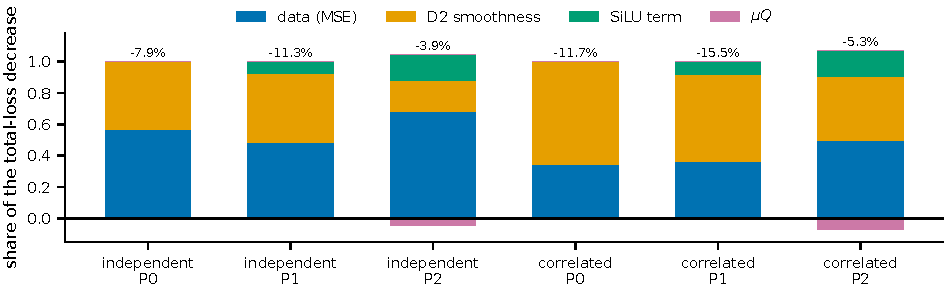
\includegraphics[width=\linewidth]{figS1_lossdecomp.pdf}
  % CAPTION-DRAFT: review (numbers from paper2/figures/figS1_lossdecomp.json)
  \caption{Post hoc loss decomposition (synthetic, early$\to$polished): share of the total-loss decrease from each term, pooled over the 8 seeds of each cell. independent P0: data 0.57, D2 0.43 (median total change -7.9\%); independent P1: data 0.49, D2 0.44 (median total change -11.3\%); independent P2: data 0.68, D2 0.20 (median total change -3.9\%); correlated P0: data 0.35, D2 0.65 (median total change -11.7\%); correlated P1: data 0.37, D2 0.55 (median total change -15.5\%); correlated P2: data 0.50, D2 0.40 (median total change -5.3\%).}
  \label{fig:S1}
\end{figure}


\begin{figure}[h]
  \centering
  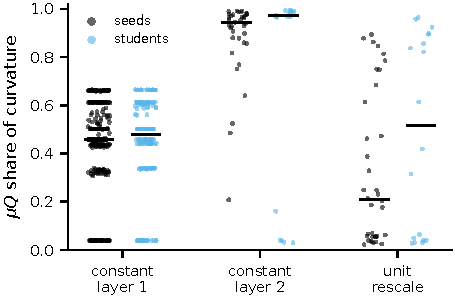
\includegraphics[width=0.5\linewidth]{figS2_gaugecheck.pdf}
  % CAPTION-DRAFT: review (numbers from paper2/figures/figS2_gaugecheck.json)
  \caption{Post hoc gauge check at the $\mu = 10^{-4}$ certified minima: share of the curvature along each least-squares gauge direction contributed by $\mu Q$. Medians: constant shift in layer 1, real-data seeds 0.46 ($n = 288$); constant shift in layer 1, students (trained on a frozen teacher) 0.48 ($n = 144$); constant shift in layer 2, real-data seeds 0.94 ($n = 36$); constant shift in layer 2, students 0.97 ($n = 18$); unit rescaling, real-data seeds 0.21 ($n = 36$); unit rescaling, students 0.52 ($n = 18$).}
  \label{fig:S2}
\end{figure}


\begin{figure}[h]
  \centering
  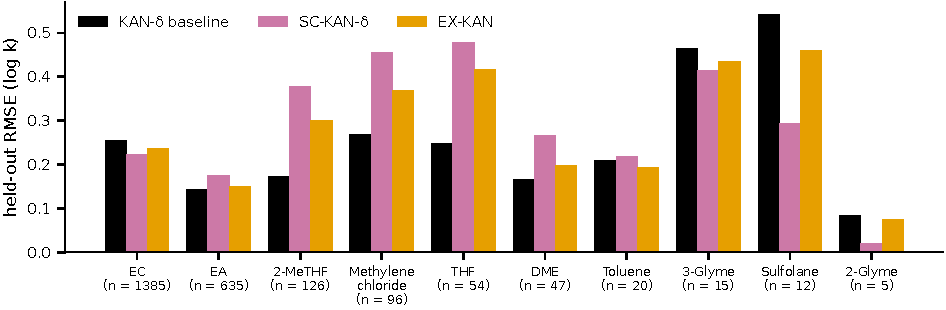
\includegraphics[width=\linewidth]{figS3_loco.pdf}
  % CAPTION-DRAFT: review (numbers from paper2/figures/figS3_loco.json)
  \caption{Leave-one-co-solvent-out RMSE per fold (5-seed ensembles, early state) for the KAN-$\delta$ baseline, SC-KAN-$\delta$ and EX-KAN. Unweighted means: KAN-$\delta$ baseline 0.2554; SC-KAN-$\delta$ 0.2923; EX-KAN 0.2834. The EA fold uses the fold A rows.}
  \label{fig:S3}
\end{figure}

\else % commit hashes replaced by neutral labels (commitmap.json is not part of the submission)
  % GENERATED by build_tex.py (anonymous: commit hashes replaced by labels, see commitmap.json)
\section{All pre-registered predictions}\label{app:prereg}

Generated by \texttt{F-01} from the committed verdict sections; the cell text is the committed wording. Commits are given as pre-registration $\to$ results (in the anonymous version, as neutral labels S-NN). Thresholds are part of each prediction's wording.

\subsection{Synthetic study (\texttt{F-02})}

{\footnotesize\setlength{\tabcolsep}{3pt}
\begin{longtable}{R{0.05\linewidth} R{0.29\linewidth} R{0.36\linewidth} R{0.09\linewidth} R{0.11\linewidth}}
\toprule
ID & Prediction (threshold) & Result & Verdict & Commits \\
\midrule
\endhead
X1 & runaway ($\geq$ 10) in correlated P0 and P1; $\leq$ 3 in the three independent cells and correlated P2 & Correlated P0 $\times$65.7 and P1 $\times$32.1, and P2 $\times$1.00, as predicted. \textbf{But independent P0 $\times$12.5 and P1 $\times$7.9 exceed 3} (independent P2 $\times$1.09) & \textbf{failed} & S-35$\to$\allowbreak S-36 \\
X2 & certified $\leq$ 2/8 in correlated P0 and P1; $\geq$ 6/8 elsewhere & correlated P0 0/8, P1 0/8; independent 6/8, 6/8, 8/8; correlated P2 8/8 & \textbf{held} & S-35$\to$\allowbreak S-36 \\
X3 & cancellation in correlated P0 and P1 each $\geq$ 2 $\times$ correlated P2 & P0 3.29 and P1 2.32, against 2 $\times$ 1.99 = 3.98 & \textbf{failed} & S-35$\to$\allowbreak S-36 \\
X4 & off-manifold ratio $\geq$ 3 in correlated P0 and P1, $\leq$ 1.5 in P2 & P0 1.22, P1 \textbf{0.77}; P2 0.78 (the P2 part held) & \textbf{failed} & S-35$\to$\allowbreak S-36 \\
X5 & Spearman(cancellation, off-manifold RMSE) $\geq$ 0.6 over the 24 correlated models & $\rho$ = +0.177, p = 0.407 & \textbf{failed} & S-35$\to$\allowbreak S-36 \\
X6 & unit match $\geq$ 0.85 in the independent cells and correlated P2; < 0.7 in correlated P0 and P1 & The first part held: 1.000 in all four no-runaway-predicted cells. \textbf{The second part failed: correlated P0 0.774 and P1 0.883 are not < 0.7} & \textbf{failed} & S-35$\to$\allowbreak S-36 \\
\bottomrule
\end{longtable}}
\subsection{Real-data case study (\texttt{F-03})}

Rows are as committed in the case-study summary (one row may cover several predictions, e.g.\ F2--F5). The rank intervention's verdicts are given per arm in the result column.

{\footnotesize\setlength{\tabcolsep}{3pt}
\begin{longtable}{R{0.14\linewidth} R{0.26\linewidth} R{0.29\linewidth} R{0.10\linewidth} R{0.11\linewidth}}
\toprule
Study & Prediction (threshold) & Result & Verdict & Commits \\
\midrule
\endhead
Gauge study (\texttt{gauge\_\allowbreak{}F-04}) & \textbf{Control 1}: teacher edges recovered, median dense corr $\geq$ 0.8 & 0.301 (sanity: h corr 0.913 < 0.95) & \textbf{failed} & S-02$\to$\allowbreak{}S-03 \\
Gauge study (\texttt{gauge\_\allowbreak{}F-04}) & P1: gauge fixing removes $\geq$ 50\% of edge variance & not run & inconclusive (gated by Control 1) & S-02$\to$\allowbreak{}S-03 \\
Gauge study (\texttt{gauge\_\allowbreak{}F-04}) & P2: sparse $\geq$ 2$\times$ dense, DEC region highest & not run & inconclusive (gated) & S-02$\to$\allowbreak{}S-03 \\
Gauge study (\texttt{gauge\_\allowbreak{}F-04}) & P3: (e) < (d) < (c) < (a) & not run & inconclusive (gated) & S-02$\to$\allowbreak{}S-03 \\
Gauge study (\texttt{gauge\_\allowbreak{}F-04}) & P4: every seed has a unit with |corr| < 0.8 & not run & inconclusive (gated) & S-02$\to$\allowbreak{}S-03 \\
Gauge study (\texttt{gauge\_\allowbreak{}F-04}) & P5: KAN-full edge variance > KAN-delta & not run & inconclusive (gated) & S-02$\to$\allowbreak{}S-03 \\
Gauge study (\texttt{gauge\_\allowbreak{}F-04}) & P6: seed spread flags errors & Spearman +0.169 (A) / +0.213 (B); fold B RMSE at 80\% coverage 0.153 vs random 0.137 & \textbf{failed} & S-02$\to$\allowbreak{}S-04 \\
Control 2 (\texttt{control2\_\allowbreak{}F-04}) & C1: (I,C) edges $\geq$ 0.9 and units $\geq$ 0.9 & prediction corr 0.947 < 0.99 & inconclusive (gate failed) & S-05$\to$\allowbreak{}S-06 \\
Control 2 (\texttt{control2\_\allowbreak{}F-04}) & C2: (R,C) invT, molal $\geq$ 0.9; co-solvent < 0.7 & prediction corr 0.969 < 0.99 & inconclusive (gate failed) & S-05$\to$\allowbreak{}S-06 \\
Control 2 (\texttt{control2\_\allowbreak{}F-04}) & C3: 107 epochs gives prediction corr < 0.95 & 0.858 (I,S), 0.919 (R,S) & \textbf{held} & S-05$\to$\allowbreak{}S-06 \\
Control 3 (\texttt{control3\_\allowbreak{}F-04}) & C1': (I) passes the gate, edges $\geq$ 0.9, units $\geq$ 0.9 & (I) RMSE/std 0.128 > 0.05; unit match 0.648 & \textbf{failed} & S-07$\to$\allowbreak{}S-08 \\
Control 3 (\texttt{control3\_\allowbreak{}F-04}) & C2': (R) edges $\leq$ (I) edges $-$ 0.10 & (R) edges 0.852, units 0.659 & inconclusive ((I) failed the gate) & S-07$\to$\allowbreak{}S-08 \\
Control 3 (\texttt{control3\_\allowbreak{}F-04}) & C4: every continuous input $\geq$ 0.9 in (I) & -- & inconclusive ((I) failed the gate) & S-07$\to$\allowbreak{}S-08 \\
Fiber (\texttt{fiber\_\allowbreak{}F-04}) & F1: $\geq$ 50\% of seed pairs on-fiber & 0/190 (closest d = 0.146) & \textbf{failed} & S-09$\to$\allowbreak{}S-10 \\
Fiber (\texttt{fiber\_\allowbreak{}F-04}) & F2--F5 & not run & inconclusive (no on-fiber pairs) & S-09$\to$\allowbreak{}S-10 \\
Fiber 2 (\texttt{fiber2\_\allowbreak{}F-04}) & G1: $\geq$ 4/6 seeds and $\geq$ 10/20 students certify convergence & 0/6, 0/20 (all at the 20,000-iteration cap) & \textbf{failed} & S-11$\to$\allowbreak{}S-12 \\
Fiber 2 (\texttt{fiber2\_\allowbreak{}F-04}) & G2--G5 & not run & inconclusive (no converged model) & S-11$\to$\allowbreak{}S-12 \\
Support (\texttt{support\_\allowbreak{}F-04}) & H1: dim(N) $\geq$ 5 & dim(N) = 36 of 72 & \textbf{held} & S-13$\to$\allowbreak{}S-14 \\
Support (\texttt{support\_\allowbreak{}F-04}) & H2: $\geq$ 50\% of N is REDISTRIBUTION within the correlated group & 18/36 & \textbf{held, exactly at threshold} & S-13$\to$\allowbreak{}S-14 \\
Support (\texttt{support\_\allowbreak{}F-04}) & H3: set A fraction in N $\geq$ 0.5 and $\geq$ 3$\times$ random & median 0.942 (random 0.5) & inconclusive (untestable: 3 $\times$ 0.5 > 1) & S-13$\to$\allowbreak{}S-14 \\
Support (\texttt{support\_\allowbreak{}F-04}) & H4: set B (capped), same criterion & median 0.949 & inconclusive (untestable) & S-13$\to$\allowbreak{}S-14 \\
Support (\texttt{support\_\allowbreak{}F-04}) & H5: flattest Hessian directions overlap N $\geq$ 0.5 & median 0.885; median layer-1 block share only 0.08 & \textbf{held}, with caveat (see \texttt{support\_\allowbreak{}F-04}) & S-13$\to$\allowbreak{}S-14 \\
Support (\texttt{support\_\allowbreak{}F-04}) & H6: fraction in N rises from control-3 to capped state, $\geq$ 15/20 & 20/20 (0.713 $\to$\allowbreak{} 0.949) & \textbf{held} & S-13$\to$\allowbreak{}S-14 \\
Rule (\texttt{rule\_\allowbreak{}F-04}) & I1--I5 (gate) & 0 columns removed; gate stopped & inconclusive & S-16$\to$\allowbreak S-17 \\
Rank (\texttt{rank\_\allowbreak{}F-04}) & I1: median max|grad| $\leq$ 0.1 $\times$ baseline & arm G: \textbf{failed} (4.00$\times$); arm F: \textbf{failed} (29.1$\times$) & see result & S-18$\to$\allowbreak S-19 \\
Rank (\texttt{rank\_\allowbreak{}F-04}) & I2: median d\_AB $\leq$ 0.5 $\times$ baseline & arm G: \textbf{failed} (0.945$\times$); arm F: \textbf{failed} (0.808$\times$) & see result & S-18$\to$\allowbreak S-19 \\
Rank (\texttt{rank\_\allowbreak{}F-04}) & I3 (sanity): median loss $\leq$ 1.10 $\times$ baseline & arm G: passed (1.004$\times$); arm F: passed, narrowly (1.099$\times$) & see result & S-18$\to$\allowbreak S-19 \\
Rank (\texttt{rank\_\allowbreak{}F-04}) & I4: fold A RMSE $\leq$ 0.150 (KAN-delta 0.1420) & arm G: \textbf{held}, narrowly (0.1499); arm F: \textbf{failed} (0.1587) & see result & S-18$\to$\allowbreak S-19 \\
Rank (\texttt{rank\_\allowbreak{}F-04}) & I5: edge corr on 1000/T and molality $\geq$ baseline + 0.1 (baseline 0.102) & arm G: \textbf{held} (0.927); arm F: \textbf{held} (0.338) & see result & S-18$\to$\allowbreak S-19 \\
Rank (\texttt{rank\_\allowbreak{}F-04}) & I6: arm F's improvement $\geq$ arm G's in both I1 and I2 & arm G: \textbf{failed} (max|grad| 29.1$\times$ vs 4.00$\times$; d\_AB does favour F, 0.808 vs 0.945) & see result & S-18$\to$\allowbreak S-19 \\
\texttt{trust\_\allowbreak{}F-04} & T1 / T2: trust-krylov certifies $\geq$ 4/6 seeds / $\geq$ 2/3 students & 0/6, 0/3. All 9 stopped on scipy's "bad approximation" after 1--62 iterations; the Hessian was accurate to $\leq$ 2e-7 & \textbf{failed} & S-20$\to$\allowbreak S-21 \\
\texttt{trust\_\allowbreak{}F-04} & T3--T5 & nothing converged & inconclusive & S-20$\to$\allowbreak S-21 \\
\texttt{stage2\_\allowbreak{}F-04} & U1: trust-exact (exact Hessian, 500 iterations) certifies $\geq$ 4/6 seeds & 0/6. All 9 hit the iteration cap & \textbf{failed} & S-22$\to$\allowbreak S-26 \\
\texttt{stage2\_\allowbreak{}F-04} & U2: with L2 $\lambda$ = 1e-5, $\geq$ 4/6 seeds and $\geq$ 2/3 students & 1/6 seeds, 0/3 students & \textbf{failed} & S-22$\to$\allowbreak S-26 \\
\texttt{stage2\_\allowbreak{}F-04} & U3: more converge at 1e-5 than at 1e-6 & 1 vs 0 & \textbf{held} & S-22$\to$\allowbreak S-26 \\
\texttt{stage2\_\allowbreak{}F-04} & U4: converged L2 models' loss without L2 $\leq$ 1.05 $\times$ capped & 1.2545 & \textbf{failed} & S-22$\to$\allowbreak S-26 \\
\texttt{stage2\_\allowbreak{}F-04} & U5: converged seeds' disagreement $\leq$ 0.5 $\times$ capped & only 1 converged & inconclusive & S-22$\to$\allowbreak S-26 \\
\texttt{close\_\allowbreak{}F-04} & V1: at some $\mu$, $\geq$ 4/6 seeds and $\geq$ 2/3 students converge (stage2 criterion) & 0 certified at every $\mu$ & \textbf{failed} & S-29$\to$\allowbreak{}S-30 \\
\texttt{close\_\allowbreak{}F-04} & V2: converged seeds' data term $\leq$ 1.05 $\times$ stage2 A & nothing certified at the selected $\mu$ = 1e-6 & inconclusive & S-29$\to$\allowbreak{}S-30 \\
\texttt{close\_\allowbreak{}F-04} & V3: $\|\theta\|^{2}$ $\leq$ 10 $\times$ start & same & inconclusive & S-29$\to$\allowbreak{}S-30 \\
\texttt{close\_\allowbreak{}F-04} & V4: seed disagreement halved & same & inconclusive & S-29$\to$\allowbreak{}S-30 \\
\texttt{close\_\allowbreak{}F-04} & V5: students' unit match $\geq$ 0.8 & same & inconclusive & S-29$\to$\allowbreak{}S-30 \\
\texttt{close\_\allowbreak{}F-04} & V6: fold A RMSE $\leq$ 0.150 & 1.0262, bias +0.9028 & \textbf{failed} & S-29$\to$\allowbreak{}S-30 \\
\texttt{certify\_\allowbreak{}F-04} & W1: at $\mu$ = 1e-4, $\geq$ 5/6 seeds certified (second-order criterion, F-a) & 6/6; all 17 candidates certified & \textbf{held} & S-31$\to$\allowbreak{}S-32 \\
\texttt{certify\_\allowbreak{}F-04} & W2: certified seeds' median d\_AB $\leq$ 0.5 $\times$ capped & 0.0771 vs capped 0.1041 ($-$26\%) & \textbf{failed} & S-31$\to$\allowbreak{}S-32 \\
\texttt{certify\_\allowbreak{}F-04} & W3: certified students' unit match $\geq$ 0.8 (vs the original teacher) & 0.624 & \textbf{failed} & S-31$\to$\allowbreak{}S-32 \\
\texttt{certify\_\allowbreak{}F-04} & W4: $\mu$ = 1e-4 fold A RMSE $\leq$ 0.150 & 0.3345 & \textbf{failed} & S-31$\to$\allowbreak{}S-32 \\
\texttt{certify\_\allowbreak{}F-04} & W5: $\mu$ = 1e-4 fold A RMSE $\leq$ 0.5131 & 0.3345 & \textbf{held} & S-31$\to$\allowbreak{}S-32 \\
\texttt{certify\_\allowbreak{}F-04} & W6: Spearman(cross-edge ratio, held-out RMSE) $\geq$ 0.6 & $\rho$ = +0.345, p = 0.328 (weak test) & \textbf{failed} & S-31$\to$\allowbreak{}S-32 \\
\bottomrule
\end{longtable}}
\noindent Committed tally of the case study:

{\footnotesize\setlength{\tabcolsep}{3pt}
\begin{longtable}{R{0.55\linewidth} r r r}
\toprule
Study & Held & Failed & Inconclusive \\
\midrule
\endhead
First table (Control 1, P1--P6, C1--C3, C1'/C2'/C4, F1--F5, G1--G5, H1--H6) & 5 & 5 & 19 \\
Rule (I1--I5) & 0 & 0 & 5 \\
Rank (I1, I2, I4, I5 per arm, I6) & 3 & 6 & 0 \\
Trust (T1--T5) & 0 & 2 & 3 \\
Stage 2 (U1--U5) & 1 & 3 & 1 \\
Close (V1--V6) & 0 & 2 & 4 \\
Certify (W1--W6) & 2 & 4 & 0 \\
\textbf{Total} & \textbf{11} & \textbf{22} & \textbf{32} \\
\bottomrule
\end{longtable}}
\subsection{Shared-curve KAN (\texttt{F-05})}

Run after the case-study close-out; not part of the 65 predictions above.

{\footnotesize\setlength{\tabcolsep}{3pt}
\begin{longtable}{R{0.05\linewidth} R{0.26\linewidth} R{0.39\linewidth} R{0.09\linewidth} R{0.11\linewidth}}
\toprule
ID & Prediction (threshold) & Result & Verdict & Commits \\
\midrule
\endhead
S1 & SC LOCO RMSE $\leq$ 1.05 $\times$ baseline & unweighted mean SC 0.2923 vs base 0.2554 (ratio 1.145; threshold 0.2681). Also reported: row-weighted 0.2478 / 0.2297 (1.079); folds $\geq$ 20 rows 0.3138 / 0.2093 (1.499) & failed & S-38$\to$\allowbreak S-40 \\
S2 & SC fold A RMSE $\leq$ 0.160 & SC 0.1757 (base 0.1420) & failed & S-38$\to$\allowbreak S-40 \\
S3 & SC median d\_AB $\leq$ 0.5 $\times$ baseline & SC 0.1865 vs base 0.1120 (threshold 0.0560): SC seeds agree \emph{less} than baseline seeds & failed & S-38$\to$\allowbreak S-40 \\
S4 & curve corr $\geq$ 0.90 for $\geq$ 6 of 8 inputs & 3 of 8 (M\_co 0.959, mix\_lneta 0.970, invT 0.986); lowest x\_co 0.596; others 0.871--0.891 & failed & S-38$\to$\allowbreak S-40 \\
S5 & $\geq$ 8/10 SC fold A models certified & SC 10/10 (max|grad| $\leq$ 7e-10, 0 near-null eigenvalues); baseline 0/10 (all hit the 500-iteration cap) & held & S-38$\to$\allowbreak S-40 \\
S6 & median $\beta$-norm polished/early $\leq$ 3 (calibrated) & median 1.337 (range 0.652--2.356); $\|\theta\|^{2}$ $\times$4.59 (base $\times$67.9, range 30.6--281) & held & S-38$\to$\allowbreak S-40 \\
S7 & SC polished/early fold A RMSE $\leq$ 1.5 & SC 1.920 (0.1757 $\to$\allowbreak{} 0.3373); baseline 5.736 (0.1420 $\to$\allowbreak{} 0.8147) & failed & S-38$\to$\allowbreak S-40 \\
S8 & d log k/d(1000/T) < 0 on $\geq$ 95\% rows in $\geq$ 8/10 seeds & 10/10 (median share 1.000; 1424 rows, 10 excluded per D4) & held & S-38$\to$\allowbreak S-40 \\
S9 & Spearman(1000/T, |slope|) > 0 in $\geq$ 8/10 seeds & 10/10 (median +0.661, range +0.406 to +0.885) & held & S-38$\to$\allowbreak S-40 \\
S10 & d log k/d(ln $\eta$\_mix) < 0 on $\geq$ 90\% rows in $\geq$ 8/10 seeds & 7/10 (median share 0.967; s0 0.892, s2 0.892, s8 0.826) & failed & S-38$\to$\allowbreak S-40 \\
\bottomrule
\end{longtable}}
\subsection{Two-anchor excess model (\texttt{F-06})}

Run after the case-study close-out; not part of the 65 predictions above.

{\footnotesize\setlength{\tabcolsep}{3pt}
\begin{longtable}{R{0.05\linewidth} R{0.26\linewidth} R{0.39\linewidth} R{0.09\linewidth} R{0.11\linewidth}}
\toprule
ID & Prediction (threshold) & Result & Verdict & Commits \\
\midrule
\endhead
E1 & EX LOCO $\leq$ 0.95 $\times$ KAN-delta & unweighted mean EX 0.2834 vs threshold 0.2426 (base 0.2554; ratio 1.110). Row-weighted 0.2363 / 0.2297 (1.029); folds $\geq$ 20 rows 0.2662 / 0.2093 (1.272). EX is better on EC (0.237 vs 0.256), Sulfolane, 3-Glyme, 2-Glyme and Toluene, and worse on 2-MeTHF, THF, Methylene chloride, DME and EA & failed & S-41$\to$\allowbreak S-43 \\
E2 & EX fold A $\leq$ 0.142 & EX 0.1502 (base this run 0.1420) & failed & S-41$\to$\allowbreak S-43 \\
E3 & s agrees across seeds (separable co-solvents, Amendment 1) & median pairwise corr +0.987 over EA, EC, Methylene chloride: a weak test with 3 values per seed, and Methylene chloride is marginal. Seed SD of s: EA 0.063 (0.39 $\times$ the spread across co-solvents, 0.159), EC 0.091 (0.57 $\times$), Methylene chloride 0.067 (0.42 $\times$). Secondary ($\leq$ 2 rule, 7 co-solvents): +0.869 & held & S-41$\to$\allowbreak S-43 \\
E4 & mean s(low $\varepsilon$) < mean s(EC, Sulfolane) in $\geq$ 8/10 seeds & 0/10: the ordering is reversed in every seed. Per high-$\varepsilon$ co-solvent: vs EC alone 0/10 (EC median s +0.104), vs Sulfolane alone 0/10 (median $-$0.124). The low-$\varepsilon$ mean is +0.19 to +0.49 per seed. Sulfolane does not drive the failure on its own: EC alone fails in every seed too & failed & S-41$\to$\allowbreak S-43 \\
E5 & median seed-SD flagged $\geq$ 2 $\times$ separable (Amendment 1) & 0.091 vs 0.067, ratio 1.37. Secondary ($\leq$ 2 rule): 0.222 vs 0.069, ratio 3.22, no verdict; the secondary is driven by 3-Glyme (SD 0.478, M\_co extrapolated) and 2-Glyme (0.222) & failed & S-41$\to$\allowbreak S-43 \\
\bottomrule
\end{longtable}}% GENERATED by build_tex.py (anonymous: commit hashes replaced by labels, see commitmap.json)
\section{Post-hoc analyses}\label{app:posthoc}

Every analysis below was defined after seeing results. Each is labelled \textbf{post hoc} in its own files, changes no pre-registered verdict, and is reported as exploratory. The description is the subject line of the commit that added the analysis.

{\footnotesize\setlength{\tabcolsep}{3pt}\begin{longtable}{R{0.28\linewidth} R{0.52\linewidth} R{0.10\linewidth}}
\toprule
Analysis & Commit subject (as committed) & Commit \\
\midrule
\endhead
\textbf{Post hoc.} Anatomy of the real-data runaway \newline \footnotesize{\texttt{F-07, F-08, F-09}} & Plan for descriptive runaway anatomy (before F-08 exists) & S-27 \\
 & Anatomy (descriptive): Q1, Q2 not as expected, Q3 as expected; RBF growth is in the penalty null space & S-28 \\
\textbf{Post hoc.} Gauge check and regularised teacher (exploratory) \newline \footnotesize{\texttt{F-10, F-11, F-12}} & gaugecheck (POST-HOC, exploratory): penalty fixes gauge position by slope balance; students match the regularised teacher & S-33 \\
\textbf{Post hoc.} Anatomy of the synthetic runaway \newline \footnotesize{\texttt{F-13, F-14}} & paper2 anatomy\_synth (POST-HOC, descriptive): synthetic runaway lives mainly in layer-2 output-edge cancellation, unsaturated; no verdicts change & S-37 \\
\textbf{Post hoc.} Loss decomposition along the runaway \newline \footnotesize{\texttt{F-15, F-16}} & paper2 lossdecomp (POST-HOC, descriptive): synthetic runaway loss decrease shared, D2 penalty median 0.61 vs data 0.37; 12/20 runaway models overfit; real-data reference recomputed & S-44 \\
\textbf{Post hoc.} Descriptive checks (hidden-unit correlation, tilt affinity, references) \newline \footnotesize{\texttt{F-17, F-18, F-19}} & paper2/checks: plan for descriptive checks (F4 hidden-unit correlation, F2 tilt affinity, A1 commit and data citation) before F-20 exists & S-46 \\
 & paper2/checks (POST-HOC, descriptive): hidden-unit correlation marks the runaway (independent cells 0.70 vs 0.05) but is not sufficient; RBF tilt affine to 2\% centrally, 13\% at the ends; A1 commit S-01; CALiSol-23 citation not in competition material & S-47 \\
\textbf{Post hoc.} Regularised teacher (weights pinned) & Pin gaugecheck regularised-teacher weights in a seventh archive; append to weights manifest & S-34 \\
\bottomrule
\end{longtable}}% GENERATED by build_tex.py (anonymous: commit hashes replaced by labels, see commitmap.json)
\section{Reproducibility map}\label{app:repro}

Generated from \texttt{F-42}. Every figure is rebuilt by its script from committed results; each figure's sidecar JSON lists the data files (path, commit, SHA-256), any archived weights (SHA-256, archive) and every plotted number. \REPOSTATEMENT

{\footnotesize\setlength{\tabcolsep}{3pt}
\begin{longtable}{R{0.15\linewidth} R{0.13\linewidth} R{0.42\linewidth} R{0.19\linewidth}}
\toprule
Figure & Script & Data files (commit) & Archived weights \\
\midrule
\endhead
Figure~\ref{fig:mechanism} \figname{fig1\_mechanism} & \texttt{F-43} & none (computed from committed code: F-02, F-44) & --- \\
Figure~\ref{fig:synthetic} \figname{fig2\_synthetic} & \texttt{F-45} & \texttt{F-46} (S-36) & --- \\
Figure~\ref{fig:where} \figname{fig3\_where} & \texttt{F-47} & \texttt{F-48} (S-88); \texttt{F-49} (S-37); \texttt{F-50} (S-48) & 18 files, archives W-01, W-02, W-03 \\
Figure~\ref{fig:applicability} \figname{fig4\_applicability} & \texttt{F-51} & \texttt{F-34} (S-90); \texttt{F-48} (S-88) & 15 files, archives W-04, W-05, W-06 \\
Figure~\ref{fig:paths} \figname{fig5\_paths} & \texttt{F-52} & \texttt{F-53} (S-59) & --- \\
Figure~\ref{fig:corrdose} \figname{fig6\_correlation\_dose} & \texttt{F-54} & \texttt{F-55} (S-64) & --- \\
Figure~\ref{fig:bspline} \figname{fig7\_bspline} & \texttt{F-56} & \texttt{F-46} (S-36); \texttt{F-57} (S-81); \texttt{F-30} (S-86) & --- \\
Figure~\ref{fig:dose} \figname{fig8\_dose\_response} & \texttt{F-58} & \texttt{F-59} (S-26); \texttt{F-60} (S-30); \texttt{F-61} (S-32) & --- \\
Figure~\ref{fig:uniqueness} \figname{fig9\_uniqueness} & \texttt{F-62} & \texttt{F-63} (S-41); \texttt{F-61} (S-32); \texttt{F-48} (S-88) & 40 files, archives W-05 \\
Figure~\ref{fig:S1} \figname{figS1\_lossdecomp} & \texttt{F-64} & \texttt{F-65} (S-46) & --- \\
Figure~\ref{fig:S2} \figname{figS2\_gaugecheck} & \texttt{F-64} & \texttt{F-66} (S-33) & --- \\
Figure~\ref{fig:S3} \figname{figS3\_loco} & \texttt{F-64} & \texttt{F-63} (S-41); \texttt{F-67} (S-45) & --- \\
\bottomrule
\end{longtable}}
\noindent Tables in the main text (no script; values typed in the draft):

{\footnotesize\setlength{\tabcolsep}{3pt}
\begin{longtable}{R{0.14\linewidth} R{0.14\linewidth} R{0.45\linewidth} R{0.16\linewidth}}
\toprule
Table & Source & Data files & Commits \\
\midrule
\endhead
Table~\ref{tab:synthetic} & typed in the draft from & \texttt{F-46}, \texttt{F-68} & S-36 \\
Table~\ref{tab:dose} & typed in the draft from & \texttt{F-60}, \texttt{F-61}, \texttt{F-59} & S-30, S-32, S-26 \\
Table~\ref{tab:alternatives} & typed in the draft from & \texttt{F-63}, \texttt{F-67}, \texttt{F-69} & S-41, S-45, S-49 \\
\bottomrule
\end{longtable}}
\noindent Panels evaluated post hoc from archived weights (from \texttt{F-70}):

\begin{itemize}
  \item \textbf{fig3a, real data:} the split of the parameter change into affine and curved RBF parts per layer, for 107 epochs $\to$\allowbreak{} fiber2 capped $\to$\allowbreak{} stage2 Part A.
  \item \texttt{F-59} stores only per-block norms, without an affine/curved split and without the 107 $\to$\allowbreak{} capped change.
  \item \textbf{fig9b, polished fold A d\_AB} for SC-KAN-$\delta$ and the baseline (marked *).
  \item arch/sc committed d\_AB only at the early state.
  \item \textbf{fig4a, b, fold A per-row error change} (early-stopped -> mu = $10^{-6}$ and mu = $10^{-4}$ ensembles).
  \item F-71 stores only the per-row Spearman correlations and medians; the per-row values are re-evaluated with the
\end{itemize}% GENERATED by build_tex.py (anonymous: commit hashes replaced by labels, see commitmap.json)
\section{Research process}\label{app:process}

% DRAFT-TEXT: review (new prose, not in the source draft; it states only the protocol followed, no results). First and last paragraphs: author-supplied wording (2026-10-05)
\paragraph{Pre-registration.} Every study committed a pre-registration file (predictions, thresholds, interpretation rules) before the script that tested it existed. Verdicts were appended below the committed text; the pre-registered text was never edited, and corrections to reported numbers were made in separate, labelled commits.
\paragraph{Amendments.} A change to a design after its pre-registration was committed as a dated amendment section before any affected model was trained, with its reason; the original text was kept. Choices forced by the code or data at run time were logged as numbered discrepancies at the top of each output log.
\paragraph{Files win.} Instructions to the agent stated that committed files take precedence over any number or description in a prompt; discrepancies between a brief and the files were flagged rather than resolved silently.
\paragraph{Data and weights.} Model weights were never committed: they were archived outside the repository with a manifest of SHA-256 hashes and producing commits, and every later analysis verified the hashes and held its inputs in memory. Post-hoc analyses were labelled as such in their files and changed no verdict.
\paragraph{AI assistance.} Code, runs and logs were produced by an AI coding agent working under this protocol. Study designs, briefs and the manuscript were developed with an AI assistant. The author set the research questions, reviewed and approved every brief and amendment, decided each next stage, and takes responsibility for all content. Crashes were recorded in the logs and fixed in separate commits labelled as implementation-only.

\noindent Pre-registrations, amendments and crash records (from the commit history):

{\footnotesize\setlength{\tabcolsep}{3pt}
\begin{longtable}{R{0.08\linewidth} R{0.10\linewidth} R{0.14\linewidth} R{0.58\linewidth}}
\toprule
Commit & Date & Kind & Commit subject \\
\midrule
\endhead
S-02 & 2026-09-23 & pre-registration & Pre-register KAN identifiability study (before any experiment) \\
S-05 & 2026-09-23 & pre-registration & Pre-register corrected 2x2 control (before writing or running it) \\
S-07 & 2026-09-23 & pre-registration & Pre-register control 3: reachable teacher (before writing code) \\
S-09 & 2026-09-29 & pre-registration & Pre-register fiber completeness test (before writing or running F-41) \\
S-11 & 2026-09-29 & pre-registration & Pre-register fiber2: certified convergence + teacher-known fiber analysis (before writing code) \\
S-13 & 2026-09-29 & pre-registration & Pre-register support study: near-null space, where models differ, Hessian (before F-42 exists) \\
S-15 & 2026-09-29 & pre-registration & Close-out: electrolyte case study summary (all pre-registered predictions) \\
S-16 & 2026-09-29 & pre-registration & Pre-register basis-size rule intervention (before F-43 exists) \\
S-18 & 2026-09-29 & pre-registration & Pre-register rank-constrained layer-1 intervention (before F-44 exists) \\
S-20 & 2026-09-30 & pre-registration & Pre-register trust-region Newton polishing, stage 1 (before F-45 exists) \\
S-22 & 2026-09-30 & pre-registration & Pre-register stage 2: trust-exact check, runaway diagnostic, coercivity (before F-46 exists) \\
S-23 & 2026-09-30 & crash record / fix & F-46 as first run (crashed with AttributeError in callback) \\
S-24 & 2026-09-30 & crash record / fix & stage2: fix AttributeError (implementation only, post-prereg) \\
S-25 & 2026-10-02 & crash record / fix & stage2: hold verified inputs in memory (implementation only, post-prereg) \\
S-29 & 2026-10-02 & pre-registration & Pre-register targeted null-space penalty intervention (before F-47 exists) \\
S-31 & 2026-10-03 & pre-registration & Pre-register second-order certification and regularised fold A accuracy (before F-48 exists) \\
S-35 & 2026-10-03 & pre-registration & paper2: pre-register synthetic 2x3 runaway test (before F-49 exists) \\
S-38 & 2026-10-03 & pre-registration & arch: pre-register SC-KAN-$\delta$ (shared-curve KAN-$\delta$) before any script exists; decisions C (centring), mu null-space term, tanh salt embedding, full beta term \\
S-39 & 2026-10-03 & crash record / fix & arch sc\_run: fix log() call (crash record 1, after the first fold A polish); resume from cache \\
S-41 & 2026-10-04 & pre-registration & arch: pre-register EX-KAN (two-anchor excess model) before any script exists; decision B (x\_co-independent g, [7,6,1]), full set for E3-E5, E4 mean rule \\
S-42 & 2026-10-04 & amendment & arch ex\_prereg: Amendment 1 (after Step 0, before training): primary separability rule by fixed-composition groups (EA, EC, Methylene chloride separable); committed rule reported as secondary \\
\bottomrule
\end{longtable}}% GENERATED by build_tex.py (anonymous: commit hashes replaced by labels, see commitmap.json)
\section{Supplementary figures}\label{app:supp}


\begin{figure}[htbp]
  \centering
  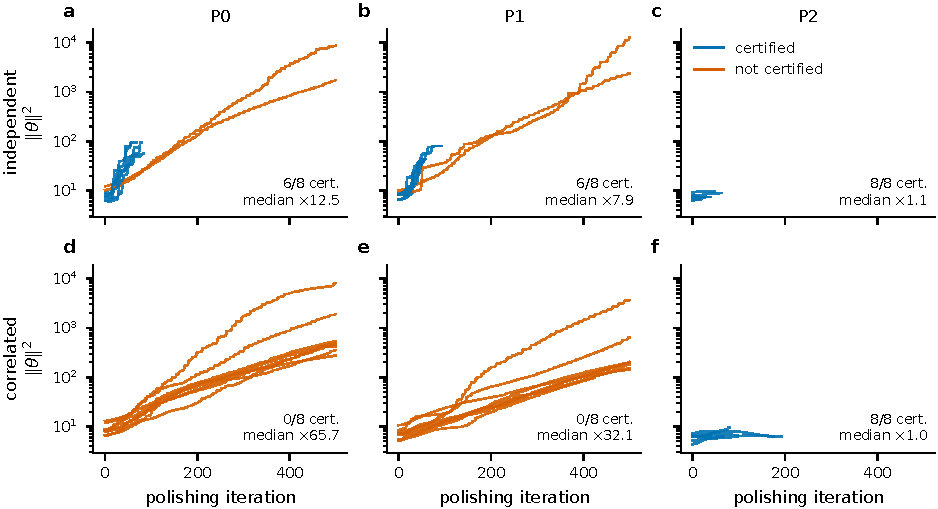
\includegraphics[width=\linewidth]{fig2_synthetic.pdf}
  % CAPTION-DRAFT: review (numbers from paper2/figures/fig2_synthetic.json)
  \caption{Synthetic $2\times3$ study: $\|\theta\|^2$ over exact-Hessian trust-region polishing iterations (log scale), one line per seed, coloured certified (blue) or not certified (vermillion). Rows: independent and correlated inputs; columns: P0, P1, P2. Per panel, certified seeds and median growth (polished over early-stopped): independent P0: 6/8 certified, $\times$12.5; independent P1: 6/8 certified, $\times$7.9; independent P2: 8/8 certified, $\times$1.1; correlated P0: 0/8 certified, $\times$65.7; correlated P1: 0/8 certified, $\times$32.1; correlated P2: 8/8 certified, $\times$1.0.}
  \label{fig:synthetic}
\end{figure}


\begin{figure}[htbp]
  \centering
  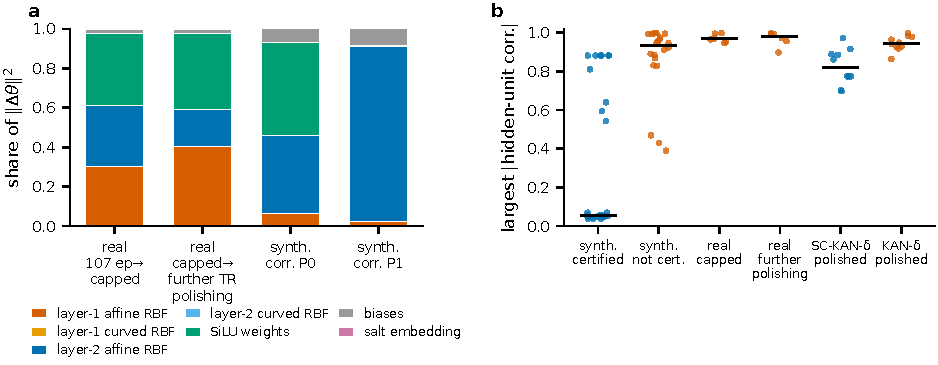
\includegraphics[width=\linewidth]{fig3_where.pdf}
  % CAPTION-DRAFT: review (numbers from paper2/figures/fig3_where.json)
  \caption{Where the runaway lives. \textbf{(a)} Mean share of $\|\Delta\theta\|^2$ by parameter block. Real data, 107 epochs$\to$capped: layer-1 affine RBF 0.30, layer-2 affine RBF 0.31, SiLU weights 0.37; capped$\to$further trust-region polishing: 0.40, 0.19, 0.38; synthetic correlated P0: layer-2 affine RBF 0.39, SiLU weights 0.47; correlated P1: layer-2 affine RBF 0.89. The real-data split was evaluated post hoc from archived weights (Appendix~\ref{app:repro}). \textbf{(b)} Largest absolute correlation between hidden-unit activations on the training rows, median: synthetic, certified 0.054 ($n=28$); synthetic, not certified 0.935 ($n=20$); real, capped 0.968 ($n=6$); real, further polishing 0.983 ($n=6$); SC-KAN-$\delta$ polished 0.818 ($n=10$); KAN-$\delta$ polished 0.946 ($n=10$). Blue: certified; vermillion: not certified or runaway.}
  \label{fig:where}
\end{figure}


\begin{figure}[htbp]
  \centering
  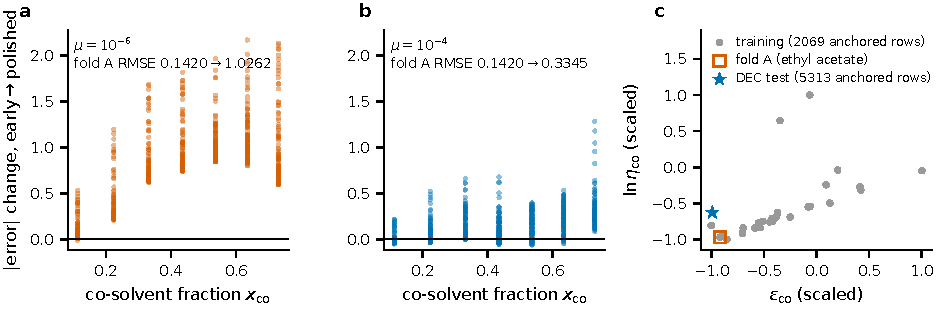
\includegraphics[width=\linewidth]{fig4_applicability.pdf}
  % CAPTION-DRAFT: review (numbers from paper2/figures/fig4_applicability.json)
  \caption{Applicability (descriptive; analysis plan committed before computing). \textbf{(a, b)} Fold A (ethyl acetate held out, 635 rows): change in each row's absolute error from the early-stopped 5-seed ensemble to the polished ensemble, against the co-solvent fraction $x_{\mathrm{co}}$ (7 distinct values); fold A RMSE 0.1420$\to$1.0262 at $\mu = 10^{-6}$ (a) and 0.1420$\to$0.3345 at $\mu = 10^{-4}$ (b). Per-row values are evaluated post hoc from SHA-verified archived weights, with the logged RMSEs reproduced (Appendix~\ref{app:repro}). \textbf{(c)} Co-solvent descriptors $\varepsilon_{\mathrm{co}}$ and $\ln\eta_{\mathrm{co}}$ in the committed min--max scaling: the 2069 anchored training rows (30 distinct points), fold A's co-solvent (off-pattern distance 0.047) and the 5313 anchored DEC test rows (0.334); each held-out set occupies a single point.}
  \label{fig:applicability}
\end{figure}


\begin{figure}[htbp]
  \centering
  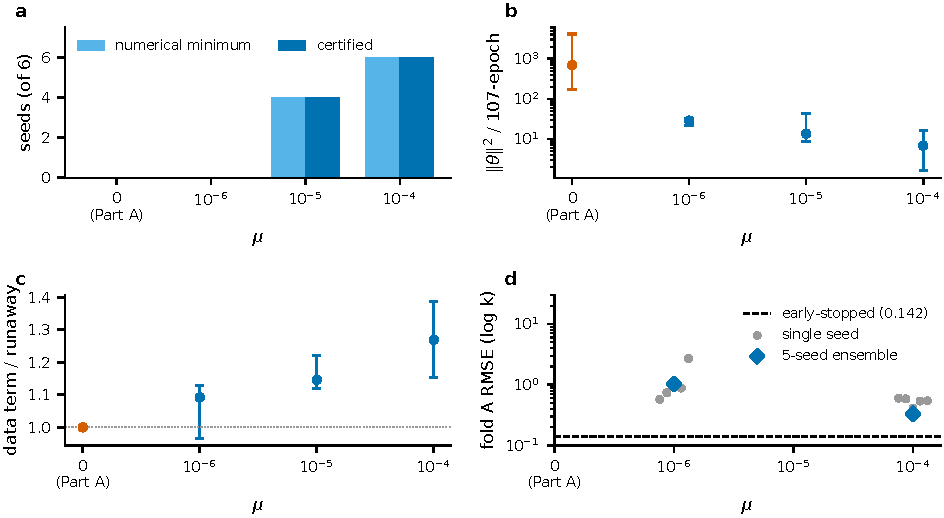
\includegraphics[width=\linewidth]{fig8_dose_response.pdf}
  % CAPTION-DRAFT: review (numbers from paper2/figures/fig8_dose_response.json)
  \caption{Real-data dose-response in the null-space weight $\mu$ (6 KAN-$\delta$ seeds; $\mu = 0$: polished without a null-space penalty). \textbf{(a)} Seeds at a numerical minimum (all of them certified): $\mu = 0$, 0 of 6; $10^{-6}$, 0 of 6; $10^{-5}$, 4 of 6; $10^{-4}$, 6 of 6. \textbf{(b)} $\|\theta\|^2$ relative to the 107-epoch state, median (range): $\mu = 0$, 690 (170--4146); $10^{-6}$, 29 (21--31); $10^{-5}$, 14 (9--43); $10^{-4}$, 7 (2--16). \textbf{(c)} Training data term relative to the runaway, median: $10^{-6}$, 1.092; $10^{-5}$, 1.146; $10^{-4}$, 1.269. \textbf{(d)} Fold A RMSE: early-stopped 0.142 (dashed line); polished 5-seed ensemble 1.026 at $\mu = 10^{-6}$ and 0.334 at $\mu = 10^{-4}$; grey points are single seeds.}
  \label{fig:dose}
\end{figure}


\begin{figure}[h]
  \centering
  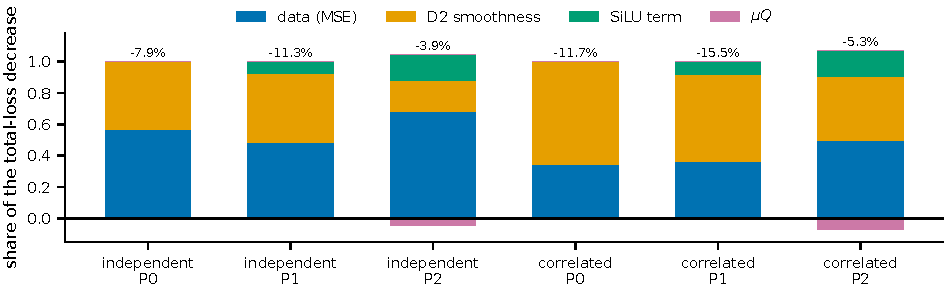
\includegraphics[width=\linewidth]{figS1_lossdecomp.pdf}
  % CAPTION-DRAFT: review (numbers from paper2/figures/figS1_lossdecomp.json)
  \caption{Post hoc loss decomposition (synthetic, early$\to$polished): share of the total-loss decrease from each term, pooled over the 8 seeds of each cell. independent P0: data 0.57, D2 0.43 (median total change -7.9\%); independent P1: data 0.49, D2 0.44 (median total change -11.3\%); independent P2: data 0.68, D2 0.20 (median total change -3.9\%); correlated P0: data 0.35, D2 0.65 (median total change -11.7\%); correlated P1: data 0.37, D2 0.55 (median total change -15.5\%); correlated P2: data 0.50, D2 0.40 (median total change -5.3\%).}
  \label{fig:S1}
\end{figure}


\begin{figure}[h]
  \centering
  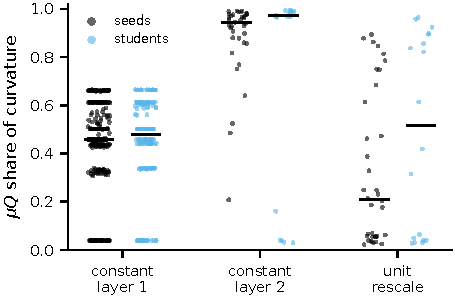
\includegraphics[width=0.5\linewidth]{figS2_gaugecheck.pdf}
  % CAPTION-DRAFT: review (numbers from paper2/figures/figS2_gaugecheck.json)
  \caption{Post hoc gauge check at the $\mu = 10^{-4}$ certified minima: share of the curvature along each least-squares gauge direction contributed by $\mu Q$. Medians: constant shift in layer 1, real-data seeds 0.46 ($n = 288$); constant shift in layer 1, students (trained on a frozen teacher) 0.48 ($n = 144$); constant shift in layer 2, real-data seeds 0.94 ($n = 36$); constant shift in layer 2, students 0.97 ($n = 18$); unit rescaling, real-data seeds 0.21 ($n = 36$); unit rescaling, students 0.52 ($n = 18$).}
  \label{fig:S2}
\end{figure}


\begin{figure}[h]
  \centering
  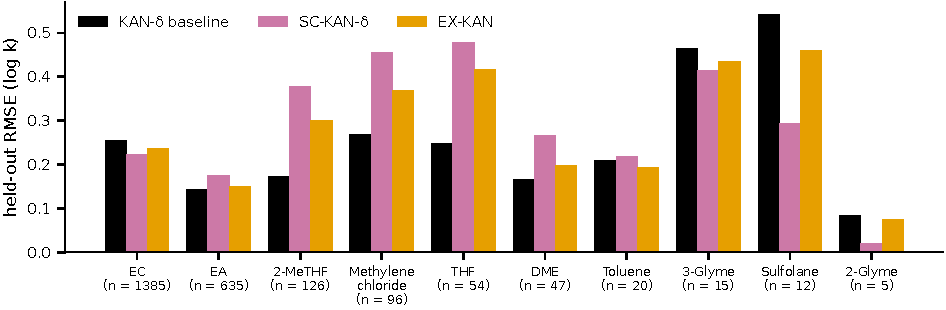
\includegraphics[width=\linewidth]{figS3_loco.pdf}
  % CAPTION-DRAFT: review (numbers from paper2/figures/figS3_loco.json)
  \caption{Leave-one-co-solvent-out RMSE per fold (5-seed ensembles, early state) for the KAN-$\delta$ baseline, SC-KAN-$\delta$ and EX-KAN. Unweighted means: KAN-$\delta$ baseline 0.2554; SC-KAN-$\delta$ 0.2923; EX-KAN 0.2834. The EA fold uses the fold A rows.}
  \label{fig:S3}
\end{figure}

\clearpage  % flush Appendix E's figures before Appendix F
\fi

\end{document}
.
% Generated parts (do not edit by hand; run build_tex.py): title.tex, body.tex, appendixA-E.tex.
\documentclass[10pt]{article}
\ifdefined\PREPRINT
  \usepackage[preprint]{tmlr}
\else
  \usepackage{tmlr}
\fi
\usepackage[utf8]{inputenc}
\usepackage{amsmath,amssymb}
\usepackage{graphicx}
\usepackage{booktabs}
\usepackage{longtable}
\usepackage{array}
\usepackage{url}
\usepackage[hidelinks]{hyperref}
\graphicspath{{../figures/}}
\newcolumntype{R}[1]{>{\raggedright\arraybackslash}p{#1}}

\title{Runaway edges: a smoothness-penalty blind spot makes Kolmogorov--Arnold networks non-identifiable on correlated inputs}


\ifdefined\PREPRINT
  \author{\name Gelavizh Ahmadi \\
          \addr Independent researcher, Berlin, Germany \\
          \addr ORCID: 0000-0000-0000-0000 % ORCID-PLACEHOLDER: replace before posting
          }
  \newcommand{\figname}[1]{(\texttt{#1})}
  \newcommand{\REPOSTATEMENT}{Code, committed results and figure scripts: \url{https://github.com/drgelavizhahmadi-dotcom/battery_hacketon}.}
  \hypersetup{pdftitle={Runaway edges: a smoothness-penalty blind spot makes Kolmogorov-Arnold networks non-identifiable on correlated inputs},
              pdfauthor={Gelavizh Ahmadi}}
\else
  % anonymous build: no author, affiliation, acknowledgments or repository URL anywhere in the source that reaches the PDF
  \author{}
  \newcommand{\figname}[1]{}
  \newcommand{\REPOSTATEMENT}{Code will be released upon publication.}
  \hypersetup{pdftitle={Runaway edges: a smoothness-penalty blind spot makes Kolmogorov-Arnold networks non-identifiable on correlated inputs},
              pdfauthor={}, pdfsubject={}, pdfkeywords={}, pdfcreator={LaTeX}}
\fi

\begin{document}
\maketitle

% GENERATED by build_tex.py from paper2/draft/paper2_draft.md -- do not edit by hand
\begin{abstract}
Kolmogorov--Arnold networks (KANs) are promoted as interpretable because each edge carries a learned univariate function. We show that a widely used family of smoothness penalties leaves a blind spot that undermines this promise: second-difference and curvature penalties do not charge for affine components of an edge, and SiLU base weights are often unpenalised. When the inputs to a layer are correlated, affine components on different edges can cancel inside a unit, so training inflates the parameters along directions that neither the penalty nor the data can see; the loss has no reachable finite minimum and independent runs never agree. In a pre-registered synthetic study with a known teacher, correlated inputs gave 0 of 16 converged models (median squared-norm growth 32--66$\times$), including under a recently proposed curvature penalty that also penalises the SiLU weight, while a small penalty on the affine null space gave 16 of 16 certified minima and exact recovery of the teacher's internals. On real electrolyte-conductivity data the same mechanism explains why no model converged, and polishing beyond early stopping under a weak null-space penalty degraded held-out accuracy (RMSE 0.142 $\to$\allowbreak{} 1.03). Closing the blind spot restores certified minima but leaves several distinct minima, so convergence and identifiability are separate problems. We give practical recommendations for penalised KANs.

\end{abstract}

\section{Introduction}\label{sec:1}

KANs replace a network's fixed activations with learned univariate functions on every edge. Their appeal for science rests on reading those functions: an edge that looks like an exponential decay suggests a physical law. That reading presumes the edges are determined by the data. If different training runs produce different edges with equally good predictions, the edges describe the optimiser, not the system.

This paper identifies a concrete, common mechanism that breaks that presumption. It arises from the interaction of three ingredients that are each standard in practice:

\begin{enumerate}
  \item \textbf{A smoothness penalty with an affine null space.} Second-difference (P-spline) penalties and curvature penalties ignore straight-line components of an edge; SiLU base terms are frequently unpenalised.
  \item \textbf{Correlated inputs to a layer.} Physical descriptors often move together. Hidden units can also become correlated during training, exposing the next layer.
  \item \textbf{Training toward convergence.} Early stopping hides the problem; longer optimisation exposes it.
\end{enumerate}

Together they create directions along which edges grow into large, mutually cancelling affine shapes. The penalty does not see them, and on the training data their contributions cancel. The loss keeps decreasing slightly along these directions, so it has no reachable finite minimum. Seeds wander apart, no model certifies as converged, and on inputs off the training correlation pattern the cancellation fails.

\textbf{Contributions.}

\begin{itemize}
  \item We describe the mechanism and show that it applies to any layer whose inputs are correlated, including the output layer (Section 3).
  \item In a pre-registered synthetic study, we show causally that a recently proposed curvature penalty does not prevent the runaway on correlated inputs, while a small additional penalty on the affine null space prevents it and restores exact recovery of a known solution (Section 4).
  \item On real electrolyte-conductivity data, we trace a complete failure to converge to this mechanism and document its effect on extrapolation (Section 5).
  \item We show that closing the blind spot yields certified, isolated minima but not uniqueness, and that structured alternatives trade accuracy for stability (Section 6).
  \item We give recommendations for penalised KANs (Section 7).
\end{itemize}

All experiments were pre-registered: predictions, thresholds and interpretation rules were committed before the code that tested them. Of 65 predictions in the real-data case study, 11 held, 22 failed and 32 were inconclusive; we report them as recorded.

\section{Background and related work}\label{sec:2}

\textbf{KAN edges.} A KAN layer maps inputs to outputs by summing learned univariate functions, one per edge. In the original formulation \citep{liu2025kan} each edge is a SiLU base term plus a B-spline expansion. FastKAN \citep{li2024fastkan} approximates the B-splines with Gaussian radial basis functions on fixed centres, which is the edge type used in our experiments:

\begin{equation}
  \varphi(x) = \alpha\,\mathrm{SiLU}(x) + \sum_{k=1}^{K} c_k \exp\!\left(-\left(\frac{x-\mu_k}{h}\right)^{2}\right)
\end{equation}

\textbf{Smoothness penalties and their null spaces.} P-spline penalties charge squared second differences of the coefficients \citep{eilers1996psplines}. Constant and linear coefficient patterns cost nothing: the penalty's null space is affine. In generalised additive models this is well understood, and \citet{marra2011double} proposed an additional penalty on the null space (the "double penalty") for variable selection. Our fix is the same construction; what is new is its consequence inside a KAN, where edges are summed within units and passed through further layers.

\textbf{Curvature penalties for KANs.} \citet{bagrow2026curvature} proposed per-edge curvature penalties for compositional smoothness, combining the second-difference penalty with a term $K_{\mathrm{silu}}\,\alpha^{2}$ on the SiLU weight, and noted that the penalty has affine functions as its null space by design. That work evaluated on independent, uniformly sampled inputs. Second-derivative penalties on spline coefficients also appear in other KAN variants, typically on the spline part only, leaving the SiLU base term free (\citealp{cang2024kanwork}; see also the free-knots KAN of \citealp{zheng2025freeknots}). We show that the affine null space becomes a runaway direction when inputs are correlated, and that penalising the SiLU weight alone does not close it.

\textbf{Concurvity.} In additive models, correlated inputs let one input's shape function absorb another's, making shape functions non-identifiable; this is known as concurvity. \citet{siems2023concurvity} proposed a regulariser penalising correlations between transformed features. The cross-edge cancellation we describe is concurvity inside a KAN unit. In an additive model with a penalised null space it shifts shape between functions; combined with an unpenalised affine null space in a KAN, it becomes unbounded growth.

\textbf{Losses without a finite minimum.} When a loss attains its infimum only at infinity, gradient descent drives the parameter norm to diverge, slowly, and optimisation can continue while held-out performance worsens \citep{soudry2018implicit}. Our runaway is an instance of this behaviour created by a penalty's null space.

\textbf{Parameter-space symmetries.} Exact symmetries (unit permutations, sign flips) make parameters non-identifiable in tanh and RBF networks, and completeness results characterise them \citep{sussmann1992uniqueness,kurkova1994uniqueness}. KANs add continuous symmetries such as affine reparametrisations of hidden units. The runaway is not an exact symmetry: it is an approximate one, a nearly flat but tilted direction, which is what prevents convergence.

\section{Mechanism}\label{sec:3}

Consider a unit that sums edges from two inputs, $s = \varphi_1(x_1) + \varphi_2(x_2)$, each edge as in Section 2, trained with a second-difference penalty on its RBF coefficients.

\textbf{Step 1: a direction the penalty cannot see.} Add a linear pattern $t\,\ell$ to the RBF coefficients of edge 1 and subtract it from edge 2, with $\ell_k$ proportional to the centre index. Linear coefficient patterns have zero second difference, so the penalty is unchanged for every t (Figure~\ref{fig:mechanism}b). With Gaussian bumps on a regular grid, the pattern produces a nearly affine function: over the central 80\% of the input range it deviates from a straight line by at most 2\% of its range (Figure~\ref{fig:mechanism}a), and by up to 13\% near the grid edges. Edge 1 thus gains approximately $t\,a\,x_1$ and edge 2 loses $t\,a\,x_2$.

\textbf{Step 2: a direction the data cannot see.} The unit's pre-activation changes by approximately $t\,a\,(x_1 - x_2)$. If $x_{1}$ and $x_{2}$ are strongly correlated, $x_1 - x_2$ is small wherever the data lie, so predictions change little even for large t (Figure~\ref{fig:mechanism}c). The direction is nearly free in both the penalty and the data.


\begin{figure}[t]
  \centering
  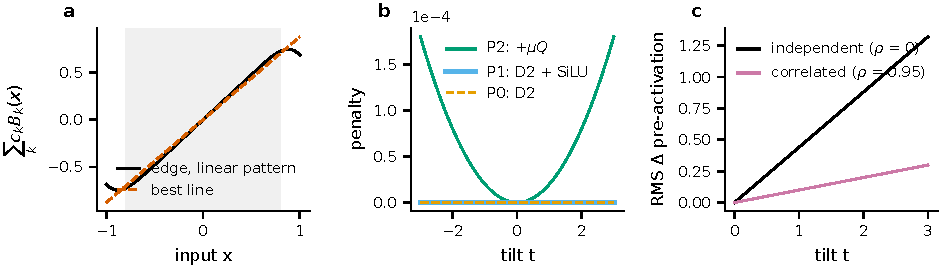
\includegraphics[width=\linewidth]{fig1_mechanism.pdf}
  % CAPTION-DRAFT: review (numbers from paper2/figures/fig1_mechanism.json)
  \caption{Mechanism (computed illustration) for the edge type of Section~\ref{sec:2} (8 Gaussian RBFs on $[-1, 1]$). \textbf{(a)} Edge function produced by a unit linear coefficient pattern and its best straight line; the shaded band is the central 80\% of the range, where the maximum deviation is 2.0\% of the function's range (12.9\% over the full range). \textbf{(b)} Penalty as a function of a tilt $t$ applied as $+t$ to edge 1 and $-t$ to edge 2: the second-difference penalty (P0) and P1 are exactly zero for every $t$; only P2's term $\mu Q$ grows ($\lambda = 0.001$, $\mu = 1e-05$). \textbf{(c)} RMS change in the unit's pre-activation per unit tilt: 0.0996 on correlated inputs ($\rho = 0.95$) against 0.4403 on independent inputs (4.42$\times$).}
  \label{fig:mechanism}
\end{figure}

\textbf{Step 3: no finite minimum.} "Nearly free" is not "free". Moving along it lets the model shed curvature into the free affine and SiLU components, so the loss decreases monotonically along the direction. Both terms contribute (post-hoc decomposition). In the synthetic runaway models the smoothness penalty fell to about a quarter of its early value and supplied a median 61\% of the decrease, while training error fell only 5\%. On real data, from early stopping to the capped state, the penalty fell 8--88$\times$ but supplied 17--36\% of the decrease, the data term the rest. In both, the growth went into whatever the penalty left free: the linear part of the RBF coefficients grew 34--40$\times$ in the synthetic runaway cells, and the SiLU weights 85$\times$ where they were unpenalised. In 12 of 20 synthetic runaway models, training error fell while test error rose. The infimum lies at infinity: gradients stay small but non-zero, the parameter norm grows without bound, and no minimum can be certified. Different seeds drift along different such directions.

\textbf{Step 4: any layer can be affected.} The argument needs only correlated inputs to a layer. Hidden units can become correlated during training, and then the output layer can host the same runaway even when the raw inputs are independent. Correlated hidden units appear necessary for this but not sufficient: they also occur in models that converge once the null space is penalised. Section 4 shows both forms.

\textbf{Consequences.}

\begin{itemize}
  \item \textbf{Non-identifiability:} edges differ across seeds by large affine components that leave predictions almost unchanged.
  \item \textbf{Non-convergence:} second-order optimisers stall; certification criteria fail.
  \item \textbf{Extrapolation risk:} off the training correlation pattern, $x_1 - x_2$ is no longer small, and the inflated components stop cancelling.
\end{itemize}

\textbf{The fix.} Penalise the null space directly. For each edge, let $P_{\mathrm{null}}$ project its RBF coefficients onto constant-plus-linear patterns in the centre index, and add

\begin{equation}
  Q = \sum_{e} \lVert P_{\mathrm{null}}\, c_e \rVert^{2}
\end{equation}

with a small weight $\mu$, in addition to a penalty on the SiLU weight. This makes every affine component cost something, which turns the infinite descent into a finite minimum.

\section{Controlled study}\label{sec:4}

\textbf{Design.} A teacher KAN [4, 3, 1] with smooth, hand-specified edges (fitted by smoothness-penalised least squares) generates targets with Gaussian noise of 5\% of the output spread; n = 2000 training rows. Inputs are $\mathcal{N}(0, 1)/3$, clipped to the grid, either independent or correlated in pairs ($\rho$ = 0.95 for $x_1/x_2$ and $x_3/x_4$). Students share the teacher's architecture and are trained under three penalty levels:

\begin{itemize}
  \item \textbf{P0:} second-difference penalty on RBF coefficients ($\lambda$ = $10^{-3}$).
  \item \textbf{P1:} P0 plus $K_{\mathrm{silu}}\,\alpha^{2}$ on each SiLU weight (Bagrow-style curvature penalty, $K_{\mathrm{silu}}$ = 0.443).
  \item \textbf{P2:} P1 plus $\mu Q$, the affine null-space penalty.
\end{itemize}

Each of the 6 cells has 8 seeds. Each student is trained with AdamW and early stopping, then polished with an exact-Hessian trust-region method and certified by a second-order criterion (gradient, curvature and Newton decrement). $\mu$ was calibrated before the experiment by a pre-registered rule: $10^{-6}$ failed the pilot (5.0$\times$ growth) and $10^{-5}$ passed (1.32$\times$) and was frozen.

\textbf{The teacher itself runs away.} Polished under P0 and P1 on correlated inputs, the teacher's parameters grew 85$\times$ and 1069$\times$ without certifying, while its predictions stayed within half a noise standard deviation of the original. The runaway changes the parameters, not the function.

\begin{table}[t]
  \centering
  % CAPTION-DRAFT: review
  \caption{Synthetic $2\times3$ study, per cell.}
  \label{tab:synthetic}
  \small
  \begin{tabular}{lp{0.2\linewidth}p{0.2\linewidth}p{0.2\linewidth}p{0.2\linewidth}p{0.2\linewidth}p{0.2\linewidth}p{0.2\linewidth}p{0.2\linewidth}p{0.2\linewidth}p{0.2\linewidth}p{0.2\linewidth}p{0.2\linewidth}p{0.2\linewidth}p{0.2\linewidth}p{0.2\linewidth}p{0.2\linewidth}p{0.2\linewidth}p{0.2\linewidth}p{0.2\linewidth}p{0.2\linewidth}p{0.2\linewidth}p{0.2\linewidth}p{0.2\linewidth}p{0.2\linewidth}p{0.2\linewidth}p{0.2\linewidth}p{0.2\linewidth}p{0.2\linewidth}p{0.2\linewidth}p{0.2\linewidth}p{0.2\linewidth}p{0.2\linewidth}p{0.2\linewidth}p{0.2\linewidth}p{0.2\linewidth}p{0.2\linewidth}p{0.2\linewidth}p{0.2\linewidth}p{0.2\linewidth}p{0.2\linewidth}p{0.2\linewidth}p{0.2\linewidth}p{0.2\linewidth}p{0.2\linewidth}p{0.2\linewidth}p{0.2\linewidth}p{0.2\linewidth}p{0.2\linewidth}p{0.2\linewidth}p{0.2\linewidth}p{0.2\linewidth}p{0.2\linewidth}p{0.2\linewidth}p{0.2\linewidth}p{0.2\linewidth}p{0.2\linewidth}p{0.2\linewidth}p{0.2\linewidth}p{0.2\linewidth}}
  \toprule
  Cell & Norm growth & Certified & Unit match to reference \\
  \midrule
  Independent, P0 & 12.5$\times$ & 6/8 & 1.000 \\
  Independent, P1 & 7.9$\times$ & 6/8 & 1.000 \\
  Independent, P2 & 1.09$\times$ & 8/8 & 1.000 \\
  Correlated, P0 & 65.7$\times$ & 0/8 & 0.774 \\
  Correlated, P1 & 32.1$\times$ & 0/8 & 0.883 \\
  Correlated, P2 & 1.00$\times$ & 8/8 & 1.000 \\
  \bottomrule
  \end{tabular}
\end{table}

Medians over 8 seeds; growth is the squared parameter norm, polished over early-stopped.

\textbf{Results.}

\begin{itemize}
  \item \textbf{The published-style penalty does not prevent the runaway.} Penalising the SiLU weight (P1) halved the growth on correlated inputs but left 0 of 8 models certified (Figure~\ref{fig:synthetic}).
  \item \textbf{Closing the null space prevents it everywhere.} P2 gave 16 of 16 certified models with no growth, in both input conditions.
  \item \textbf{Without the runaway, the internals are recoverable.} Every cell without a runaway matched the reference's units and edges exactly (1.000), with seed-to-seed differences around $10^{-4}$.
  \item \textbf{Independent inputs are not fully safe.} Under P0 and P1, most independent seeds grew substantially (8--12$\times$) but settled at certified minima; 4 of 16 (seeds 0 and 4 in each cell) never certified.
\end{itemize}


\begin{figure}[t]
  \centering
  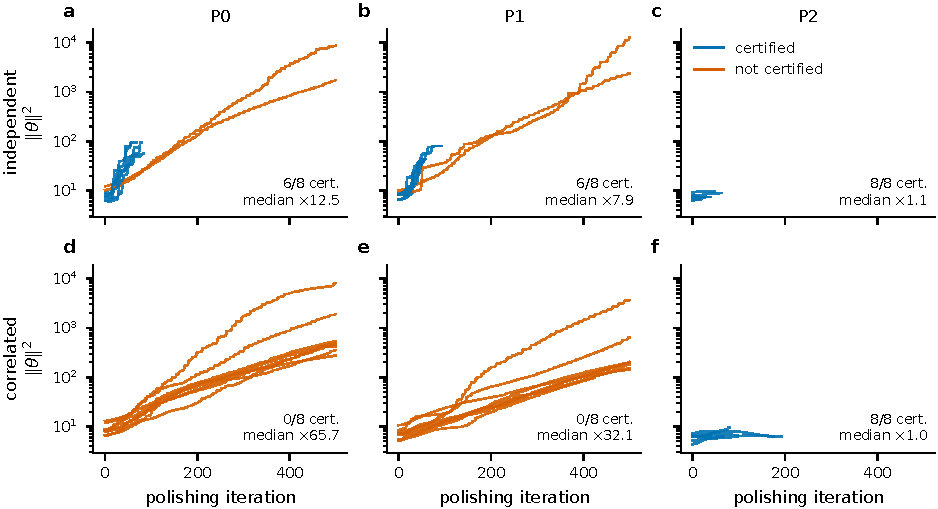
\includegraphics[width=\linewidth]{fig2_synthetic.pdf}
  % CAPTION-DRAFT: review (numbers from paper2/figures/fig2_synthetic.json)
  \caption{Synthetic $2\times3$ study: $\|\theta\|^2$ over trust-exact polishing iterations (log scale), one line per seed, coloured certified (blue) or not certified (vermillion). Rows: independent and correlated inputs; columns: P0, P1, P2. Per panel, certified seeds and median growth (polished over early-stopped): independent P0: 6/8 certified, $\times$12.5; independent P1: 6/8 certified, $\times$7.9; independent P2: 8/8 certified, $\times$1.1; correlated P0: 0/8 certified, $\times$65.7; correlated P1: 0/8 certified, $\times$32.1; correlated P2: 8/8 certified, $\times$1.0.}
  \label{fig:synthetic}
\end{figure}

\textbf{Where the runaway lives.} A post-hoc anatomy of the parameter change shows that in the correlated cells almost all growth sits in the output layer: the layer-1 share of the change was 0.110 (P0) and 0.024 (P1) (Figure~\ref{fig:where}a). It went into the affine part of the output edges' RBF coefficients and, under P0, into their SiLU weights. Cancellation across the edges entering the output rose from about 1.9 to 3.1--3.2, and no hidden unit saturated. The two uncertified independent-P0 seeds put 99.4\% of their change into the output layer. This is Step 4 of Section 3. Among independent-input models, those that ran away were exactly those whose hidden units had become correlated (largest pairwise correlation 0.70, against 0.05 for certified models; Figure~\ref{fig:where}b), while certified P2 models kept correlations up to 0.88 without running away (post-hoc).


\begin{figure}[t]
  \centering
  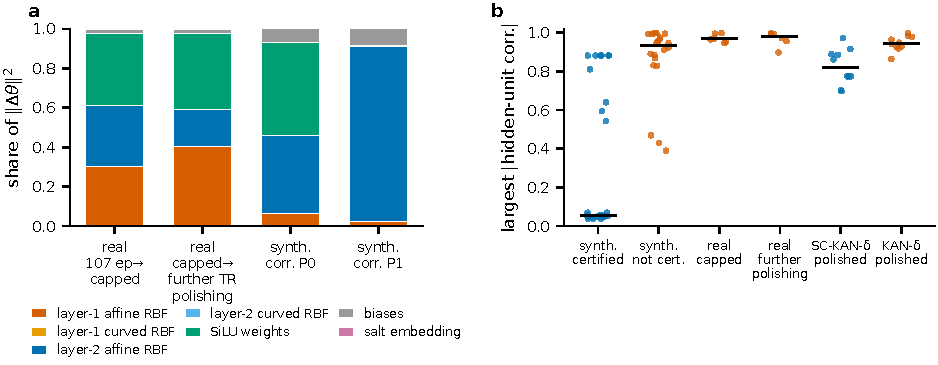
\includegraphics[width=\linewidth]{fig4_where.pdf}
  % CAPTION-DRAFT: review (numbers from paper2/figures/fig4_where.json)
  \caption{Where the runaway lives. \textbf{(a)} Mean share of $\|\Delta\theta\|^2$ by parameter block. Real data, 107 epochs$\to$capped: layer-1 affine RBF 0.30, layer-2 affine RBF 0.31, SiLU weights 0.37; capped$\to$Part~A: 0.40, 0.19, 0.38; synthetic correlated P0: layer-2 affine RBF 0.39, SiLU weights 0.47; correlated P1: layer-2 affine RBF 0.89. The real-data split was evaluated post hoc from archived weights (Appendix~\ref{app:repro}). \textbf{(b)} Largest absolute correlation between hidden-unit activations on the training rows, median: synth. certified 0.054 ($n=28$); synth. not cert. 0.935 ($n=20$); real capped 0.968 ($n=6$); real Part A 0.983 ($n=6$); SC-KAN-$\delta$ polished 0.818 ($n=10$); KAN-$\delta$ polished 0.946 ($n=10$). Blue: certified; vermillion: not certified or runaway.}
  \label{fig:where}
\end{figure}

\textbf{Verdicts.} Of six pre-registered predictions, one held (the certification pattern, X2) and five failed. The failures refine rather than contradict the mechanism. Independent cells exceeded the growth threshold, mostly through finite growth. Cancellation and extrapolation effects were weaker than predicted. Recoverability failed only because the runaway cells were more recoverable than predicted, not less. In this synthetic setting, polishing did not degrade extrapolation: most of the off-pattern error in correlated cells was present at early stopping.

\section{Real-data case study: electrolyte conductivity}\label{sec:5}

\textbf{Task and model.} The CALiSol-23 challenge \citep{deblasio2024calisol} asks for the log conductivity of lithium-ion electrolytes; every test sample contains diethyl carbonate (DEC), which never appears in training. KAN-delta anchors each prediction on the measured conductivity of pure propylene carbonate (PC) and learns only the correction, $\log k = \log k_{\mathrm{PC}} + x_{\mathrm{co}}\, h(z)$, where h is a FastKAN-style network of shape [10, 6, 1]. Its inputs are physical descriptors of the solvents (dielectric constant, log viscosity, molar mass), temperature, molality and a salt embedding. A second-difference penalty acts on the RBF coefficients, and the SiLU weights are unpenalised. Early-stopped after 107 AdamW epochs, it reached RMSE 0.142 on a held-out co-solvent.

\textbf{The inputs are correlated and few-valued.} The three co-solvent descriptors take only 30 distinct combinations in training, and dielectric constant and log viscosity correlate at r = 0.966.

\textbf{Nothing ever converged.}

\begin{itemize}
  \item Of 190 pairs of polished independent seeds, none computed the same function.
  \item After 20,000 float64 L-BFGS iterations, 0 of 26 models converged; exact-Hessian trust-region methods also failed on every seed.
  \item Students trained on a frozen teacher matched its predictions (correlation 0.9988) but not its hidden units (0.66).
\end{itemize}

\textbf{The anatomy matches Section 3.}

\begin{itemize}
  \item From early stopping to the capped state, the squared parameter norm grew 150--1550$\times$ while the smoothness penalty fell 8--88$\times$.
  \item At least 99.9\% of the coefficient change during exact-Newton polishing lay in the penalty's affine null space, in 9 of 9 models.
  \item Cancellation within an edge (SiLU against RBF) stayed small, 1.13--1.33. Cancellation across the edges entering a unit rose from 1.7--2.9 to 4--10, consistent with the correlated descriptors.
  \item The runaway spread across both layers: 30--40\% of the parameter change went into layer-1 affine RBF coefficients, 37--38\% into SiLU weights and 19--31\% into layer-2 affine coefficients (post-hoc), and 12--39\% of hidden units saturated. In the synthetic runaway the output layer dominated.
\end{itemize}

\textbf{Extrapolation suffered.} Polishing beyond early stopping, under a weak null-space penalty, raised the held-out RMSE from 0.142 to 1.03. The cancelling components appear to stop cancelling on the unseen co-solvent, whose descriptors sit off the training correlation pattern. This degradation was much stronger than in the synthetic study, where correlation itself caused most of the off-pattern error; the real model was larger, its norms grew further, and the test solvent lay at the edge of the descriptor range.

\section{Closing the blind spot, and what remains}\label{sec:6}

\textbf{Dose-response on real data.} Adding $\mu Q$ (with the SiLU weights included in Q) and polishing from the early-stopped weights:

\begin{table}[t]
  \centering
  % CAPTION-DRAFT: review
  \caption{Dose-response in $\mu$ on real data (seeds).}
  \label{tab:dose}
  \small
  \begin{tabular}{l l p{0.18\linewidth} l p{0.16\linewidth}}
  \toprule
  $\mu$ & Seeds at a numerical minimum & Negative curvature (seeds) & Norm growth (seeds) & Training fit vs runaway \\
  \midrule
  $10^{-6}$ & 0 of 6 & up to 9 eigenvalues & 21--31$\times$ & about equal \\
  $10^{-5}$ & 4 of 6 & up to 4 eigenvalues & 9--43$\times$ & 12--22\% worse \\
  $10^{-4}$ & 6 of 6 & none & 1.6--16$\times$ & 15--39\% worse \\
  \bottomrule
  \end{tabular}
\end{table}

Under a second-order certificate, all six seeds at $\mu$ = $10^{-4}$ were certified (Figure~\ref{fig:dose}). (The originally pre-registered criterion, which required 10 stationary iterations, proved unreachable because the optimiser stops a few iterations after reaching a minimum; the certificate was defined afterwards and is reported alongside the original verdict.) Saturation fell to at most 0.5\% and cross-edge cancellation to 2.2--2.9.


\begin{figure}[t]
  \centering
  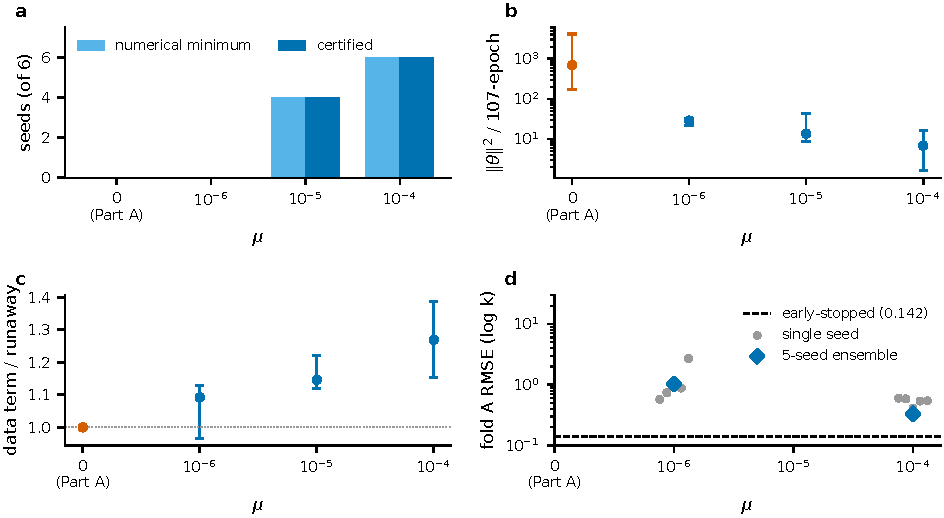
\includegraphics[width=\linewidth]{fig3_dose_response.pdf}
  % CAPTION-DRAFT: review (numbers from paper2/figures/fig3_dose_response.json)
  \caption{Real-data dose-response in the null-space weight $\mu$ (6 KAN-delta seeds; $\mu = 0$ is the runaway reference, stage-2 Part~A). \textbf{(a)} Seeds at a numerical minimum / certified: 0: 0/0; 1e-06: 0/0; 1e-05: 4/4; 0.0001: 6/6. \textbf{(b)} $\|\theta\|^2$ relative to the 107-epoch state, median (range): 0: 690.0 (170.0--4145.5); 1e-06: 28.8 (21.2--31.5); 1e-05: 13.6 (8.6--43.1); 0.0001: 6.8 (1.6--16.0). \textbf{(c)} Training data term relative to the runaway, median: 1e-06: 1.092; 1e-05: 1.146; 0.0001: 1.269. \textbf{(d)} Fold A RMSE: early-stopped 0.142 (dashed line); polished 5-seed ensemble 1.026 at $\mu = 10^{-6}$ and 0.334 at $\mu = 10^{-4}$; grey points are single seeds.}
  \label{fig:dose}
\end{figure}

\textbf{A known solution becomes recoverable.} Under the regularised loss, the original teacher is no longer a minimum. Optimising it under the same loss gives a "regularised teacher" computing nearly the same function (correlation 0.9992). Students match its units at 0.87--0.90 and its edges at 0.97--0.98, against 0.68--0.72 and 0.84--0.91 for the original teacher. This comparison was defined after the results and is exploratory.

\textbf{The penalty acts partly as gauge fixing.} At the certified minima, the layer-2 constant shift, an essentially exact symmetry, owes 96\% of its curvature to $\mu Q$: the regulariser selects one representative. The layer-1 constant shift (46\%) and unit rescaling (24\%) are only approximate symmetries in this architecture, because Gaussian bumps cannot represent constants exactly and tanh breaks rescaling.

\textbf{Convergence is not uniqueness.} Independent seeds at certified minima still disagreed: their median prediction difference fell by only 26\% (Figure~\ref{fig:uniqueness}b). With the runaway removed, the loss has several distinct isolated minima.


\begin{figure}[t]
  \centering
  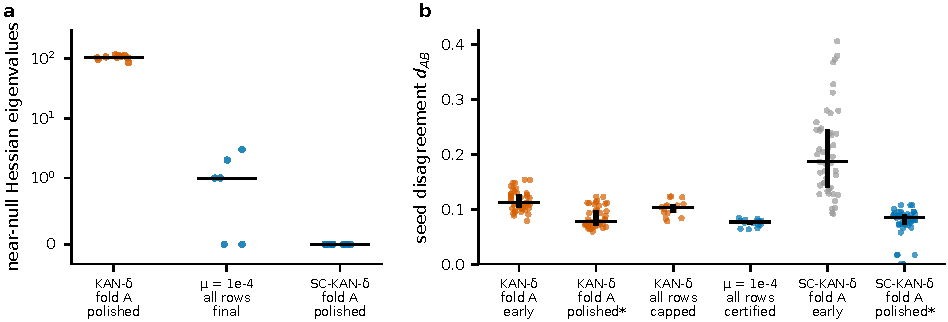
\includegraphics[width=\linewidth]{fig5_uniqueness.pdf}
  % CAPTION-DRAFT: review (numbers from paper2/figures/fig5_uniqueness.json)
  \caption{Convergence is not uniqueness. \textbf{(a)} Near-null Hessian eigenvalues ($|\lambda| < 10^{-8}\lambda_{\max}$) at the end of polishing: KAN-delta baseline on fold A, median 106 (range 86--116); null-space penalty $\mu = 10^{-4}$ on all rows, median 1 (range 0--3); SC-KAN-delta on fold A, 0--0. \textbf{The baseline counts are taken at non-stationary points}: none of the 10 baseline models was certified, and all stopped at the 500-iteration cap. \textbf{(b)} Seed disagreement $d_{AB}$ (median, interquartile range): KAN-$\delta$ fold A early 0.112; KAN-$\delta$ fold A polished$^*$ 0.077; KAN-$\delta$ all rows capped 0.104; $\mu$ = 1e-4 all rows certified 0.077; SC-KAN-$\delta$ fold A early 0.187; SC-KAN-$\delta$ fold A polished$^*$ 0.085. Groups marked $^*$ (polished fold A) are not in any committed result: they were evaluated post hoc from the archived polished weights (SHA-verified; predictions on the 1434 fold A training rows), without any re-optimisation.}
  \label{fig:uniqueness}
\end{figure}

\textbf{Extrapolation.} On the held-out co-solvent, RMSE was 0.142 for the early-stopped model, 1.026 after polishing at $\mu$ = $10^{-6}$ and 0.33 at $\mu$ = $10^{-4}$. Bounding the runaway recovers most of the damage, but early stopping remains the most accurate choice.

\textbf{Structured alternatives.} We tested two architectures designed to remove runaway routes by construction, against the early-stopped baseline, with leave-one-co-solvent-out (LOCO) validation:

\begin{table}[t]
  \centering
  % CAPTION-DRAFT: review
  \caption{Structured alternatives against the early-stopped baseline.}
  \label{tab:alternatives}
  \small
  \begin{tabular}{l p{0.24\linewidth} l l p{0.16\linewidth}}
  \toprule
  Model & Idea & LOCO RMSE & Converged & Seed agreement \\
  \midrule
  Baseline KAN-delta & As above & 0.255 & 0/10 & 0.112 \\
  Shared-curve KAN & One curve per input, mixed by penalised weights & 0.292 & 10/10 & 0.187 early; 0.085 polished \\
  Two-anchor excess model & Pure-solvent offset plus $x(1 - x)$ mixing term & 0.283 & not tested & not tested \\
  \bottomrule
  \end{tabular}
\end{table}

Seed agreement is the median prediction difference between seeds (lower is better). The shared-curve model converged every time, ending with no near-flat directions where the baseline had a median of 106 (range 86--116, at non-stationary points; Figure~\ref{fig:uniqueness}a), and it was less accurate. At the early-stopped state its seeds agreed less than the baseline's (the pre-registered comparison); after polishing to certified minima their median disagreement fell to 0.085, with some seed pairs reaching the same minimum (post-hoc). The excess model's "pure co-solvent offset" tracked viscosity rather than dielectric constant (rank correlation $-$0.85, post hoc), reflecting that no training row contains a pure co-solvent.

\section{Recommendations for practitioners}\label{sec:7}

\begin{enumerate}
  \item \textbf{Penalise the affine null space and the SiLU weights.} If a KAN uses a second-difference or curvature penalty, add a small penalty on the constant-plus-linear component of each edge's coefficients and on each SiLU weight, in every layer. Calibrate its weight so it barely moves a known smooth solution.
  \item \textbf{Check input correlations, including between hidden units.} Strongly correlated or few-valued inputs make the first layer vulnerable; any hidden layer can expose the next one.
  \item \textbf{Monitor parameter norms, not only the loss.} Steady norm growth with a slowly falling loss and stubborn gradients is the signature of the runaway. Certify convergence with a second-order criterion rather than assuming it.
  \item \textbf{Do not read edges from unconverged models.} Compare edges across seeds only after removing exact gauge freedoms, and only for models that reached certified minima.
  \item \textbf{Treat seed disagreement as information.} Even at certified minima, distinct solutions can remain. Disagreement then signals that the data do not determine the function, not merely that training was unfinished.
  \item \textbf{Validate on genuinely new conditions.} A held-out fold from the training distribution can understate extrapolation error severalfold; leave-one-group-out validation is closer to the use case.
  \item \textbf{Keep early stopping as a baseline.} In our real-data case it gave the best held-out accuracy of every variant tested.
\end{enumerate}

\section{Limitations and research process}\label{sec:8}

\textbf{Scope.}

\begin{itemize}
  \item One real dataset and one synthetic teacher; small networks ([4, 3, 1] and [10, 6, 1]).
  \item One edge type: Gaussian RBFs on fixed centres with a SiLU base. The argument applies to B-spline KANs with second-difference or curvature penalties, but we did not test them directly.
  \item Our P1 keeps the second-difference penalty on RBF coefficients and adds Bagrow's SiLU term; it is Bagrow-style, not a replication of his RBF curvature form.
  \item The null-space weight used in the shared-curve model was carried over from the synthetic calibration, not re-calibrated.
\end{itemize}

\textbf{Post-hoc elements.} The second-order certificate, the regularised-teacher comparison, the gauge-curvature analysis and both anatomy studies were defined after seeing results. We report them as exploratory and never in place of pre-registered verdicts.

\textbf{Extrapolation.} The strong degradation from polishing appeared on real data but not in the synthetic study, so we do not claim it as a general law.

\textbf{Process.} Each study committed its predictions, thresholds and interpretation rules before its code existed; any later change was dated and recorded as an amendment, and every verdict is linked to the commit that produced it. Several predictions failed or proved untestable as specified; following them up, rather than reinterpreting them, is what led to the mechanism reported here. Experiments were run with an AI coding agent working under this protocol, with a rule that committed files take precedence over any number stated in a prompt.


\bibliography{references}
\bibliographystyle{tmlr}

\appendix
\ifdefined\PREPRINT
  % GENERATED by build_tex.py (preprint: real commit hashes)
\section{All pre-registered predictions}\label{app:prereg}

Generated by \texttt{paper2/tex/build\_tex.py} from the committed verdict sections; the cell text is the committed wording. Each study opens with its pre-registration's title and its committed question (or theory). Commits are given as pre-registration $\to$ results (in the anonymous version, as neutral labels S-NN). Thresholds are part of each prediction's wording.

\subsection{Synthetic controlled study}
\noindent\textit{Pre-registration:} ``Pre-registration: synthetic teacher-student test of the runaway mechanism (paper2/synth)''. \textbf{Teacher and students: KAN [4, 3, 1].} Two stacked \texttt{kan.KANLayer}s with tanh between them, as in \texttt{kan.KAN}, but \textbf{without} the salt embedding that \texttt{kan.KAN} always adds. Same edge type: SiLU base plus 8 Gaussian RBFs on fixed centres linspace($-$1, 1, 8), width 2/7.

{\footnotesize\setlength{\tabcolsep}{3pt}
\begin{longtable}{R{0.07\linewidth} R{0.28\linewidth} R{0.35\linewidth} R{0.09\linewidth} R{0.11\linewidth}}
\toprule
ID & Prediction (threshold) & Result & Verdict & Commits \\
\midrule
\endhead
X1 & runaway ($\geq$ 10) in correlated P0 and P1; $\leq$ 3 in the three independent cells and correlated P2 & Correlated P0 $\times$65.7 and P1 $\times$32.1, and P2 $\times$1.00, as predicted. \textbf{But independent P0 $\times$12.5 and P1 $\times$7.9 exceed 3} (independent P2 $\times$1.09) & \textbf{failed} & dfd281d$\to$\allowbreak 34cc321 \\
X2 & certified $\leq$ 2/8 in correlated P0 and P1; $\geq$ 6/8 elsewhere & correlated P0 0/8, P1 0/8; independent 6/8, 6/8, 8/8; correlated P2 8/8 & \textbf{held} & dfd281d$\to$\allowbreak 34cc321 \\
X3 & cancellation in correlated P0 and P1 each $\geq$ 2 $\times$ correlated P2 & P0 3.29 and P1 2.32, against 2 $\times$ 1.99 = 3.98 & \textbf{failed} & dfd281d$\to$\allowbreak 34cc321 \\
X4 & off-manifold ratio $\geq$ 3 in correlated P0 and P1, $\leq$ 1.5 in P2 & P0 1.22, P1 \textbf{0.77}; P2 0.78 (the P2 part held) & \textbf{failed} & dfd281d$\to$\allowbreak 34cc321 \\
X5 & Spearman(cancellation, off-manifold RMSE) $\geq$ 0.6 over the 24 correlated models & $\rho$ = +0.177, p = 0.407 & \textbf{failed} & dfd281d$\to$\allowbreak 34cc321 \\
X6 & unit match $\geq$ 0.85 in the independent cells and correlated P2; < 0.7 in correlated P0 and P1 & The first part held: 1.000 in all four no-runaway-predicted cells. \textbf{The second part failed: correlated P0 0.774 and P1 0.883 are not < 0.7} & \textbf{failed} & dfd281d$\to$\allowbreak 34cc321 \\
\bottomrule
\end{longtable}}
\subsection{Real-data case study}
\noindent\textit{From the case-study close-out:} KAN-$\delta$ predicts Li-electrolyte conductivity for the CALiSol-23 DEC holdout. Its
prediction is log k = a measured pure-PC anchor + x\_co $\cdot$ h(solvent descriptors, 1/T, molality, salt).
Its first layer is a [8 continuous inputs + 2 salt-embedding, 6, 1] FastKAN, with SiLU + 8 Gaussian
RBFs per edge and a smoothness penalty (\texttt{kan.py}, \texttt{final.py}).

Rows are as committed in the case-study summary (one row may cover several predictions, e.g.\ F2--F5). The rank intervention's verdicts are given per arm in the result column.

{\footnotesize\setlength{\tabcolsep}{3pt}
\begin{longtable}{R{0.14\linewidth} R{0.26\linewidth} R{0.29\linewidth} R{0.10\linewidth} R{0.11\linewidth}}
\toprule
Study & Prediction (threshold) & Result & Verdict & Commits \\
\midrule
\endhead
Gauge study & \textbf{Control 1}: teacher edges recovered, median dense corr $\geq$ 0.8 & 0.301 (sanity: h corr 0.913 < 0.95) & \textbf{failed} & c11dd92$\to$\allowbreak{}e68e2eb \\
Gauge study & P1: gauge fixing removes $\geq$ 50\% of edge variance & not run & inconclusive (gated by Control 1) & c11dd92$\to$\allowbreak{}e68e2eb \\
Gauge study & P2: sparse $\geq$ 2$\times$ dense, DEC region highest & not run & inconclusive (gated) & c11dd92$\to$\allowbreak{}e68e2eb \\
Gauge study & P3: (e) < (d) < (c) < (a) & not run & inconclusive (gated) & c11dd92$\to$\allowbreak{}e68e2eb \\
Gauge study & P4: every seed has a unit with |corr| < 0.8 & not run & inconclusive (gated) & c11dd92$\to$\allowbreak{}e68e2eb \\
Gauge study & P5: KAN-full edge variance > KAN-$\delta$ & not run & inconclusive (gated) & c11dd92$\to$\allowbreak{}e68e2eb \\
Gauge study & P6: seed spread flags errors & Spearman +0.169 (A) / +0.213 (B); fold B RMSE at 80\% coverage 0.153 vs random 0.137 & \textbf{failed} & c11dd92$\to$\allowbreak{}67fe9f2 \\
Control 2 & C1: (I,C) edges $\geq$ 0.9 and units $\geq$ 0.9 & prediction corr 0.947 < 0.99 & inconclusive (gate failed) & 45b336f$\to$\allowbreak{}a260aef \\
Control 2 & C2: (R,C) invT, molal $\geq$ 0.9; co-solvent < 0.7 & prediction corr 0.969 < 0.99 & inconclusive (gate failed) & 45b336f$\to$\allowbreak{}a260aef \\
Control 2 & C3: 107 epochs gives prediction corr < 0.95 & 0.858 (I,S), 0.919 (R,S) & \textbf{held} & 45b336f$\to$\allowbreak{}a260aef \\
Control 3 & C1': (I) passes the gate, edges $\geq$ 0.9, units $\geq$ 0.9 & (I) RMSE/std 0.128 > 0.05; unit match 0.648 & \textbf{failed} & 812a0fa$\to$\allowbreak{}9f59d39 \\
Control 3 & C2': (R) edges $\leq$ (I) edges $-$ 0.10 & (R) edges 0.852, units 0.659 & inconclusive ((I) failed the gate) & 812a0fa$\to$\allowbreak{}9f59d39 \\
Control 3 & C4: every continuous input $\geq$ 0.9 in (I) & -- & inconclusive ((I) failed the gate) & 812a0fa$\to$\allowbreak{}9f59d39 \\
Fiber & F1: $\geq$ 50\% of seed pairs on-fiber & 0/190 (closest d = 0.146) & \textbf{failed} & e83df2e$\to$\allowbreak{}f220a2f \\
Fiber & F2--F5 & not run & inconclusive (no on-fiber pairs) & e83df2e$\to$\allowbreak{}f220a2f \\
Fiber 2 & G1: $\geq$ 4/6 seeds and $\geq$ 10/20 students certify convergence & 0/6, 0/20 (all at the 20,000-iteration cap) & \textbf{failed} & 4af5250$\to$\allowbreak{}98eca9d \\
Fiber 2 & G2--G5 & not run & inconclusive (no converged model) & 4af5250$\to$\allowbreak{}98eca9d \\
Support & H1: dim(N) $\geq$ 5 & dim(N) = 36 of 72 & \textbf{held} & b473232$\to$\allowbreak{}c5505e5 \\
Support & H2: $\geq$ 50\% of N is REDISTRIBUTION within the correlated group & 18/36 & \textbf{held, exactly at threshold} & b473232$\to$\allowbreak{}c5505e5 \\
Support & H3: set A fraction in N $\geq$ 0.5 and $\geq$ 3$\times$ random & median 0.942 (random 0.5) & inconclusive (untestable: 3 $\times$ 0.5 > 1) & b473232$\to$\allowbreak{}c5505e5 \\
Support & H4: set B (capped), same criterion & median 0.949 & inconclusive (untestable) & b473232$\to$\allowbreak{}c5505e5 \\
Support & H5: flattest Hessian directions overlap N $\geq$ 0.5 & median 0.885; median layer-1 block share only 0.08 & \textbf{held}, with caveat (see \texttt{support\_\allowbreak{}prereg.md}) & b473232$\to$\allowbreak{}c5505e5 \\
Support & H6: fraction in N rises from control-3 to capped state, $\geq$ 15/20 & 20/20 (0.713 $\to$\allowbreak{} 0.949) & \textbf{held} & b473232$\to$\allowbreak{}c5505e5 \\
Rule & I1--I5 (gate) & 0 columns removed; gate stopped & inconclusive & 6c93bf4$\to$\allowbreak a53cc2a \\
Rank & I1: median max|grad| $\leq$ 0.1 $\times$ baseline & arm G: \textbf{failed} (4.00$\times$); arm F: \textbf{failed} (29.1$\times$) & see result & df44ead$\to$\allowbreak aeb6f87 \\
Rank & I2: median d\_AB $\leq$ 0.5 $\times$ baseline & arm G: \textbf{failed} (0.945$\times$); arm F: \textbf{failed} (0.808$\times$) & see result & df44ead$\to$\allowbreak aeb6f87 \\
Rank & I3 (sanity): median loss $\leq$ 1.10 $\times$ baseline & arm G: passed (1.004$\times$); arm F: passed, narrowly (1.099$\times$) & see result & df44ead$\to$\allowbreak aeb6f87 \\
Rank & I4: fold A RMSE $\leq$ 0.150 (KAN-$\delta$ 0.1420) & arm G: \textbf{held}, narrowly (0.1499); arm F: \textbf{failed} (0.1587) & see result & df44ead$\to$\allowbreak aeb6f87 \\
Rank & I5: edge corr on 1000/T and molality $\geq$ baseline + 0.1 (baseline 0.102) & arm G: \textbf{held} (0.927); arm F: \textbf{held} (0.338) & see result & df44ead$\to$\allowbreak aeb6f87 \\
Rank & I6: arm F's improvement $\geq$ arm G's in both I1 and I2 & arm G: \textbf{failed} (max|grad| 29.1$\times$ vs 4.00$\times$; d\_AB does favour F, 0.808 vs 0.945) & see result & df44ead$\to$\allowbreak aeb6f87 \\
Trust & T1 / T2: trust-krylov certifies $\geq$ 4/6 seeds / $\geq$ 2/3 students & 0/6, 0/3. All 9 stopped on scipy's "bad approximation" after 1--62 iterations; the Hessian was accurate to $\leq$ $2\times10^{-7}$ & \textbf{failed} & a77e8b4$\to$\allowbreak 67586d6 \\
Trust & T3--T5 & nothing converged & inconclusive & a77e8b4$\to$\allowbreak 67586d6 \\
Stage 2 & U1: trust-exact (exact Hessian, 500 iterations) certifies $\geq$ 4/6 seeds & 0/6. All 9 hit the iteration cap & \textbf{failed} & c6a9e83$\to$\allowbreak b8d6488 \\
Stage 2 & U2: with L2 $\lambda$ = $10^{-5}$, $\geq$ 4/6 seeds and $\geq$ 2/3 students & 1/6 seeds, 0/3 students & \textbf{failed} & c6a9e83$\to$\allowbreak b8d6488 \\
Stage 2 & U3: more converge at $10^{-5}$ than at $10^{-6}$ & 1 vs 0 & \textbf{held} & c6a9e83$\to$\allowbreak b8d6488 \\
Stage 2 & U4: converged L2 models' loss without L2 $\leq$ 1.05 $\times$ capped & 1.2545 & \textbf{failed} & c6a9e83$\to$\allowbreak b8d6488 \\
Stage 2 & U5: converged seeds' disagreement $\leq$ 0.5 $\times$ capped & only 1 converged & inconclusive & c6a9e83$\to$\allowbreak b8d6488 \\
Close & V1: at some $\mu$, $\geq$ 4/6 seeds and $\geq$ 2/3 students converge (stage2 criterion) & 0 certified at every $\mu$ & \textbf{failed} & e5105d7$\to$\allowbreak{}65ed55f \\
Close & V2: converged seeds' data term $\leq$ 1.05 $\times$ stage2 A & nothing certified at the selected $\mu$ = $10^{-6}$ & inconclusive & e5105d7$\to$\allowbreak{}65ed55f \\
Close & V3: $\|\theta\|^{2}$ $\leq$ 10 $\times$ start & same & inconclusive & e5105d7$\to$\allowbreak{}65ed55f \\
Close & V4: seed disagreement halved & same & inconclusive & e5105d7$\to$\allowbreak{}65ed55f \\
Close & V5: students' unit match $\geq$ 0.8 & same & inconclusive & e5105d7$\to$\allowbreak{}65ed55f \\
Close & V6: fold A RMSE $\leq$ 0.150 & 1.0262, bias +0.9028 & \textbf{failed} & e5105d7$\to$\allowbreak{}65ed55f \\
Certify & W1: at $\mu$ = $10^{-4}$, $\geq$ 5/6 seeds certified (second-order criterion, F-a) & 6/6; all 17 candidates certified & \textbf{held} & 5f4520a$\to$\allowbreak{}36f295b \\
Certify & W2: certified seeds' median d\_AB $\leq$ 0.5 $\times$ capped & 0.0771 vs capped 0.1041 ($-$26\%) & \textbf{failed} & 5f4520a$\to$\allowbreak{}36f295b \\
Certify & W3: certified students' unit match $\geq$ 0.8 (vs the original teacher) & 0.624 & \textbf{failed} & 5f4520a$\to$\allowbreak{}36f295b \\
Certify & W4: $\mu$ = $10^{-4}$ fold A RMSE $\leq$ 0.150 & 0.3345 & \textbf{failed} & 5f4520a$\to$\allowbreak{}36f295b \\
Certify & W5: $\mu$ = $10^{-4}$ fold A RMSE $\leq$ 0.5131 & 0.3345 & \textbf{held} & 5f4520a$\to$\allowbreak{}36f295b \\
Certify & W6: Spearman(cross-edge ratio, held-out RMSE) $\geq$ 0.6 & $\rho$ = +0.345, p = 0.328 (weak test) & \textbf{failed} & 5f4520a$\to$\allowbreak{}36f295b \\
\bottomrule
\end{longtable}}
\noindent Committed tally of the case study:

{\footnotesize\setlength{\tabcolsep}{3pt}
\begin{longtable}{R{0.55\linewidth} r r r}
\toprule
Study & Held & Failed & Inconclusive \\
\midrule
\endhead
First table (Control 1, P1--P6, C1--C3, C1'/C2'/C4, F1--F5, G1--G5, H1--H6) & 5 & 5 & 19 \\
Rule (I1--I5) & 0 & 0 & 5 \\
Rank (I1, I2, I4, I5 per arm, I6) & 3 & 6 & 0 \\
Trust (T1--T5) & 0 & 2 & 3 \\
Stage 2 (U1--U5) & 1 & 3 & 1 \\
Close (V1--V6) & 0 & 2 & 4 \\
Certify (W1--W6) & 2 & 4 & 0 \\
\textbf{Total} & \textbf{11} & \textbf{22} & \textbf{32} \\
\bottomrule
\end{longtable}}
\subsection{Shared-curve KAN}
\noindent\textit{Pre-registration:} ``SC-KAN-$\delta$ (shared-curve KAN-$\delta$): pre-registration''. \textbf{Inputs:} the 8 continuous final.py features (flag 11), scaled exactly as in final.py. Salt enters through a learned 2-number embedding e(salt), passed through tanh.

Run after the case-study close-out; not part of the 65 predictions above.

{\footnotesize\setlength{\tabcolsep}{3pt}
\begin{longtable}{R{0.07\linewidth} R{0.28\linewidth} R{0.35\linewidth} R{0.09\linewidth} R{0.11\linewidth}}
\toprule
ID & Prediction (threshold) & Result & Verdict & Commits \\
\midrule
\endhead
S1 & SC LOCO RMSE $\leq$ 1.05 $\times$ baseline & unweighted mean SC 0.2923 vs base 0.2554 (ratio 1.145; threshold 0.2681). Also reported: row-weighted 0.2478 / 0.2297 (1.079); folds $\geq$ 20 rows 0.3138 / 0.2093 (1.499) & failed & 0053d01$\to$\allowbreak e00e37f \\
S2 & SC fold A RMSE $\leq$ 0.160 & SC 0.1757 (base 0.1420) & failed & 0053d01$\to$\allowbreak e00e37f \\
S3 & SC median d\_AB $\leq$ 0.5 $\times$ baseline & SC 0.1865 vs base 0.1120 (threshold 0.0560): SC seeds agree \emph{less} than baseline seeds & failed & 0053d01$\to$\allowbreak e00e37f \\
S4 & curve corr $\geq$ 0.90 for $\geq$ 6 of 8 inputs & 3 of 8 (M\_co 0.959, mix\_lneta 0.970, invT 0.986); lowest x\_co 0.596; others 0.871--0.891 & failed & 0053d01$\to$\allowbreak e00e37f \\
S5 & $\geq$ 8/10 SC fold A models certified & SC 10/10 (max|grad| $\leq$ $7\times10^{-10}$, 0 near-null eigenvalues); baseline 0/10 (all hit the 500-iteration cap) & held & 0053d01$\to$\allowbreak e00e37f \\
S6 & median $\beta$-norm polished/early $\leq$ 3 (calibrated) & median 1.337 (range 0.652--2.356); $\|\theta\|^{2}$ $\times$4.59 (base $\times$67.9, range 30.6--281) & held & 0053d01$\to$\allowbreak e00e37f \\
S7 & SC polished/early fold A RMSE $\leq$ 1.5 & SC 1.920 (0.1757 $\to$\allowbreak{} 0.3373); baseline 5.736 (0.1420 $\to$\allowbreak{} 0.8147) & failed & 0053d01$\to$\allowbreak e00e37f \\
S8 & d log k/d(1000/T) < 0 on $\geq$ 95\% rows in $\geq$ 8/10 seeds & 10/10 (median share 1.000; 1424 rows, 10 excluded per D4) & held & 0053d01$\to$\allowbreak e00e37f \\
S9 & Spearman(1000/T, |slope|) > 0 in $\geq$ 8/10 seeds & 10/10 (median +0.661, range +0.406 to +0.885) & held & 0053d01$\to$\allowbreak e00e37f \\
S10 & d log k/d(ln $\eta$\_mix) < 0 on $\geq$ 90\% rows in $\geq$ 8/10 seeds & 7/10 (median share 0.967; s0 0.892, s2 0.892, s8 0.826) & failed & 0053d01$\to$\allowbreak e00e37f \\
\bottomrule
\end{longtable}}
\subsection{Two-anchor excess model}
\noindent\textit{Pre-registration:} ``EX-KAN (two-anchor excess model): pre-registration''. log k = anchor\_PC + x\_co $\cdot$ s(eps\_co, ln\_eta\_co, M\_co, 1000/T) + x\_co $\cdot$ (1 $-$ x\_co) $\cdot$ g(eps\_co, ln\_eta\_co, M\_co, 1000/T, molality, salt) So $\delta$ = log k $-$ anchor\_PC = x\_co $\cdot$ [s + (1 $-$ x\_co) $\cdot$ g].

Run after the case-study close-out; not part of the 65 predictions above.

{\footnotesize\setlength{\tabcolsep}{3pt}
\begin{longtable}{R{0.07\linewidth} R{0.28\linewidth} R{0.35\linewidth} R{0.09\linewidth} R{0.11\linewidth}}
\toprule
ID & Prediction (threshold) & Result & Verdict & Commits \\
\midrule
\endhead
E1 & EX LOCO $\leq$ 0.95 $\times$ KAN-$\delta$ & unweighted mean EX 0.2834 vs threshold 0.2426 (base 0.2554; ratio 1.110). Row-weighted 0.2363 / 0.2297 (1.029); folds $\geq$ 20 rows 0.2662 / 0.2093 (1.272). EX is better on EC (0.237 vs 0.256), Sulfolane, 3-Glyme, 2-Glyme and Toluene, and worse on 2-MeTHF, THF, Methylene chloride, DME and EA & failed & 3938f8f$\to$\allowbreak 579b58f \\
E2 & EX fold A $\leq$ 0.142 & EX 0.1502 (base this run 0.1420) & failed & 3938f8f$\to$\allowbreak 579b58f \\
E3 & s agrees across seeds (separable co-solvents, Amendment 1) & median pairwise corr +0.987 over EA, EC, Methylene chloride: a weak test with 3 values per seed, and Methylene chloride is marginal. Seed SD of s: EA 0.063 (0.39 $\times$ the spread across co-solvents, 0.159), EC 0.091 (0.57 $\times$), Methylene chloride 0.067 (0.42 $\times$). Secondary ($\leq$ 2 rule, 7 co-solvents): +0.869 & held & 3938f8f$\to$\allowbreak 579b58f \\
E4 & mean s(low $\varepsilon$) < mean s(EC, Sulfolane) in $\geq$ 8/10 seeds & 0/10: the ordering is reversed in every seed. Per high-$\varepsilon$ co-solvent: vs EC alone 0/10 (EC median s +0.104), vs Sulfolane alone 0/10 (median $-$0.124). The low-$\varepsilon$ mean is +0.19 to +0.49 per seed. Sulfolane does not drive the failure on its own: EC alone fails in every seed too & failed & 3938f8f$\to$\allowbreak 579b58f \\
E5 & median seed-SD flagged $\geq$ 2 $\times$ separable (Amendment 1) & 0.091 vs 0.067, ratio 1.37. Secondary ($\leq$ 2 rule): 0.222 vs 0.069, ratio 3.22, no verdict; the secondary is driven by 3-Glyme (SD 0.478, M\_co extrapolated) and 2-Glyme (0.222) & failed & 3938f8f$\to$\allowbreak 579b58f \\
\bottomrule
\end{longtable}}
\paragraph{Revision studies.} The studies below were run for the revision, each with its own pre-registration.

\subsection{Freeze test: is composition necessary? (and weight decay)}
\noindent\textit{Pre-registration:} ``Revision step 2: is composition necessary? (plus weight decay)''. With layer 1 fixed, the output is linear in the layer-2 parameters: a fixed basis times coefficients. The data term plus a quadratic penalty is then a convex quadratic. It can have flat directions but no tilted ones, so it cannot run away. If the runaway needs composition, freezing layer 1 should remove it.

{\footnotesize\setlength{\tabcolsep}{3pt}
\begin{longtable}{R{0.07\linewidth} R{0.28\linewidth} R{0.35\linewidth} R{0.09\linewidth} R{0.11\linewidth}}
\toprule
ID & Prediction (threshold) & Result & Verdict & Commits \\
\midrule
\endhead
Z1 & Arm A certified: $\geq$ 5/6 real; $\geq$ 7/8 in each synthetic cell & A-R 6/6; A-S correlated P0 8/8; A-S correlated P1 8/8 & HELD & a6d752b$\to$\allowbreak 9228f70 \\
Z2 & Arm A median layer-2 growth $\leq$ 3 in R and in each synthetic cell & A-R $\times$582.8 ($\times$206--$\times$11,689); P0 $\times$4.07 ($\times$1.36--$\times$245); P1 $\times$22.9 ($\times$1.51--$\times$801) & FAILED & a6d752b$\to$\allowbreak 9228f70 \\
Z3 & Arm A smallest Hessian eigenvalue $\geq$ $-10^{-8}$ $\times$ largest at every logged iterate & worst ratio +$1.99\times10^{-10}$ (all values positive) & HELD & a6d752b$\to$\allowbreak 9228f70 \\
Z4 & Arm C: 8/8 certified, median growth $\leq$ 3 & 8/8; $\times$2.52 ($\times$1.68--$\times$2.85) & HELD (computed before the stop) & a6d752b$\to$\allowbreak 9228f70 \\
Z5 & Arm D branch & 8/8 certified; median growth $\times$0.415 ($\times$0.263--$\times$0.540). Note: this rule uses the same $\leq$ 3 growth threshold as Z2 and shares its weakness (see the interpretation note); here the norm shrinks, so the threshold is not binding. & "an L2 term of this size at polish time bounds the runaway" & a6d752b$\to$\allowbreak 190544d \\
Z6 E(i) & Arm E, synthetic correlated P0 & median $\|\theta\|^{2}$ ratio wd 0 / wd $10^{-4}$ $\times$1.0011 ($\times$0.987--$\times$1.007); in-distribution RMSE 0.0091 vs 0.0091; off-manifold 0.0667 vs 0.0665; determinism check max |diff| 0 & "early stopping alone kept them bounded; weight decay was incidental" & a6d752b$\to$\allowbreak 190544d \\
Z6 E(ii) & Arm E, real fold A & median ratio $\times$1.0001 ($\times$1.0001--$\times$1.0001); fold A ensemble RMSE 0.1420 vs 0.1420; determinism check max |diff| 0 & "early stopping alone kept them bounded; weight decay was incidental" & a6d752b$\to$\allowbreak 190544d \\
\bottomrule
\end{longtable}}
\subsection{Infimum test: a certified regularisation path}
\noindent\textit{Pre-registration:} ``Revision step 3: infimum test (a certified L2 regularisation path)''. Does the unregularised loss of the full model have a finite minimum that is merely distant? Or does its infimum lie at infinity (a receding minimum)?

Predictions I1--I4 apply per phase (Phase 1 synthetic, Phase 2 real data); the real-data control arm was added after Phase 2 with its outcomes fixed before it ran.

{\footnotesize\setlength{\tabcolsep}{3pt}
\begin{longtable}{R{0.07\linewidth} R{0.28\linewidth} R{0.35\linewidth} R{0.09\linewidth} R{0.11\linewidth}}
\toprule
ID & Prediction (threshold) & Result & Verdict & Commits \\
\midrule
\endhead
I1 & Phase 1: runaway: $\|\theta^{*}\|^{2}$ increases as $\gamma$ decreases & 16/16 & HELD & 179814f$\to$\allowbreak ef3b3c2 \\
I2 & Phase 1: runaway: $\alpha$ > 0.2, bootstrap 95\% interval excluding 0 & 16/16 & HELD & 179814f$\to$\allowbreak ef3b3c2 \\
I3 & Phase 1: control: ratio between the two smallest certified $\gamma$ $\leq$ 1.5 & 8/8 & HELD & 179814f$\to$\allowbreak ef3b3c2 \\
I4 & Phase 1: runaway: $L^{*}$ decreases as $\gamma$ decreases & 16/16 & HELD & 179814f$\to$\allowbreak ef3b3c2 \\
I1 & Phase 2: runaway: $\|\theta^{*}\|^{2}$ increases as $\gamma$ decreases & 6/6 & HELD & 179814f$\to$\allowbreak 349022b \\
I2 & Phase 2: runaway: $\alpha$ > 0.2, bootstrap 95\% interval excluding 0 & 6/6 & HELD & 179814f$\to$\allowbreak 349022b \\
I3 & Phase 2: discrimination check & --- & Phase 1's I3 (HELD, 8/8), as pre-registered; Phase 2 has no control models & 179814f$\to$\allowbreak 349022b \\
I4 & Phase 2: runaway: $L^{*}$ decreases as $\gamma$ decreases & 6/6 & HELD & 179814f$\to$\allowbreak 349022b \\
Control & Post hoc, outcomes fixed before running. Plateau: the $\|\theta^{*}\|^{2}$ ratio between the two smallest certified (incl. certified-degenerate) $\gamma$ values is $\leq$ 1.5 for both seeds. The real-data contrast is then complete. & The $\|\theta^{*}\|^{2}$ ratio between the two smallest certified $\gamma$ is 1.092 (ind0) and 1.101 (ind1), both $\leq$ 1.5, so the real-data contrast is complete. The divergence condition is not met: $\alpha$ is +0.105 [+0.093, +0.118] and +0.124 [+0.109, +0.139], both below 0.2. & plateau & 349022b$\to$\allowbreak 4003b21 \\
\bottomrule
\end{longtable}}
\subsection{Correlation dose-response}
\noindent\textit{Pre-registration:} ``Revision step 4: dose-response --- how much correlation does the blind spot need?''. At what input correlation does the runaway turn on, and does the null-space penalty still close it at the strongest dose?

Verdict column: P0 / P1. The thresholds are synthetic ([4, 3, 1], Gaussian inputs), not real-data thresholds.

{\footnotesize\setlength{\tabcolsep}{3pt}
\begin{longtable}{R{0.07\linewidth} R{0.28\linewidth} R{0.35\linewidth} R{0.09\linewidth} R{0.11\linewidth}}
\toprule
ID & Prediction (threshold) & Result & Verdict & Commits \\
\midrule
\endhead
R1 & The uncertified fraction (measure 1) is non-decreasing across $\rho$, for P0 and for P1 separately, allowing one inversion. & P0: HELD: 0.125, 0.625, 0.500, 1, 1, 1 (1 inversion); P1: HELD: 0.125, 0.500, 0.500, 0.625, 1, 1 (0 inversions) & held / held & 1a18569$\to$\allowbreak 541355a \\
R2 & Control, P2 at $\rho$ = 0.99: at least 7 of 8 certified (including certified-degenerate), and median D $\leq$ 1.5. & P2 at $\rho$ = 0.99: 8/8 certified, median D 1.127 (range of growth $\times$0.88--$\times$1.11). & held & 1a18569$\to$\allowbreak 541355a \\
R3 & The median affine-RBF share of the polished change is non-decreasing in $\rho$, for P0 and for P1 (one inversion allowed). & P0: FAILED: 0.715, 0.594, 0.612, 0.476, 0.394, 0.585 (3 inversions); P1: FAILED: 0.944, 0.982, 0.748, 0.934, 0.914, 0.952 (2 inversions) & failed / failed & 1a18569$\to$\allowbreak 541355a \\
R4 & Median D increases with $\rho$, for P0 and for P1: Spearman correlation $\geq$ 0.8 between $\rho$ and the cell median D over the 6 levels. (Spearman $\geq$ 0.8 is the operative criterion; it tolerates up to about two inversions.) & P0: FAILED: D 8.01, 15.05, 6.43, 9.52, 16.13, 16.72; Spearman +0.714; P1: FAILED: D 4.54, 4.88, 2.91, 3.00, 4.52, 14.54; Spearman +0.143 & failed / failed & 1a18569$\to$\allowbreak 541355a \\
 & R4, certified-only variant & P0: FAILED (Spearman +0.714; D at 0.99 is 19.55, n = 4); P1: FAILED (Spearman +0.143) & failed / failed & 1a18569$\to$\allowbreak 541355a \\
\bottomrule
\end{longtable}}
\subsection{B-spline replication}
\noindent\textit{Pre-registration:} ``Revision step 5: B-spline replication of the synthetic 2 $\times$ 3 study''. Are the runaway and its fix a property of KAN-style edges with second-difference penalties, or an artefact of the Gaussian-RBF basis?

Step 1 verdicts at the frozen $\mu = 10^{-6}$, then the post-hoc follow-up checks whose predictions and readings were fixed before computing (check 3 is descriptive; Appendix~\ref{app:posthoc}).

{\footnotesize\setlength{\tabcolsep}{3pt}
\begin{longtable}{R{0.07\linewidth} R{0.28\linewidth} R{0.35\linewidth} R{0.09\linewidth} R{0.11\linewidth}}
\toprule
ID & Prediction (threshold) & Result & Verdict & Commits \\
\midrule
\endhead
B1 & Correlated P0 and correlated P1: at most 2 of 8 certified, each. & correlated P0: 0/8 (8 iteration cap) & HELD & 5491481$\to$\allowbreak f0accc0 \\
 &  & correlated P1: 0/8 (8 iteration cap) & HELD & 5491481$\to$\allowbreak f0accc0 \\
B2 & P2, both input conditions: at least 7 of 8 certified AND median D $\leq$ 1.5, each. & independent P2: 8/8, D 1.222 (certified-only 1.222) & HELD & 5491481$\to$\allowbreak f0accc0 \\
 &  & correlated P2: 8/8, D \textbf{2.225} (certified-only 2.225) & FAILED (the D leg; certification held) & 5491481$\to$\allowbreak f0accc0 \\
B3 & Independent P0 and P1: at least 6 of 8 certified, each (the Gaussian reference level). & independent P0: 5/8 (3 iteration cap) & FAILED & 5491481$\to$\allowbreak f0accc0 \\
 &  & independent P1: 4/8 (3 iteration cap, 1 solver error via the watchdog) & FAILED & 5491481$\to$\allowbreak f0accc0 \\
Check 1 & Post hoc, predictions fixed in advance; P2 path extended to $\gamma$ = $10^{-9}$: median D' $\leq$ 1.5 in both conditions;; median norm ratio $\|\theta^{*}$($10^{-9}$)$\|$ / $\|\theta$\_polish$\|$ within [0.9, 1.1] in both conditions. & independent: D' 1.003, norm ratio 1.000; correlated: D' 1.035, norm ratio 0.911 & both hold & ff5bd20$\to$\allowbreak 9167740 \\
Check 2 & Post hoc, prediction fixed in advance; P2 at $\mu$ = $10^{-5}$: $\geq$ 7/8 certified and median D $\leq$ 1.5 in both conditions. & independent: 8/8 certified, median D 1.167 (1.167); correlated: 8/8 certified, median D 1.309 (1.309) & held / held & ff5bd20$\to$\allowbreak 9167740 \\
\bottomrule
\end{longtable}}% GENERATED by build_tex.py (preprint: real commit hashes)
\section{Post-hoc analyses}\label{app:posthoc}

Every analysis below was defined after seeing results. Each is labelled \textbf{post hoc} in its own files, changes no pre-registered verdict, and is reported as exploratory. The description is the subject line of the commit that added the analysis.

{\footnotesize\setlength{\tabcolsep}{3pt}\begin{longtable}{R{0.28\linewidth} R{0.52\linewidth} R{0.10\linewidth}}
\toprule
Analysis & Commit subject (as committed) & Commit \\
\midrule
\endhead
\textbf{Post hoc.} Anatomy of the real-data runaway \newline \footnotesize{\texttt{anatomy\_plan.md, anatomy.py, anatomy\_output.txt}} & Plan for descriptive runaway anatomy (before anatomy.py exists) & 256b00a \\
 & Anatomy (descriptive): Q1, Q2 not as expected, Q3 as expected; RBF growth is in the penalty null space & a791652 \\
\textbf{Post hoc.} Gauge check and regularised teacher (exploratory) \newline \footnotesize{\texttt{gaugecheck.py, gaugecheck\_notes.md, gaugecheck\_output.txt}} & gaugecheck (POST-HOC, exploratory): penalty fixes gauge position by slope balance; students match the regularised teacher & 0b29351 \\
\textbf{Post hoc.} Anatomy of the synthetic runaway \newline \footnotesize{\texttt{paper2/anatomy\_synth.py, paper2/anatomy\_synth\_output.txt}} & paper2 anatomy\_synth (POST-HOC, descriptive): synthetic runaway lives mainly in layer-2 output-edge cancellation, unsaturated; no verdicts change & ea22a56 \\
\textbf{Post hoc.} Loss decomposition along the runaway \newline \footnotesize{\texttt{paper2/lossdecomp.py, paper2/lossdecomp\_output.txt}} & paper2 lossdecomp (POST-HOC, descriptive): synthetic runaway loss decrease shared, D2 penalty median 0.61 vs data 0.37; 12/20 runaway models overfit; real-data reference recomputed & 4ec6fce \\
\textbf{Post hoc.} Descriptive checks (hidden-unit correlation, tilt affinity, references) \newline \footnotesize{\texttt{paper2/checks/plan.md, paper2/checks/checks.py, paper2/checks/checks\_output.txt}} & paper2/checks: plan for descriptive checks (F4 hidden-unit correlation, F2 tilt affinity, A1 commit and data citation) before checks.py exists & 5745103 \\
 & paper2/checks (POST-HOC, descriptive): hidden-unit correlation marks the runaway (independent cells 0.70 vs 0.05) but is not sufficient; RBF tilt affine to 2\% centrally, 13\% at the ends; A1 commit 3081cc0; CALiSol-23 citation not in competition material & 6e1df32 \\
\textbf{Post hoc.} Regularised teacher (weights pinned) & Pin gaugecheck regularised-teacher weights in a seventh archive; append to weights manifest & 47d7327 \\
\bottomrule
\end{longtable}}% GENERATED by build_tex.py (preprint: real commit hashes)
\section{Reproducibility map}\label{app:repro}

Generated from \texttt{paper2/figures/MANIFEST.md}. Every figure is rebuilt by its script from committed results; each figure's sidecar JSON lists the data files (path, commit, SHA-256), any archived weights (SHA-256, archive) and every plotted number. \REPOSTATEMENT

{\footnotesize\setlength{\tabcolsep}{3pt}
\begin{longtable}{R{0.15\linewidth} R{0.13\linewidth} R{0.42\linewidth} R{0.19\linewidth}}
\toprule
Figure & Script & Data files (commit) & Archived weights \\
\midrule
\endhead
Figure~\ref{fig:mechanism} \figname{fig1\_\allowbreak{}mechanism} & \texttt{make\_\allowbreak{}fig1.py} & none (computed from committed code: kan.py, paper2/synth.py) & --- \\
Figure~\ref{fig:synthetic} \figname{fig2\_\allowbreak{}synthetic} & \texttt{make\_\allowbreak{}fig2.py} & \texttt{paper2/\allowbreak{}synth\_\allowbreak{}results.json} (34cc321) & --- \\
Figure~\ref{fig:dose} \figname{fig3\_\allowbreak{}dose\_\allowbreak{}response} & \texttt{make\_\allowbreak{}fig3.py} & \texttt{stage2\_\allowbreak{}results.json} (b8d6488); \texttt{close\_\allowbreak{}results.json} (65ed55f); \texttt{certify\_\allowbreak{}results.json} (36f295b) & --- \\
Figure~\ref{fig:where} \figname{fig4\_\allowbreak{}where} & \texttt{make\_\allowbreak{}fig4.py} & \texttt{weights\_\allowbreak{}manifest.txt} (d6e9f52); \texttt{paper2/\allowbreak{}anatomy\_\allowbreak{}synth\_\allowbreak{}results.json} (ea22a56); \texttt{paper2/\allowbreak{}checks/\allowbreak{}checks\_\allowbreak{}results.json} (6e1df32) & 18 files, archives gauge\_weights\_2026-09-29.tar.gz, gauge\_weights\_2026-09-29b.tar.gz, gauge\_weights\_2026-10-02e.tar.gz \\
Figure~\ref{fig:uniqueness} \figname{fig5\_\allowbreak{}uniqueness} & \texttt{make\_\allowbreak{}fig5.py} & \texttt{arch/\allowbreak{}sc\_\allowbreak{}results.json} (e00e37f); \texttt{certify\_\allowbreak{}results.json} (36f295b); \texttt{weights\_\allowbreak{}manifest.txt} (d6e9f52) & 40 files, archives gauge\_weights\_2026-10-04i.tar.gz \\
Figure~\ref{fig:S1} \figname{figS1\_\allowbreak{}lossdecomp} & \texttt{make\_\allowbreak{}supp.py} & \texttt{paper2/\allowbreak{}lossdecomp\_\allowbreak{}results.json} (4ec6fce) & --- \\
Figure~\ref{fig:S2} \figname{figS2\_\allowbreak{}gaugecheck} & \texttt{make\_\allowbreak{}supp.py} & \texttt{gaugecheck\_\allowbreak{}results.json} (0b29351) & --- \\
Figure~\ref{fig:S3} \figname{figS3\_\allowbreak{}loco} & \texttt{make\_\allowbreak{}supp.py} & \texttt{arch/\allowbreak{}sc\_\allowbreak{}results.json} (e00e37f); \texttt{arch/\allowbreak{}ex\_\allowbreak{}results.json} (579b58f) & --- \\
\bottomrule
\end{longtable}}
\noindent Tables in the main text (no script; values typed in the draft):

{\footnotesize\setlength{\tabcolsep}{3pt}
\begin{longtable}{R{0.14\linewidth} R{0.14\linewidth} R{0.45\linewidth} R{0.16\linewidth}}
\toprule
Table & Source & Data files & Commits \\
\midrule
\endhead
Table~\ref{tab:synthetic} & typed in the draft from & \texttt{paper2/synth\_results.json}, \texttt{paper2/synth\_output.txt} & 34cc321 \\
Table~\ref{tab:dose} & typed in the draft from & \texttt{close\_results.json}, \texttt{certify\_results.json}, \texttt{stage2\_results.json} & 65ed55f, 36f295b, b8d6488 \\
Table~\ref{tab:alternatives} & typed in the draft from & \texttt{arch/sc\_results.json}, \texttt{arch/ex\_results.json}, \texttt{paper2/figures/fig5\_uniqueness.json} & e00e37f, 579b58f, 9c38c29 \\
\bottomrule
\end{longtable}}
\noindent Panels evaluated post hoc from archived weights (from \texttt{MANIFEST.md}):

\begin{itemize}
  \item \textbf{fig4a, real data:} the split of the parameter change into affine and curved RBF parts per layer, for 107 epochs $\to$\allowbreak{} fiber2 capped $\to$\allowbreak{} stage2 Part A.
  \item \texttt{stage2\_\allowbreak{}results.json} stores only per-block norms, without an affine/curved split and without the 107 $\to$\allowbreak{} capped change.
  \item \textbf{fig5b, polished fold A d\_AB} for SC-KAN-$\delta$ and the baseline (marked *).
  \item arch/sc committed d\_AB only at the early state.
\end{itemize}% GENERATED by build_tex.py (preprint: real commit hashes)
\section{Research process}\label{app:process}

% DRAFT-TEXT: review (new prose, not in the source draft; it states only the protocol followed, no results). First and last paragraphs: author-supplied wording (2026-10-05)
\paragraph{Pre-registration.} Every study committed a pre-registration file (predictions, thresholds, interpretation rules) before the script that tested it existed. Verdicts were appended below the committed text; the pre-registered text was never edited, and corrections to reported numbers were made in separate, labelled commits.
\paragraph{Amendments.} A change to a design after its pre-registration was committed as a dated amendment section before any affected model was trained, with its reason; the original text was kept. Choices forced by the code or data at run time were logged as numbered discrepancies at the top of each output log.
\paragraph{Files win.} Instructions to the agent stated that committed files take precedence over any number or description in a prompt; discrepancies between a brief and the files were flagged rather than resolved silently.
\paragraph{Data and weights.} Model weights were never committed: they were archived outside the repository with a manifest of SHA-256 hashes and producing commits, and every later analysis verified the hashes and held its inputs in memory. Post-hoc analyses were labelled as such in their files and changed no verdict.
\paragraph{AI assistance.} Code, runs and logs were produced by an AI coding agent working under this protocol. Study designs, briefs and the manuscript were developed with an AI assistant. The author set the research questions, reviewed and approved every brief and amendment, decided each next stage, and takes responsibility for all content. Crashes were recorded in the logs and fixed in separate commits labelled as implementation-only.

\noindent Pre-registrations, amendments and crash records (from the commit history):

{\footnotesize\setlength{\tabcolsep}{3pt}
\begin{longtable}{R{0.08\linewidth} R{0.10\linewidth} R{0.14\linewidth} R{0.58\linewidth}}
\toprule
Commit & Date & Kind & Commit subject \\
\midrule
\endhead
c11dd92 & 2026-09-23 & pre-registration & Pre-register KAN identifiability study (before any experiment) \\
45b336f & 2026-09-23 & pre-registration & Pre-register corrected 2x2 control (before writing or running it) \\
812a0fa & 2026-09-23 & pre-registration & Pre-register control 3: reachable teacher (before writing code) \\
e83df2e & 2026-09-29 & pre-registration & Pre-register fiber completeness test (before writing or running fiber.py) \\
4af5250 & 2026-09-29 & pre-registration & Pre-register fiber2: certified convergence + teacher-known fiber analysis (before writing code) \\
b473232 & 2026-09-29 & pre-registration & Pre-register support study: near-null space, where models differ, Hessian (before support.py exists) \\
175478a & 2026-09-29 & pre-registration & Close-out: electrolyte case study summary (all pre-registered predictions) \\
6c93bf4 & 2026-09-29 & pre-registration & Pre-register basis-size rule intervention (before rule.py exists) \\
df44ead & 2026-09-29 & pre-registration & Pre-register rank-constrained layer-1 intervention (before rank.py exists) \\
a77e8b4 & 2026-09-30 & pre-registration & Pre-register trust-region Newton polishing, stage 1 (before trust.py exists) \\
c6a9e83 & 2026-09-30 & pre-registration & Pre-register stage 2: trust-exact check, runaway diagnostic, coercivity (before stage2.py exists) \\
a1c7842 & 2026-09-30 & crash record / fix & stage2.py as first run (crashed with AttributeError in callback) \\
78bcaba & 2026-09-30 & crash record / fix & stage2: fix AttributeError (implementation only, post-prereg) \\
60621c6 & 2026-10-02 & crash record / fix & stage2: hold verified inputs in memory (implementation only, post-prereg) \\
e5105d7 & 2026-10-02 & pre-registration & Pre-register targeted null-space penalty intervention (before close.py exists) \\
5f4520a & 2026-10-03 & pre-registration & Pre-register second-order certification and regularised fold A accuracy (before certify.py exists) \\
dfd281d & 2026-10-03 & pre-registration & paper2: pre-register synthetic 2x3 runaway test (before synth.py exists) \\
0053d01 & 2026-10-03 & pre-registration & arch: pre-register SC-KAN-$\delta$ (shared-curve KAN-$\delta$) before any script exists; decisions C (centring), mu null-space term, tanh salt embedding, full beta term \\
27a8b33 & 2026-10-03 & crash record / fix & arch sc\_run: fix log() call (crash record 1, after the first fold A polish); resume from cache \\
3938f8f & 2026-10-04 & pre-registration & arch: pre-register EX-KAN (two-anchor excess model) before any script exists; decision B (x\_co-independent g, [7,6,1]), full set for E3-E5, E4 mean rule \\
fa6ae2a & 2026-10-04 & amendment & arch ex\_prereg: Amendment 1 (after Step 0, before training): primary separability rule by fixed-composition groups (EA, EC, Methylene chloride separable); committed rule reported as secondary \\
a6d752b & 2026-10-16 & pre-registration & Revision step 2: pre-register the composition test (frozen layer 1, one-layer control) and the weight-decay arms D/E, before freeze.py exists; draft rev 37 \\
11bf8bc & 2026-10-17 & pre-registration & Revision step 2: decision record - freeze.py run stopped by the pre-registered rule (Z2 failed in Arm A); the author decided to resume (option 2) \\
9228f70 & 2026-10-17 & crash record / fix & Revision step 2: crash record 1 (trust-exact subproblem hang in Arm B-R) and implementation-only fix (timer-enforced 2 h cap); part-1 verdicts and post-hoc note in the prereg \\
dc07ec5 & 2026-10-18 & crash record / fix & Post-hoc degeneracy follow-up: crash record 2 (trust-exact subproblem hang in the B-R ind0 restart probe; timer did not fire) and implementation-only fix (restart probes in a killable child process with checkpoints) \\
179814f & 2026-10-18 & pre-registration & Pre-register infimum test: certified L2 regularisation path (before infimum.py exists) \\
349022b & 2026-10-19 & pre-registration & Infimum test: Phase 2 verdicts; pre-register POST-HOC real-data control arm (before it runs) \\
1a18569 & 2026-10-20 & pre-registration & Pre-register dose-response study (before dose.py exists) \\
d665db2 & 2026-10-20 & crash record / fix & dose.py as it ran the replication gate (attempt 1, stopped by crash record 1) \\
1d53d85 & 2026-10-20 & crash record / fix & dose.py: crash record 1 (SIGBUS in Accelerate dgemm during a polish Hessian) and implementation-only fix (a committed polish restarts from the early state; stale heartbeat discarded) \\
11e3663 & 2026-10-20 & crash record / fix & dose/infimum: crash record 2 (non-finite trust-exact subproblem in scipy) and implementation-only fix (stop at the last accepted iterate with reason 'solver error') \\
5491481 & 2026-10-22 & pre-registration & Pre-register B-spline replication (before bspline.py exists) \\
0ce6d00 & 2026-10-22 & crash record / fix & B-spline basis (efficient-kan-style extended uniform knots, G = 5, k = 3) and property tests (a)-(e), implementation only \\
cba2c07 & 2026-10-22 & amendment & B-spline prereg: amendment after Step 0 (i) failure; fidelity gate withdrawn as mis-specified (before any further run) \\
a2f750a & 2026-10-22 & crash record / fix & bspline: crash record 1 (Step 0 (ii) teacher polish hung in scipy's trust-exact subproblem) and implementation-only fix (teacher polishes in hard-killed children with checkpoints; ending classification per 4b3f20a; mu calibration as its own stage) \\
03638f8 & 2026-10-23 & amendment & B-spline prereg: POST-HOC amendment after the null-space diagnostic (analytic 15-dim constant-shift null set; null-set-aware certification, degeneracy count and probes; certification-based termination; B1-B3 unchanged) \\
5fb9c47 & 2026-10-23 & amendment & B-spline: null-set-aware certification, complement degeneracy count and probes, certification-based termination (amendment 03638f8); re-certification and validation stages; tests \\
2834b26 & 2026-10-23 & crash record / fix & B-spline: staleness watchdog (kill a child with no new accepted iterate for 10 min; 'solver error (hang)'), implementation-only crash handling (note 5bf5acd); tests \\
a8fed99 & 2026-10-23 & crash record / fix & B-spline speed-up, implementation only: layer-1 basis cache for fixed inputs + vectorised exact Hessian (switchable) \\
201e5ea & 2026-10-23 & crash record / fix & bspline.py: the mu-calibration stage reads the amended Step 0 (ii) gate (03638f8 item 4); implementation only \\
9cc112c & 2026-10-23 & amendment & B-spline: frozen mu = $10^{-6}$ (dated amendment; growth and certification criteria agree); Step 1 estimate 1.2-3 h typical, 16 h worst case (below the 3-day checkpoint) \\
d005ee5 & 2026-10-24 & crash record / fix & bspline.py: model keys may carry an explicit P2 mu ('<cond>\_P2m<mu>\_s<seed>'), implementation only (POST-HOC addendum ff5bd20, check 2) \\
831f026 & 2026-10-24 & crash record / fix & bspline\_posthoc: crash record (thread deadlock in libomp during check 1) and implementation-only fix (one worker process per model) \\
\bottomrule
\end{longtable}}
\subsection*{Changes made after an outcome was known}
% DRAFT-TEXT: review (one provenance sentence; the table is generated)
Generated from the committed files: each entry quotes the committed wording, with the date and commit of the quoted text.
{\footnotesize\setlength{\tabcolsep}{3pt}
\begin{longtable}{R{0.18\linewidth} R{0.54\linewidth} R{0.10\linewidth} R{0.08\linewidth}}
\toprule
Change & Committed wording & Date & Commit \\
\midrule
\endhead
B-spline replication, calibration step (Step 0) & the fidelity gate, withdrawn & 2026-10-22 & cba2c07 \\
B-spline replication, calibration step (Step 0) & the polish-ending classification & 2026-10-22 & 4b3f20a \\
B-spline replication, calibration step (Step 0) & the analytic null set, null-set-aware certification and certification-based termination & 2026-10-23 & 03638f8 \\
B-spline replication, calibration step (Step 0) & the staleness watchdog & 2026-10-23 & 5bf5acd \\
B-spline replication, calibration step (Step 0) & the frozen $\mu$ & 2026-10-23 & 9cc112c \\
Dose-response: runtime correlation tolerance & \textbf{(a)} The runtime correlation tolerance (0.02) was miscalibrated: it is below the sampling error at n = 2000 (about 0.022 at $\rho$ = 0). Pairing and the $x_{1}$/$x_{3}$ identity passed. Future tolerances are derived from the sampling error of the quantity checked. & 2026-10-21 & 75b778b \\
Dose-response: added stop reason & \textbf{(b)} "Solver error (trust-exact subproblem)" is a dated addition (2026-10-20) to the frozen stop-reason list (crash records: 1d53d85, 11e3663). & 2026-10-21 & 75b778b \\
B-spline replication: added stop reason (hang) & A polish killed after hanging records "solver error (hang)" and the fact that it was ended by the 2 h + 5 min child kill. This is consistent with the frozen failure-reason list (11e3663). & 2026-10-22 & 4b3f20a \\
B-spline replication: added stop reason (watchdog) & \textbf{Recorded as} "solver error (hang); ended by the staleness watchdog", with the same classification as a hard kill. & 2026-10-23 & 5bf5acd \\
Synthetic study: X6, pre-registered reading did not fit & \textbf{X6's rule maps failure to "non-identifiability persists beyond the runaway". The data contradict that reading.} X6 failed only because the \emph{runaway} cells matched the original teacher \emph{better} than predicted (0.774 and 0.883 against < 0.7). Every cell without a runaway recovered the reference's internals exactly (unit and edge match 1.000, d\_AB about $10^{-4}$). The verdict stays \textbf{failed}, as recorded. & 2026-10-03 & 34cc321 \\
Freeze test: Z2, branch taken and run resumed & By the fixed interpretation, Z2 failing selects the branch "a runaway without composition: the mechanism needs revision; stop and report before anything else". The run was stopped and reported. On 2026-10-17 the author decided, after seeing Arm A's results, to resume Arms D, E and B (option 2). & 2026-10-17 & 9228f70 \\
Freeze test: Z2, pre-registered reading did not fit & \textbf{Z2's branch premise did not occur.} That premise is "a runaway without composition". Every Arm A model reached a certified, finite minimum with non-negative curvature (Z3). The failure reflects the growth threshold, which did not separate a distant finite minimum from unbounded growth. The pre-registered rules did not anticipate this. & 2026-10-17 & 9228f70 \\
Applicability analysis: predictive follow-up dropped & The parked predictive study is DROPPED: its pre-stated precondition (off-pattern distance bearing on the fold A polish damage) is not met. Within fold A, the co-solvent off-pattern distance is constant, and every per-row distance is collinear with x\_co, through which the damage scales by the model's x\_co * h structure. No successor study. & 2026-10-25 & b19fa2f \\
\bottomrule
\end{longtable}}% GENERATED by build_tex.py (preprint: real commit hashes)
\section{Supplementary figures}\label{app:supp}


\begin{figure}[h]
  \centering
  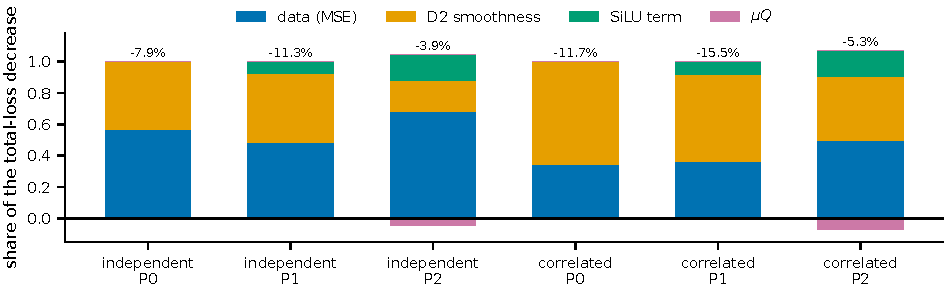
\includegraphics[width=\linewidth]{figS1_lossdecomp.pdf}
  % CAPTION-DRAFT: review (numbers from paper2/figures/figS1_lossdecomp.json)
  \caption{Post hoc loss decomposition (synthetic, early$\to$polished): share of the total-loss decrease from each term, pooled over the 8 seeds of each cell. independent P0: data 0.57, D2 0.43 (median total change -7.9\%); independent P1: data 0.49, D2 0.44 (median total change -11.3\%); independent P2: data 0.68, D2 0.20 (median total change -3.9\%); correlated P0: data 0.35, D2 0.65 (median total change -11.7\%); correlated P1: data 0.37, D2 0.55 (median total change -15.5\%); correlated P2: data 0.50, D2 0.40 (median total change -5.3\%).}
  \label{fig:S1}
\end{figure}


\begin{figure}[h]
  \centering
  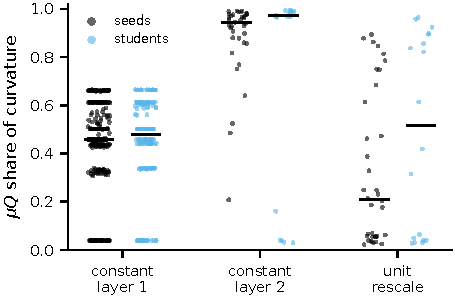
\includegraphics[width=0.5\linewidth]{figS2_gaugecheck.pdf}
  % CAPTION-DRAFT: review (numbers from paper2/figures/figS2_gaugecheck.json)
  \caption{Post hoc gauge check at the $\mu = 10^{-4}$ certified minima: share of the curvature along each least-squares gauge direction contributed by $\mu Q$. Medians: constant shift in layer 1, real-data seeds 0.46 ($n = 288$); constant shift in layer 1, students (trained on a frozen teacher) 0.48 ($n = 144$); constant shift in layer 2, real-data seeds 0.94 ($n = 36$); constant shift in layer 2, students 0.97 ($n = 18$); unit rescaling, real-data seeds 0.21 ($n = 36$); unit rescaling, students 0.52 ($n = 18$).}
  \label{fig:S2}
\end{figure}


\begin{figure}[h]
  \centering
  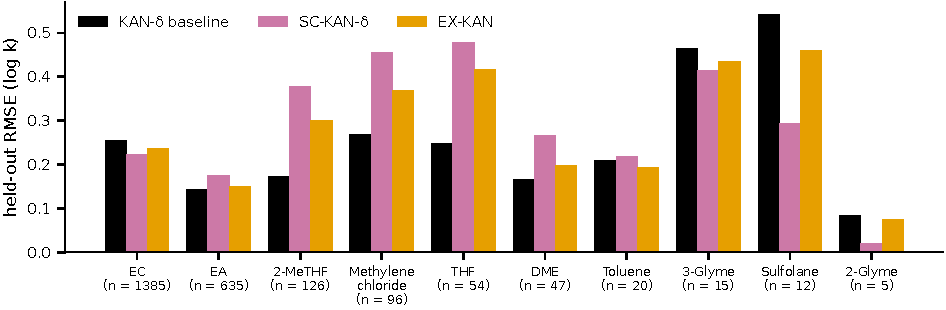
\includegraphics[width=\linewidth]{figS3_loco.pdf}
  % CAPTION-DRAFT: review (numbers from paper2/figures/figS3_loco.json)
  \caption{Leave-one-co-solvent-out RMSE per fold (5-seed ensembles, early state) for the KAN-$\delta$ baseline, SC-KAN-$\delta$ and EX-KAN. Unweighted means: KAN-$\delta$ baseline 0.2554; SC-KAN-$\delta$ 0.2923; EX-KAN 0.2834. The EA fold uses the fold A rows.}
  \label{fig:S3}
\end{figure}

\else % commit hashes replaced by neutral labels (commitmap.json is not part of the submission)
  % GENERATED by build_tex.py (anonymous: commit hashes replaced by labels, see commitmap.json)
\section{All pre-registered predictions}\label{app:prereg}

Generated by \texttt{F-01} from the committed verdict sections; the cell text is the committed wording. Commits are given as pre-registration $\to$ results (in the anonymous version, as neutral labels S-NN). Thresholds are part of each prediction's wording.

\subsection{Synthetic study (\texttt{F-02})}

{\footnotesize\setlength{\tabcolsep}{3pt}
\begin{longtable}{R{0.05\linewidth} R{0.29\linewidth} R{0.36\linewidth} R{0.09\linewidth} R{0.11\linewidth}}
\toprule
ID & Prediction (threshold) & Result & Verdict & Commits \\
\midrule
\endhead
X1 & runaway ($\geq$ 10) in correlated P0 and P1; $\leq$ 3 in the three independent cells and correlated P2 & Correlated P0 $\times$65.7 and P1 $\times$32.1, and P2 $\times$1.00, as predicted. \textbf{But independent P0 $\times$12.5 and P1 $\times$7.9 exceed 3} (independent P2 $\times$1.09) & \textbf{failed} & S-35$\to$\allowbreak S-36 \\
X2 & certified $\leq$ 2/8 in correlated P0 and P1; $\geq$ 6/8 elsewhere & correlated P0 0/8, P1 0/8; independent 6/8, 6/8, 8/8; correlated P2 8/8 & \textbf{held} & S-35$\to$\allowbreak S-36 \\
X3 & cancellation in correlated P0 and P1 each $\geq$ 2 $\times$ correlated P2 & P0 3.29 and P1 2.32, against 2 $\times$ 1.99 = 3.98 & \textbf{failed} & S-35$\to$\allowbreak S-36 \\
X4 & off-manifold ratio $\geq$ 3 in correlated P0 and P1, $\leq$ 1.5 in P2 & P0 1.22, P1 \textbf{0.77}; P2 0.78 (the P2 part held) & \textbf{failed} & S-35$\to$\allowbreak S-36 \\
X5 & Spearman(cancellation, off-manifold RMSE) $\geq$ 0.6 over the 24 correlated models & $\rho$ = +0.177, p = 0.407 & \textbf{failed} & S-35$\to$\allowbreak S-36 \\
X6 & unit match $\geq$ 0.85 in the independent cells and correlated P2; < 0.7 in correlated P0 and P1 & The first part held: 1.000 in all four no-runaway-predicted cells. \textbf{The second part failed: correlated P0 0.774 and P1 0.883 are not < 0.7} & \textbf{failed} & S-35$\to$\allowbreak S-36 \\
\bottomrule
\end{longtable}}
\subsection{Real-data case study (\texttt{F-03})}

Rows are as committed in the case-study summary (one row may cover several predictions, e.g.\ F2--F5). The rank intervention's verdicts are given per arm in the result column.

{\footnotesize\setlength{\tabcolsep}{3pt}
\begin{longtable}{R{0.14\linewidth} R{0.26\linewidth} R{0.29\linewidth} R{0.10\linewidth} R{0.11\linewidth}}
\toprule
Study & Prediction (threshold) & Result & Verdict & Commits \\
\midrule
\endhead
Gauge study (\texttt{gauge\_\allowbreak{}F-04}) & \textbf{Control 1}: teacher edges recovered, median dense corr $\geq$ 0.8 & 0.301 (sanity: h corr 0.913 < 0.95) & \textbf{failed} & S-02$\to$\allowbreak{}S-03 \\
Gauge study (\texttt{gauge\_\allowbreak{}F-04}) & P1: gauge fixing removes $\geq$ 50\% of edge variance & not run & inconclusive (gated by Control 1) & S-02$\to$\allowbreak{}S-03 \\
Gauge study (\texttt{gauge\_\allowbreak{}F-04}) & P2: sparse $\geq$ 2$\times$ dense, DEC region highest & not run & inconclusive (gated) & S-02$\to$\allowbreak{}S-03 \\
Gauge study (\texttt{gauge\_\allowbreak{}F-04}) & P3: (e) < (d) < (c) < (a) & not run & inconclusive (gated) & S-02$\to$\allowbreak{}S-03 \\
Gauge study (\texttt{gauge\_\allowbreak{}F-04}) & P4: every seed has a unit with |corr| < 0.8 & not run & inconclusive (gated) & S-02$\to$\allowbreak{}S-03 \\
Gauge study (\texttt{gauge\_\allowbreak{}F-04}) & P5: KAN-full edge variance > KAN-delta & not run & inconclusive (gated) & S-02$\to$\allowbreak{}S-03 \\
Gauge study (\texttt{gauge\_\allowbreak{}F-04}) & P6: seed spread flags errors & Spearman +0.169 (A) / +0.213 (B); fold B RMSE at 80\% coverage 0.153 vs random 0.137 & \textbf{failed} & S-02$\to$\allowbreak{}S-04 \\
Control 2 (\texttt{control2\_\allowbreak{}F-04}) & C1: (I,C) edges $\geq$ 0.9 and units $\geq$ 0.9 & prediction corr 0.947 < 0.99 & inconclusive (gate failed) & S-05$\to$\allowbreak{}S-06 \\
Control 2 (\texttt{control2\_\allowbreak{}F-04}) & C2: (R,C) invT, molal $\geq$ 0.9; co-solvent < 0.7 & prediction corr 0.969 < 0.99 & inconclusive (gate failed) & S-05$\to$\allowbreak{}S-06 \\
Control 2 (\texttt{control2\_\allowbreak{}F-04}) & C3: 107 epochs gives prediction corr < 0.95 & 0.858 (I,S), 0.919 (R,S) & \textbf{held} & S-05$\to$\allowbreak{}S-06 \\
Control 3 (\texttt{control3\_\allowbreak{}F-04}) & C1': (I) passes the gate, edges $\geq$ 0.9, units $\geq$ 0.9 & (I) RMSE/std 0.128 > 0.05; unit match 0.648 & \textbf{failed} & S-07$\to$\allowbreak{}S-08 \\
Control 3 (\texttt{control3\_\allowbreak{}F-04}) & C2': (R) edges $\leq$ (I) edges $-$ 0.10 & (R) edges 0.852, units 0.659 & inconclusive ((I) failed the gate) & S-07$\to$\allowbreak{}S-08 \\
Control 3 (\texttt{control3\_\allowbreak{}F-04}) & C4: every continuous input $\geq$ 0.9 in (I) & -- & inconclusive ((I) failed the gate) & S-07$\to$\allowbreak{}S-08 \\
Fiber (\texttt{fiber\_\allowbreak{}F-04}) & F1: $\geq$ 50\% of seed pairs on-fiber & 0/190 (closest d = 0.146) & \textbf{failed} & S-09$\to$\allowbreak{}S-10 \\
Fiber (\texttt{fiber\_\allowbreak{}F-04}) & F2--F5 & not run & inconclusive (no on-fiber pairs) & S-09$\to$\allowbreak{}S-10 \\
Fiber 2 (\texttt{fiber2\_\allowbreak{}F-04}) & G1: $\geq$ 4/6 seeds and $\geq$ 10/20 students certify convergence & 0/6, 0/20 (all at the 20,000-iteration cap) & \textbf{failed} & S-11$\to$\allowbreak{}S-12 \\
Fiber 2 (\texttt{fiber2\_\allowbreak{}F-04}) & G2--G5 & not run & inconclusive (no converged model) & S-11$\to$\allowbreak{}S-12 \\
Support (\texttt{support\_\allowbreak{}F-04}) & H1: dim(N) $\geq$ 5 & dim(N) = 36 of 72 & \textbf{held} & S-13$\to$\allowbreak{}S-14 \\
Support (\texttt{support\_\allowbreak{}F-04}) & H2: $\geq$ 50\% of N is REDISTRIBUTION within the correlated group & 18/36 & \textbf{held, exactly at threshold} & S-13$\to$\allowbreak{}S-14 \\
Support (\texttt{support\_\allowbreak{}F-04}) & H3: set A fraction in N $\geq$ 0.5 and $\geq$ 3$\times$ random & median 0.942 (random 0.5) & inconclusive (untestable: 3 $\times$ 0.5 > 1) & S-13$\to$\allowbreak{}S-14 \\
Support (\texttt{support\_\allowbreak{}F-04}) & H4: set B (capped), same criterion & median 0.949 & inconclusive (untestable) & S-13$\to$\allowbreak{}S-14 \\
Support (\texttt{support\_\allowbreak{}F-04}) & H5: flattest Hessian directions overlap N $\geq$ 0.5 & median 0.885; median layer-1 block share only 0.08 & \textbf{held}, with caveat (see \texttt{support\_\allowbreak{}F-04}) & S-13$\to$\allowbreak{}S-14 \\
Support (\texttt{support\_\allowbreak{}F-04}) & H6: fraction in N rises from control-3 to capped state, $\geq$ 15/20 & 20/20 (0.713 $\to$\allowbreak{} 0.949) & \textbf{held} & S-13$\to$\allowbreak{}S-14 \\
Rule (\texttt{rule\_\allowbreak{}F-04}) & I1--I5 (gate) & 0 columns removed; gate stopped & inconclusive & S-16$\to$\allowbreak S-17 \\
Rank (\texttt{rank\_\allowbreak{}F-04}) & I1: median max|grad| $\leq$ 0.1 $\times$ baseline & arm G: \textbf{failed} (4.00$\times$); arm F: \textbf{failed} (29.1$\times$) & see result & S-18$\to$\allowbreak S-19 \\
Rank (\texttt{rank\_\allowbreak{}F-04}) & I2: median d\_AB $\leq$ 0.5 $\times$ baseline & arm G: \textbf{failed} (0.945$\times$); arm F: \textbf{failed} (0.808$\times$) & see result & S-18$\to$\allowbreak S-19 \\
Rank (\texttt{rank\_\allowbreak{}F-04}) & I3 (sanity): median loss $\leq$ 1.10 $\times$ baseline & arm G: passed (1.004$\times$); arm F: passed, narrowly (1.099$\times$) & see result & S-18$\to$\allowbreak S-19 \\
Rank (\texttt{rank\_\allowbreak{}F-04}) & I4: fold A RMSE $\leq$ 0.150 (KAN-delta 0.1420) & arm G: \textbf{held}, narrowly (0.1499); arm F: \textbf{failed} (0.1587) & see result & S-18$\to$\allowbreak S-19 \\
Rank (\texttt{rank\_\allowbreak{}F-04}) & I5: edge corr on 1000/T and molality $\geq$ baseline + 0.1 (baseline 0.102) & arm G: \textbf{held} (0.927); arm F: \textbf{held} (0.338) & see result & S-18$\to$\allowbreak S-19 \\
Rank (\texttt{rank\_\allowbreak{}F-04}) & I6: arm F's improvement $\geq$ arm G's in both I1 and I2 & arm G: \textbf{failed} (max|grad| 29.1$\times$ vs 4.00$\times$; d\_AB does favour F, 0.808 vs 0.945) & see result & S-18$\to$\allowbreak S-19 \\
\texttt{trust\_\allowbreak{}F-04} & T1 / T2: trust-krylov certifies $\geq$ 4/6 seeds / $\geq$ 2/3 students & 0/6, 0/3. All 9 stopped on scipy's "bad approximation" after 1--62 iterations; the Hessian was accurate to $\leq$ 2e-7 & \textbf{failed} & S-20$\to$\allowbreak S-21 \\
\texttt{trust\_\allowbreak{}F-04} & T3--T5 & nothing converged & inconclusive & S-20$\to$\allowbreak S-21 \\
\texttt{stage2\_\allowbreak{}F-04} & U1: trust-exact (exact Hessian, 500 iterations) certifies $\geq$ 4/6 seeds & 0/6. All 9 hit the iteration cap & \textbf{failed} & S-22$\to$\allowbreak S-26 \\
\texttt{stage2\_\allowbreak{}F-04} & U2: with L2 $\lambda$ = 1e-5, $\geq$ 4/6 seeds and $\geq$ 2/3 students & 1/6 seeds, 0/3 students & \textbf{failed} & S-22$\to$\allowbreak S-26 \\
\texttt{stage2\_\allowbreak{}F-04} & U3: more converge at 1e-5 than at 1e-6 & 1 vs 0 & \textbf{held} & S-22$\to$\allowbreak S-26 \\
\texttt{stage2\_\allowbreak{}F-04} & U4: converged L2 models' loss without L2 $\leq$ 1.05 $\times$ capped & 1.2545 & \textbf{failed} & S-22$\to$\allowbreak S-26 \\
\texttt{stage2\_\allowbreak{}F-04} & U5: converged seeds' disagreement $\leq$ 0.5 $\times$ capped & only 1 converged & inconclusive & S-22$\to$\allowbreak S-26 \\
\texttt{close\_\allowbreak{}F-04} & V1: at some $\mu$, $\geq$ 4/6 seeds and $\geq$ 2/3 students converge (stage2 criterion) & 0 certified at every $\mu$ & \textbf{failed} & S-29$\to$\allowbreak{}S-30 \\
\texttt{close\_\allowbreak{}F-04} & V2: converged seeds' data term $\leq$ 1.05 $\times$ stage2 A & nothing certified at the selected $\mu$ = 1e-6 & inconclusive & S-29$\to$\allowbreak{}S-30 \\
\texttt{close\_\allowbreak{}F-04} & V3: $\|\theta\|^{2}$ $\leq$ 10 $\times$ start & same & inconclusive & S-29$\to$\allowbreak{}S-30 \\
\texttt{close\_\allowbreak{}F-04} & V4: seed disagreement halved & same & inconclusive & S-29$\to$\allowbreak{}S-30 \\
\texttt{close\_\allowbreak{}F-04} & V5: students' unit match $\geq$ 0.8 & same & inconclusive & S-29$\to$\allowbreak{}S-30 \\
\texttt{close\_\allowbreak{}F-04} & V6: fold A RMSE $\leq$ 0.150 & 1.0262, bias +0.9028 & \textbf{failed} & S-29$\to$\allowbreak{}S-30 \\
\texttt{certify\_\allowbreak{}F-04} & W1: at $\mu$ = 1e-4, $\geq$ 5/6 seeds certified (second-order criterion, F-a) & 6/6; all 17 candidates certified & \textbf{held} & S-31$\to$\allowbreak{}S-32 \\
\texttt{certify\_\allowbreak{}F-04} & W2: certified seeds' median d\_AB $\leq$ 0.5 $\times$ capped & 0.0771 vs capped 0.1041 ($-$26\%) & \textbf{failed} & S-31$\to$\allowbreak{}S-32 \\
\texttt{certify\_\allowbreak{}F-04} & W3: certified students' unit match $\geq$ 0.8 (vs the original teacher) & 0.624 & \textbf{failed} & S-31$\to$\allowbreak{}S-32 \\
\texttt{certify\_\allowbreak{}F-04} & W4: $\mu$ = 1e-4 fold A RMSE $\leq$ 0.150 & 0.3345 & \textbf{failed} & S-31$\to$\allowbreak{}S-32 \\
\texttt{certify\_\allowbreak{}F-04} & W5: $\mu$ = 1e-4 fold A RMSE $\leq$ 0.5131 & 0.3345 & \textbf{held} & S-31$\to$\allowbreak{}S-32 \\
\texttt{certify\_\allowbreak{}F-04} & W6: Spearman(cross-edge ratio, held-out RMSE) $\geq$ 0.6 & $\rho$ = +0.345, p = 0.328 (weak test) & \textbf{failed} & S-31$\to$\allowbreak{}S-32 \\
\bottomrule
\end{longtable}}
\noindent Committed tally of the case study:

{\footnotesize\setlength{\tabcolsep}{3pt}
\begin{longtable}{R{0.55\linewidth} r r r}
\toprule
Study & Held & Failed & Inconclusive \\
\midrule
\endhead
First table (Control 1, P1--P6, C1--C3, C1'/C2'/C4, F1--F5, G1--G5, H1--H6) & 5 & 5 & 19 \\
Rule (I1--I5) & 0 & 0 & 5 \\
Rank (I1, I2, I4, I5 per arm, I6) & 3 & 6 & 0 \\
Trust (T1--T5) & 0 & 2 & 3 \\
Stage 2 (U1--U5) & 1 & 3 & 1 \\
Close (V1--V6) & 0 & 2 & 4 \\
Certify (W1--W6) & 2 & 4 & 0 \\
\textbf{Total} & \textbf{11} & \textbf{22} & \textbf{32} \\
\bottomrule
\end{longtable}}
\subsection{Shared-curve KAN (\texttt{F-05})}

Run after the case-study close-out; not part of the 65 predictions above.

{\footnotesize\setlength{\tabcolsep}{3pt}
\begin{longtable}{R{0.05\linewidth} R{0.26\linewidth} R{0.39\linewidth} R{0.09\linewidth} R{0.11\linewidth}}
\toprule
ID & Prediction (threshold) & Result & Verdict & Commits \\
\midrule
\endhead
S1 & SC LOCO RMSE $\leq$ 1.05 $\times$ baseline & unweighted mean SC 0.2923 vs base 0.2554 (ratio 1.145; threshold 0.2681). Also reported: row-weighted 0.2478 / 0.2297 (1.079); folds $\geq$ 20 rows 0.3138 / 0.2093 (1.499) & failed & S-38$\to$\allowbreak S-40 \\
S2 & SC fold A RMSE $\leq$ 0.160 & SC 0.1757 (base 0.1420) & failed & S-38$\to$\allowbreak S-40 \\
S3 & SC median d\_AB $\leq$ 0.5 $\times$ baseline & SC 0.1865 vs base 0.1120 (threshold 0.0560): SC seeds agree \emph{less} than baseline seeds & failed & S-38$\to$\allowbreak S-40 \\
S4 & curve corr $\geq$ 0.90 for $\geq$ 6 of 8 inputs & 3 of 8 (M\_co 0.959, mix\_lneta 0.970, invT 0.986); lowest x\_co 0.596; others 0.871--0.891 & failed & S-38$\to$\allowbreak S-40 \\
S5 & $\geq$ 8/10 SC fold A models certified & SC 10/10 (max|grad| $\leq$ 7e-10, 0 near-null eigenvalues); baseline 0/10 (all hit the 500-iteration cap) & held & S-38$\to$\allowbreak S-40 \\
S6 & median $\beta$-norm polished/early $\leq$ 3 (calibrated) & median 1.337 (range 0.652--2.356); $\|\theta\|^{2}$ $\times$4.59 (base $\times$67.9, range 30.6--281) & held & S-38$\to$\allowbreak S-40 \\
S7 & SC polished/early fold A RMSE $\leq$ 1.5 & SC 1.920 (0.1757 $\to$\allowbreak{} 0.3373); baseline 5.736 (0.1420 $\to$\allowbreak{} 0.8147) & failed & S-38$\to$\allowbreak S-40 \\
S8 & d log k/d(1000/T) < 0 on $\geq$ 95\% rows in $\geq$ 8/10 seeds & 10/10 (median share 1.000; 1424 rows, 10 excluded per D4) & held & S-38$\to$\allowbreak S-40 \\
S9 & Spearman(1000/T, |slope|) > 0 in $\geq$ 8/10 seeds & 10/10 (median +0.661, range +0.406 to +0.885) & held & S-38$\to$\allowbreak S-40 \\
S10 & d log k/d(ln $\eta$\_mix) < 0 on $\geq$ 90\% rows in $\geq$ 8/10 seeds & 7/10 (median share 0.967; s0 0.892, s2 0.892, s8 0.826) & failed & S-38$\to$\allowbreak S-40 \\
\bottomrule
\end{longtable}}
\subsection{Two-anchor excess model (\texttt{F-06})}

Run after the case-study close-out; not part of the 65 predictions above.

{\footnotesize\setlength{\tabcolsep}{3pt}
\begin{longtable}{R{0.05\linewidth} R{0.26\linewidth} R{0.39\linewidth} R{0.09\linewidth} R{0.11\linewidth}}
\toprule
ID & Prediction (threshold) & Result & Verdict & Commits \\
\midrule
\endhead
E1 & EX LOCO $\leq$ 0.95 $\times$ KAN-delta & unweighted mean EX 0.2834 vs threshold 0.2426 (base 0.2554; ratio 1.110). Row-weighted 0.2363 / 0.2297 (1.029); folds $\geq$ 20 rows 0.2662 / 0.2093 (1.272). EX is better on EC (0.237 vs 0.256), Sulfolane, 3-Glyme, 2-Glyme and Toluene, and worse on 2-MeTHF, THF, Methylene chloride, DME and EA & failed & S-41$\to$\allowbreak S-43 \\
E2 & EX fold A $\leq$ 0.142 & EX 0.1502 (base this run 0.1420) & failed & S-41$\to$\allowbreak S-43 \\
E3 & s agrees across seeds (separable co-solvents, Amendment 1) & median pairwise corr +0.987 over EA, EC, Methylene chloride: a weak test with 3 values per seed, and Methylene chloride is marginal. Seed SD of s: EA 0.063 (0.39 $\times$ the spread across co-solvents, 0.159), EC 0.091 (0.57 $\times$), Methylene chloride 0.067 (0.42 $\times$). Secondary ($\leq$ 2 rule, 7 co-solvents): +0.869 & held & S-41$\to$\allowbreak S-43 \\
E4 & mean s(low $\varepsilon$) < mean s(EC, Sulfolane) in $\geq$ 8/10 seeds & 0/10: the ordering is reversed in every seed. Per high-$\varepsilon$ co-solvent: vs EC alone 0/10 (EC median s +0.104), vs Sulfolane alone 0/10 (median $-$0.124). The low-$\varepsilon$ mean is +0.19 to +0.49 per seed. Sulfolane does not drive the failure on its own: EC alone fails in every seed too & failed & S-41$\to$\allowbreak S-43 \\
E5 & median seed-SD flagged $\geq$ 2 $\times$ separable (Amendment 1) & 0.091 vs 0.067, ratio 1.37. Secondary ($\leq$ 2 rule): 0.222 vs 0.069, ratio 3.22, no verdict; the secondary is driven by 3-Glyme (SD 0.478, M\_co extrapolated) and 2-Glyme (0.222) & failed & S-41$\to$\allowbreak S-43 \\
\bottomrule
\end{longtable}}% GENERATED by build_tex.py (anonymous: commit hashes replaced by labels, see commitmap.json)
\section{Post-hoc analyses}\label{app:posthoc}

Every analysis below was defined after seeing results. Each is labelled \textbf{post hoc} in its own files, changes no pre-registered verdict, and is reported as exploratory. The description is the subject line of the commit that added the analysis.

{\footnotesize\setlength{\tabcolsep}{3pt}\begin{longtable}{R{0.28\linewidth} R{0.52\linewidth} R{0.10\linewidth}}
\toprule
Analysis & Commit subject (as committed) & Commit \\
\midrule
\endhead
\textbf{Post hoc.} Anatomy of the real-data runaway \newline \footnotesize{\texttt{F-07, F-08, F-09}} & Plan for descriptive runaway anatomy (before F-08 exists) & S-27 \\
 & Anatomy (descriptive): Q1, Q2 not as expected, Q3 as expected; RBF growth is in the penalty null space & S-28 \\
\textbf{Post hoc.} Gauge check and regularised teacher (exploratory) \newline \footnotesize{\texttt{F-10, F-11, F-12}} & gaugecheck (POST-HOC, exploratory): penalty fixes gauge position by slope balance; students match the regularised teacher & S-33 \\
\textbf{Post hoc.} Anatomy of the synthetic runaway \newline \footnotesize{\texttt{F-13, F-14}} & paper2 anatomy\_synth (POST-HOC, descriptive): synthetic runaway lives mainly in layer-2 output-edge cancellation, unsaturated; no verdicts change & S-37 \\
\textbf{Post hoc.} Loss decomposition along the runaway \newline \footnotesize{\texttt{F-15, F-16}} & paper2 lossdecomp (POST-HOC, descriptive): synthetic runaway loss decrease shared, D2 penalty median 0.61 vs data 0.37; 12/20 runaway models overfit; real-data reference recomputed & S-44 \\
\textbf{Post hoc.} Descriptive checks (hidden-unit correlation, tilt affinity, references) \newline \footnotesize{\texttt{F-17, F-18, F-19}} & paper2/checks: plan for descriptive checks (F4 hidden-unit correlation, F2 tilt affinity, A1 commit and data citation) before F-20 exists & S-46 \\
 & paper2/checks (POST-HOC, descriptive): hidden-unit correlation marks the runaway (independent cells 0.70 vs 0.05) but is not sufficient; RBF tilt affine to 2\% centrally, 13\% at the ends; A1 commit S-01; CALiSol-23 citation not in competition material & S-47 \\
\textbf{Post hoc.} Regularised teacher (weights pinned) & Pin gaugecheck regularised-teacher weights in a seventh archive; append to weights manifest & S-34 \\
\bottomrule
\end{longtable}}% GENERATED by build_tex.py (anonymous: commit hashes replaced by labels, see commitmap.json)
\section{Reproducibility map}\label{app:repro}

Generated from \texttt{F-42}. Every figure is rebuilt by its script from committed results; each figure's sidecar JSON lists the data files (path, commit, SHA-256), any archived weights (SHA-256, archive) and every plotted number. \REPOSTATEMENT

{\footnotesize\setlength{\tabcolsep}{3pt}
\begin{longtable}{R{0.15\linewidth} R{0.13\linewidth} R{0.42\linewidth} R{0.19\linewidth}}
\toprule
Figure & Script & Data files (commit) & Archived weights \\
\midrule
\endhead
Figure~\ref{fig:mechanism} \figname{fig1\_mechanism} & \texttt{F-43} & none (computed from committed code: F-02, F-44) & --- \\
Figure~\ref{fig:synthetic} \figname{fig2\_synthetic} & \texttt{F-45} & \texttt{F-46} (S-36) & --- \\
Figure~\ref{fig:where} \figname{fig3\_where} & \texttt{F-47} & \texttt{F-48} (S-88); \texttt{F-49} (S-37); \texttt{F-50} (S-48) & 18 files, archives W-01, W-02, W-03 \\
Figure~\ref{fig:applicability} \figname{fig4\_applicability} & \texttt{F-51} & \texttt{F-34} (S-90); \texttt{F-48} (S-88) & 15 files, archives W-04, W-05, W-06 \\
Figure~\ref{fig:paths} \figname{fig5\_paths} & \texttt{F-52} & \texttt{F-53} (S-59) & --- \\
Figure~\ref{fig:corrdose} \figname{fig6\_correlation\_dose} & \texttt{F-54} & \texttt{F-55} (S-64) & --- \\
Figure~\ref{fig:bspline} \figname{fig7\_bspline} & \texttt{F-56} & \texttt{F-46} (S-36); \texttt{F-57} (S-81); \texttt{F-30} (S-86) & --- \\
Figure~\ref{fig:dose} \figname{fig8\_dose\_response} & \texttt{F-58} & \texttt{F-59} (S-26); \texttt{F-60} (S-30); \texttt{F-61} (S-32) & --- \\
Figure~\ref{fig:uniqueness} \figname{fig9\_uniqueness} & \texttt{F-62} & \texttt{F-63} (S-41); \texttt{F-61} (S-32); \texttt{F-48} (S-88) & 40 files, archives W-05 \\
Figure~\ref{fig:S1} \figname{figS1\_lossdecomp} & \texttt{F-64} & \texttt{F-65} (S-46) & --- \\
Figure~\ref{fig:S2} \figname{figS2\_gaugecheck} & \texttt{F-64} & \texttt{F-66} (S-33) & --- \\
Figure~\ref{fig:S3} \figname{figS3\_loco} & \texttt{F-64} & \texttt{F-63} (S-41); \texttt{F-67} (S-45) & --- \\
\bottomrule
\end{longtable}}
\noindent Tables in the main text (no script; values typed in the draft):

{\footnotesize\setlength{\tabcolsep}{3pt}
\begin{longtable}{R{0.14\linewidth} R{0.14\linewidth} R{0.45\linewidth} R{0.16\linewidth}}
\toprule
Table & Source & Data files & Commits \\
\midrule
\endhead
Table~\ref{tab:synthetic} & typed in the draft from & \texttt{F-46}, \texttt{F-68} & S-36 \\
Table~\ref{tab:dose} & typed in the draft from & \texttt{F-60}, \texttt{F-61}, \texttt{F-59} & S-30, S-32, S-26 \\
Table~\ref{tab:alternatives} & typed in the draft from & \texttt{F-63}, \texttt{F-67}, \texttt{F-69} & S-41, S-45, S-49 \\
\bottomrule
\end{longtable}}
\noindent Panels evaluated post hoc from archived weights (from \texttt{F-70}):

\begin{itemize}
  \item \textbf{fig3a, real data:} the split of the parameter change into affine and curved RBF parts per layer, for 107 epochs $\to$\allowbreak{} fiber2 capped $\to$\allowbreak{} stage2 Part A.
  \item \texttt{F-59} stores only per-block norms, without an affine/curved split and without the 107 $\to$\allowbreak{} capped change.
  \item \textbf{fig9b, polished fold A d\_AB} for SC-KAN-$\delta$ and the baseline (marked *).
  \item arch/sc committed d\_AB only at the early state.
  \item \textbf{fig4a, b, fold A per-row error change} (early-stopped -> mu = $10^{-6}$ and mu = $10^{-4}$ ensembles).
  \item F-71 stores only the per-row Spearman correlations and medians; the per-row values are re-evaluated with the
\end{itemize}% GENERATED by build_tex.py (anonymous: commit hashes replaced by labels, see commitmap.json)
\section{Research process}\label{app:process}

% DRAFT-TEXT: review (new prose, not in the source draft; it states only the protocol followed, no results). First and last paragraphs: author-supplied wording (2026-10-05)
\paragraph{Pre-registration.} Every study committed a pre-registration file (predictions, thresholds, interpretation rules) before the script that tested it existed. Verdicts were appended below the committed text; the pre-registered text was never edited, and corrections to reported numbers were made in separate, labelled commits.
\paragraph{Amendments.} A change to a design after its pre-registration was committed as a dated amendment section before any affected model was trained, with its reason; the original text was kept. Choices forced by the code or data at run time were logged as numbered discrepancies at the top of each output log.
\paragraph{Files win.} Instructions to the agent stated that committed files take precedence over any number or description in a prompt; discrepancies between a brief and the files were flagged rather than resolved silently.
\paragraph{Data and weights.} Model weights were never committed: they were archived outside the repository with a manifest of SHA-256 hashes and producing commits, and every later analysis verified the hashes and held its inputs in memory. Post-hoc analyses were labelled as such in their files and changed no verdict.
\paragraph{AI assistance.} Code, runs and logs were produced by an AI coding agent working under this protocol. Study designs, briefs and the manuscript were developed with an AI assistant. The author set the research questions, reviewed and approved every brief and amendment, decided each next stage, and takes responsibility for all content. Crashes were recorded in the logs and fixed in separate commits labelled as implementation-only.

\noindent Pre-registrations, amendments and crash records (from the commit history):

{\footnotesize\setlength{\tabcolsep}{3pt}
\begin{longtable}{R{0.08\linewidth} R{0.10\linewidth} R{0.14\linewidth} R{0.58\linewidth}}
\toprule
Commit & Date & Kind & Commit subject \\
\midrule
\endhead
S-02 & 2026-09-23 & pre-registration & Pre-register KAN identifiability study (before any experiment) \\
S-05 & 2026-09-23 & pre-registration & Pre-register corrected 2x2 control (before writing or running it) \\
S-07 & 2026-09-23 & pre-registration & Pre-register control 3: reachable teacher (before writing code) \\
S-09 & 2026-09-29 & pre-registration & Pre-register fiber completeness test (before writing or running F-41) \\
S-11 & 2026-09-29 & pre-registration & Pre-register fiber2: certified convergence + teacher-known fiber analysis (before writing code) \\
S-13 & 2026-09-29 & pre-registration & Pre-register support study: near-null space, where models differ, Hessian (before F-42 exists) \\
S-15 & 2026-09-29 & pre-registration & Close-out: electrolyte case study summary (all pre-registered predictions) \\
S-16 & 2026-09-29 & pre-registration & Pre-register basis-size rule intervention (before F-43 exists) \\
S-18 & 2026-09-29 & pre-registration & Pre-register rank-constrained layer-1 intervention (before F-44 exists) \\
S-20 & 2026-09-30 & pre-registration & Pre-register trust-region Newton polishing, stage 1 (before F-45 exists) \\
S-22 & 2026-09-30 & pre-registration & Pre-register stage 2: trust-exact check, runaway diagnostic, coercivity (before F-46 exists) \\
S-23 & 2026-09-30 & crash record / fix & F-46 as first run (crashed with AttributeError in callback) \\
S-24 & 2026-09-30 & crash record / fix & stage2: fix AttributeError (implementation only, post-prereg) \\
S-25 & 2026-10-02 & crash record / fix & stage2: hold verified inputs in memory (implementation only, post-prereg) \\
S-29 & 2026-10-02 & pre-registration & Pre-register targeted null-space penalty intervention (before F-47 exists) \\
S-31 & 2026-10-03 & pre-registration & Pre-register second-order certification and regularised fold A accuracy (before F-48 exists) \\
S-35 & 2026-10-03 & pre-registration & paper2: pre-register synthetic 2x3 runaway test (before F-49 exists) \\
S-38 & 2026-10-03 & pre-registration & arch: pre-register SC-KAN-$\delta$ (shared-curve KAN-$\delta$) before any script exists; decisions C (centring), mu null-space term, tanh salt embedding, full beta term \\
S-39 & 2026-10-03 & crash record / fix & arch sc\_run: fix log() call (crash record 1, after the first fold A polish); resume from cache \\
S-41 & 2026-10-04 & pre-registration & arch: pre-register EX-KAN (two-anchor excess model) before any script exists; decision B (x\_co-independent g, [7,6,1]), full set for E3-E5, E4 mean rule \\
S-42 & 2026-10-04 & amendment & arch ex\_prereg: Amendment 1 (after Step 0, before training): primary separability rule by fixed-composition groups (EA, EC, Methylene chloride separable); committed rule reported as secondary \\
\bottomrule
\end{longtable}}% GENERATED by build_tex.py (anonymous: commit hashes replaced by labels, see commitmap.json)
\section{Supplementary figures}\label{app:supp}


\begin{figure}[htbp]
  \centering
  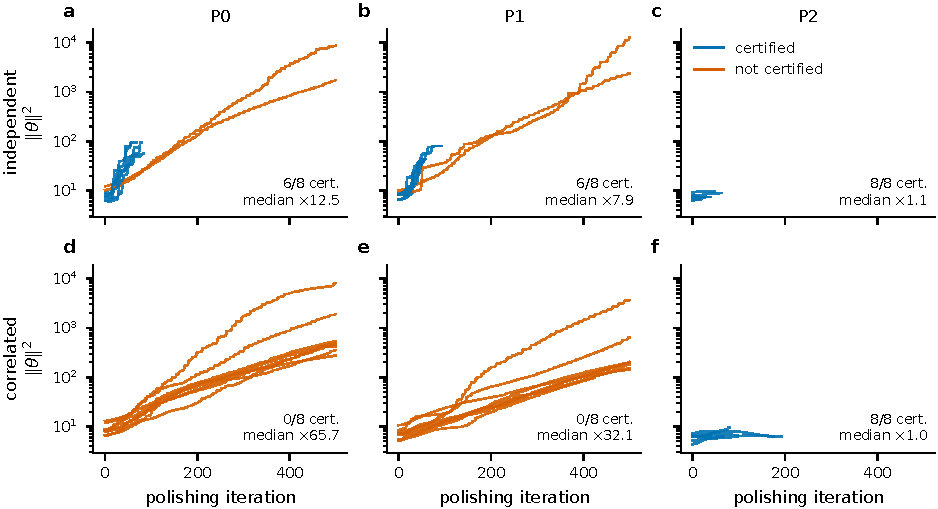
\includegraphics[width=\linewidth]{fig2_synthetic.pdf}
  % CAPTION-DRAFT: review (numbers from paper2/figures/fig2_synthetic.json)
  \caption{Synthetic $2\times3$ study: $\|\theta\|^2$ over exact-Hessian trust-region polishing iterations (log scale), one line per seed, coloured certified (blue) or not certified (vermillion). Rows: independent and correlated inputs; columns: P0, P1, P2. Per panel, certified seeds and median growth (polished over early-stopped): independent P0: 6/8 certified, $\times$12.5; independent P1: 6/8 certified, $\times$7.9; independent P2: 8/8 certified, $\times$1.1; correlated P0: 0/8 certified, $\times$65.7; correlated P1: 0/8 certified, $\times$32.1; correlated P2: 8/8 certified, $\times$1.0.}
  \label{fig:synthetic}
\end{figure}


\begin{figure}[htbp]
  \centering
  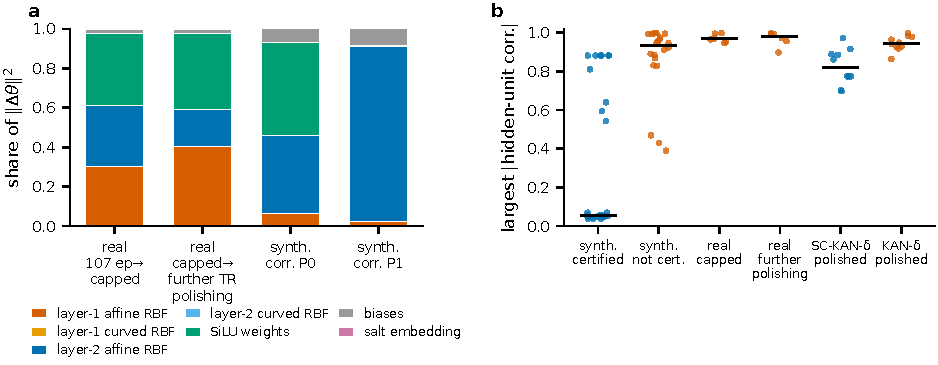
\includegraphics[width=\linewidth]{fig3_where.pdf}
  % CAPTION-DRAFT: review (numbers from paper2/figures/fig3_where.json)
  \caption{Where the runaway lives. \textbf{(a)} Mean share of $\|\Delta\theta\|^2$ by parameter block. Real data, 107 epochs$\to$capped: layer-1 affine RBF 0.30, layer-2 affine RBF 0.31, SiLU weights 0.37; capped$\to$further trust-region polishing: 0.40, 0.19, 0.38; synthetic correlated P0: layer-2 affine RBF 0.39, SiLU weights 0.47; correlated P1: layer-2 affine RBF 0.89. The real-data split was evaluated post hoc from archived weights (Appendix~\ref{app:repro}). \textbf{(b)} Largest absolute correlation between hidden-unit activations on the training rows, median: synthetic, certified 0.054 ($n=28$); synthetic, not certified 0.935 ($n=20$); real, capped 0.968 ($n=6$); real, further polishing 0.983 ($n=6$); SC-KAN-$\delta$ polished 0.818 ($n=10$); KAN-$\delta$ polished 0.946 ($n=10$). Blue: certified; vermillion: not certified or runaway.}
  \label{fig:where}
\end{figure}


\begin{figure}[htbp]
  \centering
  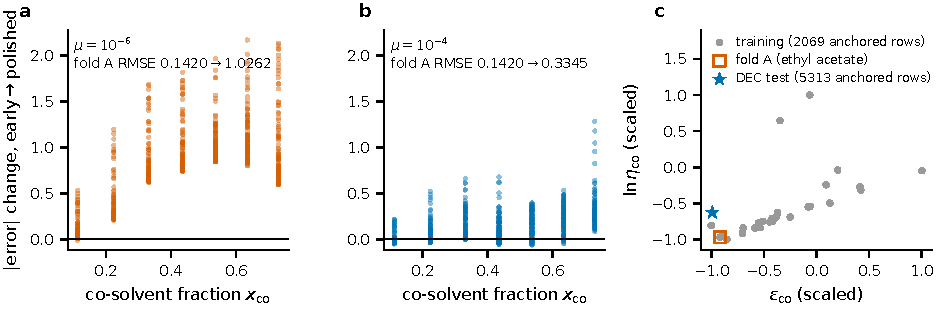
\includegraphics[width=\linewidth]{fig4_applicability.pdf}
  % CAPTION-DRAFT: review (numbers from paper2/figures/fig4_applicability.json)
  \caption{Applicability (descriptive; analysis plan committed before computing). \textbf{(a, b)} Fold A (ethyl acetate held out, 635 rows): change in each row's absolute error from the early-stopped 5-seed ensemble to the polished ensemble, against the co-solvent fraction $x_{\mathrm{co}}$ (7 distinct values); fold A RMSE 0.1420$\to$1.0262 at $\mu = 10^{-6}$ (a) and 0.1420$\to$0.3345 at $\mu = 10^{-4}$ (b). Per-row values are evaluated post hoc from SHA-verified archived weights, with the logged RMSEs reproduced (Appendix~\ref{app:repro}). \textbf{(c)} Co-solvent descriptors $\varepsilon_{\mathrm{co}}$ and $\ln\eta_{\mathrm{co}}$ in the committed min--max scaling: the 2069 anchored training rows (30 distinct points), fold A's co-solvent (off-pattern distance 0.047) and the 5313 anchored DEC test rows (0.334); each held-out set occupies a single point.}
  \label{fig:applicability}
\end{figure}


\begin{figure}[htbp]
  \centering
  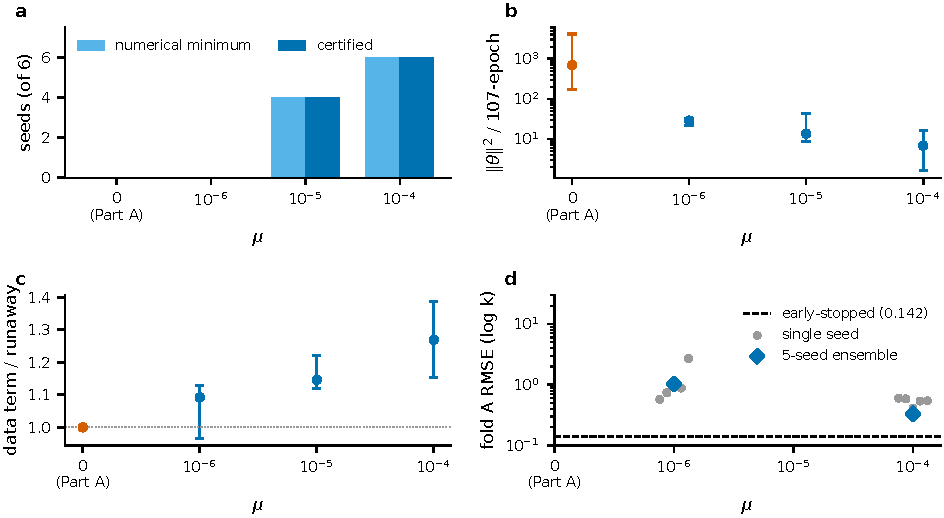
\includegraphics[width=\linewidth]{fig8_dose_response.pdf}
  % CAPTION-DRAFT: review (numbers from paper2/figures/fig8_dose_response.json)
  \caption{Real-data dose-response in the null-space weight $\mu$ (6 KAN-$\delta$ seeds; $\mu = 0$: polished without a null-space penalty). \textbf{(a)} Seeds at a numerical minimum (all of them certified): $\mu = 0$, 0 of 6; $10^{-6}$, 0 of 6; $10^{-5}$, 4 of 6; $10^{-4}$, 6 of 6. \textbf{(b)} $\|\theta\|^2$ relative to the 107-epoch state, median (range): $\mu = 0$, 690 (170--4146); $10^{-6}$, 29 (21--31); $10^{-5}$, 14 (9--43); $10^{-4}$, 7 (2--16). \textbf{(c)} Training data term relative to the runaway, median: $10^{-6}$, 1.092; $10^{-5}$, 1.146; $10^{-4}$, 1.269. \textbf{(d)} Fold A RMSE: early-stopped 0.142 (dashed line); polished 5-seed ensemble 1.026 at $\mu = 10^{-6}$ and 0.334 at $\mu = 10^{-4}$; grey points are single seeds.}
  \label{fig:dose}
\end{figure}


\begin{figure}[h]
  \centering
  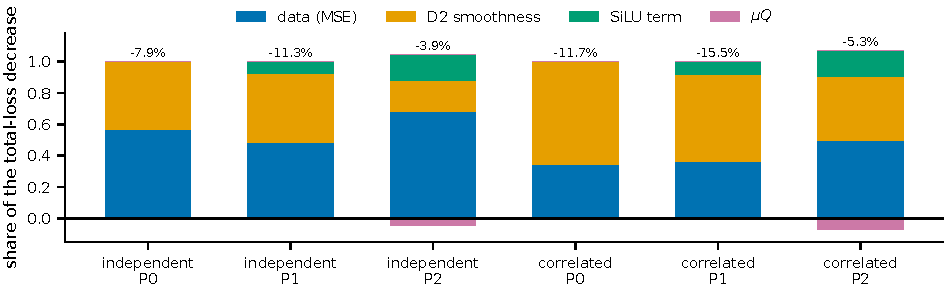
\includegraphics[width=\linewidth]{figS1_lossdecomp.pdf}
  % CAPTION-DRAFT: review (numbers from paper2/figures/figS1_lossdecomp.json)
  \caption{Post hoc loss decomposition (synthetic, early$\to$polished): share of the total-loss decrease from each term, pooled over the 8 seeds of each cell. independent P0: data 0.57, D2 0.43 (median total change -7.9\%); independent P1: data 0.49, D2 0.44 (median total change -11.3\%); independent P2: data 0.68, D2 0.20 (median total change -3.9\%); correlated P0: data 0.35, D2 0.65 (median total change -11.7\%); correlated P1: data 0.37, D2 0.55 (median total change -15.5\%); correlated P2: data 0.50, D2 0.40 (median total change -5.3\%).}
  \label{fig:S1}
\end{figure}


\begin{figure}[h]
  \centering
  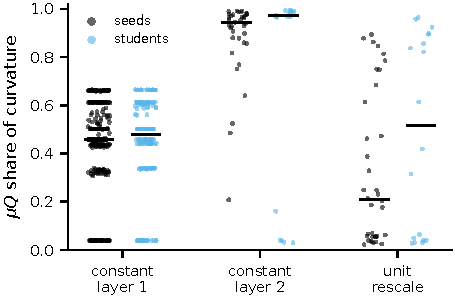
\includegraphics[width=0.5\linewidth]{figS2_gaugecheck.pdf}
  % CAPTION-DRAFT: review (numbers from paper2/figures/figS2_gaugecheck.json)
  \caption{Post hoc gauge check at the $\mu = 10^{-4}$ certified minima: share of the curvature along each least-squares gauge direction contributed by $\mu Q$. Medians: constant shift in layer 1, real-data seeds 0.46 ($n = 288$); constant shift in layer 1, students (trained on a frozen teacher) 0.48 ($n = 144$); constant shift in layer 2, real-data seeds 0.94 ($n = 36$); constant shift in layer 2, students 0.97 ($n = 18$); unit rescaling, real-data seeds 0.21 ($n = 36$); unit rescaling, students 0.52 ($n = 18$).}
  \label{fig:S2}
\end{figure}


\begin{figure}[h]
  \centering
  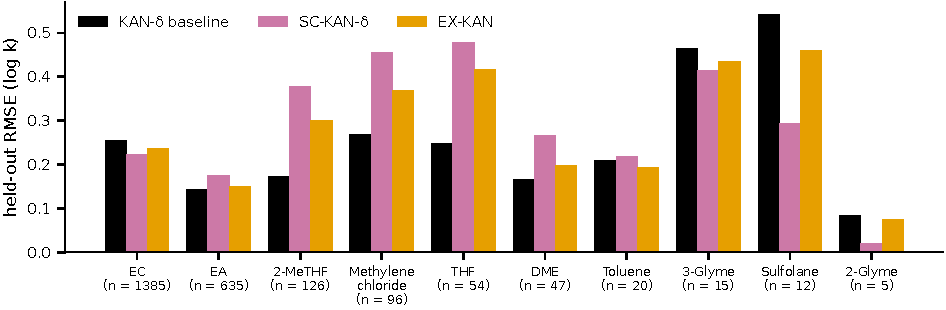
\includegraphics[width=\linewidth]{figS3_loco.pdf}
  % CAPTION-DRAFT: review (numbers from paper2/figures/figS3_loco.json)
  \caption{Leave-one-co-solvent-out RMSE per fold (5-seed ensembles, early state) for the KAN-$\delta$ baseline, SC-KAN-$\delta$ and EX-KAN. Unweighted means: KAN-$\delta$ baseline 0.2554; SC-KAN-$\delta$ 0.2923; EX-KAN 0.2834. The EA fold uses the fold A rows.}
  \label{fig:S3}
\end{figure}

\clearpage  % flush Appendix E's figures before Appendix F
\fi

\end{document}
.
% Generated parts (do not edit by hand; run build_tex.py): title.tex, body.tex, appendixA-E.tex.
\documentclass[10pt]{article}
\ifdefined\PREPRINT
  \usepackage[preprint]{tmlr}
\else
  \usepackage{tmlr}
\fi
\usepackage[utf8]{inputenc}
\usepackage{amsmath,amssymb}
\usepackage{graphicx}
\usepackage{booktabs}
\usepackage{longtable}
\usepackage{array}
\usepackage{url}
\usepackage[hidelinks]{hyperref}
\graphicspath{{../figures/}}
\newcolumntype{R}[1]{>{\raggedright\arraybackslash}p{#1}}

\title{Runaway edges: a smoothness-penalty blind spot makes Kolmogorov--Arnold networks non-identifiable on correlated inputs}


\ifdefined\PREPRINT
  \author{\name Gelavizh Ahmadi \\
          \addr Independent researcher, Berlin, Germany \\
          \addr ORCID: 0000-0000-0000-0000 % ORCID-PLACEHOLDER: replace before posting
          }
  \newcommand{\figname}[1]{(\texttt{#1})}
  \newcommand{\REPOSTATEMENT}{Code, committed results and figure scripts: \url{https://github.com/drgelavizhahmadi-dotcom/battery_hacketon}.}
  \hypersetup{pdftitle={Runaway edges: a smoothness-penalty blind spot makes Kolmogorov-Arnold networks non-identifiable on correlated inputs},
              pdfauthor={Gelavizh Ahmadi}}
\else
  % anonymous build: no author, affiliation, acknowledgments or repository URL anywhere in the source that reaches the PDF
  \author{}
  \newcommand{\figname}[1]{}
  \newcommand{\REPOSTATEMENT}{Code will be released upon publication.}
  \hypersetup{pdftitle={Runaway edges: a smoothness-penalty blind spot makes Kolmogorov-Arnold networks non-identifiable on correlated inputs},
              pdfauthor={}, pdfsubject={}, pdfkeywords={}, pdfcreator={LaTeX}}
\fi

\begin{document}
\maketitle

% GENERATED by build_tex.py from paper2/draft/paper2_draft.md -- do not edit by hand
\begin{abstract}
Kolmogorov--Arnold networks (KANs) are promoted as interpretable because each edge carries a learned univariate function. We show that a widely used family of smoothness penalties leaves a blind spot that undermines this promise: second-difference and curvature penalties do not charge for affine components of an edge, and SiLU base weights are often unpenalised. When the inputs to a layer are correlated, affine components on different edges can cancel inside a unit, so training inflates the parameters along directions that neither the penalty nor the data can see; the loss has no reachable finite minimum and independent runs never agree. In a pre-registered synthetic study with a known teacher, correlated inputs gave 0 of 16 converged models (median squared-norm growth 32--66$\times$), including under a recently proposed curvature penalty that also penalises the SiLU weight, while a small penalty on the affine null space gave 16 of 16 certified minima and exact recovery of the teacher's internals. On real electrolyte-conductivity data the same mechanism explains why no model converged, and polishing beyond early stopping under a weak null-space penalty degraded held-out accuracy (RMSE 0.142 $\to$\allowbreak{} 1.03). Closing the blind spot restores certified minima but leaves several distinct minima, so convergence and identifiability are separate problems. We give practical recommendations for penalised KANs.

\end{abstract}

\section{Introduction}\label{sec:1}

KANs replace a network's fixed activations with learned univariate functions on every edge. Their appeal for science rests on reading those functions: an edge that looks like an exponential decay suggests a physical law. That reading presumes the edges are determined by the data. If different training runs produce different edges with equally good predictions, the edges describe the optimiser, not the system.

This paper identifies a concrete, common mechanism that breaks that presumption. It arises from the interaction of three ingredients that are each standard in practice:

\begin{enumerate}
  \item \textbf{A smoothness penalty with an affine null space.} Second-difference (P-spline) penalties and curvature penalties ignore straight-line components of an edge; SiLU base terms are frequently unpenalised.
  \item \textbf{Correlated inputs to a layer.} Physical descriptors often move together. Hidden units can also become correlated during training, exposing the next layer.
  \item \textbf{Training toward convergence.} Early stopping hides the problem; longer optimisation exposes it.
\end{enumerate}

Together they create directions along which edges grow into large, mutually cancelling affine shapes. The penalty does not see them, and on the training data their contributions cancel. The loss keeps decreasing slightly along these directions, so it has no reachable finite minimum. Seeds wander apart, no model certifies as converged, and on inputs off the training correlation pattern the cancellation fails.

\textbf{Contributions.}

\begin{itemize}
  \item We describe the mechanism and show that it applies to any layer whose inputs are correlated, including the output layer (Section 3).
  \item In a pre-registered synthetic study, we show causally that a recently proposed curvature penalty does not prevent the runaway on correlated inputs, while a small additional penalty on the affine null space prevents it and restores exact recovery of a known solution (Section 4).
  \item On real electrolyte-conductivity data, we trace a complete failure to converge to this mechanism and document its effect on extrapolation (Section 5).
  \item We show that closing the blind spot yields certified, isolated minima but not uniqueness, and that structured alternatives trade accuracy for stability (Section 6).
  \item We give recommendations for penalised KANs (Section 7).
\end{itemize}

All experiments were pre-registered: predictions, thresholds and interpretation rules were committed before the code that tested them. Of 65 predictions in the real-data case study, 11 held, 22 failed and 32 were inconclusive; we report them as recorded.

\section{Background and related work}\label{sec:2}

\textbf{KAN edges.} A KAN layer maps inputs to outputs by summing learned univariate functions, one per edge. In the original formulation \citep{liu2025kan} each edge is a SiLU base term plus a B-spline expansion. FastKAN \citep{li2024fastkan} approximates the B-splines with Gaussian radial basis functions on fixed centres, which is the edge type used in our experiments:

\begin{equation}
  \varphi(x) = \alpha\,\mathrm{SiLU}(x) + \sum_{k=1}^{K} c_k \exp\!\left(-\left(\frac{x-\mu_k}{h}\right)^{2}\right)
\end{equation}

\textbf{Smoothness penalties and their null spaces.} P-spline penalties charge squared second differences of the coefficients \citep{eilers1996psplines}. Constant and linear coefficient patterns cost nothing: the penalty's null space is affine. In generalised additive models this is well understood, and \citet{marra2011double} proposed an additional penalty on the null space (the "double penalty") for variable selection. Our fix is the same construction; what is new is its consequence inside a KAN, where edges are summed within units and passed through further layers.

\textbf{Curvature penalties for KANs.} \citet{bagrow2026curvature} proposed per-edge curvature penalties for compositional smoothness, combining the second-difference penalty with a term $K_{\mathrm{silu}}\,\alpha^{2}$ on the SiLU weight, and noted that the penalty has affine functions as its null space by design. That work evaluated on independent, uniformly sampled inputs. Second-derivative penalties on spline coefficients also appear in other KAN variants, typically on the spline part only, leaving the SiLU base term free (\citealp{cang2024kanwork}; see also the free-knots KAN of \citealp{zheng2025freeknots}). We show that the affine null space becomes a runaway direction when inputs are correlated, and that penalising the SiLU weight alone does not close it.

\textbf{Concurvity.} In additive models, correlated inputs let one input's shape function absorb another's, making shape functions non-identifiable; this is known as concurvity. \citet{siems2023concurvity} proposed a regulariser penalising correlations between transformed features. The cross-edge cancellation we describe is concurvity inside a KAN unit. In an additive model with a penalised null space it shifts shape between functions; combined with an unpenalised affine null space in a KAN, it becomes unbounded growth.

\textbf{Losses without a finite minimum.} When a loss attains its infimum only at infinity, gradient descent drives the parameter norm to diverge, slowly, and optimisation can continue while held-out performance worsens \citep{soudry2018implicit}. Our runaway is an instance of this behaviour created by a penalty's null space.

\textbf{Parameter-space symmetries.} Exact symmetries (unit permutations, sign flips) make parameters non-identifiable in tanh and RBF networks, and completeness results characterise them \citep{sussmann1992uniqueness,kurkova1994uniqueness}. KANs add continuous symmetries such as affine reparametrisations of hidden units. The runaway is not an exact symmetry: it is an approximate one, a nearly flat but tilted direction, which is what prevents convergence.

\section{Mechanism}\label{sec:3}

Consider a unit that sums edges from two inputs, $s = \varphi_1(x_1) + \varphi_2(x_2)$, each edge as in Section 2, trained with a second-difference penalty on its RBF coefficients.

\textbf{Step 1: a direction the penalty cannot see.} Add a linear pattern $t\,\ell$ to the RBF coefficients of edge 1 and subtract it from edge 2, with $\ell_k$ proportional to the centre index. Linear coefficient patterns have zero second difference, so the penalty is unchanged for every t (Figure~\ref{fig:mechanism}b). With Gaussian bumps on a regular grid, the pattern produces a nearly affine function: over the central 80\% of the input range it deviates from a straight line by at most 2\% of its range (Figure~\ref{fig:mechanism}a), and by up to 13\% near the grid edges. Edge 1 thus gains approximately $t\,a\,x_1$ and edge 2 loses $t\,a\,x_2$.

\textbf{Step 2: a direction the data cannot see.} The unit's pre-activation changes by approximately $t\,a\,(x_1 - x_2)$. If $x_{1}$ and $x_{2}$ are strongly correlated, $x_1 - x_2$ is small wherever the data lie, so predictions change little even for large t (Figure~\ref{fig:mechanism}c). The direction is nearly free in both the penalty and the data.


\begin{figure}[t]
  \centering
  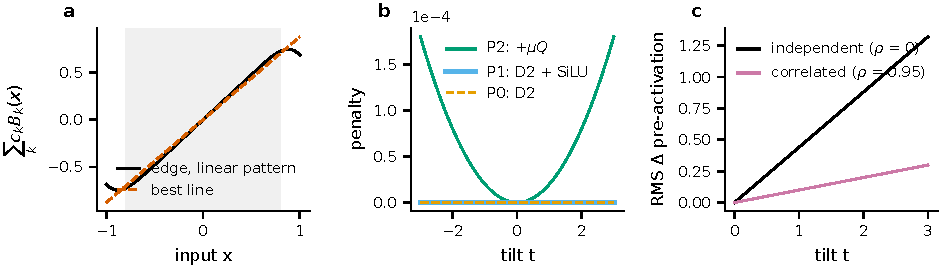
\includegraphics[width=\linewidth]{fig1_mechanism.pdf}
  % CAPTION-DRAFT: review (numbers from paper2/figures/fig1_mechanism.json)
  \caption{Mechanism (computed illustration) for the edge type of Section~\ref{sec:2} (8 Gaussian RBFs on $[-1, 1]$). \textbf{(a)} Edge function produced by a unit linear coefficient pattern and its best straight line; the shaded band is the central 80\% of the range, where the maximum deviation is 2.0\% of the function's range (12.9\% over the full range). \textbf{(b)} Penalty as a function of a tilt $t$ applied as $+t$ to edge 1 and $-t$ to edge 2: the second-difference penalty (P0) and P1 are exactly zero for every $t$; only P2's term $\mu Q$ grows ($\lambda = 0.001$, $\mu = 1e-05$). \textbf{(c)} RMS change in the unit's pre-activation per unit tilt: 0.0996 on correlated inputs ($\rho = 0.95$) against 0.4403 on independent inputs (4.42$\times$).}
  \label{fig:mechanism}
\end{figure}

\textbf{Step 3: no finite minimum.} "Nearly free" is not "free". Moving along it lets the model shed curvature into the free affine and SiLU components, so the loss decreases monotonically along the direction. Both terms contribute (post-hoc decomposition). In the synthetic runaway models the smoothness penalty fell to about a quarter of its early value and supplied a median 61\% of the decrease, while training error fell only 5\%. On real data, from early stopping to the capped state, the penalty fell 8--88$\times$ but supplied 17--36\% of the decrease, the data term the rest. In both, the growth went into whatever the penalty left free: the linear part of the RBF coefficients grew 34--40$\times$ in the synthetic runaway cells, and the SiLU weights 85$\times$ where they were unpenalised. In 12 of 20 synthetic runaway models, training error fell while test error rose. The infimum lies at infinity: gradients stay small but non-zero, the parameter norm grows without bound, and no minimum can be certified. Different seeds drift along different such directions.

\textbf{Step 4: any layer can be affected.} The argument needs only correlated inputs to a layer. Hidden units can become correlated during training, and then the output layer can host the same runaway even when the raw inputs are independent. Correlated hidden units appear necessary for this but not sufficient: they also occur in models that converge once the null space is penalised. Section 4 shows both forms.

\textbf{Consequences.}

\begin{itemize}
  \item \textbf{Non-identifiability:} edges differ across seeds by large affine components that leave predictions almost unchanged.
  \item \textbf{Non-convergence:} second-order optimisers stall; certification criteria fail.
  \item \textbf{Extrapolation risk:} off the training correlation pattern, $x_1 - x_2$ is no longer small, and the inflated components stop cancelling.
\end{itemize}

\textbf{The fix.} Penalise the null space directly. For each edge, let $P_{\mathrm{null}}$ project its RBF coefficients onto constant-plus-linear patterns in the centre index, and add

\begin{equation}
  Q = \sum_{e} \lVert P_{\mathrm{null}}\, c_e \rVert^{2}
\end{equation}

with a small weight $\mu$, in addition to a penalty on the SiLU weight. This makes every affine component cost something, which turns the infinite descent into a finite minimum.

\section{Controlled study}\label{sec:4}

\textbf{Design.} A teacher KAN [4, 3, 1] with smooth, hand-specified edges (fitted by smoothness-penalised least squares) generates targets with Gaussian noise of 5\% of the output spread; n = 2000 training rows. Inputs are $\mathcal{N}(0, 1)/3$, clipped to the grid, either independent or correlated in pairs ($\rho$ = 0.95 for $x_1/x_2$ and $x_3/x_4$). Students share the teacher's architecture and are trained under three penalty levels:

\begin{itemize}
  \item \textbf{P0:} second-difference penalty on RBF coefficients ($\lambda$ = $10^{-3}$).
  \item \textbf{P1:} P0 plus $K_{\mathrm{silu}}\,\alpha^{2}$ on each SiLU weight (Bagrow-style curvature penalty, $K_{\mathrm{silu}}$ = 0.443).
  \item \textbf{P2:} P1 plus $\mu Q$, the affine null-space penalty.
\end{itemize}

Each of the 6 cells has 8 seeds. Each student is trained with AdamW and early stopping, then polished with an exact-Hessian trust-region method and certified by a second-order criterion (gradient, curvature and Newton decrement). $\mu$ was calibrated before the experiment by a pre-registered rule: $10^{-6}$ failed the pilot (5.0$\times$ growth) and $10^{-5}$ passed (1.32$\times$) and was frozen.

\textbf{The teacher itself runs away.} Polished under P0 and P1 on correlated inputs, the teacher's parameters grew 85$\times$ and 1069$\times$ without certifying, while its predictions stayed within half a noise standard deviation of the original. The runaway changes the parameters, not the function.

\begin{table}[t]
  \centering
  % CAPTION-DRAFT: review
  \caption{Synthetic $2\times3$ study, per cell.}
  \label{tab:synthetic}
  \small
  \begin{tabular}{lp{0.2\linewidth}p{0.2\linewidth}p{0.2\linewidth}p{0.2\linewidth}p{0.2\linewidth}p{0.2\linewidth}p{0.2\linewidth}p{0.2\linewidth}p{0.2\linewidth}p{0.2\linewidth}p{0.2\linewidth}p{0.2\linewidth}p{0.2\linewidth}p{0.2\linewidth}p{0.2\linewidth}p{0.2\linewidth}p{0.2\linewidth}p{0.2\linewidth}p{0.2\linewidth}p{0.2\linewidth}p{0.2\linewidth}p{0.2\linewidth}p{0.2\linewidth}p{0.2\linewidth}p{0.2\linewidth}p{0.2\linewidth}p{0.2\linewidth}p{0.2\linewidth}p{0.2\linewidth}p{0.2\linewidth}p{0.2\linewidth}p{0.2\linewidth}p{0.2\linewidth}p{0.2\linewidth}p{0.2\linewidth}p{0.2\linewidth}p{0.2\linewidth}p{0.2\linewidth}p{0.2\linewidth}p{0.2\linewidth}p{0.2\linewidth}p{0.2\linewidth}p{0.2\linewidth}p{0.2\linewidth}p{0.2\linewidth}p{0.2\linewidth}p{0.2\linewidth}p{0.2\linewidth}p{0.2\linewidth}p{0.2\linewidth}p{0.2\linewidth}p{0.2\linewidth}p{0.2\linewidth}p{0.2\linewidth}p{0.2\linewidth}p{0.2\linewidth}p{0.2\linewidth}p{0.2\linewidth}p{0.2\linewidth}}
  \toprule
  Cell & Norm growth & Certified & Unit match to reference \\
  \midrule
  Independent, P0 & 12.5$\times$ & 6/8 & 1.000 \\
  Independent, P1 & 7.9$\times$ & 6/8 & 1.000 \\
  Independent, P2 & 1.09$\times$ & 8/8 & 1.000 \\
  Correlated, P0 & 65.7$\times$ & 0/8 & 0.774 \\
  Correlated, P1 & 32.1$\times$ & 0/8 & 0.883 \\
  Correlated, P2 & 1.00$\times$ & 8/8 & 1.000 \\
  \bottomrule
  \end{tabular}
\end{table}

Medians over 8 seeds; growth is the squared parameter norm, polished over early-stopped.

\textbf{Results.}

\begin{itemize}
  \item \textbf{The published-style penalty does not prevent the runaway.} Penalising the SiLU weight (P1) halved the growth on correlated inputs but left 0 of 8 models certified (Figure~\ref{fig:synthetic}).
  \item \textbf{Closing the null space prevents it everywhere.} P2 gave 16 of 16 certified models with no growth, in both input conditions.
  \item \textbf{Without the runaway, the internals are recoverable.} Every cell without a runaway matched the reference's units and edges exactly (1.000), with seed-to-seed differences around $10^{-4}$.
  \item \textbf{Independent inputs are not fully safe.} Under P0 and P1, most independent seeds grew substantially (8--12$\times$) but settled at certified minima; 4 of 16 (seeds 0 and 4 in each cell) never certified.
\end{itemize}


\begin{figure}[t]
  \centering
  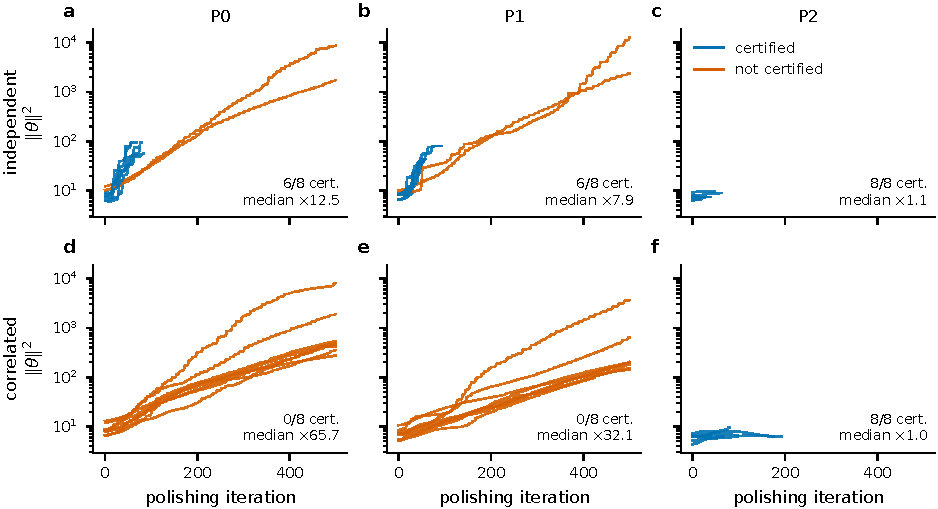
\includegraphics[width=\linewidth]{fig2_synthetic.pdf}
  % CAPTION-DRAFT: review (numbers from paper2/figures/fig2_synthetic.json)
  \caption{Synthetic $2\times3$ study: $\|\theta\|^2$ over trust-exact polishing iterations (log scale), one line per seed, coloured certified (blue) or not certified (vermillion). Rows: independent and correlated inputs; columns: P0, P1, P2. Per panel, certified seeds and median growth (polished over early-stopped): independent P0: 6/8 certified, $\times$12.5; independent P1: 6/8 certified, $\times$7.9; independent P2: 8/8 certified, $\times$1.1; correlated P0: 0/8 certified, $\times$65.7; correlated P1: 0/8 certified, $\times$32.1; correlated P2: 8/8 certified, $\times$1.0.}
  \label{fig:synthetic}
\end{figure}

\textbf{Where the runaway lives.} A post-hoc anatomy of the parameter change shows that in the correlated cells almost all growth sits in the output layer: the layer-1 share of the change was 0.110 (P0) and 0.024 (P1) (Figure~\ref{fig:where}a). It went into the affine part of the output edges' RBF coefficients and, under P0, into their SiLU weights. Cancellation across the edges entering the output rose from about 1.9 to 3.1--3.2, and no hidden unit saturated. The two uncertified independent-P0 seeds put 99.4\% of their change into the output layer. This is Step 4 of Section 3. Among independent-input models, those that ran away were exactly those whose hidden units had become correlated (largest pairwise correlation 0.70, against 0.05 for certified models; Figure~\ref{fig:where}b), while certified P2 models kept correlations up to 0.88 without running away (post-hoc).


\begin{figure}[t]
  \centering
  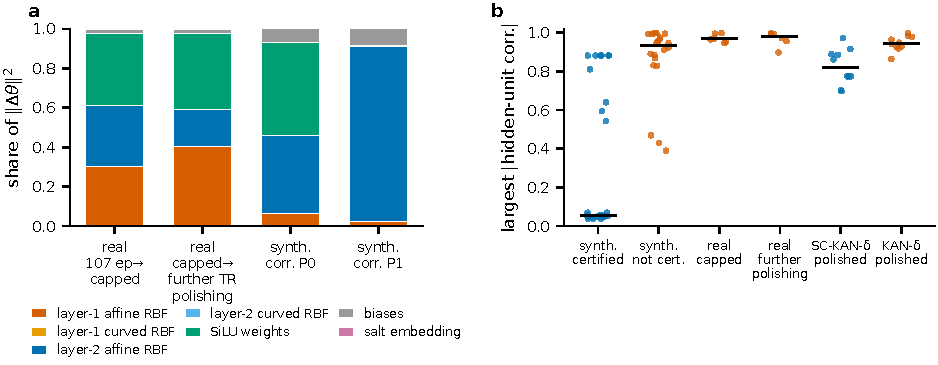
\includegraphics[width=\linewidth]{fig4_where.pdf}
  % CAPTION-DRAFT: review (numbers from paper2/figures/fig4_where.json)
  \caption{Where the runaway lives. \textbf{(a)} Mean share of $\|\Delta\theta\|^2$ by parameter block. Real data, 107 epochs$\to$capped: layer-1 affine RBF 0.30, layer-2 affine RBF 0.31, SiLU weights 0.37; capped$\to$Part~A: 0.40, 0.19, 0.38; synthetic correlated P0: layer-2 affine RBF 0.39, SiLU weights 0.47; correlated P1: layer-2 affine RBF 0.89. The real-data split was evaluated post hoc from archived weights (Appendix~\ref{app:repro}). \textbf{(b)} Largest absolute correlation between hidden-unit activations on the training rows, median: synth. certified 0.054 ($n=28$); synth. not cert. 0.935 ($n=20$); real capped 0.968 ($n=6$); real Part A 0.983 ($n=6$); SC-KAN-$\delta$ polished 0.818 ($n=10$); KAN-$\delta$ polished 0.946 ($n=10$). Blue: certified; vermillion: not certified or runaway.}
  \label{fig:where}
\end{figure}

\textbf{Verdicts.} Of six pre-registered predictions, one held (the certification pattern, X2) and five failed. The failures refine rather than contradict the mechanism. Independent cells exceeded the growth threshold, mostly through finite growth. Cancellation and extrapolation effects were weaker than predicted. Recoverability failed only because the runaway cells were more recoverable than predicted, not less. In this synthetic setting, polishing did not degrade extrapolation: most of the off-pattern error in correlated cells was present at early stopping.

\section{Real-data case study: electrolyte conductivity}\label{sec:5}

\textbf{Task and model.} The CALiSol-23 challenge \citep{deblasio2024calisol} asks for the log conductivity of lithium-ion electrolytes; every test sample contains diethyl carbonate (DEC), which never appears in training. KAN-delta anchors each prediction on the measured conductivity of pure propylene carbonate (PC) and learns only the correction, $\log k = \log k_{\mathrm{PC}} + x_{\mathrm{co}}\, h(z)$, where h is a FastKAN-style network of shape [10, 6, 1]. Its inputs are physical descriptors of the solvents (dielectric constant, log viscosity, molar mass), temperature, molality and a salt embedding. A second-difference penalty acts on the RBF coefficients, and the SiLU weights are unpenalised. Early-stopped after 107 AdamW epochs, it reached RMSE 0.142 on a held-out co-solvent.

\textbf{The inputs are correlated and few-valued.} The three co-solvent descriptors take only 30 distinct combinations in training, and dielectric constant and log viscosity correlate at r = 0.966.

\textbf{Nothing ever converged.}

\begin{itemize}
  \item Of 190 pairs of polished independent seeds, none computed the same function.
  \item After 20,000 float64 L-BFGS iterations, 0 of 26 models converged; exact-Hessian trust-region methods also failed on every seed.
  \item Students trained on a frozen teacher matched its predictions (correlation 0.9988) but not its hidden units (0.66).
\end{itemize}

\textbf{The anatomy matches Section 3.}

\begin{itemize}
  \item From early stopping to the capped state, the squared parameter norm grew 150--1550$\times$ while the smoothness penalty fell 8--88$\times$.
  \item At least 99.9\% of the coefficient change during exact-Newton polishing lay in the penalty's affine null space, in 9 of 9 models.
  \item Cancellation within an edge (SiLU against RBF) stayed small, 1.13--1.33. Cancellation across the edges entering a unit rose from 1.7--2.9 to 4--10, consistent with the correlated descriptors.
  \item The runaway spread across both layers: 30--40\% of the parameter change went into layer-1 affine RBF coefficients, 37--38\% into SiLU weights and 19--31\% into layer-2 affine coefficients (post-hoc), and 12--39\% of hidden units saturated. In the synthetic runaway the output layer dominated.
\end{itemize}

\textbf{Extrapolation suffered.} Polishing beyond early stopping, under a weak null-space penalty, raised the held-out RMSE from 0.142 to 1.03. The cancelling components appear to stop cancelling on the unseen co-solvent, whose descriptors sit off the training correlation pattern. This degradation was much stronger than in the synthetic study, where correlation itself caused most of the off-pattern error; the real model was larger, its norms grew further, and the test solvent lay at the edge of the descriptor range.

\section{Closing the blind spot, and what remains}\label{sec:6}

\textbf{Dose-response on real data.} Adding $\mu Q$ (with the SiLU weights included in Q) and polishing from the early-stopped weights:

\begin{table}[t]
  \centering
  % CAPTION-DRAFT: review
  \caption{Dose-response in $\mu$ on real data (seeds).}
  \label{tab:dose}
  \small
  \begin{tabular}{l l p{0.18\linewidth} l p{0.16\linewidth}}
  \toprule
  $\mu$ & Seeds at a numerical minimum & Negative curvature (seeds) & Norm growth (seeds) & Training fit vs runaway \\
  \midrule
  $10^{-6}$ & 0 of 6 & up to 9 eigenvalues & 21--31$\times$ & about equal \\
  $10^{-5}$ & 4 of 6 & up to 4 eigenvalues & 9--43$\times$ & 12--22\% worse \\
  $10^{-4}$ & 6 of 6 & none & 1.6--16$\times$ & 15--39\% worse \\
  \bottomrule
  \end{tabular}
\end{table}

Under a second-order certificate, all six seeds at $\mu$ = $10^{-4}$ were certified (Figure~\ref{fig:dose}). (The originally pre-registered criterion, which required 10 stationary iterations, proved unreachable because the optimiser stops a few iterations after reaching a minimum; the certificate was defined afterwards and is reported alongside the original verdict.) Saturation fell to at most 0.5\% and cross-edge cancellation to 2.2--2.9.


\begin{figure}[t]
  \centering
  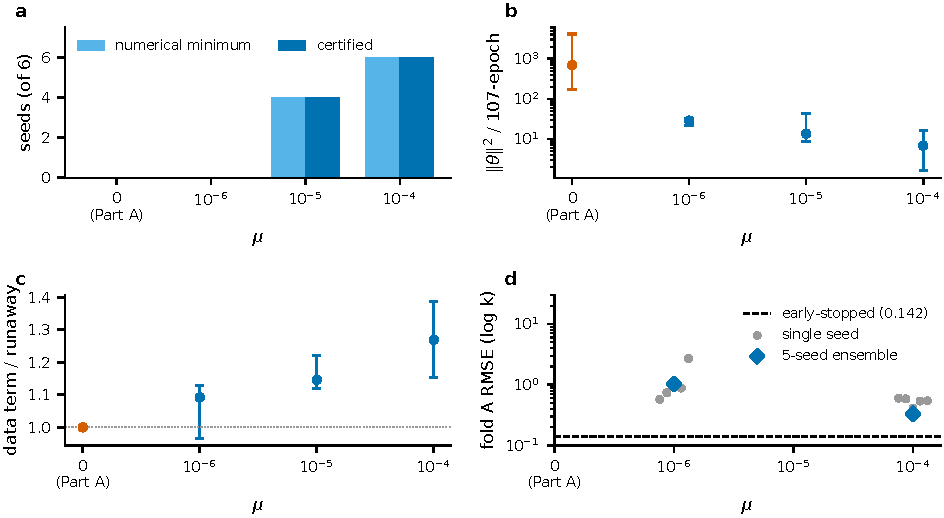
\includegraphics[width=\linewidth]{fig3_dose_response.pdf}
  % CAPTION-DRAFT: review (numbers from paper2/figures/fig3_dose_response.json)
  \caption{Real-data dose-response in the null-space weight $\mu$ (6 KAN-delta seeds; $\mu = 0$ is the runaway reference, stage-2 Part~A). \textbf{(a)} Seeds at a numerical minimum / certified: 0: 0/0; 1e-06: 0/0; 1e-05: 4/4; 0.0001: 6/6. \textbf{(b)} $\|\theta\|^2$ relative to the 107-epoch state, median (range): 0: 690.0 (170.0--4145.5); 1e-06: 28.8 (21.2--31.5); 1e-05: 13.6 (8.6--43.1); 0.0001: 6.8 (1.6--16.0). \textbf{(c)} Training data term relative to the runaway, median: 1e-06: 1.092; 1e-05: 1.146; 0.0001: 1.269. \textbf{(d)} Fold A RMSE: early-stopped 0.142 (dashed line); polished 5-seed ensemble 1.026 at $\mu = 10^{-6}$ and 0.334 at $\mu = 10^{-4}$; grey points are single seeds.}
  \label{fig:dose}
\end{figure}

\textbf{A known solution becomes recoverable.} Under the regularised loss, the original teacher is no longer a minimum. Optimising it under the same loss gives a "regularised teacher" computing nearly the same function (correlation 0.9992). Students match its units at 0.87--0.90 and its edges at 0.97--0.98, against 0.68--0.72 and 0.84--0.91 for the original teacher. This comparison was defined after the results and is exploratory.

\textbf{The penalty acts partly as gauge fixing.} At the certified minima, the layer-2 constant shift, an essentially exact symmetry, owes 96\% of its curvature to $\mu Q$: the regulariser selects one representative. The layer-1 constant shift (46\%) and unit rescaling (24\%) are only approximate symmetries in this architecture, because Gaussian bumps cannot represent constants exactly and tanh breaks rescaling.

\textbf{Convergence is not uniqueness.} Independent seeds at certified minima still disagreed: their median prediction difference fell by only 26\% (Figure~\ref{fig:uniqueness}b). With the runaway removed, the loss has several distinct isolated minima.


\begin{figure}[t]
  \centering
  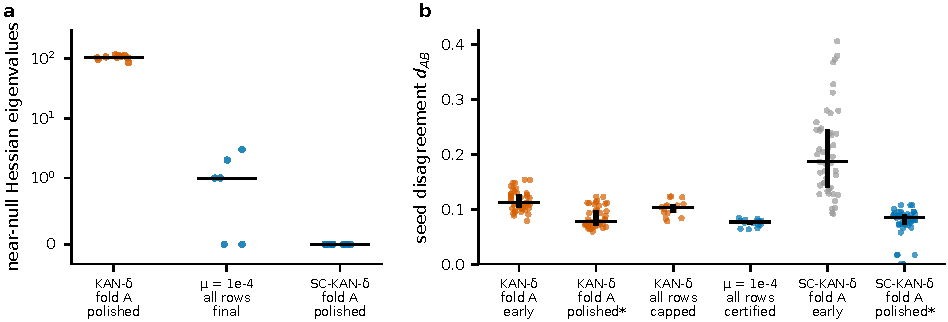
\includegraphics[width=\linewidth]{fig5_uniqueness.pdf}
  % CAPTION-DRAFT: review (numbers from paper2/figures/fig5_uniqueness.json)
  \caption{Convergence is not uniqueness. \textbf{(a)} Near-null Hessian eigenvalues ($|\lambda| < 10^{-8}\lambda_{\max}$) at the end of polishing: KAN-delta baseline on fold A, median 106 (range 86--116); null-space penalty $\mu = 10^{-4}$ on all rows, median 1 (range 0--3); SC-KAN-delta on fold A, 0--0. \textbf{The baseline counts are taken at non-stationary points}: none of the 10 baseline models was certified, and all stopped at the 500-iteration cap. \textbf{(b)} Seed disagreement $d_{AB}$ (median, interquartile range): KAN-$\delta$ fold A early 0.112; KAN-$\delta$ fold A polished$^*$ 0.077; KAN-$\delta$ all rows capped 0.104; $\mu$ = 1e-4 all rows certified 0.077; SC-KAN-$\delta$ fold A early 0.187; SC-KAN-$\delta$ fold A polished$^*$ 0.085. Groups marked $^*$ (polished fold A) are not in any committed result: they were evaluated post hoc from the archived polished weights (SHA-verified; predictions on the 1434 fold A training rows), without any re-optimisation.}
  \label{fig:uniqueness}
\end{figure}

\textbf{Extrapolation.} On the held-out co-solvent, RMSE was 0.142 for the early-stopped model, 1.026 after polishing at $\mu$ = $10^{-6}$ and 0.33 at $\mu$ = $10^{-4}$. Bounding the runaway recovers most of the damage, but early stopping remains the most accurate choice.

\textbf{Structured alternatives.} We tested two architectures designed to remove runaway routes by construction, against the early-stopped baseline, with leave-one-co-solvent-out (LOCO) validation:

\begin{table}[t]
  \centering
  % CAPTION-DRAFT: review
  \caption{Structured alternatives against the early-stopped baseline.}
  \label{tab:alternatives}
  \small
  \begin{tabular}{l p{0.24\linewidth} l l p{0.16\linewidth}}
  \toprule
  Model & Idea & LOCO RMSE & Converged & Seed agreement \\
  \midrule
  Baseline KAN-delta & As above & 0.255 & 0/10 & 0.112 \\
  Shared-curve KAN & One curve per input, mixed by penalised weights & 0.292 & 10/10 & 0.187 early; 0.085 polished \\
  Two-anchor excess model & Pure-solvent offset plus $x(1 - x)$ mixing term & 0.283 & not tested & not tested \\
  \bottomrule
  \end{tabular}
\end{table}

Seed agreement is the median prediction difference between seeds (lower is better). The shared-curve model converged every time, ending with no near-flat directions where the baseline had a median of 106 (range 86--116, at non-stationary points; Figure~\ref{fig:uniqueness}a), and it was less accurate. At the early-stopped state its seeds agreed less than the baseline's (the pre-registered comparison); after polishing to certified minima their median disagreement fell to 0.085, with some seed pairs reaching the same minimum (post-hoc). The excess model's "pure co-solvent offset" tracked viscosity rather than dielectric constant (rank correlation $-$0.85, post hoc), reflecting that no training row contains a pure co-solvent.

\section{Recommendations for practitioners}\label{sec:7}

\begin{enumerate}
  \item \textbf{Penalise the affine null space and the SiLU weights.} If a KAN uses a second-difference or curvature penalty, add a small penalty on the constant-plus-linear component of each edge's coefficients and on each SiLU weight, in every layer. Calibrate its weight so it barely moves a known smooth solution.
  \item \textbf{Check input correlations, including between hidden units.} Strongly correlated or few-valued inputs make the first layer vulnerable; any hidden layer can expose the next one.
  \item \textbf{Monitor parameter norms, not only the loss.} Steady norm growth with a slowly falling loss and stubborn gradients is the signature of the runaway. Certify convergence with a second-order criterion rather than assuming it.
  \item \textbf{Do not read edges from unconverged models.} Compare edges across seeds only after removing exact gauge freedoms, and only for models that reached certified minima.
  \item \textbf{Treat seed disagreement as information.} Even at certified minima, distinct solutions can remain. Disagreement then signals that the data do not determine the function, not merely that training was unfinished.
  \item \textbf{Validate on genuinely new conditions.} A held-out fold from the training distribution can understate extrapolation error severalfold; leave-one-group-out validation is closer to the use case.
  \item \textbf{Keep early stopping as a baseline.} In our real-data case it gave the best held-out accuracy of every variant tested.
\end{enumerate}

\section{Limitations and research process}\label{sec:8}

\textbf{Scope.}

\begin{itemize}
  \item One real dataset and one synthetic teacher; small networks ([4, 3, 1] and [10, 6, 1]).
  \item One edge type: Gaussian RBFs on fixed centres with a SiLU base. The argument applies to B-spline KANs with second-difference or curvature penalties, but we did not test them directly.
  \item Our P1 keeps the second-difference penalty on RBF coefficients and adds Bagrow's SiLU term; it is Bagrow-style, not a replication of his RBF curvature form.
  \item The null-space weight used in the shared-curve model was carried over from the synthetic calibration, not re-calibrated.
\end{itemize}

\textbf{Post-hoc elements.} The second-order certificate, the regularised-teacher comparison, the gauge-curvature analysis and both anatomy studies were defined after seeing results. We report them as exploratory and never in place of pre-registered verdicts.

\textbf{Extrapolation.} The strong degradation from polishing appeared on real data but not in the synthetic study, so we do not claim it as a general law.

\textbf{Process.} Each study committed its predictions, thresholds and interpretation rules before its code existed; any later change was dated and recorded as an amendment, and every verdict is linked to the commit that produced it. Several predictions failed or proved untestable as specified; following them up, rather than reinterpreting them, is what led to the mechanism reported here. Experiments were run with an AI coding agent working under this protocol, with a rule that committed files take precedence over any number stated in a prompt.


\bibliography{references}
\bibliographystyle{tmlr}

\appendix
\ifdefined\PREPRINT
  % GENERATED by build_tex.py (preprint: real commit hashes)
\section{All pre-registered predictions}\label{app:prereg}

Generated by \texttt{paper2/tex/build\_tex.py} from the committed verdict sections; the cell text is the committed wording. Each study opens with its pre-registration's title and its committed question (or theory). Commits are given as pre-registration $\to$ results (in the anonymous version, as neutral labels S-NN). Thresholds are part of each prediction's wording.

\subsection{Synthetic controlled study}
\noindent\textit{Pre-registration:} ``Pre-registration: synthetic teacher-student test of the runaway mechanism (paper2/synth)''. \textbf{Teacher and students: KAN [4, 3, 1].} Two stacked \texttt{kan.KANLayer}s with tanh between them, as in \texttt{kan.KAN}, but \textbf{without} the salt embedding that \texttt{kan.KAN} always adds. Same edge type: SiLU base plus 8 Gaussian RBFs on fixed centres linspace($-$1, 1, 8), width 2/7.

{\footnotesize\setlength{\tabcolsep}{3pt}
\begin{longtable}{R{0.07\linewidth} R{0.28\linewidth} R{0.35\linewidth} R{0.09\linewidth} R{0.11\linewidth}}
\toprule
ID & Prediction (threshold) & Result & Verdict & Commits \\
\midrule
\endhead
X1 & runaway ($\geq$ 10) in correlated P0 and P1; $\leq$ 3 in the three independent cells and correlated P2 & Correlated P0 $\times$65.7 and P1 $\times$32.1, and P2 $\times$1.00, as predicted. \textbf{But independent P0 $\times$12.5 and P1 $\times$7.9 exceed 3} (independent P2 $\times$1.09) & \textbf{failed} & dfd281d$\to$\allowbreak 34cc321 \\
X2 & certified $\leq$ 2/8 in correlated P0 and P1; $\geq$ 6/8 elsewhere & correlated P0 0/8, P1 0/8; independent 6/8, 6/8, 8/8; correlated P2 8/8 & \textbf{held} & dfd281d$\to$\allowbreak 34cc321 \\
X3 & cancellation in correlated P0 and P1 each $\geq$ 2 $\times$ correlated P2 & P0 3.29 and P1 2.32, against 2 $\times$ 1.99 = 3.98 & \textbf{failed} & dfd281d$\to$\allowbreak 34cc321 \\
X4 & off-manifold ratio $\geq$ 3 in correlated P0 and P1, $\leq$ 1.5 in P2 & P0 1.22, P1 \textbf{0.77}; P2 0.78 (the P2 part held) & \textbf{failed} & dfd281d$\to$\allowbreak 34cc321 \\
X5 & Spearman(cancellation, off-manifold RMSE) $\geq$ 0.6 over the 24 correlated models & $\rho$ = +0.177, p = 0.407 & \textbf{failed} & dfd281d$\to$\allowbreak 34cc321 \\
X6 & unit match $\geq$ 0.85 in the independent cells and correlated P2; < 0.7 in correlated P0 and P1 & The first part held: 1.000 in all four no-runaway-predicted cells. \textbf{The second part failed: correlated P0 0.774 and P1 0.883 are not < 0.7} & \textbf{failed} & dfd281d$\to$\allowbreak 34cc321 \\
\bottomrule
\end{longtable}}
\subsection{Real-data case study}
\noindent\textit{From the case-study close-out:} KAN-$\delta$ predicts Li-electrolyte conductivity for the CALiSol-23 DEC holdout. Its
prediction is log k = a measured pure-PC anchor + x\_co $\cdot$ h(solvent descriptors, 1/T, molality, salt).
Its first layer is a [8 continuous inputs + 2 salt-embedding, 6, 1] FastKAN, with SiLU + 8 Gaussian
RBFs per edge and a smoothness penalty (\texttt{kan.py}, \texttt{final.py}).

Rows are as committed in the case-study summary (one row may cover several predictions, e.g.\ F2--F5). The rank intervention's verdicts are given per arm in the result column.

{\footnotesize\setlength{\tabcolsep}{3pt}
\begin{longtable}{R{0.14\linewidth} R{0.26\linewidth} R{0.29\linewidth} R{0.10\linewidth} R{0.11\linewidth}}
\toprule
Study & Prediction (threshold) & Result & Verdict & Commits \\
\midrule
\endhead
Gauge study & \textbf{Control 1}: teacher edges recovered, median dense corr $\geq$ 0.8 & 0.301 (sanity: h corr 0.913 < 0.95) & \textbf{failed} & c11dd92$\to$\allowbreak{}e68e2eb \\
Gauge study & P1: gauge fixing removes $\geq$ 50\% of edge variance & not run & inconclusive (gated by Control 1) & c11dd92$\to$\allowbreak{}e68e2eb \\
Gauge study & P2: sparse $\geq$ 2$\times$ dense, DEC region highest & not run & inconclusive (gated) & c11dd92$\to$\allowbreak{}e68e2eb \\
Gauge study & P3: (e) < (d) < (c) < (a) & not run & inconclusive (gated) & c11dd92$\to$\allowbreak{}e68e2eb \\
Gauge study & P4: every seed has a unit with |corr| < 0.8 & not run & inconclusive (gated) & c11dd92$\to$\allowbreak{}e68e2eb \\
Gauge study & P5: KAN-full edge variance > KAN-$\delta$ & not run & inconclusive (gated) & c11dd92$\to$\allowbreak{}e68e2eb \\
Gauge study & P6: seed spread flags errors & Spearman +0.169 (A) / +0.213 (B); fold B RMSE at 80\% coverage 0.153 vs random 0.137 & \textbf{failed} & c11dd92$\to$\allowbreak{}67fe9f2 \\
Control 2 & C1: (I,C) edges $\geq$ 0.9 and units $\geq$ 0.9 & prediction corr 0.947 < 0.99 & inconclusive (gate failed) & 45b336f$\to$\allowbreak{}a260aef \\
Control 2 & C2: (R,C) invT, molal $\geq$ 0.9; co-solvent < 0.7 & prediction corr 0.969 < 0.99 & inconclusive (gate failed) & 45b336f$\to$\allowbreak{}a260aef \\
Control 2 & C3: 107 epochs gives prediction corr < 0.95 & 0.858 (I,S), 0.919 (R,S) & \textbf{held} & 45b336f$\to$\allowbreak{}a260aef \\
Control 3 & C1': (I) passes the gate, edges $\geq$ 0.9, units $\geq$ 0.9 & (I) RMSE/std 0.128 > 0.05; unit match 0.648 & \textbf{failed} & 812a0fa$\to$\allowbreak{}9f59d39 \\
Control 3 & C2': (R) edges $\leq$ (I) edges $-$ 0.10 & (R) edges 0.852, units 0.659 & inconclusive ((I) failed the gate) & 812a0fa$\to$\allowbreak{}9f59d39 \\
Control 3 & C4: every continuous input $\geq$ 0.9 in (I) & -- & inconclusive ((I) failed the gate) & 812a0fa$\to$\allowbreak{}9f59d39 \\
Fiber & F1: $\geq$ 50\% of seed pairs on-fiber & 0/190 (closest d = 0.146) & \textbf{failed} & e83df2e$\to$\allowbreak{}f220a2f \\
Fiber & F2--F5 & not run & inconclusive (no on-fiber pairs) & e83df2e$\to$\allowbreak{}f220a2f \\
Fiber 2 & G1: $\geq$ 4/6 seeds and $\geq$ 10/20 students certify convergence & 0/6, 0/20 (all at the 20,000-iteration cap) & \textbf{failed} & 4af5250$\to$\allowbreak{}98eca9d \\
Fiber 2 & G2--G5 & not run & inconclusive (no converged model) & 4af5250$\to$\allowbreak{}98eca9d \\
Support & H1: dim(N) $\geq$ 5 & dim(N) = 36 of 72 & \textbf{held} & b473232$\to$\allowbreak{}c5505e5 \\
Support & H2: $\geq$ 50\% of N is REDISTRIBUTION within the correlated group & 18/36 & \textbf{held, exactly at threshold} & b473232$\to$\allowbreak{}c5505e5 \\
Support & H3: set A fraction in N $\geq$ 0.5 and $\geq$ 3$\times$ random & median 0.942 (random 0.5) & inconclusive (untestable: 3 $\times$ 0.5 > 1) & b473232$\to$\allowbreak{}c5505e5 \\
Support & H4: set B (capped), same criterion & median 0.949 & inconclusive (untestable) & b473232$\to$\allowbreak{}c5505e5 \\
Support & H5: flattest Hessian directions overlap N $\geq$ 0.5 & median 0.885; median layer-1 block share only 0.08 & \textbf{held}, with caveat (see \texttt{support\_\allowbreak{}prereg.md}) & b473232$\to$\allowbreak{}c5505e5 \\
Support & H6: fraction in N rises from control-3 to capped state, $\geq$ 15/20 & 20/20 (0.713 $\to$\allowbreak{} 0.949) & \textbf{held} & b473232$\to$\allowbreak{}c5505e5 \\
Rule & I1--I5 (gate) & 0 columns removed; gate stopped & inconclusive & 6c93bf4$\to$\allowbreak a53cc2a \\
Rank & I1: median max|grad| $\leq$ 0.1 $\times$ baseline & arm G: \textbf{failed} (4.00$\times$); arm F: \textbf{failed} (29.1$\times$) & see result & df44ead$\to$\allowbreak aeb6f87 \\
Rank & I2: median d\_AB $\leq$ 0.5 $\times$ baseline & arm G: \textbf{failed} (0.945$\times$); arm F: \textbf{failed} (0.808$\times$) & see result & df44ead$\to$\allowbreak aeb6f87 \\
Rank & I3 (sanity): median loss $\leq$ 1.10 $\times$ baseline & arm G: passed (1.004$\times$); arm F: passed, narrowly (1.099$\times$) & see result & df44ead$\to$\allowbreak aeb6f87 \\
Rank & I4: fold A RMSE $\leq$ 0.150 (KAN-$\delta$ 0.1420) & arm G: \textbf{held}, narrowly (0.1499); arm F: \textbf{failed} (0.1587) & see result & df44ead$\to$\allowbreak aeb6f87 \\
Rank & I5: edge corr on 1000/T and molality $\geq$ baseline + 0.1 (baseline 0.102) & arm G: \textbf{held} (0.927); arm F: \textbf{held} (0.338) & see result & df44ead$\to$\allowbreak aeb6f87 \\
Rank & I6: arm F's improvement $\geq$ arm G's in both I1 and I2 & arm G: \textbf{failed} (max|grad| 29.1$\times$ vs 4.00$\times$; d\_AB does favour F, 0.808 vs 0.945) & see result & df44ead$\to$\allowbreak aeb6f87 \\
Trust & T1 / T2: trust-krylov certifies $\geq$ 4/6 seeds / $\geq$ 2/3 students & 0/6, 0/3. All 9 stopped on scipy's "bad approximation" after 1--62 iterations; the Hessian was accurate to $\leq$ $2\times10^{-7}$ & \textbf{failed} & a77e8b4$\to$\allowbreak 67586d6 \\
Trust & T3--T5 & nothing converged & inconclusive & a77e8b4$\to$\allowbreak 67586d6 \\
Stage 2 & U1: trust-exact (exact Hessian, 500 iterations) certifies $\geq$ 4/6 seeds & 0/6. All 9 hit the iteration cap & \textbf{failed} & c6a9e83$\to$\allowbreak b8d6488 \\
Stage 2 & U2: with L2 $\lambda$ = $10^{-5}$, $\geq$ 4/6 seeds and $\geq$ 2/3 students & 1/6 seeds, 0/3 students & \textbf{failed} & c6a9e83$\to$\allowbreak b8d6488 \\
Stage 2 & U3: more converge at $10^{-5}$ than at $10^{-6}$ & 1 vs 0 & \textbf{held} & c6a9e83$\to$\allowbreak b8d6488 \\
Stage 2 & U4: converged L2 models' loss without L2 $\leq$ 1.05 $\times$ capped & 1.2545 & \textbf{failed} & c6a9e83$\to$\allowbreak b8d6488 \\
Stage 2 & U5: converged seeds' disagreement $\leq$ 0.5 $\times$ capped & only 1 converged & inconclusive & c6a9e83$\to$\allowbreak b8d6488 \\
Close & V1: at some $\mu$, $\geq$ 4/6 seeds and $\geq$ 2/3 students converge (stage2 criterion) & 0 certified at every $\mu$ & \textbf{failed} & e5105d7$\to$\allowbreak{}65ed55f \\
Close & V2: converged seeds' data term $\leq$ 1.05 $\times$ stage2 A & nothing certified at the selected $\mu$ = $10^{-6}$ & inconclusive & e5105d7$\to$\allowbreak{}65ed55f \\
Close & V3: $\|\theta\|^{2}$ $\leq$ 10 $\times$ start & same & inconclusive & e5105d7$\to$\allowbreak{}65ed55f \\
Close & V4: seed disagreement halved & same & inconclusive & e5105d7$\to$\allowbreak{}65ed55f \\
Close & V5: students' unit match $\geq$ 0.8 & same & inconclusive & e5105d7$\to$\allowbreak{}65ed55f \\
Close & V6: fold A RMSE $\leq$ 0.150 & 1.0262, bias +0.9028 & \textbf{failed} & e5105d7$\to$\allowbreak{}65ed55f \\
Certify & W1: at $\mu$ = $10^{-4}$, $\geq$ 5/6 seeds certified (second-order criterion, F-a) & 6/6; all 17 candidates certified & \textbf{held} & 5f4520a$\to$\allowbreak{}36f295b \\
Certify & W2: certified seeds' median d\_AB $\leq$ 0.5 $\times$ capped & 0.0771 vs capped 0.1041 ($-$26\%) & \textbf{failed} & 5f4520a$\to$\allowbreak{}36f295b \\
Certify & W3: certified students' unit match $\geq$ 0.8 (vs the original teacher) & 0.624 & \textbf{failed} & 5f4520a$\to$\allowbreak{}36f295b \\
Certify & W4: $\mu$ = $10^{-4}$ fold A RMSE $\leq$ 0.150 & 0.3345 & \textbf{failed} & 5f4520a$\to$\allowbreak{}36f295b \\
Certify & W5: $\mu$ = $10^{-4}$ fold A RMSE $\leq$ 0.5131 & 0.3345 & \textbf{held} & 5f4520a$\to$\allowbreak{}36f295b \\
Certify & W6: Spearman(cross-edge ratio, held-out RMSE) $\geq$ 0.6 & $\rho$ = +0.345, p = 0.328 (weak test) & \textbf{failed} & 5f4520a$\to$\allowbreak{}36f295b \\
\bottomrule
\end{longtable}}
\noindent Committed tally of the case study:

{\footnotesize\setlength{\tabcolsep}{3pt}
\begin{longtable}{R{0.55\linewidth} r r r}
\toprule
Study & Held & Failed & Inconclusive \\
\midrule
\endhead
First table (Control 1, P1--P6, C1--C3, C1'/C2'/C4, F1--F5, G1--G5, H1--H6) & 5 & 5 & 19 \\
Rule (I1--I5) & 0 & 0 & 5 \\
Rank (I1, I2, I4, I5 per arm, I6) & 3 & 6 & 0 \\
Trust (T1--T5) & 0 & 2 & 3 \\
Stage 2 (U1--U5) & 1 & 3 & 1 \\
Close (V1--V6) & 0 & 2 & 4 \\
Certify (W1--W6) & 2 & 4 & 0 \\
\textbf{Total} & \textbf{11} & \textbf{22} & \textbf{32} \\
\bottomrule
\end{longtable}}
\subsection{Shared-curve KAN}
\noindent\textit{Pre-registration:} ``SC-KAN-$\delta$ (shared-curve KAN-$\delta$): pre-registration''. \textbf{Inputs:} the 8 continuous final.py features (flag 11), scaled exactly as in final.py. Salt enters through a learned 2-number embedding e(salt), passed through tanh.

Run after the case-study close-out; not part of the 65 predictions above.

{\footnotesize\setlength{\tabcolsep}{3pt}
\begin{longtable}{R{0.07\linewidth} R{0.28\linewidth} R{0.35\linewidth} R{0.09\linewidth} R{0.11\linewidth}}
\toprule
ID & Prediction (threshold) & Result & Verdict & Commits \\
\midrule
\endhead
S1 & SC LOCO RMSE $\leq$ 1.05 $\times$ baseline & unweighted mean SC 0.2923 vs base 0.2554 (ratio 1.145; threshold 0.2681). Also reported: row-weighted 0.2478 / 0.2297 (1.079); folds $\geq$ 20 rows 0.3138 / 0.2093 (1.499) & failed & 0053d01$\to$\allowbreak e00e37f \\
S2 & SC fold A RMSE $\leq$ 0.160 & SC 0.1757 (base 0.1420) & failed & 0053d01$\to$\allowbreak e00e37f \\
S3 & SC median d\_AB $\leq$ 0.5 $\times$ baseline & SC 0.1865 vs base 0.1120 (threshold 0.0560): SC seeds agree \emph{less} than baseline seeds & failed & 0053d01$\to$\allowbreak e00e37f \\
S4 & curve corr $\geq$ 0.90 for $\geq$ 6 of 8 inputs & 3 of 8 (M\_co 0.959, mix\_lneta 0.970, invT 0.986); lowest x\_co 0.596; others 0.871--0.891 & failed & 0053d01$\to$\allowbreak e00e37f \\
S5 & $\geq$ 8/10 SC fold A models certified & SC 10/10 (max|grad| $\leq$ $7\times10^{-10}$, 0 near-null eigenvalues); baseline 0/10 (all hit the 500-iteration cap) & held & 0053d01$\to$\allowbreak e00e37f \\
S6 & median $\beta$-norm polished/early $\leq$ 3 (calibrated) & median 1.337 (range 0.652--2.356); $\|\theta\|^{2}$ $\times$4.59 (base $\times$67.9, range 30.6--281) & held & 0053d01$\to$\allowbreak e00e37f \\
S7 & SC polished/early fold A RMSE $\leq$ 1.5 & SC 1.920 (0.1757 $\to$\allowbreak{} 0.3373); baseline 5.736 (0.1420 $\to$\allowbreak{} 0.8147) & failed & 0053d01$\to$\allowbreak e00e37f \\
S8 & d log k/d(1000/T) < 0 on $\geq$ 95\% rows in $\geq$ 8/10 seeds & 10/10 (median share 1.000; 1424 rows, 10 excluded per D4) & held & 0053d01$\to$\allowbreak e00e37f \\
S9 & Spearman(1000/T, |slope|) > 0 in $\geq$ 8/10 seeds & 10/10 (median +0.661, range +0.406 to +0.885) & held & 0053d01$\to$\allowbreak e00e37f \\
S10 & d log k/d(ln $\eta$\_mix) < 0 on $\geq$ 90\% rows in $\geq$ 8/10 seeds & 7/10 (median share 0.967; s0 0.892, s2 0.892, s8 0.826) & failed & 0053d01$\to$\allowbreak e00e37f \\
\bottomrule
\end{longtable}}
\subsection{Two-anchor excess model}
\noindent\textit{Pre-registration:} ``EX-KAN (two-anchor excess model): pre-registration''. log k = anchor\_PC + x\_co $\cdot$ s(eps\_co, ln\_eta\_co, M\_co, 1000/T) + x\_co $\cdot$ (1 $-$ x\_co) $\cdot$ g(eps\_co, ln\_eta\_co, M\_co, 1000/T, molality, salt) So $\delta$ = log k $-$ anchor\_PC = x\_co $\cdot$ [s + (1 $-$ x\_co) $\cdot$ g].

Run after the case-study close-out; not part of the 65 predictions above.

{\footnotesize\setlength{\tabcolsep}{3pt}
\begin{longtable}{R{0.07\linewidth} R{0.28\linewidth} R{0.35\linewidth} R{0.09\linewidth} R{0.11\linewidth}}
\toprule
ID & Prediction (threshold) & Result & Verdict & Commits \\
\midrule
\endhead
E1 & EX LOCO $\leq$ 0.95 $\times$ KAN-$\delta$ & unweighted mean EX 0.2834 vs threshold 0.2426 (base 0.2554; ratio 1.110). Row-weighted 0.2363 / 0.2297 (1.029); folds $\geq$ 20 rows 0.2662 / 0.2093 (1.272). EX is better on EC (0.237 vs 0.256), Sulfolane, 3-Glyme, 2-Glyme and Toluene, and worse on 2-MeTHF, THF, Methylene chloride, DME and EA & failed & 3938f8f$\to$\allowbreak 579b58f \\
E2 & EX fold A $\leq$ 0.142 & EX 0.1502 (base this run 0.1420) & failed & 3938f8f$\to$\allowbreak 579b58f \\
E3 & s agrees across seeds (separable co-solvents, Amendment 1) & median pairwise corr +0.987 over EA, EC, Methylene chloride: a weak test with 3 values per seed, and Methylene chloride is marginal. Seed SD of s: EA 0.063 (0.39 $\times$ the spread across co-solvents, 0.159), EC 0.091 (0.57 $\times$), Methylene chloride 0.067 (0.42 $\times$). Secondary ($\leq$ 2 rule, 7 co-solvents): +0.869 & held & 3938f8f$\to$\allowbreak 579b58f \\
E4 & mean s(low $\varepsilon$) < mean s(EC, Sulfolane) in $\geq$ 8/10 seeds & 0/10: the ordering is reversed in every seed. Per high-$\varepsilon$ co-solvent: vs EC alone 0/10 (EC median s +0.104), vs Sulfolane alone 0/10 (median $-$0.124). The low-$\varepsilon$ mean is +0.19 to +0.49 per seed. Sulfolane does not drive the failure on its own: EC alone fails in every seed too & failed & 3938f8f$\to$\allowbreak 579b58f \\
E5 & median seed-SD flagged $\geq$ 2 $\times$ separable (Amendment 1) & 0.091 vs 0.067, ratio 1.37. Secondary ($\leq$ 2 rule): 0.222 vs 0.069, ratio 3.22, no verdict; the secondary is driven by 3-Glyme (SD 0.478, M\_co extrapolated) and 2-Glyme (0.222) & failed & 3938f8f$\to$\allowbreak 579b58f \\
\bottomrule
\end{longtable}}
\paragraph{Revision studies.} The studies below were run for the revision, each with its own pre-registration.

\subsection{Freeze test: is composition necessary? (and weight decay)}
\noindent\textit{Pre-registration:} ``Revision step 2: is composition necessary? (plus weight decay)''. With layer 1 fixed, the output is linear in the layer-2 parameters: a fixed basis times coefficients. The data term plus a quadratic penalty is then a convex quadratic. It can have flat directions but no tilted ones, so it cannot run away. If the runaway needs composition, freezing layer 1 should remove it.

{\footnotesize\setlength{\tabcolsep}{3pt}
\begin{longtable}{R{0.07\linewidth} R{0.28\linewidth} R{0.35\linewidth} R{0.09\linewidth} R{0.11\linewidth}}
\toprule
ID & Prediction (threshold) & Result & Verdict & Commits \\
\midrule
\endhead
Z1 & Arm A certified: $\geq$ 5/6 real; $\geq$ 7/8 in each synthetic cell & A-R 6/6; A-S correlated P0 8/8; A-S correlated P1 8/8 & HELD & a6d752b$\to$\allowbreak 9228f70 \\
Z2 & Arm A median layer-2 growth $\leq$ 3 in R and in each synthetic cell & A-R $\times$582.8 ($\times$206--$\times$11,689); P0 $\times$4.07 ($\times$1.36--$\times$245); P1 $\times$22.9 ($\times$1.51--$\times$801) & FAILED & a6d752b$\to$\allowbreak 9228f70 \\
Z3 & Arm A smallest Hessian eigenvalue $\geq$ $-10^{-8}$ $\times$ largest at every logged iterate & worst ratio +$1.99\times10^{-10}$ (all values positive) & HELD & a6d752b$\to$\allowbreak 9228f70 \\
Z4 & Arm C: 8/8 certified, median growth $\leq$ 3 & 8/8; $\times$2.52 ($\times$1.68--$\times$2.85) & HELD (computed before the stop) & a6d752b$\to$\allowbreak 9228f70 \\
Z5 & Arm D branch & 8/8 certified; median growth $\times$0.415 ($\times$0.263--$\times$0.540). Note: this rule uses the same $\leq$ 3 growth threshold as Z2 and shares its weakness (see the interpretation note); here the norm shrinks, so the threshold is not binding. & "an L2 term of this size at polish time bounds the runaway" & a6d752b$\to$\allowbreak 190544d \\
Z6 E(i) & Arm E, synthetic correlated P0 & median $\|\theta\|^{2}$ ratio wd 0 / wd $10^{-4}$ $\times$1.0011 ($\times$0.987--$\times$1.007); in-distribution RMSE 0.0091 vs 0.0091; off-manifold 0.0667 vs 0.0665; determinism check max |diff| 0 & "early stopping alone kept them bounded; weight decay was incidental" & a6d752b$\to$\allowbreak 190544d \\
Z6 E(ii) & Arm E, real fold A & median ratio $\times$1.0001 ($\times$1.0001--$\times$1.0001); fold A ensemble RMSE 0.1420 vs 0.1420; determinism check max |diff| 0 & "early stopping alone kept them bounded; weight decay was incidental" & a6d752b$\to$\allowbreak 190544d \\
\bottomrule
\end{longtable}}
\subsection{Infimum test: a certified regularisation path}
\noindent\textit{Pre-registration:} ``Revision step 3: infimum test (a certified L2 regularisation path)''. Does the unregularised loss of the full model have a finite minimum that is merely distant? Or does its infimum lie at infinity (a receding minimum)?

Predictions I1--I4 apply per phase (Phase 1 synthetic, Phase 2 real data); the real-data control arm was added after Phase 2 with its outcomes fixed before it ran.

{\footnotesize\setlength{\tabcolsep}{3pt}
\begin{longtable}{R{0.07\linewidth} R{0.28\linewidth} R{0.35\linewidth} R{0.09\linewidth} R{0.11\linewidth}}
\toprule
ID & Prediction (threshold) & Result & Verdict & Commits \\
\midrule
\endhead
I1 & Phase 1: runaway: $\|\theta^{*}\|^{2}$ increases as $\gamma$ decreases & 16/16 & HELD & 179814f$\to$\allowbreak ef3b3c2 \\
I2 & Phase 1: runaway: $\alpha$ > 0.2, bootstrap 95\% interval excluding 0 & 16/16 & HELD & 179814f$\to$\allowbreak ef3b3c2 \\
I3 & Phase 1: control: ratio between the two smallest certified $\gamma$ $\leq$ 1.5 & 8/8 & HELD & 179814f$\to$\allowbreak ef3b3c2 \\
I4 & Phase 1: runaway: $L^{*}$ decreases as $\gamma$ decreases & 16/16 & HELD & 179814f$\to$\allowbreak ef3b3c2 \\
I1 & Phase 2: runaway: $\|\theta^{*}\|^{2}$ increases as $\gamma$ decreases & 6/6 & HELD & 179814f$\to$\allowbreak 349022b \\
I2 & Phase 2: runaway: $\alpha$ > 0.2, bootstrap 95\% interval excluding 0 & 6/6 & HELD & 179814f$\to$\allowbreak 349022b \\
I3 & Phase 2: discrimination check & --- & Phase 1's I3 (HELD, 8/8), as pre-registered; Phase 2 has no control models & 179814f$\to$\allowbreak 349022b \\
I4 & Phase 2: runaway: $L^{*}$ decreases as $\gamma$ decreases & 6/6 & HELD & 179814f$\to$\allowbreak 349022b \\
Control & Post hoc, outcomes fixed before running. Plateau: the $\|\theta^{*}\|^{2}$ ratio between the two smallest certified (incl. certified-degenerate) $\gamma$ values is $\leq$ 1.5 for both seeds. The real-data contrast is then complete. & The $\|\theta^{*}\|^{2}$ ratio between the two smallest certified $\gamma$ is 1.092 (ind0) and 1.101 (ind1), both $\leq$ 1.5, so the real-data contrast is complete. The divergence condition is not met: $\alpha$ is +0.105 [+0.093, +0.118] and +0.124 [+0.109, +0.139], both below 0.2. & plateau & 349022b$\to$\allowbreak 4003b21 \\
\bottomrule
\end{longtable}}
\subsection{Correlation dose-response}
\noindent\textit{Pre-registration:} ``Revision step 4: dose-response --- how much correlation does the blind spot need?''. At what input correlation does the runaway turn on, and does the null-space penalty still close it at the strongest dose?

Verdict column: P0 / P1. The thresholds are synthetic ([4, 3, 1], Gaussian inputs), not real-data thresholds.

{\footnotesize\setlength{\tabcolsep}{3pt}
\begin{longtable}{R{0.07\linewidth} R{0.28\linewidth} R{0.35\linewidth} R{0.09\linewidth} R{0.11\linewidth}}
\toprule
ID & Prediction (threshold) & Result & Verdict & Commits \\
\midrule
\endhead
R1 & The uncertified fraction (measure 1) is non-decreasing across $\rho$, for P0 and for P1 separately, allowing one inversion. & P0: HELD: 0.125, 0.625, 0.500, 1, 1, 1 (1 inversion); P1: HELD: 0.125, 0.500, 0.500, 0.625, 1, 1 (0 inversions) & held / held & 1a18569$\to$\allowbreak 541355a \\
R2 & Control, P2 at $\rho$ = 0.99: at least 7 of 8 certified (including certified-degenerate), and median D $\leq$ 1.5. & P2 at $\rho$ = 0.99: 8/8 certified, median D 1.127 (range of growth $\times$0.88--$\times$1.11). & held & 1a18569$\to$\allowbreak 541355a \\
R3 & The median affine-RBF share of the polished change is non-decreasing in $\rho$, for P0 and for P1 (one inversion allowed). & P0: FAILED: 0.715, 0.594, 0.612, 0.476, 0.394, 0.585 (3 inversions); P1: FAILED: 0.944, 0.982, 0.748, 0.934, 0.914, 0.952 (2 inversions) & failed / failed & 1a18569$\to$\allowbreak 541355a \\
R4 & Median D increases with $\rho$, for P0 and for P1: Spearman correlation $\geq$ 0.8 between $\rho$ and the cell median D over the 6 levels. (Spearman $\geq$ 0.8 is the operative criterion; it tolerates up to about two inversions.) & P0: FAILED: D 8.01, 15.05, 6.43, 9.52, 16.13, 16.72; Spearman +0.714; P1: FAILED: D 4.54, 4.88, 2.91, 3.00, 4.52, 14.54; Spearman +0.143 & failed / failed & 1a18569$\to$\allowbreak 541355a \\
 & R4, certified-only variant & P0: FAILED (Spearman +0.714; D at 0.99 is 19.55, n = 4); P1: FAILED (Spearman +0.143) & failed / failed & 1a18569$\to$\allowbreak 541355a \\
\bottomrule
\end{longtable}}
\subsection{B-spline replication}
\noindent\textit{Pre-registration:} ``Revision step 5: B-spline replication of the synthetic 2 $\times$ 3 study''. Are the runaway and its fix a property of KAN-style edges with second-difference penalties, or an artefact of the Gaussian-RBF basis?

Step 1 verdicts at the frozen $\mu = 10^{-6}$, then the post-hoc follow-up checks whose predictions and readings were fixed before computing (check 3 is descriptive; Appendix~\ref{app:posthoc}).

{\footnotesize\setlength{\tabcolsep}{3pt}
\begin{longtable}{R{0.07\linewidth} R{0.28\linewidth} R{0.35\linewidth} R{0.09\linewidth} R{0.11\linewidth}}
\toprule
ID & Prediction (threshold) & Result & Verdict & Commits \\
\midrule
\endhead
B1 & Correlated P0 and correlated P1: at most 2 of 8 certified, each. & correlated P0: 0/8 (8 iteration cap) & HELD & 5491481$\to$\allowbreak f0accc0 \\
 &  & correlated P1: 0/8 (8 iteration cap) & HELD & 5491481$\to$\allowbreak f0accc0 \\
B2 & P2, both input conditions: at least 7 of 8 certified AND median D $\leq$ 1.5, each. & independent P2: 8/8, D 1.222 (certified-only 1.222) & HELD & 5491481$\to$\allowbreak f0accc0 \\
 &  & correlated P2: 8/8, D \textbf{2.225} (certified-only 2.225) & FAILED (the D leg; certification held) & 5491481$\to$\allowbreak f0accc0 \\
B3 & Independent P0 and P1: at least 6 of 8 certified, each (the Gaussian reference level). & independent P0: 5/8 (3 iteration cap) & FAILED & 5491481$\to$\allowbreak f0accc0 \\
 &  & independent P1: 4/8 (3 iteration cap, 1 solver error via the watchdog) & FAILED & 5491481$\to$\allowbreak f0accc0 \\
Check 1 & Post hoc, predictions fixed in advance; P2 path extended to $\gamma$ = $10^{-9}$: median D' $\leq$ 1.5 in both conditions;; median norm ratio $\|\theta^{*}$($10^{-9}$)$\|$ / $\|\theta$\_polish$\|$ within [0.9, 1.1] in both conditions. & independent: D' 1.003, norm ratio 1.000; correlated: D' 1.035, norm ratio 0.911 & both hold & ff5bd20$\to$\allowbreak 9167740 \\
Check 2 & Post hoc, prediction fixed in advance; P2 at $\mu$ = $10^{-5}$: $\geq$ 7/8 certified and median D $\leq$ 1.5 in both conditions. & independent: 8/8 certified, median D 1.167 (1.167); correlated: 8/8 certified, median D 1.309 (1.309) & held / held & ff5bd20$\to$\allowbreak 9167740 \\
\bottomrule
\end{longtable}}% GENERATED by build_tex.py (preprint: real commit hashes)
\section{Post-hoc analyses}\label{app:posthoc}

Every analysis below was defined after seeing results. Each is labelled \textbf{post hoc} in its own files, changes no pre-registered verdict, and is reported as exploratory. The description is the subject line of the commit that added the analysis.

{\footnotesize\setlength{\tabcolsep}{3pt}\begin{longtable}{R{0.28\linewidth} R{0.52\linewidth} R{0.10\linewidth}}
\toprule
Analysis & Commit subject (as committed) & Commit \\
\midrule
\endhead
\textbf{Post hoc.} Anatomy of the real-data runaway \newline \footnotesize{\texttt{anatomy\_plan.md, anatomy.py, anatomy\_output.txt}} & Plan for descriptive runaway anatomy (before anatomy.py exists) & 256b00a \\
 & Anatomy (descriptive): Q1, Q2 not as expected, Q3 as expected; RBF growth is in the penalty null space & a791652 \\
\textbf{Post hoc.} Gauge check and regularised teacher (exploratory) \newline \footnotesize{\texttt{gaugecheck.py, gaugecheck\_notes.md, gaugecheck\_output.txt}} & gaugecheck (POST-HOC, exploratory): penalty fixes gauge position by slope balance; students match the regularised teacher & 0b29351 \\
\textbf{Post hoc.} Anatomy of the synthetic runaway \newline \footnotesize{\texttt{paper2/anatomy\_synth.py, paper2/anatomy\_synth\_output.txt}} & paper2 anatomy\_synth (POST-HOC, descriptive): synthetic runaway lives mainly in layer-2 output-edge cancellation, unsaturated; no verdicts change & ea22a56 \\
\textbf{Post hoc.} Loss decomposition along the runaway \newline \footnotesize{\texttt{paper2/lossdecomp.py, paper2/lossdecomp\_output.txt}} & paper2 lossdecomp (POST-HOC, descriptive): synthetic runaway loss decrease shared, D2 penalty median 0.61 vs data 0.37; 12/20 runaway models overfit; real-data reference recomputed & 4ec6fce \\
\textbf{Post hoc.} Descriptive checks (hidden-unit correlation, tilt affinity, references) \newline \footnotesize{\texttt{paper2/checks/plan.md, paper2/checks/checks.py, paper2/checks/checks\_output.txt}} & paper2/checks: plan for descriptive checks (F4 hidden-unit correlation, F2 tilt affinity, A1 commit and data citation) before checks.py exists & 5745103 \\
 & paper2/checks (POST-HOC, descriptive): hidden-unit correlation marks the runaway (independent cells 0.70 vs 0.05) but is not sufficient; RBF tilt affine to 2\% centrally, 13\% at the ends; A1 commit 3081cc0; CALiSol-23 citation not in competition material & 6e1df32 \\
\textbf{Post hoc.} Regularised teacher (weights pinned) & Pin gaugecheck regularised-teacher weights in a seventh archive; append to weights manifest & 47d7327 \\
\bottomrule
\end{longtable}}% GENERATED by build_tex.py (preprint: real commit hashes)
\section{Reproducibility map}\label{app:repro}

Generated from \texttt{paper2/figures/MANIFEST.md}. Every figure is rebuilt by its script from committed results; each figure's sidecar JSON lists the data files (path, commit, SHA-256), any archived weights (SHA-256, archive) and every plotted number. \REPOSTATEMENT

{\footnotesize\setlength{\tabcolsep}{3pt}
\begin{longtable}{R{0.15\linewidth} R{0.13\linewidth} R{0.42\linewidth} R{0.19\linewidth}}
\toprule
Figure & Script & Data files (commit) & Archived weights \\
\midrule
\endhead
Figure~\ref{fig:mechanism} \figname{fig1\_\allowbreak{}mechanism} & \texttt{make\_\allowbreak{}fig1.py} & none (computed from committed code: kan.py, paper2/synth.py) & --- \\
Figure~\ref{fig:synthetic} \figname{fig2\_\allowbreak{}synthetic} & \texttt{make\_\allowbreak{}fig2.py} & \texttt{paper2/\allowbreak{}synth\_\allowbreak{}results.json} (34cc321) & --- \\
Figure~\ref{fig:dose} \figname{fig3\_\allowbreak{}dose\_\allowbreak{}response} & \texttt{make\_\allowbreak{}fig3.py} & \texttt{stage2\_\allowbreak{}results.json} (b8d6488); \texttt{close\_\allowbreak{}results.json} (65ed55f); \texttt{certify\_\allowbreak{}results.json} (36f295b) & --- \\
Figure~\ref{fig:where} \figname{fig4\_\allowbreak{}where} & \texttt{make\_\allowbreak{}fig4.py} & \texttt{weights\_\allowbreak{}manifest.txt} (d6e9f52); \texttt{paper2/\allowbreak{}anatomy\_\allowbreak{}synth\_\allowbreak{}results.json} (ea22a56); \texttt{paper2/\allowbreak{}checks/\allowbreak{}checks\_\allowbreak{}results.json} (6e1df32) & 18 files, archives gauge\_weights\_2026-09-29.tar.gz, gauge\_weights\_2026-09-29b.tar.gz, gauge\_weights\_2026-10-02e.tar.gz \\
Figure~\ref{fig:uniqueness} \figname{fig5\_\allowbreak{}uniqueness} & \texttt{make\_\allowbreak{}fig5.py} & \texttt{arch/\allowbreak{}sc\_\allowbreak{}results.json} (e00e37f); \texttt{certify\_\allowbreak{}results.json} (36f295b); \texttt{weights\_\allowbreak{}manifest.txt} (d6e9f52) & 40 files, archives gauge\_weights\_2026-10-04i.tar.gz \\
Figure~\ref{fig:S1} \figname{figS1\_\allowbreak{}lossdecomp} & \texttt{make\_\allowbreak{}supp.py} & \texttt{paper2/\allowbreak{}lossdecomp\_\allowbreak{}results.json} (4ec6fce) & --- \\
Figure~\ref{fig:S2} \figname{figS2\_\allowbreak{}gaugecheck} & \texttt{make\_\allowbreak{}supp.py} & \texttt{gaugecheck\_\allowbreak{}results.json} (0b29351) & --- \\
Figure~\ref{fig:S3} \figname{figS3\_\allowbreak{}loco} & \texttt{make\_\allowbreak{}supp.py} & \texttt{arch/\allowbreak{}sc\_\allowbreak{}results.json} (e00e37f); \texttt{arch/\allowbreak{}ex\_\allowbreak{}results.json} (579b58f) & --- \\
\bottomrule
\end{longtable}}
\noindent Tables in the main text (no script; values typed in the draft):

{\footnotesize\setlength{\tabcolsep}{3pt}
\begin{longtable}{R{0.14\linewidth} R{0.14\linewidth} R{0.45\linewidth} R{0.16\linewidth}}
\toprule
Table & Source & Data files & Commits \\
\midrule
\endhead
Table~\ref{tab:synthetic} & typed in the draft from & \texttt{paper2/synth\_results.json}, \texttt{paper2/synth\_output.txt} & 34cc321 \\
Table~\ref{tab:dose} & typed in the draft from & \texttt{close\_results.json}, \texttt{certify\_results.json}, \texttt{stage2\_results.json} & 65ed55f, 36f295b, b8d6488 \\
Table~\ref{tab:alternatives} & typed in the draft from & \texttt{arch/sc\_results.json}, \texttt{arch/ex\_results.json}, \texttt{paper2/figures/fig5\_uniqueness.json} & e00e37f, 579b58f, 9c38c29 \\
\bottomrule
\end{longtable}}
\noindent Panels evaluated post hoc from archived weights (from \texttt{MANIFEST.md}):

\begin{itemize}
  \item \textbf{fig4a, real data:} the split of the parameter change into affine and curved RBF parts per layer, for 107 epochs $\to$\allowbreak{} fiber2 capped $\to$\allowbreak{} stage2 Part A.
  \item \texttt{stage2\_\allowbreak{}results.json} stores only per-block norms, without an affine/curved split and without the 107 $\to$\allowbreak{} capped change.
  \item \textbf{fig5b, polished fold A d\_AB} for SC-KAN-$\delta$ and the baseline (marked *).
  \item arch/sc committed d\_AB only at the early state.
\end{itemize}% GENERATED by build_tex.py (preprint: real commit hashes)
\section{Research process}\label{app:process}

% DRAFT-TEXT: review (new prose, not in the source draft; it states only the protocol followed, no results). First and last paragraphs: author-supplied wording (2026-10-05)
\paragraph{Pre-registration.} Every study committed a pre-registration file (predictions, thresholds, interpretation rules) before the script that tested it existed. Verdicts were appended below the committed text; the pre-registered text was never edited, and corrections to reported numbers were made in separate, labelled commits.
\paragraph{Amendments.} A change to a design after its pre-registration was committed as a dated amendment section before any affected model was trained, with its reason; the original text was kept. Choices forced by the code or data at run time were logged as numbered discrepancies at the top of each output log.
\paragraph{Files win.} Instructions to the agent stated that committed files take precedence over any number or description in a prompt; discrepancies between a brief and the files were flagged rather than resolved silently.
\paragraph{Data and weights.} Model weights were never committed: they were archived outside the repository with a manifest of SHA-256 hashes and producing commits, and every later analysis verified the hashes and held its inputs in memory. Post-hoc analyses were labelled as such in their files and changed no verdict.
\paragraph{AI assistance.} Code, runs and logs were produced by an AI coding agent working under this protocol. Study designs, briefs and the manuscript were developed with an AI assistant. The author set the research questions, reviewed and approved every brief and amendment, decided each next stage, and takes responsibility for all content. Crashes were recorded in the logs and fixed in separate commits labelled as implementation-only.

\noindent Pre-registrations, amendments and crash records (from the commit history):

{\footnotesize\setlength{\tabcolsep}{3pt}
\begin{longtable}{R{0.08\linewidth} R{0.10\linewidth} R{0.14\linewidth} R{0.58\linewidth}}
\toprule
Commit & Date & Kind & Commit subject \\
\midrule
\endhead
c11dd92 & 2026-09-23 & pre-registration & Pre-register KAN identifiability study (before any experiment) \\
45b336f & 2026-09-23 & pre-registration & Pre-register corrected 2x2 control (before writing or running it) \\
812a0fa & 2026-09-23 & pre-registration & Pre-register control 3: reachable teacher (before writing code) \\
e83df2e & 2026-09-29 & pre-registration & Pre-register fiber completeness test (before writing or running fiber.py) \\
4af5250 & 2026-09-29 & pre-registration & Pre-register fiber2: certified convergence + teacher-known fiber analysis (before writing code) \\
b473232 & 2026-09-29 & pre-registration & Pre-register support study: near-null space, where models differ, Hessian (before support.py exists) \\
175478a & 2026-09-29 & pre-registration & Close-out: electrolyte case study summary (all pre-registered predictions) \\
6c93bf4 & 2026-09-29 & pre-registration & Pre-register basis-size rule intervention (before rule.py exists) \\
df44ead & 2026-09-29 & pre-registration & Pre-register rank-constrained layer-1 intervention (before rank.py exists) \\
a77e8b4 & 2026-09-30 & pre-registration & Pre-register trust-region Newton polishing, stage 1 (before trust.py exists) \\
c6a9e83 & 2026-09-30 & pre-registration & Pre-register stage 2: trust-exact check, runaway diagnostic, coercivity (before stage2.py exists) \\
a1c7842 & 2026-09-30 & crash record / fix & stage2.py as first run (crashed with AttributeError in callback) \\
78bcaba & 2026-09-30 & crash record / fix & stage2: fix AttributeError (implementation only, post-prereg) \\
60621c6 & 2026-10-02 & crash record / fix & stage2: hold verified inputs in memory (implementation only, post-prereg) \\
e5105d7 & 2026-10-02 & pre-registration & Pre-register targeted null-space penalty intervention (before close.py exists) \\
5f4520a & 2026-10-03 & pre-registration & Pre-register second-order certification and regularised fold A accuracy (before certify.py exists) \\
dfd281d & 2026-10-03 & pre-registration & paper2: pre-register synthetic 2x3 runaway test (before synth.py exists) \\
0053d01 & 2026-10-03 & pre-registration & arch: pre-register SC-KAN-$\delta$ (shared-curve KAN-$\delta$) before any script exists; decisions C (centring), mu null-space term, tanh salt embedding, full beta term \\
27a8b33 & 2026-10-03 & crash record / fix & arch sc\_run: fix log() call (crash record 1, after the first fold A polish); resume from cache \\
3938f8f & 2026-10-04 & pre-registration & arch: pre-register EX-KAN (two-anchor excess model) before any script exists; decision B (x\_co-independent g, [7,6,1]), full set for E3-E5, E4 mean rule \\
fa6ae2a & 2026-10-04 & amendment & arch ex\_prereg: Amendment 1 (after Step 0, before training): primary separability rule by fixed-composition groups (EA, EC, Methylene chloride separable); committed rule reported as secondary \\
a6d752b & 2026-10-16 & pre-registration & Revision step 2: pre-register the composition test (frozen layer 1, one-layer control) and the weight-decay arms D/E, before freeze.py exists; draft rev 37 \\
11bf8bc & 2026-10-17 & pre-registration & Revision step 2: decision record - freeze.py run stopped by the pre-registered rule (Z2 failed in Arm A); the author decided to resume (option 2) \\
9228f70 & 2026-10-17 & crash record / fix & Revision step 2: crash record 1 (trust-exact subproblem hang in Arm B-R) and implementation-only fix (timer-enforced 2 h cap); part-1 verdicts and post-hoc note in the prereg \\
dc07ec5 & 2026-10-18 & crash record / fix & Post-hoc degeneracy follow-up: crash record 2 (trust-exact subproblem hang in the B-R ind0 restart probe; timer did not fire) and implementation-only fix (restart probes in a killable child process with checkpoints) \\
179814f & 2026-10-18 & pre-registration & Pre-register infimum test: certified L2 regularisation path (before infimum.py exists) \\
349022b & 2026-10-19 & pre-registration & Infimum test: Phase 2 verdicts; pre-register POST-HOC real-data control arm (before it runs) \\
1a18569 & 2026-10-20 & pre-registration & Pre-register dose-response study (before dose.py exists) \\
d665db2 & 2026-10-20 & crash record / fix & dose.py as it ran the replication gate (attempt 1, stopped by crash record 1) \\
1d53d85 & 2026-10-20 & crash record / fix & dose.py: crash record 1 (SIGBUS in Accelerate dgemm during a polish Hessian) and implementation-only fix (a committed polish restarts from the early state; stale heartbeat discarded) \\
11e3663 & 2026-10-20 & crash record / fix & dose/infimum: crash record 2 (non-finite trust-exact subproblem in scipy) and implementation-only fix (stop at the last accepted iterate with reason 'solver error') \\
5491481 & 2026-10-22 & pre-registration & Pre-register B-spline replication (before bspline.py exists) \\
0ce6d00 & 2026-10-22 & crash record / fix & B-spline basis (efficient-kan-style extended uniform knots, G = 5, k = 3) and property tests (a)-(e), implementation only \\
cba2c07 & 2026-10-22 & amendment & B-spline prereg: amendment after Step 0 (i) failure; fidelity gate withdrawn as mis-specified (before any further run) \\
a2f750a & 2026-10-22 & crash record / fix & bspline: crash record 1 (Step 0 (ii) teacher polish hung in scipy's trust-exact subproblem) and implementation-only fix (teacher polishes in hard-killed children with checkpoints; ending classification per 4b3f20a; mu calibration as its own stage) \\
03638f8 & 2026-10-23 & amendment & B-spline prereg: POST-HOC amendment after the null-space diagnostic (analytic 15-dim constant-shift null set; null-set-aware certification, degeneracy count and probes; certification-based termination; B1-B3 unchanged) \\
5fb9c47 & 2026-10-23 & amendment & B-spline: null-set-aware certification, complement degeneracy count and probes, certification-based termination (amendment 03638f8); re-certification and validation stages; tests \\
2834b26 & 2026-10-23 & crash record / fix & B-spline: staleness watchdog (kill a child with no new accepted iterate for 10 min; 'solver error (hang)'), implementation-only crash handling (note 5bf5acd); tests \\
a8fed99 & 2026-10-23 & crash record / fix & B-spline speed-up, implementation only: layer-1 basis cache for fixed inputs + vectorised exact Hessian (switchable) \\
201e5ea & 2026-10-23 & crash record / fix & bspline.py: the mu-calibration stage reads the amended Step 0 (ii) gate (03638f8 item 4); implementation only \\
9cc112c & 2026-10-23 & amendment & B-spline: frozen mu = $10^{-6}$ (dated amendment; growth and certification criteria agree); Step 1 estimate 1.2-3 h typical, 16 h worst case (below the 3-day checkpoint) \\
d005ee5 & 2026-10-24 & crash record / fix & bspline.py: model keys may carry an explicit P2 mu ('<cond>\_P2m<mu>\_s<seed>'), implementation only (POST-HOC addendum ff5bd20, check 2) \\
831f026 & 2026-10-24 & crash record / fix & bspline\_posthoc: crash record (thread deadlock in libomp during check 1) and implementation-only fix (one worker process per model) \\
\bottomrule
\end{longtable}}
\subsection*{Changes made after an outcome was known}
% DRAFT-TEXT: review (one provenance sentence; the table is generated)
Generated from the committed files: each entry quotes the committed wording, with the date and commit of the quoted text.
{\footnotesize\setlength{\tabcolsep}{3pt}
\begin{longtable}{R{0.18\linewidth} R{0.54\linewidth} R{0.10\linewidth} R{0.08\linewidth}}
\toprule
Change & Committed wording & Date & Commit \\
\midrule
\endhead
B-spline replication, calibration step (Step 0) & the fidelity gate, withdrawn & 2026-10-22 & cba2c07 \\
B-spline replication, calibration step (Step 0) & the polish-ending classification & 2026-10-22 & 4b3f20a \\
B-spline replication, calibration step (Step 0) & the analytic null set, null-set-aware certification and certification-based termination & 2026-10-23 & 03638f8 \\
B-spline replication, calibration step (Step 0) & the staleness watchdog & 2026-10-23 & 5bf5acd \\
B-spline replication, calibration step (Step 0) & the frozen $\mu$ & 2026-10-23 & 9cc112c \\
Dose-response: runtime correlation tolerance & \textbf{(a)} The runtime correlation tolerance (0.02) was miscalibrated: it is below the sampling error at n = 2000 (about 0.022 at $\rho$ = 0). Pairing and the $x_{1}$/$x_{3}$ identity passed. Future tolerances are derived from the sampling error of the quantity checked. & 2026-10-21 & 75b778b \\
Dose-response: added stop reason & \textbf{(b)} "Solver error (trust-exact subproblem)" is a dated addition (2026-10-20) to the frozen stop-reason list (crash records: 1d53d85, 11e3663). & 2026-10-21 & 75b778b \\
B-spline replication: added stop reason (hang) & A polish killed after hanging records "solver error (hang)" and the fact that it was ended by the 2 h + 5 min child kill. This is consistent with the frozen failure-reason list (11e3663). & 2026-10-22 & 4b3f20a \\
B-spline replication: added stop reason (watchdog) & \textbf{Recorded as} "solver error (hang); ended by the staleness watchdog", with the same classification as a hard kill. & 2026-10-23 & 5bf5acd \\
Synthetic study: X6, pre-registered reading did not fit & \textbf{X6's rule maps failure to "non-identifiability persists beyond the runaway". The data contradict that reading.} X6 failed only because the \emph{runaway} cells matched the original teacher \emph{better} than predicted (0.774 and 0.883 against < 0.7). Every cell without a runaway recovered the reference's internals exactly (unit and edge match 1.000, d\_AB about $10^{-4}$). The verdict stays \textbf{failed}, as recorded. & 2026-10-03 & 34cc321 \\
Freeze test: Z2, branch taken and run resumed & By the fixed interpretation, Z2 failing selects the branch "a runaway without composition: the mechanism needs revision; stop and report before anything else". The run was stopped and reported. On 2026-10-17 the author decided, after seeing Arm A's results, to resume Arms D, E and B (option 2). & 2026-10-17 & 9228f70 \\
Freeze test: Z2, pre-registered reading did not fit & \textbf{Z2's branch premise did not occur.} That premise is "a runaway without composition". Every Arm A model reached a certified, finite minimum with non-negative curvature (Z3). The failure reflects the growth threshold, which did not separate a distant finite minimum from unbounded growth. The pre-registered rules did not anticipate this. & 2026-10-17 & 9228f70 \\
Applicability analysis: predictive follow-up dropped & The parked predictive study is DROPPED: its pre-stated precondition (off-pattern distance bearing on the fold A polish damage) is not met. Within fold A, the co-solvent off-pattern distance is constant, and every per-row distance is collinear with x\_co, through which the damage scales by the model's x\_co * h structure. No successor study. & 2026-10-25 & b19fa2f \\
\bottomrule
\end{longtable}}% GENERATED by build_tex.py (preprint: real commit hashes)
\section{Supplementary figures}\label{app:supp}


\begin{figure}[h]
  \centering
  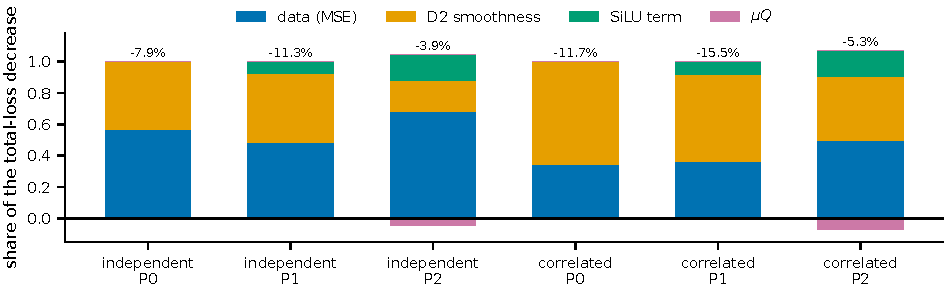
\includegraphics[width=\linewidth]{figS1_lossdecomp.pdf}
  % CAPTION-DRAFT: review (numbers from paper2/figures/figS1_lossdecomp.json)
  \caption{Post hoc loss decomposition (synthetic, early$\to$polished): share of the total-loss decrease from each term, pooled over the 8 seeds of each cell. independent P0: data 0.57, D2 0.43 (median total change -7.9\%); independent P1: data 0.49, D2 0.44 (median total change -11.3\%); independent P2: data 0.68, D2 0.20 (median total change -3.9\%); correlated P0: data 0.35, D2 0.65 (median total change -11.7\%); correlated P1: data 0.37, D2 0.55 (median total change -15.5\%); correlated P2: data 0.50, D2 0.40 (median total change -5.3\%).}
  \label{fig:S1}
\end{figure}


\begin{figure}[h]
  \centering
  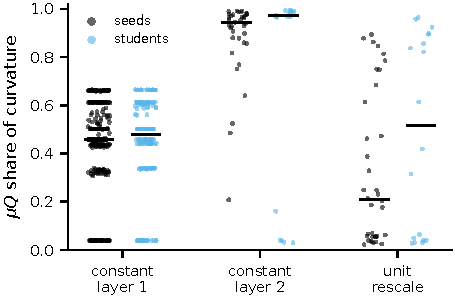
\includegraphics[width=0.5\linewidth]{figS2_gaugecheck.pdf}
  % CAPTION-DRAFT: review (numbers from paper2/figures/figS2_gaugecheck.json)
  \caption{Post hoc gauge check at the $\mu = 10^{-4}$ certified minima: share of the curvature along each least-squares gauge direction contributed by $\mu Q$. Medians: constant shift in layer 1, real-data seeds 0.46 ($n = 288$); constant shift in layer 1, students (trained on a frozen teacher) 0.48 ($n = 144$); constant shift in layer 2, real-data seeds 0.94 ($n = 36$); constant shift in layer 2, students 0.97 ($n = 18$); unit rescaling, real-data seeds 0.21 ($n = 36$); unit rescaling, students 0.52 ($n = 18$).}
  \label{fig:S2}
\end{figure}


\begin{figure}[h]
  \centering
  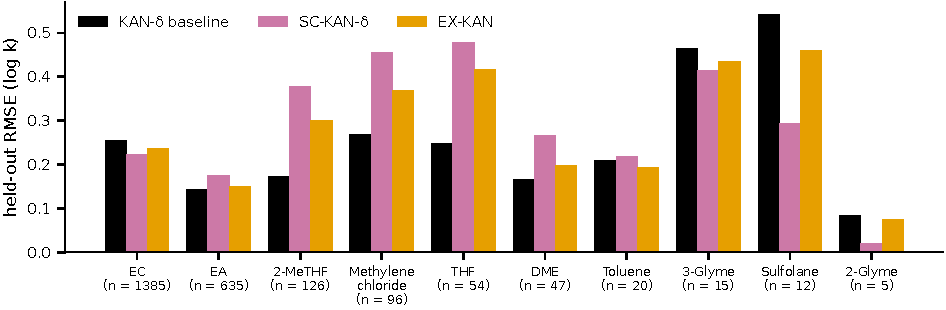
\includegraphics[width=\linewidth]{figS3_loco.pdf}
  % CAPTION-DRAFT: review (numbers from paper2/figures/figS3_loco.json)
  \caption{Leave-one-co-solvent-out RMSE per fold (5-seed ensembles, early state) for the KAN-$\delta$ baseline, SC-KAN-$\delta$ and EX-KAN. Unweighted means: KAN-$\delta$ baseline 0.2554; SC-KAN-$\delta$ 0.2923; EX-KAN 0.2834. The EA fold uses the fold A rows.}
  \label{fig:S3}
\end{figure}

\else % commit hashes replaced by neutral labels (commitmap.json is not part of the submission)
  % GENERATED by build_tex.py (anonymous: commit hashes replaced by labels, see commitmap.json)
\section{All pre-registered predictions}\label{app:prereg}

Generated by \texttt{F-01} from the committed verdict sections; the cell text is the committed wording. Commits are given as pre-registration $\to$ results (in the anonymous version, as neutral labels S-NN). Thresholds are part of each prediction's wording.

\subsection{Synthetic study (\texttt{F-02})}

{\footnotesize\setlength{\tabcolsep}{3pt}
\begin{longtable}{R{0.05\linewidth} R{0.29\linewidth} R{0.36\linewidth} R{0.09\linewidth} R{0.11\linewidth}}
\toprule
ID & Prediction (threshold) & Result & Verdict & Commits \\
\midrule
\endhead
X1 & runaway ($\geq$ 10) in correlated P0 and P1; $\leq$ 3 in the three independent cells and correlated P2 & Correlated P0 $\times$65.7 and P1 $\times$32.1, and P2 $\times$1.00, as predicted. \textbf{But independent P0 $\times$12.5 and P1 $\times$7.9 exceed 3} (independent P2 $\times$1.09) & \textbf{failed} & S-35$\to$\allowbreak S-36 \\
X2 & certified $\leq$ 2/8 in correlated P0 and P1; $\geq$ 6/8 elsewhere & correlated P0 0/8, P1 0/8; independent 6/8, 6/8, 8/8; correlated P2 8/8 & \textbf{held} & S-35$\to$\allowbreak S-36 \\
X3 & cancellation in correlated P0 and P1 each $\geq$ 2 $\times$ correlated P2 & P0 3.29 and P1 2.32, against 2 $\times$ 1.99 = 3.98 & \textbf{failed} & S-35$\to$\allowbreak S-36 \\
X4 & off-manifold ratio $\geq$ 3 in correlated P0 and P1, $\leq$ 1.5 in P2 & P0 1.22, P1 \textbf{0.77}; P2 0.78 (the P2 part held) & \textbf{failed} & S-35$\to$\allowbreak S-36 \\
X5 & Spearman(cancellation, off-manifold RMSE) $\geq$ 0.6 over the 24 correlated models & $\rho$ = +0.177, p = 0.407 & \textbf{failed} & S-35$\to$\allowbreak S-36 \\
X6 & unit match $\geq$ 0.85 in the independent cells and correlated P2; < 0.7 in correlated P0 and P1 & The first part held: 1.000 in all four no-runaway-predicted cells. \textbf{The second part failed: correlated P0 0.774 and P1 0.883 are not < 0.7} & \textbf{failed} & S-35$\to$\allowbreak S-36 \\
\bottomrule
\end{longtable}}
\subsection{Real-data case study (\texttt{F-03})}

Rows are as committed in the case-study summary (one row may cover several predictions, e.g.\ F2--F5). The rank intervention's verdicts are given per arm in the result column.

{\footnotesize\setlength{\tabcolsep}{3pt}
\begin{longtable}{R{0.14\linewidth} R{0.26\linewidth} R{0.29\linewidth} R{0.10\linewidth} R{0.11\linewidth}}
\toprule
Study & Prediction (threshold) & Result & Verdict & Commits \\
\midrule
\endhead
Gauge study (\texttt{gauge\_\allowbreak{}F-04}) & \textbf{Control 1}: teacher edges recovered, median dense corr $\geq$ 0.8 & 0.301 (sanity: h corr 0.913 < 0.95) & \textbf{failed} & S-02$\to$\allowbreak{}S-03 \\
Gauge study (\texttt{gauge\_\allowbreak{}F-04}) & P1: gauge fixing removes $\geq$ 50\% of edge variance & not run & inconclusive (gated by Control 1) & S-02$\to$\allowbreak{}S-03 \\
Gauge study (\texttt{gauge\_\allowbreak{}F-04}) & P2: sparse $\geq$ 2$\times$ dense, DEC region highest & not run & inconclusive (gated) & S-02$\to$\allowbreak{}S-03 \\
Gauge study (\texttt{gauge\_\allowbreak{}F-04}) & P3: (e) < (d) < (c) < (a) & not run & inconclusive (gated) & S-02$\to$\allowbreak{}S-03 \\
Gauge study (\texttt{gauge\_\allowbreak{}F-04}) & P4: every seed has a unit with |corr| < 0.8 & not run & inconclusive (gated) & S-02$\to$\allowbreak{}S-03 \\
Gauge study (\texttt{gauge\_\allowbreak{}F-04}) & P5: KAN-full edge variance > KAN-delta & not run & inconclusive (gated) & S-02$\to$\allowbreak{}S-03 \\
Gauge study (\texttt{gauge\_\allowbreak{}F-04}) & P6: seed spread flags errors & Spearman +0.169 (A) / +0.213 (B); fold B RMSE at 80\% coverage 0.153 vs random 0.137 & \textbf{failed} & S-02$\to$\allowbreak{}S-04 \\
Control 2 (\texttt{control2\_\allowbreak{}F-04}) & C1: (I,C) edges $\geq$ 0.9 and units $\geq$ 0.9 & prediction corr 0.947 < 0.99 & inconclusive (gate failed) & S-05$\to$\allowbreak{}S-06 \\
Control 2 (\texttt{control2\_\allowbreak{}F-04}) & C2: (R,C) invT, molal $\geq$ 0.9; co-solvent < 0.7 & prediction corr 0.969 < 0.99 & inconclusive (gate failed) & S-05$\to$\allowbreak{}S-06 \\
Control 2 (\texttt{control2\_\allowbreak{}F-04}) & C3: 107 epochs gives prediction corr < 0.95 & 0.858 (I,S), 0.919 (R,S) & \textbf{held} & S-05$\to$\allowbreak{}S-06 \\
Control 3 (\texttt{control3\_\allowbreak{}F-04}) & C1': (I) passes the gate, edges $\geq$ 0.9, units $\geq$ 0.9 & (I) RMSE/std 0.128 > 0.05; unit match 0.648 & \textbf{failed} & S-07$\to$\allowbreak{}S-08 \\
Control 3 (\texttt{control3\_\allowbreak{}F-04}) & C2': (R) edges $\leq$ (I) edges $-$ 0.10 & (R) edges 0.852, units 0.659 & inconclusive ((I) failed the gate) & S-07$\to$\allowbreak{}S-08 \\
Control 3 (\texttt{control3\_\allowbreak{}F-04}) & C4: every continuous input $\geq$ 0.9 in (I) & -- & inconclusive ((I) failed the gate) & S-07$\to$\allowbreak{}S-08 \\
Fiber (\texttt{fiber\_\allowbreak{}F-04}) & F1: $\geq$ 50\% of seed pairs on-fiber & 0/190 (closest d = 0.146) & \textbf{failed} & S-09$\to$\allowbreak{}S-10 \\
Fiber (\texttt{fiber\_\allowbreak{}F-04}) & F2--F5 & not run & inconclusive (no on-fiber pairs) & S-09$\to$\allowbreak{}S-10 \\
Fiber 2 (\texttt{fiber2\_\allowbreak{}F-04}) & G1: $\geq$ 4/6 seeds and $\geq$ 10/20 students certify convergence & 0/6, 0/20 (all at the 20,000-iteration cap) & \textbf{failed} & S-11$\to$\allowbreak{}S-12 \\
Fiber 2 (\texttt{fiber2\_\allowbreak{}F-04}) & G2--G5 & not run & inconclusive (no converged model) & S-11$\to$\allowbreak{}S-12 \\
Support (\texttt{support\_\allowbreak{}F-04}) & H1: dim(N) $\geq$ 5 & dim(N) = 36 of 72 & \textbf{held} & S-13$\to$\allowbreak{}S-14 \\
Support (\texttt{support\_\allowbreak{}F-04}) & H2: $\geq$ 50\% of N is REDISTRIBUTION within the correlated group & 18/36 & \textbf{held, exactly at threshold} & S-13$\to$\allowbreak{}S-14 \\
Support (\texttt{support\_\allowbreak{}F-04}) & H3: set A fraction in N $\geq$ 0.5 and $\geq$ 3$\times$ random & median 0.942 (random 0.5) & inconclusive (untestable: 3 $\times$ 0.5 > 1) & S-13$\to$\allowbreak{}S-14 \\
Support (\texttt{support\_\allowbreak{}F-04}) & H4: set B (capped), same criterion & median 0.949 & inconclusive (untestable) & S-13$\to$\allowbreak{}S-14 \\
Support (\texttt{support\_\allowbreak{}F-04}) & H5: flattest Hessian directions overlap N $\geq$ 0.5 & median 0.885; median layer-1 block share only 0.08 & \textbf{held}, with caveat (see \texttt{support\_\allowbreak{}F-04}) & S-13$\to$\allowbreak{}S-14 \\
Support (\texttt{support\_\allowbreak{}F-04}) & H6: fraction in N rises from control-3 to capped state, $\geq$ 15/20 & 20/20 (0.713 $\to$\allowbreak{} 0.949) & \textbf{held} & S-13$\to$\allowbreak{}S-14 \\
Rule (\texttt{rule\_\allowbreak{}F-04}) & I1--I5 (gate) & 0 columns removed; gate stopped & inconclusive & S-16$\to$\allowbreak S-17 \\
Rank (\texttt{rank\_\allowbreak{}F-04}) & I1: median max|grad| $\leq$ 0.1 $\times$ baseline & arm G: \textbf{failed} (4.00$\times$); arm F: \textbf{failed} (29.1$\times$) & see result & S-18$\to$\allowbreak S-19 \\
Rank (\texttt{rank\_\allowbreak{}F-04}) & I2: median d\_AB $\leq$ 0.5 $\times$ baseline & arm G: \textbf{failed} (0.945$\times$); arm F: \textbf{failed} (0.808$\times$) & see result & S-18$\to$\allowbreak S-19 \\
Rank (\texttt{rank\_\allowbreak{}F-04}) & I3 (sanity): median loss $\leq$ 1.10 $\times$ baseline & arm G: passed (1.004$\times$); arm F: passed, narrowly (1.099$\times$) & see result & S-18$\to$\allowbreak S-19 \\
Rank (\texttt{rank\_\allowbreak{}F-04}) & I4: fold A RMSE $\leq$ 0.150 (KAN-delta 0.1420) & arm G: \textbf{held}, narrowly (0.1499); arm F: \textbf{failed} (0.1587) & see result & S-18$\to$\allowbreak S-19 \\
Rank (\texttt{rank\_\allowbreak{}F-04}) & I5: edge corr on 1000/T and molality $\geq$ baseline + 0.1 (baseline 0.102) & arm G: \textbf{held} (0.927); arm F: \textbf{held} (0.338) & see result & S-18$\to$\allowbreak S-19 \\
Rank (\texttt{rank\_\allowbreak{}F-04}) & I6: arm F's improvement $\geq$ arm G's in both I1 and I2 & arm G: \textbf{failed} (max|grad| 29.1$\times$ vs 4.00$\times$; d\_AB does favour F, 0.808 vs 0.945) & see result & S-18$\to$\allowbreak S-19 \\
\texttt{trust\_\allowbreak{}F-04} & T1 / T2: trust-krylov certifies $\geq$ 4/6 seeds / $\geq$ 2/3 students & 0/6, 0/3. All 9 stopped on scipy's "bad approximation" after 1--62 iterations; the Hessian was accurate to $\leq$ 2e-7 & \textbf{failed} & S-20$\to$\allowbreak S-21 \\
\texttt{trust\_\allowbreak{}F-04} & T3--T5 & nothing converged & inconclusive & S-20$\to$\allowbreak S-21 \\
\texttt{stage2\_\allowbreak{}F-04} & U1: trust-exact (exact Hessian, 500 iterations) certifies $\geq$ 4/6 seeds & 0/6. All 9 hit the iteration cap & \textbf{failed} & S-22$\to$\allowbreak S-26 \\
\texttt{stage2\_\allowbreak{}F-04} & U2: with L2 $\lambda$ = 1e-5, $\geq$ 4/6 seeds and $\geq$ 2/3 students & 1/6 seeds, 0/3 students & \textbf{failed} & S-22$\to$\allowbreak S-26 \\
\texttt{stage2\_\allowbreak{}F-04} & U3: more converge at 1e-5 than at 1e-6 & 1 vs 0 & \textbf{held} & S-22$\to$\allowbreak S-26 \\
\texttt{stage2\_\allowbreak{}F-04} & U4: converged L2 models' loss without L2 $\leq$ 1.05 $\times$ capped & 1.2545 & \textbf{failed} & S-22$\to$\allowbreak S-26 \\
\texttt{stage2\_\allowbreak{}F-04} & U5: converged seeds' disagreement $\leq$ 0.5 $\times$ capped & only 1 converged & inconclusive & S-22$\to$\allowbreak S-26 \\
\texttt{close\_\allowbreak{}F-04} & V1: at some $\mu$, $\geq$ 4/6 seeds and $\geq$ 2/3 students converge (stage2 criterion) & 0 certified at every $\mu$ & \textbf{failed} & S-29$\to$\allowbreak{}S-30 \\
\texttt{close\_\allowbreak{}F-04} & V2: converged seeds' data term $\leq$ 1.05 $\times$ stage2 A & nothing certified at the selected $\mu$ = 1e-6 & inconclusive & S-29$\to$\allowbreak{}S-30 \\
\texttt{close\_\allowbreak{}F-04} & V3: $\|\theta\|^{2}$ $\leq$ 10 $\times$ start & same & inconclusive & S-29$\to$\allowbreak{}S-30 \\
\texttt{close\_\allowbreak{}F-04} & V4: seed disagreement halved & same & inconclusive & S-29$\to$\allowbreak{}S-30 \\
\texttt{close\_\allowbreak{}F-04} & V5: students' unit match $\geq$ 0.8 & same & inconclusive & S-29$\to$\allowbreak{}S-30 \\
\texttt{close\_\allowbreak{}F-04} & V6: fold A RMSE $\leq$ 0.150 & 1.0262, bias +0.9028 & \textbf{failed} & S-29$\to$\allowbreak{}S-30 \\
\texttt{certify\_\allowbreak{}F-04} & W1: at $\mu$ = 1e-4, $\geq$ 5/6 seeds certified (second-order criterion, F-a) & 6/6; all 17 candidates certified & \textbf{held} & S-31$\to$\allowbreak{}S-32 \\
\texttt{certify\_\allowbreak{}F-04} & W2: certified seeds' median d\_AB $\leq$ 0.5 $\times$ capped & 0.0771 vs capped 0.1041 ($-$26\%) & \textbf{failed} & S-31$\to$\allowbreak{}S-32 \\
\texttt{certify\_\allowbreak{}F-04} & W3: certified students' unit match $\geq$ 0.8 (vs the original teacher) & 0.624 & \textbf{failed} & S-31$\to$\allowbreak{}S-32 \\
\texttt{certify\_\allowbreak{}F-04} & W4: $\mu$ = 1e-4 fold A RMSE $\leq$ 0.150 & 0.3345 & \textbf{failed} & S-31$\to$\allowbreak{}S-32 \\
\texttt{certify\_\allowbreak{}F-04} & W5: $\mu$ = 1e-4 fold A RMSE $\leq$ 0.5131 & 0.3345 & \textbf{held} & S-31$\to$\allowbreak{}S-32 \\
\texttt{certify\_\allowbreak{}F-04} & W6: Spearman(cross-edge ratio, held-out RMSE) $\geq$ 0.6 & $\rho$ = +0.345, p = 0.328 (weak test) & \textbf{failed} & S-31$\to$\allowbreak{}S-32 \\
\bottomrule
\end{longtable}}
\noindent Committed tally of the case study:

{\footnotesize\setlength{\tabcolsep}{3pt}
\begin{longtable}{R{0.55\linewidth} r r r}
\toprule
Study & Held & Failed & Inconclusive \\
\midrule
\endhead
First table (Control 1, P1--P6, C1--C3, C1'/C2'/C4, F1--F5, G1--G5, H1--H6) & 5 & 5 & 19 \\
Rule (I1--I5) & 0 & 0 & 5 \\
Rank (I1, I2, I4, I5 per arm, I6) & 3 & 6 & 0 \\
Trust (T1--T5) & 0 & 2 & 3 \\
Stage 2 (U1--U5) & 1 & 3 & 1 \\
Close (V1--V6) & 0 & 2 & 4 \\
Certify (W1--W6) & 2 & 4 & 0 \\
\textbf{Total} & \textbf{11} & \textbf{22} & \textbf{32} \\
\bottomrule
\end{longtable}}
\subsection{Shared-curve KAN (\texttt{F-05})}

Run after the case-study close-out; not part of the 65 predictions above.

{\footnotesize\setlength{\tabcolsep}{3pt}
\begin{longtable}{R{0.05\linewidth} R{0.26\linewidth} R{0.39\linewidth} R{0.09\linewidth} R{0.11\linewidth}}
\toprule
ID & Prediction (threshold) & Result & Verdict & Commits \\
\midrule
\endhead
S1 & SC LOCO RMSE $\leq$ 1.05 $\times$ baseline & unweighted mean SC 0.2923 vs base 0.2554 (ratio 1.145; threshold 0.2681). Also reported: row-weighted 0.2478 / 0.2297 (1.079); folds $\geq$ 20 rows 0.3138 / 0.2093 (1.499) & failed & S-38$\to$\allowbreak S-40 \\
S2 & SC fold A RMSE $\leq$ 0.160 & SC 0.1757 (base 0.1420) & failed & S-38$\to$\allowbreak S-40 \\
S3 & SC median d\_AB $\leq$ 0.5 $\times$ baseline & SC 0.1865 vs base 0.1120 (threshold 0.0560): SC seeds agree \emph{less} than baseline seeds & failed & S-38$\to$\allowbreak S-40 \\
S4 & curve corr $\geq$ 0.90 for $\geq$ 6 of 8 inputs & 3 of 8 (M\_co 0.959, mix\_lneta 0.970, invT 0.986); lowest x\_co 0.596; others 0.871--0.891 & failed & S-38$\to$\allowbreak S-40 \\
S5 & $\geq$ 8/10 SC fold A models certified & SC 10/10 (max|grad| $\leq$ 7e-10, 0 near-null eigenvalues); baseline 0/10 (all hit the 500-iteration cap) & held & S-38$\to$\allowbreak S-40 \\
S6 & median $\beta$-norm polished/early $\leq$ 3 (calibrated) & median 1.337 (range 0.652--2.356); $\|\theta\|^{2}$ $\times$4.59 (base $\times$67.9, range 30.6--281) & held & S-38$\to$\allowbreak S-40 \\
S7 & SC polished/early fold A RMSE $\leq$ 1.5 & SC 1.920 (0.1757 $\to$\allowbreak{} 0.3373); baseline 5.736 (0.1420 $\to$\allowbreak{} 0.8147) & failed & S-38$\to$\allowbreak S-40 \\
S8 & d log k/d(1000/T) < 0 on $\geq$ 95\% rows in $\geq$ 8/10 seeds & 10/10 (median share 1.000; 1424 rows, 10 excluded per D4) & held & S-38$\to$\allowbreak S-40 \\
S9 & Spearman(1000/T, |slope|) > 0 in $\geq$ 8/10 seeds & 10/10 (median +0.661, range +0.406 to +0.885) & held & S-38$\to$\allowbreak S-40 \\
S10 & d log k/d(ln $\eta$\_mix) < 0 on $\geq$ 90\% rows in $\geq$ 8/10 seeds & 7/10 (median share 0.967; s0 0.892, s2 0.892, s8 0.826) & failed & S-38$\to$\allowbreak S-40 \\
\bottomrule
\end{longtable}}
\subsection{Two-anchor excess model (\texttt{F-06})}

Run after the case-study close-out; not part of the 65 predictions above.

{\footnotesize\setlength{\tabcolsep}{3pt}
\begin{longtable}{R{0.05\linewidth} R{0.26\linewidth} R{0.39\linewidth} R{0.09\linewidth} R{0.11\linewidth}}
\toprule
ID & Prediction (threshold) & Result & Verdict & Commits \\
\midrule
\endhead
E1 & EX LOCO $\leq$ 0.95 $\times$ KAN-delta & unweighted mean EX 0.2834 vs threshold 0.2426 (base 0.2554; ratio 1.110). Row-weighted 0.2363 / 0.2297 (1.029); folds $\geq$ 20 rows 0.2662 / 0.2093 (1.272). EX is better on EC (0.237 vs 0.256), Sulfolane, 3-Glyme, 2-Glyme and Toluene, and worse on 2-MeTHF, THF, Methylene chloride, DME and EA & failed & S-41$\to$\allowbreak S-43 \\
E2 & EX fold A $\leq$ 0.142 & EX 0.1502 (base this run 0.1420) & failed & S-41$\to$\allowbreak S-43 \\
E3 & s agrees across seeds (separable co-solvents, Amendment 1) & median pairwise corr +0.987 over EA, EC, Methylene chloride: a weak test with 3 values per seed, and Methylene chloride is marginal. Seed SD of s: EA 0.063 (0.39 $\times$ the spread across co-solvents, 0.159), EC 0.091 (0.57 $\times$), Methylene chloride 0.067 (0.42 $\times$). Secondary ($\leq$ 2 rule, 7 co-solvents): +0.869 & held & S-41$\to$\allowbreak S-43 \\
E4 & mean s(low $\varepsilon$) < mean s(EC, Sulfolane) in $\geq$ 8/10 seeds & 0/10: the ordering is reversed in every seed. Per high-$\varepsilon$ co-solvent: vs EC alone 0/10 (EC median s +0.104), vs Sulfolane alone 0/10 (median $-$0.124). The low-$\varepsilon$ mean is +0.19 to +0.49 per seed. Sulfolane does not drive the failure on its own: EC alone fails in every seed too & failed & S-41$\to$\allowbreak S-43 \\
E5 & median seed-SD flagged $\geq$ 2 $\times$ separable (Amendment 1) & 0.091 vs 0.067, ratio 1.37. Secondary ($\leq$ 2 rule): 0.222 vs 0.069, ratio 3.22, no verdict; the secondary is driven by 3-Glyme (SD 0.478, M\_co extrapolated) and 2-Glyme (0.222) & failed & S-41$\to$\allowbreak S-43 \\
\bottomrule
\end{longtable}}% GENERATED by build_tex.py (anonymous: commit hashes replaced by labels, see commitmap.json)
\section{Post-hoc analyses}\label{app:posthoc}

Every analysis below was defined after seeing results. Each is labelled \textbf{post hoc} in its own files, changes no pre-registered verdict, and is reported as exploratory. The description is the subject line of the commit that added the analysis.

{\footnotesize\setlength{\tabcolsep}{3pt}\begin{longtable}{R{0.28\linewidth} R{0.52\linewidth} R{0.10\linewidth}}
\toprule
Analysis & Commit subject (as committed) & Commit \\
\midrule
\endhead
\textbf{Post hoc.} Anatomy of the real-data runaway \newline \footnotesize{\texttt{F-07, F-08, F-09}} & Plan for descriptive runaway anatomy (before F-08 exists) & S-27 \\
 & Anatomy (descriptive): Q1, Q2 not as expected, Q3 as expected; RBF growth is in the penalty null space & S-28 \\
\textbf{Post hoc.} Gauge check and regularised teacher (exploratory) \newline \footnotesize{\texttt{F-10, F-11, F-12}} & gaugecheck (POST-HOC, exploratory): penalty fixes gauge position by slope balance; students match the regularised teacher & S-33 \\
\textbf{Post hoc.} Anatomy of the synthetic runaway \newline \footnotesize{\texttt{F-13, F-14}} & paper2 anatomy\_synth (POST-HOC, descriptive): synthetic runaway lives mainly in layer-2 output-edge cancellation, unsaturated; no verdicts change & S-37 \\
\textbf{Post hoc.} Loss decomposition along the runaway \newline \footnotesize{\texttt{F-15, F-16}} & paper2 lossdecomp (POST-HOC, descriptive): synthetic runaway loss decrease shared, D2 penalty median 0.61 vs data 0.37; 12/20 runaway models overfit; real-data reference recomputed & S-44 \\
\textbf{Post hoc.} Descriptive checks (hidden-unit correlation, tilt affinity, references) \newline \footnotesize{\texttt{F-17, F-18, F-19}} & paper2/checks: plan for descriptive checks (F4 hidden-unit correlation, F2 tilt affinity, A1 commit and data citation) before F-20 exists & S-46 \\
 & paper2/checks (POST-HOC, descriptive): hidden-unit correlation marks the runaway (independent cells 0.70 vs 0.05) but is not sufficient; RBF tilt affine to 2\% centrally, 13\% at the ends; A1 commit S-01; CALiSol-23 citation not in competition material & S-47 \\
\textbf{Post hoc.} Regularised teacher (weights pinned) & Pin gaugecheck regularised-teacher weights in a seventh archive; append to weights manifest & S-34 \\
\bottomrule
\end{longtable}}% GENERATED by build_tex.py (anonymous: commit hashes replaced by labels, see commitmap.json)
\section{Reproducibility map}\label{app:repro}

Generated from \texttt{F-42}. Every figure is rebuilt by its script from committed results; each figure's sidecar JSON lists the data files (path, commit, SHA-256), any archived weights (SHA-256, archive) and every plotted number. \REPOSTATEMENT

{\footnotesize\setlength{\tabcolsep}{3pt}
\begin{longtable}{R{0.15\linewidth} R{0.13\linewidth} R{0.42\linewidth} R{0.19\linewidth}}
\toprule
Figure & Script & Data files (commit) & Archived weights \\
\midrule
\endhead
Figure~\ref{fig:mechanism} \figname{fig1\_mechanism} & \texttt{F-43} & none (computed from committed code: F-02, F-44) & --- \\
Figure~\ref{fig:synthetic} \figname{fig2\_synthetic} & \texttt{F-45} & \texttt{F-46} (S-36) & --- \\
Figure~\ref{fig:where} \figname{fig3\_where} & \texttt{F-47} & \texttt{F-48} (S-88); \texttt{F-49} (S-37); \texttt{F-50} (S-48) & 18 files, archives W-01, W-02, W-03 \\
Figure~\ref{fig:applicability} \figname{fig4\_applicability} & \texttt{F-51} & \texttt{F-34} (S-90); \texttt{F-48} (S-88) & 15 files, archives W-04, W-05, W-06 \\
Figure~\ref{fig:paths} \figname{fig5\_paths} & \texttt{F-52} & \texttt{F-53} (S-59) & --- \\
Figure~\ref{fig:corrdose} \figname{fig6\_correlation\_dose} & \texttt{F-54} & \texttt{F-55} (S-64) & --- \\
Figure~\ref{fig:bspline} \figname{fig7\_bspline} & \texttt{F-56} & \texttt{F-46} (S-36); \texttt{F-57} (S-81); \texttt{F-30} (S-86) & --- \\
Figure~\ref{fig:dose} \figname{fig8\_dose\_response} & \texttt{F-58} & \texttt{F-59} (S-26); \texttt{F-60} (S-30); \texttt{F-61} (S-32) & --- \\
Figure~\ref{fig:uniqueness} \figname{fig9\_uniqueness} & \texttt{F-62} & \texttt{F-63} (S-41); \texttt{F-61} (S-32); \texttt{F-48} (S-88) & 40 files, archives W-05 \\
Figure~\ref{fig:S1} \figname{figS1\_lossdecomp} & \texttt{F-64} & \texttt{F-65} (S-46) & --- \\
Figure~\ref{fig:S2} \figname{figS2\_gaugecheck} & \texttt{F-64} & \texttt{F-66} (S-33) & --- \\
Figure~\ref{fig:S3} \figname{figS3\_loco} & \texttt{F-64} & \texttt{F-63} (S-41); \texttt{F-67} (S-45) & --- \\
\bottomrule
\end{longtable}}
\noindent Tables in the main text (no script; values typed in the draft):

{\footnotesize\setlength{\tabcolsep}{3pt}
\begin{longtable}{R{0.14\linewidth} R{0.14\linewidth} R{0.45\linewidth} R{0.16\linewidth}}
\toprule
Table & Source & Data files & Commits \\
\midrule
\endhead
Table~\ref{tab:synthetic} & typed in the draft from & \texttt{F-46}, \texttt{F-68} & S-36 \\
Table~\ref{tab:dose} & typed in the draft from & \texttt{F-60}, \texttt{F-61}, \texttt{F-59} & S-30, S-32, S-26 \\
Table~\ref{tab:alternatives} & typed in the draft from & \texttt{F-63}, \texttt{F-67}, \texttt{F-69} & S-41, S-45, S-49 \\
\bottomrule
\end{longtable}}
\noindent Panels evaluated post hoc from archived weights (from \texttt{F-70}):

\begin{itemize}
  \item \textbf{fig3a, real data:} the split of the parameter change into affine and curved RBF parts per layer, for 107 epochs $\to$\allowbreak{} fiber2 capped $\to$\allowbreak{} stage2 Part A.
  \item \texttt{F-59} stores only per-block norms, without an affine/curved split and without the 107 $\to$\allowbreak{} capped change.
  \item \textbf{fig9b, polished fold A d\_AB} for SC-KAN-$\delta$ and the baseline (marked *).
  \item arch/sc committed d\_AB only at the early state.
  \item \textbf{fig4a, b, fold A per-row error change} (early-stopped -> mu = $10^{-6}$ and mu = $10^{-4}$ ensembles).
  \item F-71 stores only the per-row Spearman correlations and medians; the per-row values are re-evaluated with the
\end{itemize}% GENERATED by build_tex.py (anonymous: commit hashes replaced by labels, see commitmap.json)
\section{Research process}\label{app:process}

% DRAFT-TEXT: review (new prose, not in the source draft; it states only the protocol followed, no results). First and last paragraphs: author-supplied wording (2026-10-05)
\paragraph{Pre-registration.} Every study committed a pre-registration file (predictions, thresholds, interpretation rules) before the script that tested it existed. Verdicts were appended below the committed text; the pre-registered text was never edited, and corrections to reported numbers were made in separate, labelled commits.
\paragraph{Amendments.} A change to a design after its pre-registration was committed as a dated amendment section before any affected model was trained, with its reason; the original text was kept. Choices forced by the code or data at run time were logged as numbered discrepancies at the top of each output log.
\paragraph{Files win.} Instructions to the agent stated that committed files take precedence over any number or description in a prompt; discrepancies between a brief and the files were flagged rather than resolved silently.
\paragraph{Data and weights.} Model weights were never committed: they were archived outside the repository with a manifest of SHA-256 hashes and producing commits, and every later analysis verified the hashes and held its inputs in memory. Post-hoc analyses were labelled as such in their files and changed no verdict.
\paragraph{AI assistance.} Code, runs and logs were produced by an AI coding agent working under this protocol. Study designs, briefs and the manuscript were developed with an AI assistant. The author set the research questions, reviewed and approved every brief and amendment, decided each next stage, and takes responsibility for all content. Crashes were recorded in the logs and fixed in separate commits labelled as implementation-only.

\noindent Pre-registrations, amendments and crash records (from the commit history):

{\footnotesize\setlength{\tabcolsep}{3pt}
\begin{longtable}{R{0.08\linewidth} R{0.10\linewidth} R{0.14\linewidth} R{0.58\linewidth}}
\toprule
Commit & Date & Kind & Commit subject \\
\midrule
\endhead
S-02 & 2026-09-23 & pre-registration & Pre-register KAN identifiability study (before any experiment) \\
S-05 & 2026-09-23 & pre-registration & Pre-register corrected 2x2 control (before writing or running it) \\
S-07 & 2026-09-23 & pre-registration & Pre-register control 3: reachable teacher (before writing code) \\
S-09 & 2026-09-29 & pre-registration & Pre-register fiber completeness test (before writing or running F-41) \\
S-11 & 2026-09-29 & pre-registration & Pre-register fiber2: certified convergence + teacher-known fiber analysis (before writing code) \\
S-13 & 2026-09-29 & pre-registration & Pre-register support study: near-null space, where models differ, Hessian (before F-42 exists) \\
S-15 & 2026-09-29 & pre-registration & Close-out: electrolyte case study summary (all pre-registered predictions) \\
S-16 & 2026-09-29 & pre-registration & Pre-register basis-size rule intervention (before F-43 exists) \\
S-18 & 2026-09-29 & pre-registration & Pre-register rank-constrained layer-1 intervention (before F-44 exists) \\
S-20 & 2026-09-30 & pre-registration & Pre-register trust-region Newton polishing, stage 1 (before F-45 exists) \\
S-22 & 2026-09-30 & pre-registration & Pre-register stage 2: trust-exact check, runaway diagnostic, coercivity (before F-46 exists) \\
S-23 & 2026-09-30 & crash record / fix & F-46 as first run (crashed with AttributeError in callback) \\
S-24 & 2026-09-30 & crash record / fix & stage2: fix AttributeError (implementation only, post-prereg) \\
S-25 & 2026-10-02 & crash record / fix & stage2: hold verified inputs in memory (implementation only, post-prereg) \\
S-29 & 2026-10-02 & pre-registration & Pre-register targeted null-space penalty intervention (before F-47 exists) \\
S-31 & 2026-10-03 & pre-registration & Pre-register second-order certification and regularised fold A accuracy (before F-48 exists) \\
S-35 & 2026-10-03 & pre-registration & paper2: pre-register synthetic 2x3 runaway test (before F-49 exists) \\
S-38 & 2026-10-03 & pre-registration & arch: pre-register SC-KAN-$\delta$ (shared-curve KAN-$\delta$) before any script exists; decisions C (centring), mu null-space term, tanh salt embedding, full beta term \\
S-39 & 2026-10-03 & crash record / fix & arch sc\_run: fix log() call (crash record 1, after the first fold A polish); resume from cache \\
S-41 & 2026-10-04 & pre-registration & arch: pre-register EX-KAN (two-anchor excess model) before any script exists; decision B (x\_co-independent g, [7,6,1]), full set for E3-E5, E4 mean rule \\
S-42 & 2026-10-04 & amendment & arch ex\_prereg: Amendment 1 (after Step 0, before training): primary separability rule by fixed-composition groups (EA, EC, Methylene chloride separable); committed rule reported as secondary \\
\bottomrule
\end{longtable}}% GENERATED by build_tex.py (anonymous: commit hashes replaced by labels, see commitmap.json)
\section{Supplementary figures}\label{app:supp}


\begin{figure}[htbp]
  \centering
  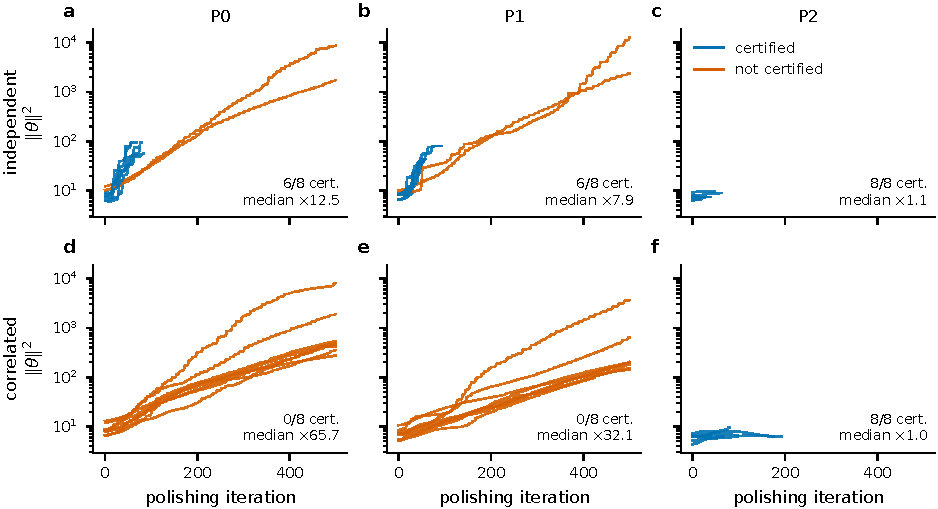
\includegraphics[width=\linewidth]{fig2_synthetic.pdf}
  % CAPTION-DRAFT: review (numbers from paper2/figures/fig2_synthetic.json)
  \caption{Synthetic $2\times3$ study: $\|\theta\|^2$ over exact-Hessian trust-region polishing iterations (log scale), one line per seed, coloured certified (blue) or not certified (vermillion). Rows: independent and correlated inputs; columns: P0, P1, P2. Per panel, certified seeds and median growth (polished over early-stopped): independent P0: 6/8 certified, $\times$12.5; independent P1: 6/8 certified, $\times$7.9; independent P2: 8/8 certified, $\times$1.1; correlated P0: 0/8 certified, $\times$65.7; correlated P1: 0/8 certified, $\times$32.1; correlated P2: 8/8 certified, $\times$1.0.}
  \label{fig:synthetic}
\end{figure}


\begin{figure}[htbp]
  \centering
  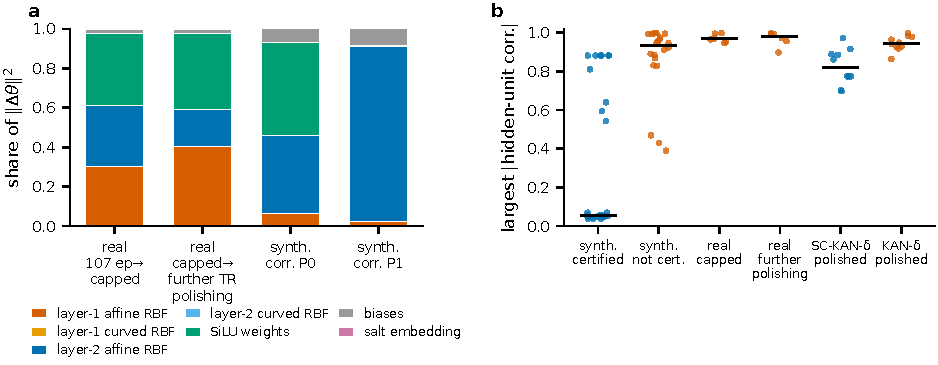
\includegraphics[width=\linewidth]{fig3_where.pdf}
  % CAPTION-DRAFT: review (numbers from paper2/figures/fig3_where.json)
  \caption{Where the runaway lives. \textbf{(a)} Mean share of $\|\Delta\theta\|^2$ by parameter block. Real data, 107 epochs$\to$capped: layer-1 affine RBF 0.30, layer-2 affine RBF 0.31, SiLU weights 0.37; capped$\to$further trust-region polishing: 0.40, 0.19, 0.38; synthetic correlated P0: layer-2 affine RBF 0.39, SiLU weights 0.47; correlated P1: layer-2 affine RBF 0.89. The real-data split was evaluated post hoc from archived weights (Appendix~\ref{app:repro}). \textbf{(b)} Largest absolute correlation between hidden-unit activations on the training rows, median: synthetic, certified 0.054 ($n=28$); synthetic, not certified 0.935 ($n=20$); real, capped 0.968 ($n=6$); real, further polishing 0.983 ($n=6$); SC-KAN-$\delta$ polished 0.818 ($n=10$); KAN-$\delta$ polished 0.946 ($n=10$). Blue: certified; vermillion: not certified or runaway.}
  \label{fig:where}
\end{figure}


\begin{figure}[htbp]
  \centering
  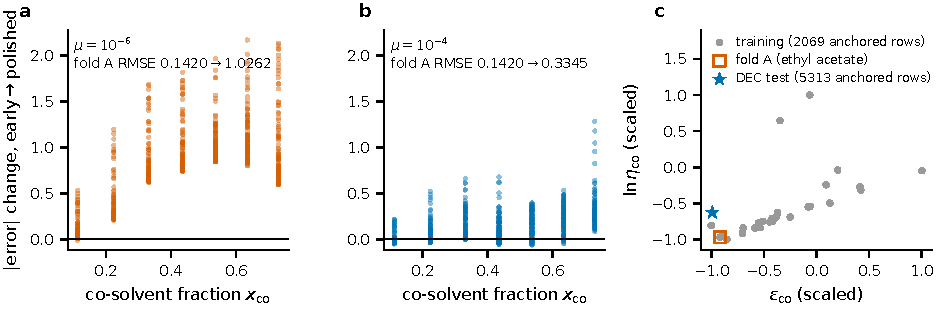
\includegraphics[width=\linewidth]{fig4_applicability.pdf}
  % CAPTION-DRAFT: review (numbers from paper2/figures/fig4_applicability.json)
  \caption{Applicability (descriptive; analysis plan committed before computing). \textbf{(a, b)} Fold A (ethyl acetate held out, 635 rows): change in each row's absolute error from the early-stopped 5-seed ensemble to the polished ensemble, against the co-solvent fraction $x_{\mathrm{co}}$ (7 distinct values); fold A RMSE 0.1420$\to$1.0262 at $\mu = 10^{-6}$ (a) and 0.1420$\to$0.3345 at $\mu = 10^{-4}$ (b). Per-row values are evaluated post hoc from SHA-verified archived weights, with the logged RMSEs reproduced (Appendix~\ref{app:repro}). \textbf{(c)} Co-solvent descriptors $\varepsilon_{\mathrm{co}}$ and $\ln\eta_{\mathrm{co}}$ in the committed min--max scaling: the 2069 anchored training rows (30 distinct points), fold A's co-solvent (off-pattern distance 0.047) and the 5313 anchored DEC test rows (0.334); each held-out set occupies a single point.}
  \label{fig:applicability}
\end{figure}


\begin{figure}[htbp]
  \centering
  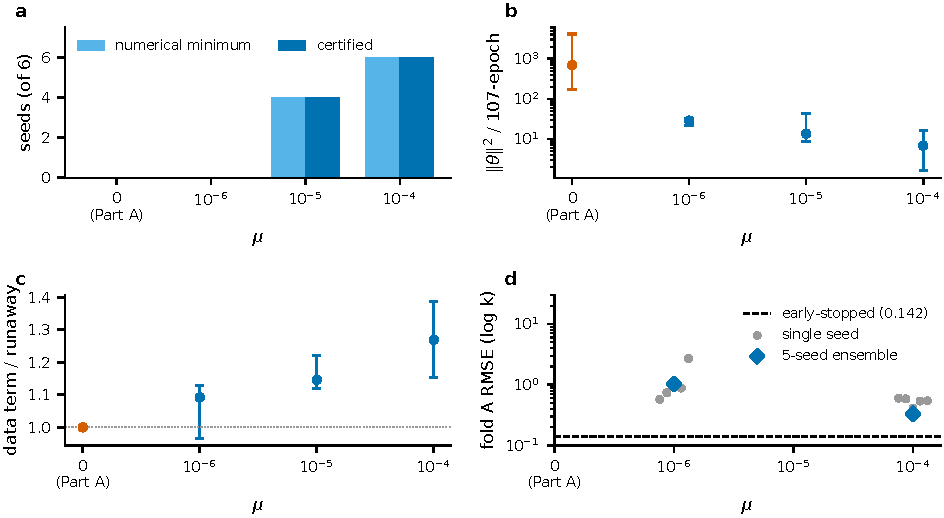
\includegraphics[width=\linewidth]{fig8_dose_response.pdf}
  % CAPTION-DRAFT: review (numbers from paper2/figures/fig8_dose_response.json)
  \caption{Real-data dose-response in the null-space weight $\mu$ (6 KAN-$\delta$ seeds; $\mu = 0$: polished without a null-space penalty). \textbf{(a)} Seeds at a numerical minimum (all of them certified): $\mu = 0$, 0 of 6; $10^{-6}$, 0 of 6; $10^{-5}$, 4 of 6; $10^{-4}$, 6 of 6. \textbf{(b)} $\|\theta\|^2$ relative to the 107-epoch state, median (range): $\mu = 0$, 690 (170--4146); $10^{-6}$, 29 (21--31); $10^{-5}$, 14 (9--43); $10^{-4}$, 7 (2--16). \textbf{(c)} Training data term relative to the runaway, median: $10^{-6}$, 1.092; $10^{-5}$, 1.146; $10^{-4}$, 1.269. \textbf{(d)} Fold A RMSE: early-stopped 0.142 (dashed line); polished 5-seed ensemble 1.026 at $\mu = 10^{-6}$ and 0.334 at $\mu = 10^{-4}$; grey points are single seeds.}
  \label{fig:dose}
\end{figure}


\begin{figure}[h]
  \centering
  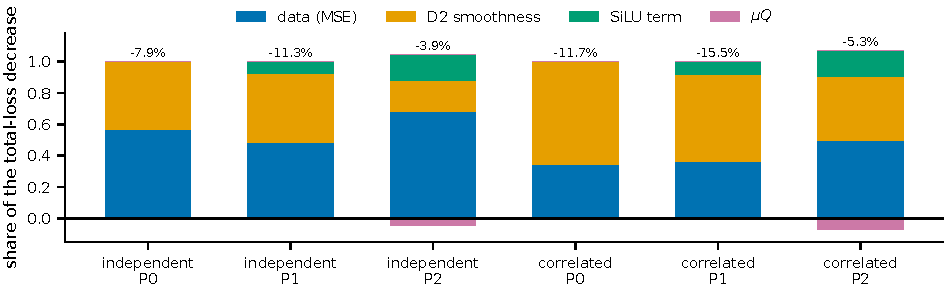
\includegraphics[width=\linewidth]{figS1_lossdecomp.pdf}
  % CAPTION-DRAFT: review (numbers from paper2/figures/figS1_lossdecomp.json)
  \caption{Post hoc loss decomposition (synthetic, early$\to$polished): share of the total-loss decrease from each term, pooled over the 8 seeds of each cell. independent P0: data 0.57, D2 0.43 (median total change -7.9\%); independent P1: data 0.49, D2 0.44 (median total change -11.3\%); independent P2: data 0.68, D2 0.20 (median total change -3.9\%); correlated P0: data 0.35, D2 0.65 (median total change -11.7\%); correlated P1: data 0.37, D2 0.55 (median total change -15.5\%); correlated P2: data 0.50, D2 0.40 (median total change -5.3\%).}
  \label{fig:S1}
\end{figure}


\begin{figure}[h]
  \centering
  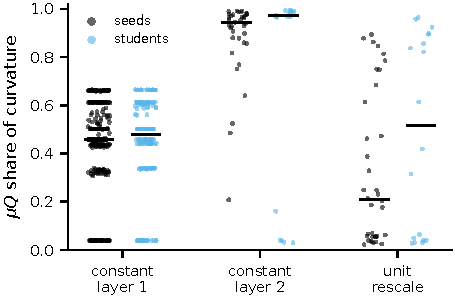
\includegraphics[width=0.5\linewidth]{figS2_gaugecheck.pdf}
  % CAPTION-DRAFT: review (numbers from paper2/figures/figS2_gaugecheck.json)
  \caption{Post hoc gauge check at the $\mu = 10^{-4}$ certified minima: share of the curvature along each least-squares gauge direction contributed by $\mu Q$. Medians: constant shift in layer 1, real-data seeds 0.46 ($n = 288$); constant shift in layer 1, students (trained on a frozen teacher) 0.48 ($n = 144$); constant shift in layer 2, real-data seeds 0.94 ($n = 36$); constant shift in layer 2, students 0.97 ($n = 18$); unit rescaling, real-data seeds 0.21 ($n = 36$); unit rescaling, students 0.52 ($n = 18$).}
  \label{fig:S2}
\end{figure}


\begin{figure}[h]
  \centering
  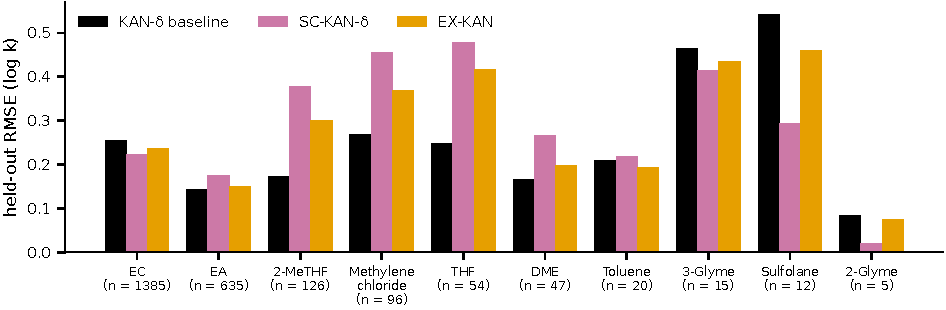
\includegraphics[width=\linewidth]{figS3_loco.pdf}
  % CAPTION-DRAFT: review (numbers from paper2/figures/figS3_loco.json)
  \caption{Leave-one-co-solvent-out RMSE per fold (5-seed ensembles, early state) for the KAN-$\delta$ baseline, SC-KAN-$\delta$ and EX-KAN. Unweighted means: KAN-$\delta$ baseline 0.2554; SC-KAN-$\delta$ 0.2923; EX-KAN 0.2834. The EA fold uses the fold A rows.}
  \label{fig:S3}
\end{figure}

\clearpage  % flush Appendix E's figures before Appendix F
\fi

\end{document}
